\chapter{Evaluation}\label{ch:Evaluation}

In order to evaluate the effectiveness of the newly developed interpolating intersection logic,
three test cases will be used and compared to the snapshot method.
\newline
The first test case is simple: A receiver moves towards an emitter at 1/9th the speed of sound.
It starts 342.2 meters away from the emitter.
The emitter sends out a sine wave at 440Hz for 1 second.
No other objects are in the scene.
\newline
This is essentially the example described in \ref{im:SnapshotExplain}
and is used to demonstrate the basic differences between interpolated and snapshot methods.
\newline
\begin{figure}[t!]
    \includesvg[width=\linewidth]{images/test_rooms.svg}
    \caption{The second (left) and third (right) test scene, with the emitter, receiver and rotation axis all denoted by the black dot.}\label{fig:TestScenes}
\end{figure}
The second test case takes place inside a rotating rectangular room as seen on the left side of \autoref{fig:TestScenes}.
Said room is 4 meters in width and length and 3 meters tall.
The receiver is exactly in the middle of the room,
with the emitter being 1.2 meters above it.
The room rotates around the Z-axis, completing a full rotation once per second.
\newline
This is used to test whether the differences between interpolated and snapshot methods
lead to a notable difference in a slightly more practical scenario.
\newline
The third test case takes place inside a rotating, 2 meters tall L-shaped room,
as denoted on the right side of \autoref{fig:TestScenes},
with the receiver being at the origin at 1 meter height and the emitter being 0.5 meters above it.
The room again rotates around the Z-axis, but takes three seconds for a full rotation.
\newline
This case is used to demonstrate the shortcomings of the interpolating intersection logic
and the need for further research for realistic simulations.

\section{Testing Conditions}

Tests were performed on a stock AMD Ryzen 3600xt CPU with 16GB of 3200MHz DDR4 RAM.
All 12 logical cores are used for parallel processing
and no other programs other than a shell for the program to run in (and Windows 10 background processes) were running to avoid needless interference.
\newline
The proof-of-concept used for testing was written in Rust, using the \verb|nalgebra| crate for algebra functions,
\verb|roots| for polynomial solving and \verb|rayon| for parallelisation.
For simplicity's sake, only an energetic response was calculated, not an impulse response.
This leads to less accurate auralization as phase is disregarded,
but is sufficient to show basic differences between the snapshot and interpolated method.
\newline
The first test case with the approaching receiver is run using one ray per sample
as it only attempts to simulate sound travelling from emitter to receiver
without considering bounces from a room around it.
The ray is always directed at the receiver.
\newline
The other two test cases are run using 10 million rays per sample,
which is enough to get an approximate \(T_{60}\) sufficient to draw conclusions about the scenes
while requiring a reasonable amount of compute time.
To account for variance introduced by randomness, 3 runs are done per simulation method and scene.
\newline
For the two rotating scenes, only one energetic response is calculated and applied to all samples.
This is because the starting condition of a rotating room is always the same:
As both rooms rotate around the emitter's and the receiver's position
and the emitter emits rays randomly in all directions,
the relative position of the room to the receiver and emitter is always the same,
making for the same energetic response at all times.
\newline
Simulations would become much more expensive for scenes where this condition doesn't apply,
as that would mean calculating individual impulse responses for each sample.
For a 1 second sample at 44100 KHz and a roughly 20 minute IR calculation time
(rounded down from the snapshot method test results below),
this would take \(44100 \cdot 20 m = 882000 m = 14700 h = 612.5 d\).
Running simulations for such scenes would require optimisations, much stronger hardware
and/or conceits on ray count to be able to run in a reasonable time.
\newline
All walls in scenes that contain any have a material roughly resembling smooth concrete walls' behaviour for high frequencies.
The absorption coefficient \(\alpha_{rand}\), based on data by acoustic.ua (\url{https://www.acoustic.ua/st/web_absorption_data_eng.pdf}),
is 0.98, meaning that a ray retains 98\% of its energy after bouncing.
Data for diffusion coefficients is not publicly available, so by guesswork, a value of 0.1 was used,
meaning that 90\% of the energy is specularly reflected, while 10\% is diffusely reflected.
In practice, this means that rays have a 10\% chance to bounce in a random direction rather than reflecting off the surface normally.
\newline
Rays get discarded once their energy has decreased by six orders of magnitude,
which translates to their energy being at least 60 decibels quieter than the original sound.
This means that \(T_{60}\) equals the length of the impulse response.
The clarity \(C_{50}\) is calculated from the impulse response using the logic from \ref{eq:C50}
in a separate python script.
The initial silence before direct sound arrives at the receiver is ignored for this calculation.
\newline
Note that all \(C_{50}\) values for the test scenes are very low compared to real-world rooms.
This is because all the test scenes are large, empty rooms,
the walls of which have a rather low absorption coefficient,
leading to long late reverberation.

\section{Approaching Receiver Scene}

In theory, two effects should be observable here.
\newline
Firstly, the ray would take 1 second to arrive at the emitter's position.
As the emitter is travelling towards the ray and covering a tenth of the distance in the time the ray travels the remainder,
the sound should already start at 0.9 seconds.
\newline
Secondly, due to the emitter's fast movement,
the doppler effect would lead to a shift in frequency.
\newline
Using the well-known doppler effect formula with a propagation speed \(c = 342.2 m/s\), an emitter speed \(v_s = 0 m/s\),
a receiver speed \(v_r = 342.2/9 m/s = 38.0\bar{2} m/s\) and a base frequency \(f_0 = 440 Hz\),
the resulting frequency can be calculated as
\begin{equation}\label{eq:Doppler}
    f = \frac{c + v_r}{c + v_s} f_0 = \frac{342.2 m/s + 38.0\bar{2} m/s}{342.2 m/s} \cdot 440Hz = 488.\bar{8} Hz
\end{equation}

\begin{figure}[t!]
    \begin{center}
        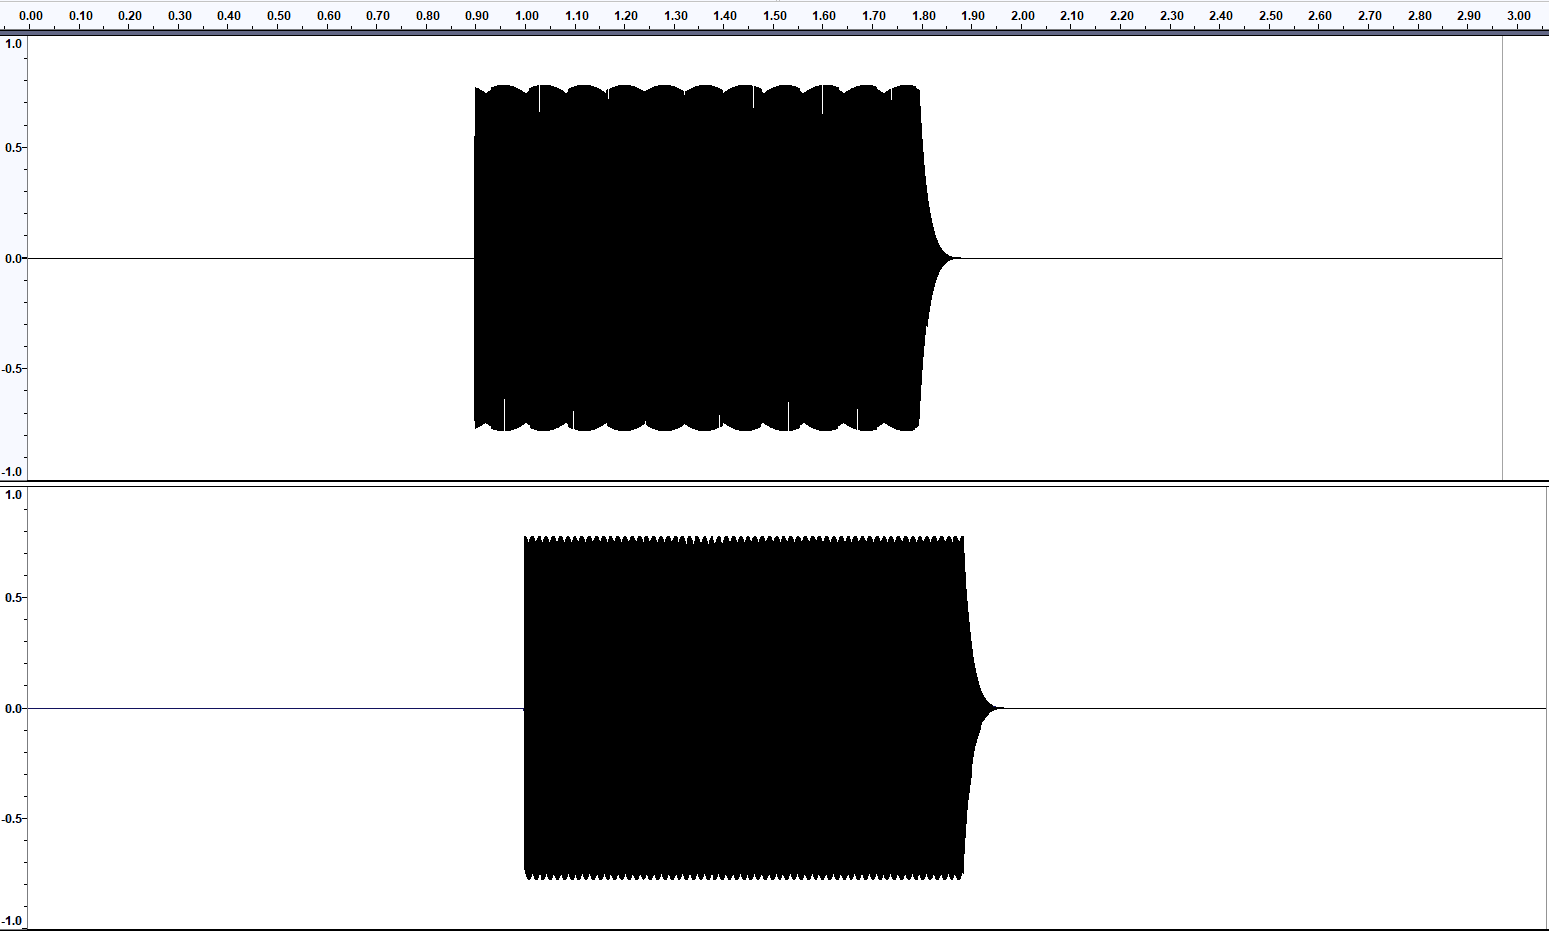
\includegraphics{images/approach-waves.png}
    \end{center}
    \caption{The output for test scene 1 for the interpolated (top) and snapshot (bottom) method, visualized using Audacity.}\label{fig:ApproachWaves}
\end{figure}

As expected and clearly visible in \autoref{fig:ApproachWaves}, the first effect can be observed in the interpolated version of the simulation,
but not in the simulation using the snapshot method.
This is because for the snapshot method,
only the initial position of the receiver is relevant to the distance a ray needs to travel until it arrives at said receiver.
Thus, the ray has to travel the full 343.2 meters for the initial impulse response, as shown in~\autoref{im:SnapshotExplain}.
The interpolated version instead takes this effect into account correctly.
\newline
One notable detail is that the interpolated method also simulates the doppler effect more accurately.
The resulting signal from the interpolated method exactly matches the \(488.\bar{8} Hz\) calculated in~\eqref{eq:Doppler},
while the snapshot method instead arrives at a frequency of approximately \(495 Hz\).
\newline
This difference in frequency can be explained by a difference in the actual travelling distance:
In the snapshot method, the receiver first receives signal after \(1s\),
with the final bit of signal arriving at \(1.9s\).
For the interpolated simulation, those numbers are \(0.9s\) and \(1.8s\) respectively.
The signal is thus heard for \(0.9s\) for both receivers.
\newline
Where the receivers' behaviour differs is in the distance they travel in the meantime:
The interpolated method's receiver first starts getting a signal after having travelled for \(34.22\) meters,
with it receiving the last signal after a \(68.44m\) travel distance,
meaning it moved for a total of \(34.22m\) over the course of receiving this signal.
Since the snapshot method doesn't take receiver movement into account,
the first signal is received after \(0m\) of travel distance,
with the final part arriving after \(38.0\bar{2}m\) of travel distance.
\newline
The difference in travel speed thus explains the difference in frequency shift,
seeing as the doppler effect directly relates to velocity.
The snapshot method's result is physically impossible:
If the frequency is shifted higher up,
the pitched-up signal would last shorter than it does with the real pitch shift.
\newline
This goes to show that the interpolated method does help to eliminate this class of error from simulation of moving scenes.
\newline
A noteworthy implementation detail becomes apparent from the waveform resulting from the simulation:
As the input signal is a single sine wave and the doppler effect would only raise its frequency,
the resulting wave should still be a pure sine wave.
In contrast, the actual result for both simulation types features aliasing effects.
\newline
This is because the simulation is run as the same sample rate as the input signal.
For each input sample, one energetic response is calculated.
As the doppler effect speeds up the incoming signal,
but the sped up signal is not upsampled accordingly,
the same effect as if the signal was downsampled and stayed at the same frequency is created.
\newline
To alleviate this, one would need to either run the signal through a low-pass filter ahead of time
or have both the input signal and simulation at a higher sample rate,
then filter and downsample to the target sample rate afterwards.
\newline
The former works, but might damage a signal more complex than a sine wave
and requires knowledge of the scene ahead of time.
For a more complex scene where the downsampling effect cannot be easily calculated prematurely,
this approach becomes unusable.
\newline
The latter leads to increased computation cost as more energetic responses need to be calculated for more signals,
but works with any arbitrary scene.

\section{Rotating Cube Scene}

\begin{table}[t!]
    \centering
    \begin{tabular}{| c | c | c | c | c | c | c |}
        \hline
        Run        & Snapshot 1 & Snapshot 2 & Snapshot 3 & Interp. 1 & Interp. 2 & Interp. 3 \\
        \hline
        Time       & 0:22:33    & 0:22:42    & 0:22:32    & 4:29:42   & 4:11:32   & 4:13:18   \\
        \hline
        \(T_{60}\) & 5.18s      & 5.18s      & 5.20s      & 5.27s     & 5.20s     & 5.18s     \\
        \hline
        \(C_{50}\) & -7.94dB    & -7.93dB    & -7.95dB    & -8.29dB   & -8.29dB   & -8.27dB   \\
        \hline
    \end{tabular}
    \caption{Rotating Cube Test Results}\label{tbl:CubeSceneTable}
\end{table}
There is very little difference in the reverberation time \(T_{60}\) between the snapshot and interpolated version of this scene.
This was to be expected:
The distance a ray has to travel to go from one end of the room to the other hardly changes between the rotating and static version of the room.
Since the angle at which a ray bounces becomes insignificant as reflections become diffuse over time,
there is no significant difference between the snapshot (static) and interpolated (non-static) version of the cube scene.
\newline
\begin{figure}[t!]
    \begin{center}
        %% Creator: Matplotlib, PGF backend
%%
%% To include the figure in your LaTeX document, write
%%   \input{<filename>.pgf}
%%
%% Make sure the required packages are loaded in your preamble
%%   \usepackage{pgf}
%%
%% Also ensure that all the required font packages are loaded; for instance,
%% the lmodern package is sometimes necessary when using math font.
%%   \usepackage{lmodern}
%%
%% Figures using additional raster images can only be included by \input if
%% they are in the same directory as the main LaTeX file. For loading figures
%% from other directories you can use the `import` package
%%   \usepackage{import}
%%
%% and then include the figures with
%%   \import{<path to file>}{<filename>.pgf}
%%
%% Matplotlib used the following preamble
%%   \def\mathdefault#1{#1}
%%   \everymath=\expandafter{\the\everymath\displaystyle}
%%   
%%   \makeatletter\@ifpackageloaded{underscore}{}{\usepackage[strings]{underscore}}\makeatother
%%
\begingroup%
\makeatletter%
\begin{pgfpicture}%
\pgfpathrectangle{\pgfpointorigin}{\pgfqpoint{6.400000in}{3.000000in}}%
\pgfusepath{use as bounding box, clip}%
\begin{pgfscope}%
\pgfsetbuttcap%
\pgfsetmiterjoin%
\definecolor{currentfill}{rgb}{1.000000,1.000000,1.000000}%
\pgfsetfillcolor{currentfill}%
\pgfsetlinewidth{0.000000pt}%
\definecolor{currentstroke}{rgb}{1.000000,1.000000,1.000000}%
\pgfsetstrokecolor{currentstroke}%
\pgfsetdash{}{0pt}%
\pgfpathmoveto{\pgfqpoint{0.000000in}{0.000000in}}%
\pgfpathlineto{\pgfqpoint{6.400000in}{0.000000in}}%
\pgfpathlineto{\pgfqpoint{6.400000in}{3.000000in}}%
\pgfpathlineto{\pgfqpoint{0.000000in}{3.000000in}}%
\pgfpathlineto{\pgfqpoint{0.000000in}{0.000000in}}%
\pgfpathclose%
\pgfusepath{fill}%
\end{pgfscope}%
\begin{pgfscope}%
\pgfsetbuttcap%
\pgfsetmiterjoin%
\definecolor{currentfill}{rgb}{1.000000,1.000000,1.000000}%
\pgfsetfillcolor{currentfill}%
\pgfsetlinewidth{0.000000pt}%
\definecolor{currentstroke}{rgb}{0.000000,0.000000,0.000000}%
\pgfsetstrokecolor{currentstroke}%
\pgfsetstrokeopacity{0.000000}%
\pgfsetdash{}{0pt}%
\pgfpathmoveto{\pgfqpoint{0.541671in}{0.441361in}}%
\pgfpathlineto{\pgfqpoint{3.019441in}{0.441361in}}%
\pgfpathlineto{\pgfqpoint{3.019441in}{2.518509in}}%
\pgfpathlineto{\pgfqpoint{0.541671in}{2.518509in}}%
\pgfpathlineto{\pgfqpoint{0.541671in}{0.441361in}}%
\pgfpathclose%
\pgfusepath{fill}%
\end{pgfscope}%
\begin{pgfscope}%
\pgfsetbuttcap%
\pgfsetroundjoin%
\definecolor{currentfill}{rgb}{0.000000,0.000000,0.000000}%
\pgfsetfillcolor{currentfill}%
\pgfsetlinewidth{0.803000pt}%
\definecolor{currentstroke}{rgb}{0.000000,0.000000,0.000000}%
\pgfsetstrokecolor{currentstroke}%
\pgfsetdash{}{0pt}%
\pgfsys@defobject{currentmarker}{\pgfqpoint{0.000000in}{-0.048611in}}{\pgfqpoint{0.000000in}{0.000000in}}{%
\pgfpathmoveto{\pgfqpoint{0.000000in}{0.000000in}}%
\pgfpathlineto{\pgfqpoint{0.000000in}{-0.048611in}}%
\pgfusepath{stroke,fill}%
}%
\begin{pgfscope}%
\pgfsys@transformshift{0.541671in}{0.441361in}%
\pgfsys@useobject{currentmarker}{}%
\end{pgfscope}%
\end{pgfscope}%
\begin{pgfscope}%
\definecolor{textcolor}{rgb}{0.000000,0.000000,0.000000}%
\pgfsetstrokecolor{textcolor}%
\pgfsetfillcolor{textcolor}%
\pgftext[x=0.541671in,y=0.344139in,,top]{\color{textcolor}{\rmfamily\fontsize{10.000000}{12.000000}\selectfont\catcode`\^=\active\def^{\ifmmode\sp\else\^{}\fi}\catcode`\%=\active\def%{\%}$\mathdefault{0}$}}%
\end{pgfscope}%
\begin{pgfscope}%
\pgfsetbuttcap%
\pgfsetroundjoin%
\definecolor{currentfill}{rgb}{0.000000,0.000000,0.000000}%
\pgfsetfillcolor{currentfill}%
\pgfsetlinewidth{0.803000pt}%
\definecolor{currentstroke}{rgb}{0.000000,0.000000,0.000000}%
\pgfsetstrokecolor{currentstroke}%
\pgfsetdash{}{0pt}%
\pgfsys@defobject{currentmarker}{\pgfqpoint{0.000000in}{-0.048611in}}{\pgfqpoint{0.000000in}{0.000000in}}{%
\pgfpathmoveto{\pgfqpoint{0.000000in}{0.000000in}}%
\pgfpathlineto{\pgfqpoint{0.000000in}{-0.048611in}}%
\pgfusepath{stroke,fill}%
}%
\begin{pgfscope}%
\pgfsys@transformshift{1.037225in}{0.441361in}%
\pgfsys@useobject{currentmarker}{}%
\end{pgfscope}%
\end{pgfscope}%
\begin{pgfscope}%
\definecolor{textcolor}{rgb}{0.000000,0.000000,0.000000}%
\pgfsetstrokecolor{textcolor}%
\pgfsetfillcolor{textcolor}%
\pgftext[x=1.037225in,y=0.344139in,,top]{\color{textcolor}{\rmfamily\fontsize{10.000000}{12.000000}\selectfont\catcode`\^=\active\def^{\ifmmode\sp\else\^{}\fi}\catcode`\%=\active\def%{\%}$\mathdefault{1000}$}}%
\end{pgfscope}%
\begin{pgfscope}%
\pgfsetbuttcap%
\pgfsetroundjoin%
\definecolor{currentfill}{rgb}{0.000000,0.000000,0.000000}%
\pgfsetfillcolor{currentfill}%
\pgfsetlinewidth{0.803000pt}%
\definecolor{currentstroke}{rgb}{0.000000,0.000000,0.000000}%
\pgfsetstrokecolor{currentstroke}%
\pgfsetdash{}{0pt}%
\pgfsys@defobject{currentmarker}{\pgfqpoint{0.000000in}{-0.048611in}}{\pgfqpoint{0.000000in}{0.000000in}}{%
\pgfpathmoveto{\pgfqpoint{0.000000in}{0.000000in}}%
\pgfpathlineto{\pgfqpoint{0.000000in}{-0.048611in}}%
\pgfusepath{stroke,fill}%
}%
\begin{pgfscope}%
\pgfsys@transformshift{1.532779in}{0.441361in}%
\pgfsys@useobject{currentmarker}{}%
\end{pgfscope}%
\end{pgfscope}%
\begin{pgfscope}%
\definecolor{textcolor}{rgb}{0.000000,0.000000,0.000000}%
\pgfsetstrokecolor{textcolor}%
\pgfsetfillcolor{textcolor}%
\pgftext[x=1.532779in,y=0.344139in,,top]{\color{textcolor}{\rmfamily\fontsize{10.000000}{12.000000}\selectfont\catcode`\^=\active\def^{\ifmmode\sp\else\^{}\fi}\catcode`\%=\active\def%{\%}$\mathdefault{2000}$}}%
\end{pgfscope}%
\begin{pgfscope}%
\pgfsetbuttcap%
\pgfsetroundjoin%
\definecolor{currentfill}{rgb}{0.000000,0.000000,0.000000}%
\pgfsetfillcolor{currentfill}%
\pgfsetlinewidth{0.803000pt}%
\definecolor{currentstroke}{rgb}{0.000000,0.000000,0.000000}%
\pgfsetstrokecolor{currentstroke}%
\pgfsetdash{}{0pt}%
\pgfsys@defobject{currentmarker}{\pgfqpoint{0.000000in}{-0.048611in}}{\pgfqpoint{0.000000in}{0.000000in}}{%
\pgfpathmoveto{\pgfqpoint{0.000000in}{0.000000in}}%
\pgfpathlineto{\pgfqpoint{0.000000in}{-0.048611in}}%
\pgfusepath{stroke,fill}%
}%
\begin{pgfscope}%
\pgfsys@transformshift{2.028333in}{0.441361in}%
\pgfsys@useobject{currentmarker}{}%
\end{pgfscope}%
\end{pgfscope}%
\begin{pgfscope}%
\definecolor{textcolor}{rgb}{0.000000,0.000000,0.000000}%
\pgfsetstrokecolor{textcolor}%
\pgfsetfillcolor{textcolor}%
\pgftext[x=2.028333in,y=0.344139in,,top]{\color{textcolor}{\rmfamily\fontsize{10.000000}{12.000000}\selectfont\catcode`\^=\active\def^{\ifmmode\sp\else\^{}\fi}\catcode`\%=\active\def%{\%}$\mathdefault{3000}$}}%
\end{pgfscope}%
\begin{pgfscope}%
\pgfsetbuttcap%
\pgfsetroundjoin%
\definecolor{currentfill}{rgb}{0.000000,0.000000,0.000000}%
\pgfsetfillcolor{currentfill}%
\pgfsetlinewidth{0.803000pt}%
\definecolor{currentstroke}{rgb}{0.000000,0.000000,0.000000}%
\pgfsetstrokecolor{currentstroke}%
\pgfsetdash{}{0pt}%
\pgfsys@defobject{currentmarker}{\pgfqpoint{0.000000in}{-0.048611in}}{\pgfqpoint{0.000000in}{0.000000in}}{%
\pgfpathmoveto{\pgfqpoint{0.000000in}{0.000000in}}%
\pgfpathlineto{\pgfqpoint{0.000000in}{-0.048611in}}%
\pgfusepath{stroke,fill}%
}%
\begin{pgfscope}%
\pgfsys@transformshift{2.523887in}{0.441361in}%
\pgfsys@useobject{currentmarker}{}%
\end{pgfscope}%
\end{pgfscope}%
\begin{pgfscope}%
\definecolor{textcolor}{rgb}{0.000000,0.000000,0.000000}%
\pgfsetstrokecolor{textcolor}%
\pgfsetfillcolor{textcolor}%
\pgftext[x=2.523887in,y=0.344139in,,top]{\color{textcolor}{\rmfamily\fontsize{10.000000}{12.000000}\selectfont\catcode`\^=\active\def^{\ifmmode\sp\else\^{}\fi}\catcode`\%=\active\def%{\%}$\mathdefault{4000}$}}%
\end{pgfscope}%
\begin{pgfscope}%
\pgfsetbuttcap%
\pgfsetroundjoin%
\definecolor{currentfill}{rgb}{0.000000,0.000000,0.000000}%
\pgfsetfillcolor{currentfill}%
\pgfsetlinewidth{0.803000pt}%
\definecolor{currentstroke}{rgb}{0.000000,0.000000,0.000000}%
\pgfsetstrokecolor{currentstroke}%
\pgfsetdash{}{0pt}%
\pgfsys@defobject{currentmarker}{\pgfqpoint{0.000000in}{-0.048611in}}{\pgfqpoint{0.000000in}{0.000000in}}{%
\pgfpathmoveto{\pgfqpoint{0.000000in}{0.000000in}}%
\pgfpathlineto{\pgfqpoint{0.000000in}{-0.048611in}}%
\pgfusepath{stroke,fill}%
}%
\begin{pgfscope}%
\pgfsys@transformshift{3.019441in}{0.441361in}%
\pgfsys@useobject{currentmarker}{}%
\end{pgfscope}%
\end{pgfscope}%
\begin{pgfscope}%
\definecolor{textcolor}{rgb}{0.000000,0.000000,0.000000}%
\pgfsetstrokecolor{textcolor}%
\pgfsetfillcolor{textcolor}%
\pgftext[x=3.019441in,y=0.344139in,,top]{\color{textcolor}{\rmfamily\fontsize{10.000000}{12.000000}\selectfont\catcode`\^=\active\def^{\ifmmode\sp\else\^{}\fi}\catcode`\%=\active\def%{\%}$\mathdefault{5000}$}}%
\end{pgfscope}%
\begin{pgfscope}%
\definecolor{textcolor}{rgb}{0.000000,0.000000,0.000000}%
\pgfsetstrokecolor{textcolor}%
\pgfsetfillcolor{textcolor}%
\pgftext[x=1.780556in,y=0.165127in,,top]{\color{textcolor}{\rmfamily\fontsize{10.000000}{12.000000}\selectfont\catcode`\^=\active\def^{\ifmmode\sp\else\^{}\fi}\catcode`\%=\active\def%{\%}Sample}}%
\end{pgfscope}%
\begin{pgfscope}%
\pgfsetbuttcap%
\pgfsetroundjoin%
\definecolor{currentfill}{rgb}{0.000000,0.000000,0.000000}%
\pgfsetfillcolor{currentfill}%
\pgfsetlinewidth{0.803000pt}%
\definecolor{currentstroke}{rgb}{0.000000,0.000000,0.000000}%
\pgfsetstrokecolor{currentstroke}%
\pgfsetdash{}{0pt}%
\pgfsys@defobject{currentmarker}{\pgfqpoint{-0.048611in}{0.000000in}}{\pgfqpoint{-0.000000in}{0.000000in}}{%
\pgfpathmoveto{\pgfqpoint{-0.000000in}{0.000000in}}%
\pgfpathlineto{\pgfqpoint{-0.048611in}{0.000000in}}%
\pgfusepath{stroke,fill}%
}%
\begin{pgfscope}%
\pgfsys@transformshift{0.541671in}{0.441361in}%
\pgfsys@useobject{currentmarker}{}%
\end{pgfscope}%
\end{pgfscope}%
\begin{pgfscope}%
\definecolor{textcolor}{rgb}{0.000000,0.000000,0.000000}%
\pgfsetstrokecolor{textcolor}%
\pgfsetfillcolor{textcolor}%
\pgftext[x=0.375004in, y=0.393136in, left, base]{\color{textcolor}{\rmfamily\fontsize{10.000000}{12.000000}\selectfont\catcode`\^=\active\def^{\ifmmode\sp\else\^{}\fi}\catcode`\%=\active\def%{\%}$\mathdefault{0}$}}%
\end{pgfscope}%
\begin{pgfscope}%
\pgfsetbuttcap%
\pgfsetroundjoin%
\definecolor{currentfill}{rgb}{0.000000,0.000000,0.000000}%
\pgfsetfillcolor{currentfill}%
\pgfsetlinewidth{0.803000pt}%
\definecolor{currentstroke}{rgb}{0.000000,0.000000,0.000000}%
\pgfsetstrokecolor{currentstroke}%
\pgfsetdash{}{0pt}%
\pgfsys@defobject{currentmarker}{\pgfqpoint{-0.048611in}{0.000000in}}{\pgfqpoint{-0.000000in}{0.000000in}}{%
\pgfpathmoveto{\pgfqpoint{-0.000000in}{0.000000in}}%
\pgfpathlineto{\pgfqpoint{-0.048611in}{0.000000in}}%
\pgfusepath{stroke,fill}%
}%
\begin{pgfscope}%
\pgfsys@transformshift{0.541671in}{0.837008in}%
\pgfsys@useobject{currentmarker}{}%
\end{pgfscope}%
\end{pgfscope}%
\begin{pgfscope}%
\definecolor{textcolor}{rgb}{0.000000,0.000000,0.000000}%
\pgfsetstrokecolor{textcolor}%
\pgfsetfillcolor{textcolor}%
\pgftext[x=0.305559in, y=0.788783in, left, base]{\color{textcolor}{\rmfamily\fontsize{10.000000}{12.000000}\selectfont\catcode`\^=\active\def^{\ifmmode\sp\else\^{}\fi}\catcode`\%=\active\def%{\%}$\mathdefault{20}$}}%
\end{pgfscope}%
\begin{pgfscope}%
\pgfsetbuttcap%
\pgfsetroundjoin%
\definecolor{currentfill}{rgb}{0.000000,0.000000,0.000000}%
\pgfsetfillcolor{currentfill}%
\pgfsetlinewidth{0.803000pt}%
\definecolor{currentstroke}{rgb}{0.000000,0.000000,0.000000}%
\pgfsetstrokecolor{currentstroke}%
\pgfsetdash{}{0pt}%
\pgfsys@defobject{currentmarker}{\pgfqpoint{-0.048611in}{0.000000in}}{\pgfqpoint{-0.000000in}{0.000000in}}{%
\pgfpathmoveto{\pgfqpoint{-0.000000in}{0.000000in}}%
\pgfpathlineto{\pgfqpoint{-0.048611in}{0.000000in}}%
\pgfusepath{stroke,fill}%
}%
\begin{pgfscope}%
\pgfsys@transformshift{0.541671in}{1.232656in}%
\pgfsys@useobject{currentmarker}{}%
\end{pgfscope}%
\end{pgfscope}%
\begin{pgfscope}%
\definecolor{textcolor}{rgb}{0.000000,0.000000,0.000000}%
\pgfsetstrokecolor{textcolor}%
\pgfsetfillcolor{textcolor}%
\pgftext[x=0.305559in, y=1.184430in, left, base]{\color{textcolor}{\rmfamily\fontsize{10.000000}{12.000000}\selectfont\catcode`\^=\active\def^{\ifmmode\sp\else\^{}\fi}\catcode`\%=\active\def%{\%}$\mathdefault{40}$}}%
\end{pgfscope}%
\begin{pgfscope}%
\pgfsetbuttcap%
\pgfsetroundjoin%
\definecolor{currentfill}{rgb}{0.000000,0.000000,0.000000}%
\pgfsetfillcolor{currentfill}%
\pgfsetlinewidth{0.803000pt}%
\definecolor{currentstroke}{rgb}{0.000000,0.000000,0.000000}%
\pgfsetstrokecolor{currentstroke}%
\pgfsetdash{}{0pt}%
\pgfsys@defobject{currentmarker}{\pgfqpoint{-0.048611in}{0.000000in}}{\pgfqpoint{-0.000000in}{0.000000in}}{%
\pgfpathmoveto{\pgfqpoint{-0.000000in}{0.000000in}}%
\pgfpathlineto{\pgfqpoint{-0.048611in}{0.000000in}}%
\pgfusepath{stroke,fill}%
}%
\begin{pgfscope}%
\pgfsys@transformshift{0.541671in}{1.628303in}%
\pgfsys@useobject{currentmarker}{}%
\end{pgfscope}%
\end{pgfscope}%
\begin{pgfscope}%
\definecolor{textcolor}{rgb}{0.000000,0.000000,0.000000}%
\pgfsetstrokecolor{textcolor}%
\pgfsetfillcolor{textcolor}%
\pgftext[x=0.305559in, y=1.580078in, left, base]{\color{textcolor}{\rmfamily\fontsize{10.000000}{12.000000}\selectfont\catcode`\^=\active\def^{\ifmmode\sp\else\^{}\fi}\catcode`\%=\active\def%{\%}$\mathdefault{60}$}}%
\end{pgfscope}%
\begin{pgfscope}%
\pgfsetbuttcap%
\pgfsetroundjoin%
\definecolor{currentfill}{rgb}{0.000000,0.000000,0.000000}%
\pgfsetfillcolor{currentfill}%
\pgfsetlinewidth{0.803000pt}%
\definecolor{currentstroke}{rgb}{0.000000,0.000000,0.000000}%
\pgfsetstrokecolor{currentstroke}%
\pgfsetdash{}{0pt}%
\pgfsys@defobject{currentmarker}{\pgfqpoint{-0.048611in}{0.000000in}}{\pgfqpoint{-0.000000in}{0.000000in}}{%
\pgfpathmoveto{\pgfqpoint{-0.000000in}{0.000000in}}%
\pgfpathlineto{\pgfqpoint{-0.048611in}{0.000000in}}%
\pgfusepath{stroke,fill}%
}%
\begin{pgfscope}%
\pgfsys@transformshift{0.541671in}{2.023950in}%
\pgfsys@useobject{currentmarker}{}%
\end{pgfscope}%
\end{pgfscope}%
\begin{pgfscope}%
\definecolor{textcolor}{rgb}{0.000000,0.000000,0.000000}%
\pgfsetstrokecolor{textcolor}%
\pgfsetfillcolor{textcolor}%
\pgftext[x=0.305559in, y=1.975725in, left, base]{\color{textcolor}{\rmfamily\fontsize{10.000000}{12.000000}\selectfont\catcode`\^=\active\def^{\ifmmode\sp\else\^{}\fi}\catcode`\%=\active\def%{\%}$\mathdefault{80}$}}%
\end{pgfscope}%
\begin{pgfscope}%
\pgfsetbuttcap%
\pgfsetroundjoin%
\definecolor{currentfill}{rgb}{0.000000,0.000000,0.000000}%
\pgfsetfillcolor{currentfill}%
\pgfsetlinewidth{0.803000pt}%
\definecolor{currentstroke}{rgb}{0.000000,0.000000,0.000000}%
\pgfsetstrokecolor{currentstroke}%
\pgfsetdash{}{0pt}%
\pgfsys@defobject{currentmarker}{\pgfqpoint{-0.048611in}{0.000000in}}{\pgfqpoint{-0.000000in}{0.000000in}}{%
\pgfpathmoveto{\pgfqpoint{-0.000000in}{0.000000in}}%
\pgfpathlineto{\pgfqpoint{-0.048611in}{0.000000in}}%
\pgfusepath{stroke,fill}%
}%
\begin{pgfscope}%
\pgfsys@transformshift{0.541671in}{2.419597in}%
\pgfsys@useobject{currentmarker}{}%
\end{pgfscope}%
\end{pgfscope}%
\begin{pgfscope}%
\definecolor{textcolor}{rgb}{0.000000,0.000000,0.000000}%
\pgfsetstrokecolor{textcolor}%
\pgfsetfillcolor{textcolor}%
\pgftext[x=0.236114in, y=2.371372in, left, base]{\color{textcolor}{\rmfamily\fontsize{10.000000}{12.000000}\selectfont\catcode`\^=\active\def^{\ifmmode\sp\else\^{}\fi}\catcode`\%=\active\def%{\%}$\mathdefault{100}$}}%
\end{pgfscope}%
\begin{pgfscope}%
\definecolor{textcolor}{rgb}{0.000000,0.000000,0.000000}%
\pgfsetstrokecolor{textcolor}%
\pgfsetfillcolor{textcolor}%
\pgftext[x=0.180559in,y=1.479935in,,bottom,rotate=90.000000]{\color{textcolor}{\rmfamily\fontsize{10.000000}{12.000000}\selectfont\catcode`\^=\active\def^{\ifmmode\sp\else\^{}\fi}\catcode`\%=\active\def%{\%}Energy (% of maximum)}}%
\end{pgfscope}%
\begin{pgfscope}%
\pgfpathrectangle{\pgfqpoint{0.541671in}{0.441361in}}{\pgfqpoint{2.477770in}{2.077148in}}%
\pgfusepath{clip}%
\pgfsetrectcap%
\pgfsetroundjoin%
\pgfsetlinewidth{1.505625pt}%
\definecolor{currentstroke}{rgb}{0.121569,0.466667,0.705882}%
\pgfsetstrokecolor{currentstroke}%
\pgfsetdash{}{0pt}%
\pgfpathmoveto{\pgfqpoint{0.541671in}{0.441361in}}%
\pgfpathlineto{\pgfqpoint{0.611048in}{0.441361in}}%
\pgfpathlineto{\pgfqpoint{0.611544in}{0.810445in}}%
\pgfpathlineto{\pgfqpoint{0.612039in}{2.419597in}}%
\pgfpathlineto{\pgfqpoint{0.613030in}{2.054707in}}%
\pgfpathlineto{\pgfqpoint{0.617986in}{0.446953in}}%
\pgfpathlineto{\pgfqpoint{0.619473in}{0.441361in}}%
\pgfpathlineto{\pgfqpoint{0.649206in}{0.441361in}}%
\pgfpathlineto{\pgfqpoint{0.649701in}{0.496165in}}%
\pgfpathlineto{\pgfqpoint{0.650197in}{1.185318in}}%
\pgfpathlineto{\pgfqpoint{0.651188in}{1.138735in}}%
\pgfpathlineto{\pgfqpoint{0.656639in}{0.448212in}}%
\pgfpathlineto{\pgfqpoint{0.657135in}{0.448212in}}%
\pgfpathlineto{\pgfqpoint{0.659117in}{0.461912in}}%
\pgfpathlineto{\pgfqpoint{0.659613in}{0.445471in}}%
\pgfpathlineto{\pgfqpoint{0.660108in}{0.457802in}}%
\pgfpathlineto{\pgfqpoint{0.662090in}{0.449582in}}%
\pgfpathlineto{\pgfqpoint{0.662586in}{0.457802in}}%
\pgfpathlineto{\pgfqpoint{0.663081in}{0.449582in}}%
\pgfpathlineto{\pgfqpoint{0.664073in}{0.463282in}}%
\pgfpathlineto{\pgfqpoint{0.664568in}{0.457802in}}%
\pgfpathlineto{\pgfqpoint{0.665559in}{0.450952in}}%
\pgfpathlineto{\pgfqpoint{0.666055in}{0.455062in}}%
\pgfpathlineto{\pgfqpoint{0.666550in}{0.456432in}}%
\pgfpathlineto{\pgfqpoint{0.667046in}{0.448212in}}%
\pgfpathlineto{\pgfqpoint{0.667541in}{0.455062in}}%
\pgfpathlineto{\pgfqpoint{0.668037in}{0.450952in}}%
\pgfpathlineto{\pgfqpoint{0.668533in}{0.452322in}}%
\pgfpathlineto{\pgfqpoint{0.669028in}{0.460542in}}%
\pgfpathlineto{\pgfqpoint{0.669524in}{0.445471in}}%
\pgfpathlineto{\pgfqpoint{0.670019in}{0.448212in}}%
\pgfpathlineto{\pgfqpoint{0.670515in}{0.449582in}}%
\pgfpathlineto{\pgfqpoint{0.671010in}{0.448212in}}%
\pgfpathlineto{\pgfqpoint{0.672497in}{0.445471in}}%
\pgfpathlineto{\pgfqpoint{0.673984in}{0.450952in}}%
\pgfpathlineto{\pgfqpoint{0.674975in}{0.445471in}}%
\pgfpathlineto{\pgfqpoint{0.675470in}{0.452322in}}%
\pgfpathlineto{\pgfqpoint{0.676461in}{0.450952in}}%
\pgfpathlineto{\pgfqpoint{0.676957in}{0.444101in}}%
\pgfpathlineto{\pgfqpoint{0.677452in}{0.445471in}}%
\pgfpathlineto{\pgfqpoint{0.677948in}{0.449582in}}%
\pgfpathlineto{\pgfqpoint{0.678444in}{0.445471in}}%
\pgfpathlineto{\pgfqpoint{0.678939in}{0.445471in}}%
\pgfpathlineto{\pgfqpoint{0.679930in}{0.446841in}}%
\pgfpathlineto{\pgfqpoint{0.681417in}{0.442731in}}%
\pgfpathlineto{\pgfqpoint{0.681912in}{0.446841in}}%
\pgfpathlineto{\pgfqpoint{0.682408in}{0.442731in}}%
\pgfpathlineto{\pgfqpoint{0.683895in}{0.442731in}}%
\pgfpathlineto{\pgfqpoint{0.685381in}{0.446841in}}%
\pgfpathlineto{\pgfqpoint{0.685877in}{0.446841in}}%
\pgfpathlineto{\pgfqpoint{0.687364in}{0.441361in}}%
\pgfpathlineto{\pgfqpoint{0.689346in}{0.445471in}}%
\pgfpathlineto{\pgfqpoint{0.690832in}{0.442731in}}%
\pgfpathlineto{\pgfqpoint{0.691824in}{0.441361in}}%
\pgfpathlineto{\pgfqpoint{0.692319in}{0.448212in}}%
\pgfpathlineto{\pgfqpoint{0.692815in}{0.441361in}}%
\pgfpathlineto{\pgfqpoint{0.693806in}{0.445471in}}%
\pgfpathlineto{\pgfqpoint{0.694797in}{0.442731in}}%
\pgfpathlineto{\pgfqpoint{0.695292in}{0.445471in}}%
\pgfpathlineto{\pgfqpoint{0.696779in}{0.441361in}}%
\pgfpathlineto{\pgfqpoint{0.697275in}{0.444101in}}%
\pgfpathlineto{\pgfqpoint{0.697770in}{0.442731in}}%
\pgfpathlineto{\pgfqpoint{0.699257in}{0.441361in}}%
\pgfpathlineto{\pgfqpoint{0.700248in}{0.444101in}}%
\pgfpathlineto{\pgfqpoint{0.700744in}{0.442731in}}%
\pgfpathlineto{\pgfqpoint{0.701239in}{0.442731in}}%
\pgfpathlineto{\pgfqpoint{0.702230in}{0.441361in}}%
\pgfpathlineto{\pgfqpoint{0.702726in}{0.444101in}}%
\pgfpathlineto{\pgfqpoint{0.703221in}{0.442731in}}%
\pgfpathlineto{\pgfqpoint{0.703717in}{0.442731in}}%
\pgfpathlineto{\pgfqpoint{0.705204in}{0.441361in}}%
\pgfpathlineto{\pgfqpoint{0.705699in}{0.441361in}}%
\pgfpathlineto{\pgfqpoint{0.707186in}{0.445471in}}%
\pgfpathlineto{\pgfqpoint{0.708672in}{0.441361in}}%
\pgfpathlineto{\pgfqpoint{0.709168in}{0.441361in}}%
\pgfpathlineto{\pgfqpoint{0.710159in}{0.445471in}}%
\pgfpathlineto{\pgfqpoint{0.711150in}{0.441361in}}%
\pgfpathlineto{\pgfqpoint{0.712141in}{0.442731in}}%
\pgfpathlineto{\pgfqpoint{0.712637in}{0.441361in}}%
\pgfpathlineto{\pgfqpoint{0.714123in}{0.444101in}}%
\pgfpathlineto{\pgfqpoint{0.715610in}{0.441361in}}%
\pgfpathlineto{\pgfqpoint{0.716601in}{0.444101in}}%
\pgfpathlineto{\pgfqpoint{0.717592in}{0.441361in}}%
\pgfpathlineto{\pgfqpoint{0.719079in}{0.444101in}}%
\pgfpathlineto{\pgfqpoint{0.720566in}{0.441361in}}%
\pgfpathlineto{\pgfqpoint{0.721557in}{0.442731in}}%
\pgfpathlineto{\pgfqpoint{0.722052in}{0.441361in}}%
\pgfpathlineto{\pgfqpoint{0.723043in}{0.444101in}}%
\pgfpathlineto{\pgfqpoint{0.724530in}{0.441361in}}%
\pgfpathlineto{\pgfqpoint{0.726017in}{0.442731in}}%
\pgfpathlineto{\pgfqpoint{0.727008in}{0.442731in}}%
\pgfpathlineto{\pgfqpoint{0.727999in}{0.441361in}}%
\pgfpathlineto{\pgfqpoint{0.728495in}{0.444101in}}%
\pgfpathlineto{\pgfqpoint{0.728990in}{0.441361in}}%
\pgfpathlineto{\pgfqpoint{0.729981in}{0.441361in}}%
\pgfpathlineto{\pgfqpoint{0.730477in}{0.442731in}}%
\pgfpathlineto{\pgfqpoint{0.730972in}{0.441361in}}%
\pgfpathlineto{\pgfqpoint{0.731468in}{0.441361in}}%
\pgfpathlineto{\pgfqpoint{0.733450in}{0.444101in}}%
\pgfpathlineto{\pgfqpoint{0.733946in}{0.444101in}}%
\pgfpathlineto{\pgfqpoint{0.734441in}{0.441361in}}%
\pgfpathlineto{\pgfqpoint{0.734937in}{0.442731in}}%
\pgfpathlineto{\pgfqpoint{0.735432in}{0.444101in}}%
\pgfpathlineto{\pgfqpoint{0.736919in}{0.441361in}}%
\pgfpathlineto{\pgfqpoint{0.738406in}{0.445471in}}%
\pgfpathlineto{\pgfqpoint{0.739892in}{0.441361in}}%
\pgfpathlineto{\pgfqpoint{0.741379in}{0.442731in}}%
\pgfpathlineto{\pgfqpoint{0.741875in}{0.442731in}}%
\pgfpathlineto{\pgfqpoint{0.743361in}{0.441361in}}%
\pgfpathlineto{\pgfqpoint{0.743857in}{0.441361in}}%
\pgfpathlineto{\pgfqpoint{0.744352in}{0.442731in}}%
\pgfpathlineto{\pgfqpoint{0.744848in}{0.441361in}}%
\pgfpathlineto{\pgfqpoint{0.747821in}{0.441361in}}%
\pgfpathlineto{\pgfqpoint{0.748317in}{0.444101in}}%
\pgfpathlineto{\pgfqpoint{0.748812in}{0.442731in}}%
\pgfpathlineto{\pgfqpoint{0.749308in}{0.441361in}}%
\pgfpathlineto{\pgfqpoint{0.749803in}{0.444101in}}%
\pgfpathlineto{\pgfqpoint{0.750299in}{0.441361in}}%
\pgfpathlineto{\pgfqpoint{0.751290in}{0.442731in}}%
\pgfpathlineto{\pgfqpoint{0.751786in}{0.441361in}}%
\pgfpathlineto{\pgfqpoint{0.752281in}{0.442731in}}%
\pgfpathlineto{\pgfqpoint{0.752777in}{0.445471in}}%
\pgfpathlineto{\pgfqpoint{0.754263in}{0.441361in}}%
\pgfpathlineto{\pgfqpoint{0.754759in}{0.442731in}}%
\pgfpathlineto{\pgfqpoint{0.755254in}{0.441361in}}%
\pgfpathlineto{\pgfqpoint{0.757237in}{0.441361in}}%
\pgfpathlineto{\pgfqpoint{0.757732in}{0.442731in}}%
\pgfpathlineto{\pgfqpoint{0.758228in}{0.441361in}}%
\pgfpathlineto{\pgfqpoint{0.758723in}{0.441361in}}%
\pgfpathlineto{\pgfqpoint{0.760210in}{0.444101in}}%
\pgfpathlineto{\pgfqpoint{0.761201in}{0.441361in}}%
\pgfpathlineto{\pgfqpoint{0.763183in}{0.444101in}}%
\pgfpathlineto{\pgfqpoint{0.764670in}{0.441361in}}%
\pgfpathlineto{\pgfqpoint{0.765661in}{0.441361in}}%
\pgfpathlineto{\pgfqpoint{0.766157in}{0.442731in}}%
\pgfpathlineto{\pgfqpoint{0.766652in}{0.441361in}}%
\pgfpathlineto{\pgfqpoint{0.767148in}{0.441361in}}%
\pgfpathlineto{\pgfqpoint{0.768634in}{0.442731in}}%
\pgfpathlineto{\pgfqpoint{0.770121in}{0.441361in}}%
\pgfpathlineto{\pgfqpoint{0.771112in}{0.441361in}}%
\pgfpathlineto{\pgfqpoint{0.771608in}{0.442731in}}%
\pgfpathlineto{\pgfqpoint{0.772103in}{0.441361in}}%
\pgfpathlineto{\pgfqpoint{0.775077in}{0.441361in}}%
\pgfpathlineto{\pgfqpoint{0.775572in}{0.442731in}}%
\pgfpathlineto{\pgfqpoint{0.776068in}{0.441361in}}%
\pgfpathlineto{\pgfqpoint{0.779537in}{0.441361in}}%
\pgfpathlineto{\pgfqpoint{0.781023in}{0.442731in}}%
\pgfpathlineto{\pgfqpoint{0.781519in}{0.442731in}}%
\pgfpathlineto{\pgfqpoint{0.783005in}{0.441361in}}%
\pgfpathlineto{\pgfqpoint{0.784492in}{0.444101in}}%
\pgfpathlineto{\pgfqpoint{0.785483in}{0.441361in}}%
\pgfpathlineto{\pgfqpoint{0.786970in}{0.442731in}}%
\pgfpathlineto{\pgfqpoint{0.787961in}{0.441361in}}%
\pgfpathlineto{\pgfqpoint{0.788457in}{0.445471in}}%
\pgfpathlineto{\pgfqpoint{0.788952in}{0.441361in}}%
\pgfpathlineto{\pgfqpoint{0.797377in}{0.441361in}}%
\pgfpathlineto{\pgfqpoint{0.798863in}{0.442731in}}%
\pgfpathlineto{\pgfqpoint{0.800350in}{0.441361in}}%
\pgfpathlineto{\pgfqpoint{0.800845in}{0.441361in}}%
\pgfpathlineto{\pgfqpoint{0.801837in}{1.048309in}}%
\pgfpathlineto{\pgfqpoint{0.802332in}{0.994876in}}%
\pgfpathlineto{\pgfqpoint{0.803323in}{1.067490in}}%
\pgfpathlineto{\pgfqpoint{0.806297in}{0.607142in}}%
\pgfpathlineto{\pgfqpoint{0.809270in}{0.444101in}}%
\pgfpathlineto{\pgfqpoint{0.809765in}{0.446841in}}%
\pgfpathlineto{\pgfqpoint{0.810261in}{0.445471in}}%
\pgfpathlineto{\pgfqpoint{0.811748in}{0.441361in}}%
\pgfpathlineto{\pgfqpoint{0.813234in}{0.446841in}}%
\pgfpathlineto{\pgfqpoint{0.814225in}{0.442731in}}%
\pgfpathlineto{\pgfqpoint{0.815217in}{1.012002in}}%
\pgfpathlineto{\pgfqpoint{0.815712in}{0.954266in}}%
\pgfpathlineto{\pgfqpoint{0.816208in}{0.928783in}}%
\pgfpathlineto{\pgfqpoint{0.818190in}{0.742122in}}%
\pgfpathlineto{\pgfqpoint{0.820668in}{0.491177in}}%
\pgfpathlineto{\pgfqpoint{0.821163in}{0.450870in}}%
\pgfpathlineto{\pgfqpoint{0.822154in}{0.457583in}}%
\pgfpathlineto{\pgfqpoint{0.823145in}{0.449499in}}%
\pgfpathlineto{\pgfqpoint{0.823641in}{0.452212in}}%
\pgfpathlineto{\pgfqpoint{0.824632in}{0.456185in}}%
\pgfpathlineto{\pgfqpoint{0.826119in}{0.445417in}}%
\pgfpathlineto{\pgfqpoint{0.827110in}{0.460268in}}%
\pgfpathlineto{\pgfqpoint{0.827605in}{0.450815in}}%
\pgfpathlineto{\pgfqpoint{0.828596in}{0.458898in}}%
\pgfpathlineto{\pgfqpoint{0.829092in}{0.453446in}}%
\pgfpathlineto{\pgfqpoint{0.829588in}{0.448075in}}%
\pgfpathlineto{\pgfqpoint{0.830083in}{0.452157in}}%
\pgfpathlineto{\pgfqpoint{0.830579in}{0.457556in}}%
\pgfpathlineto{\pgfqpoint{0.831074in}{0.454815in}}%
\pgfpathlineto{\pgfqpoint{0.832065in}{0.449472in}}%
\pgfpathlineto{\pgfqpoint{0.833056in}{0.456159in}}%
\pgfpathlineto{\pgfqpoint{0.833552in}{0.453500in}}%
\pgfpathlineto{\pgfqpoint{0.834048in}{0.448130in}}%
\pgfpathlineto{\pgfqpoint{0.834543in}{0.452185in}}%
\pgfpathlineto{\pgfqpoint{0.835534in}{0.453582in}}%
\pgfpathlineto{\pgfqpoint{0.836525in}{0.446732in}}%
\pgfpathlineto{\pgfqpoint{0.837021in}{0.450815in}}%
\pgfpathlineto{\pgfqpoint{0.837516in}{0.449445in}}%
\pgfpathlineto{\pgfqpoint{0.838508in}{0.449445in}}%
\pgfpathlineto{\pgfqpoint{0.839003in}{0.445417in}}%
\pgfpathlineto{\pgfqpoint{0.840490in}{0.450815in}}%
\pgfpathlineto{\pgfqpoint{0.841481in}{0.530060in}}%
\pgfpathlineto{\pgfqpoint{0.841976in}{0.511235in}}%
\pgfpathlineto{\pgfqpoint{0.842472in}{0.529951in}}%
\pgfpathlineto{\pgfqpoint{0.842968in}{0.495096in}}%
\pgfpathlineto{\pgfqpoint{0.843463in}{0.511236in}}%
\pgfpathlineto{\pgfqpoint{0.844950in}{0.491151in}}%
\pgfpathlineto{\pgfqpoint{0.847428in}{0.453446in}}%
\pgfpathlineto{\pgfqpoint{0.847923in}{0.450870in}}%
\pgfpathlineto{\pgfqpoint{0.848419in}{0.452158in}}%
\pgfpathlineto{\pgfqpoint{0.849410in}{0.453529in}}%
\pgfpathlineto{\pgfqpoint{0.849905in}{0.452157in}}%
\pgfpathlineto{\pgfqpoint{0.850401in}{0.454843in}}%
\pgfpathlineto{\pgfqpoint{0.850896in}{0.452240in}}%
\pgfpathlineto{\pgfqpoint{0.851887in}{0.452131in}}%
\pgfpathlineto{\pgfqpoint{0.852879in}{0.454898in}}%
\pgfpathlineto{\pgfqpoint{0.853374in}{0.454790in}}%
\pgfpathlineto{\pgfqpoint{0.853870in}{0.454789in}}%
\pgfpathlineto{\pgfqpoint{0.855356in}{0.446759in}}%
\pgfpathlineto{\pgfqpoint{0.855852in}{0.453527in}}%
\pgfpathlineto{\pgfqpoint{0.856347in}{0.448075in}}%
\pgfpathlineto{\pgfqpoint{0.857834in}{0.452185in}}%
\pgfpathlineto{\pgfqpoint{0.858330in}{0.450788in}}%
\pgfpathlineto{\pgfqpoint{0.858825in}{0.454816in}}%
\pgfpathlineto{\pgfqpoint{0.859321in}{0.452076in}}%
\pgfpathlineto{\pgfqpoint{0.860312in}{0.444074in}}%
\pgfpathlineto{\pgfqpoint{0.860807in}{0.446841in}}%
\pgfpathlineto{\pgfqpoint{0.861799in}{0.453500in}}%
\pgfpathlineto{\pgfqpoint{0.862294in}{0.445389in}}%
\pgfpathlineto{\pgfqpoint{0.862790in}{0.450842in}}%
\pgfpathlineto{\pgfqpoint{0.864276in}{0.452157in}}%
\pgfpathlineto{\pgfqpoint{0.864772in}{0.452130in}}%
\pgfpathlineto{\pgfqpoint{0.865763in}{0.446705in}}%
\pgfpathlineto{\pgfqpoint{0.866259in}{0.448075in}}%
\pgfpathlineto{\pgfqpoint{0.866754in}{0.452158in}}%
\pgfpathlineto{\pgfqpoint{0.867745in}{0.444046in}}%
\pgfpathlineto{\pgfqpoint{0.869232in}{0.453501in}}%
\pgfpathlineto{\pgfqpoint{0.869727in}{0.446706in}}%
\pgfpathlineto{\pgfqpoint{0.870223in}{0.450707in}}%
\pgfpathlineto{\pgfqpoint{0.871214in}{0.453529in}}%
\pgfpathlineto{\pgfqpoint{0.872205in}{0.445389in}}%
\pgfpathlineto{\pgfqpoint{0.873196in}{0.453446in}}%
\pgfpathlineto{\pgfqpoint{0.873692in}{0.449472in}}%
\pgfpathlineto{\pgfqpoint{0.874187in}{0.452185in}}%
\pgfpathlineto{\pgfqpoint{0.875674in}{0.446760in}}%
\pgfpathlineto{\pgfqpoint{0.876665in}{0.450843in}}%
\pgfpathlineto{\pgfqpoint{0.877161in}{0.446732in}}%
\pgfpathlineto{\pgfqpoint{0.878647in}{0.457475in}}%
\pgfpathlineto{\pgfqpoint{0.879143in}{0.447968in}}%
\pgfpathlineto{\pgfqpoint{0.880134in}{0.448157in}}%
\pgfpathlineto{\pgfqpoint{0.881621in}{0.444074in}}%
\pgfpathlineto{\pgfqpoint{0.883107in}{0.453501in}}%
\pgfpathlineto{\pgfqpoint{0.884099in}{0.448102in}}%
\pgfpathlineto{\pgfqpoint{0.884594in}{0.449527in}}%
\pgfpathlineto{\pgfqpoint{0.885090in}{0.453419in}}%
\pgfpathlineto{\pgfqpoint{0.886081in}{0.446787in}}%
\pgfpathlineto{\pgfqpoint{0.887567in}{0.450843in}}%
\pgfpathlineto{\pgfqpoint{0.888063in}{0.445390in}}%
\pgfpathlineto{\pgfqpoint{0.888558in}{0.446787in}}%
\pgfpathlineto{\pgfqpoint{0.889550in}{0.452212in}}%
\pgfpathlineto{\pgfqpoint{0.890541in}{0.444046in}}%
\pgfpathlineto{\pgfqpoint{0.891036in}{0.453527in}}%
\pgfpathlineto{\pgfqpoint{0.892027in}{0.452157in}}%
\pgfpathlineto{\pgfqpoint{0.893514in}{0.449500in}}%
\pgfpathlineto{\pgfqpoint{0.894010in}{0.452049in}}%
\pgfpathlineto{\pgfqpoint{0.894505in}{0.450843in}}%
\pgfpathlineto{\pgfqpoint{0.895001in}{0.445417in}}%
\pgfpathlineto{\pgfqpoint{0.895496in}{0.449499in}}%
\pgfpathlineto{\pgfqpoint{0.895992in}{0.449472in}}%
\pgfpathlineto{\pgfqpoint{0.896983in}{0.453474in}}%
\pgfpathlineto{\pgfqpoint{0.897478in}{0.448129in}}%
\pgfpathlineto{\pgfqpoint{0.898470in}{0.449473in}}%
\pgfpathlineto{\pgfqpoint{0.899461in}{0.448129in}}%
\pgfpathlineto{\pgfqpoint{0.899956in}{0.453555in}}%
\pgfpathlineto{\pgfqpoint{0.900452in}{0.450815in}}%
\pgfpathlineto{\pgfqpoint{0.901443in}{0.446705in}}%
\pgfpathlineto{\pgfqpoint{0.901938in}{0.442731in}}%
\pgfpathlineto{\pgfqpoint{0.902434in}{0.456240in}}%
\pgfpathlineto{\pgfqpoint{0.902930in}{0.445417in}}%
\pgfpathlineto{\pgfqpoint{0.904912in}{1.708882in}}%
\pgfpathlineto{\pgfqpoint{0.905903in}{1.518221in}}%
\pgfpathlineto{\pgfqpoint{0.910363in}{0.523239in}}%
\pgfpathlineto{\pgfqpoint{0.911850in}{0.464269in}}%
\pgfpathlineto{\pgfqpoint{0.912841in}{0.457473in}}%
\pgfpathlineto{\pgfqpoint{0.913832in}{1.117886in}}%
\pgfpathlineto{\pgfqpoint{0.914327in}{1.074626in}}%
\pgfpathlineto{\pgfqpoint{0.916310in}{0.869356in}}%
\pgfpathlineto{\pgfqpoint{0.919778in}{0.470417in}}%
\pgfpathlineto{\pgfqpoint{0.920274in}{0.477372in}}%
\pgfpathlineto{\pgfqpoint{0.920770in}{0.470578in}}%
\pgfpathlineto{\pgfqpoint{0.921761in}{0.465261in}}%
\pgfpathlineto{\pgfqpoint{0.923247in}{0.470632in}}%
\pgfpathlineto{\pgfqpoint{0.924238in}{0.461314in}}%
\pgfpathlineto{\pgfqpoint{0.924734in}{0.471840in}}%
\pgfpathlineto{\pgfqpoint{0.925229in}{0.466524in}}%
\pgfpathlineto{\pgfqpoint{0.925725in}{0.466525in}}%
\pgfpathlineto{\pgfqpoint{0.926221in}{0.459784in}}%
\pgfpathlineto{\pgfqpoint{0.926716in}{0.470473in}}%
\pgfpathlineto{\pgfqpoint{0.927212in}{0.463811in}}%
\pgfpathlineto{\pgfqpoint{0.927707in}{0.466364in}}%
\pgfpathlineto{\pgfqpoint{0.928203in}{0.477025in}}%
\pgfpathlineto{\pgfqpoint{0.928698in}{0.467920in}}%
\pgfpathlineto{\pgfqpoint{0.929194in}{0.470473in}}%
\pgfpathlineto{\pgfqpoint{0.930681in}{0.462603in}}%
\pgfpathlineto{\pgfqpoint{0.931176in}{0.465343in}}%
\pgfpathlineto{\pgfqpoint{0.931672in}{0.462550in}}%
\pgfpathlineto{\pgfqpoint{0.932167in}{0.457233in}}%
\pgfpathlineto{\pgfqpoint{0.932663in}{0.467841in}}%
\pgfpathlineto{\pgfqpoint{0.933654in}{0.870430in}}%
\pgfpathlineto{\pgfqpoint{0.934645in}{0.824349in}}%
\pgfpathlineto{\pgfqpoint{0.937618in}{0.598000in}}%
\pgfpathlineto{\pgfqpoint{0.939105in}{0.497943in}}%
\pgfpathlineto{\pgfqpoint{0.939601in}{0.463893in}}%
\pgfpathlineto{\pgfqpoint{0.940592in}{0.466471in}}%
\pgfpathlineto{\pgfqpoint{0.941087in}{0.461152in}}%
\pgfpathlineto{\pgfqpoint{0.941583in}{0.475655in}}%
\pgfpathlineto{\pgfqpoint{0.942078in}{0.467786in}}%
\pgfpathlineto{\pgfqpoint{0.942574in}{0.467733in}}%
\pgfpathlineto{\pgfqpoint{0.943069in}{0.458495in}}%
\pgfpathlineto{\pgfqpoint{0.943565in}{0.469103in}}%
\pgfpathlineto{\pgfqpoint{0.944061in}{0.463705in}}%
\pgfpathlineto{\pgfqpoint{0.945547in}{0.482371in}}%
\pgfpathlineto{\pgfqpoint{0.947034in}{0.459891in}}%
\pgfpathlineto{\pgfqpoint{0.948025in}{0.474420in}}%
\pgfpathlineto{\pgfqpoint{0.949016in}{0.462577in}}%
\pgfpathlineto{\pgfqpoint{0.949512in}{0.467707in}}%
\pgfpathlineto{\pgfqpoint{0.950007in}{0.467840in}}%
\pgfpathlineto{\pgfqpoint{0.950503in}{0.459733in}}%
\pgfpathlineto{\pgfqpoint{0.950998in}{0.465101in}}%
\pgfpathlineto{\pgfqpoint{0.951989in}{0.463761in}}%
\pgfpathlineto{\pgfqpoint{0.952485in}{0.465154in}}%
\pgfpathlineto{\pgfqpoint{0.952981in}{0.474313in}}%
\pgfpathlineto{\pgfqpoint{0.953972in}{0.458442in}}%
\pgfpathlineto{\pgfqpoint{0.954467in}{0.461207in}}%
\pgfpathlineto{\pgfqpoint{0.954963in}{0.469156in}}%
\pgfpathlineto{\pgfqpoint{0.955458in}{0.462444in}}%
\pgfpathlineto{\pgfqpoint{0.955954in}{0.463972in}}%
\pgfpathlineto{\pgfqpoint{0.956945in}{0.459838in}}%
\pgfpathlineto{\pgfqpoint{0.957936in}{0.462550in}}%
\pgfpathlineto{\pgfqpoint{0.958432in}{0.461153in}}%
\pgfpathlineto{\pgfqpoint{0.958927in}{0.462443in}}%
\pgfpathlineto{\pgfqpoint{0.960414in}{0.469156in}}%
\pgfpathlineto{\pgfqpoint{0.961900in}{0.454574in}}%
\pgfpathlineto{\pgfqpoint{0.962396in}{0.455864in}}%
\pgfpathlineto{\pgfqpoint{0.963387in}{0.454681in}}%
\pgfpathlineto{\pgfqpoint{0.963883in}{0.467680in}}%
\pgfpathlineto{\pgfqpoint{0.964378in}{0.469128in}}%
\pgfpathlineto{\pgfqpoint{0.965369in}{0.455864in}}%
\pgfpathlineto{\pgfqpoint{0.965865in}{0.457232in}}%
\pgfpathlineto{\pgfqpoint{0.966360in}{0.449310in}}%
\pgfpathlineto{\pgfqpoint{0.967847in}{0.459972in}}%
\pgfpathlineto{\pgfqpoint{0.968343in}{0.463919in}}%
\pgfpathlineto{\pgfqpoint{0.968838in}{0.455889in}}%
\pgfpathlineto{\pgfqpoint{0.969334in}{0.455944in}}%
\pgfpathlineto{\pgfqpoint{0.969829in}{0.461127in}}%
\pgfpathlineto{\pgfqpoint{0.970325in}{0.455838in}}%
\pgfpathlineto{\pgfqpoint{0.971316in}{0.453231in}}%
\pgfpathlineto{\pgfqpoint{0.972307in}{0.467734in}}%
\pgfpathlineto{\pgfqpoint{0.973298in}{0.459918in}}%
\pgfpathlineto{\pgfqpoint{0.974289in}{0.462522in}}%
\pgfpathlineto{\pgfqpoint{0.975280in}{0.453205in}}%
\pgfpathlineto{\pgfqpoint{0.975776in}{0.461075in}}%
\pgfpathlineto{\pgfqpoint{0.976272in}{0.457206in}}%
\pgfpathlineto{\pgfqpoint{0.976767in}{0.451889in}}%
\pgfpathlineto{\pgfqpoint{0.977263in}{0.453205in}}%
\pgfpathlineto{\pgfqpoint{0.978254in}{0.459784in}}%
\pgfpathlineto{\pgfqpoint{0.980236in}{0.447995in}}%
\pgfpathlineto{\pgfqpoint{0.980732in}{0.449310in}}%
\pgfpathlineto{\pgfqpoint{0.981723in}{0.462284in}}%
\pgfpathlineto{\pgfqpoint{0.982218in}{0.453285in}}%
\pgfpathlineto{\pgfqpoint{0.983209in}{0.454628in}}%
\pgfpathlineto{\pgfqpoint{0.983705in}{0.471626in}}%
\pgfpathlineto{\pgfqpoint{0.984200in}{1.146807in}}%
\pgfpathlineto{\pgfqpoint{0.985192in}{1.097909in}}%
\pgfpathlineto{\pgfqpoint{0.987174in}{0.818952in}}%
\pgfpathlineto{\pgfqpoint{0.990643in}{0.459705in}}%
\pgfpathlineto{\pgfqpoint{0.992129in}{0.461073in}}%
\pgfpathlineto{\pgfqpoint{0.992625in}{0.457100in}}%
\pgfpathlineto{\pgfqpoint{0.993120in}{0.461153in}}%
\pgfpathlineto{\pgfqpoint{0.993616in}{0.463919in}}%
\pgfpathlineto{\pgfqpoint{0.995103in}{0.507855in}}%
\pgfpathlineto{\pgfqpoint{0.995598in}{0.490638in}}%
\pgfpathlineto{\pgfqpoint{0.996589in}{0.491981in}}%
\pgfpathlineto{\pgfqpoint{0.997085in}{0.490745in}}%
\pgfpathlineto{\pgfqpoint{0.997580in}{0.462683in}}%
\pgfpathlineto{\pgfqpoint{0.998076in}{0.473292in}}%
\pgfpathlineto{\pgfqpoint{0.998571in}{0.480656in}}%
\pgfpathlineto{\pgfqpoint{1.000058in}{0.449257in}}%
\pgfpathlineto{\pgfqpoint{1.000554in}{0.466310in}}%
\pgfpathlineto{\pgfqpoint{1.001049in}{0.450599in}}%
\pgfpathlineto{\pgfqpoint{1.003031in}{0.462363in}}%
\pgfpathlineto{\pgfqpoint{1.003527in}{0.459784in}}%
\pgfpathlineto{\pgfqpoint{1.004023in}{0.458469in}}%
\pgfpathlineto{\pgfqpoint{1.004518in}{0.459652in}}%
\pgfpathlineto{\pgfqpoint{1.005509in}{0.462391in}}%
\pgfpathlineto{\pgfqpoint{1.006005in}{0.455783in}}%
\pgfpathlineto{\pgfqpoint{1.006500in}{0.466205in}}%
\pgfpathlineto{\pgfqpoint{1.006996in}{0.453126in}}%
\pgfpathlineto{\pgfqpoint{1.007491in}{0.478915in}}%
\pgfpathlineto{\pgfqpoint{1.007987in}{0.913773in}}%
\pgfpathlineto{\pgfqpoint{1.008978in}{0.855639in}}%
\pgfpathlineto{\pgfqpoint{1.012447in}{0.571786in}}%
\pgfpathlineto{\pgfqpoint{1.015916in}{0.454388in}}%
\pgfpathlineto{\pgfqpoint{1.017403in}{0.480337in}}%
\pgfpathlineto{\pgfqpoint{1.018394in}{0.458283in}}%
\pgfpathlineto{\pgfqpoint{1.018889in}{0.464704in}}%
\pgfpathlineto{\pgfqpoint{1.019385in}{0.458309in}}%
\pgfpathlineto{\pgfqpoint{1.020376in}{0.470154in}}%
\pgfpathlineto{\pgfqpoint{1.020871in}{0.453019in}}%
\pgfpathlineto{\pgfqpoint{1.021367in}{0.460969in}}%
\pgfpathlineto{\pgfqpoint{1.022358in}{0.470075in}}%
\pgfpathlineto{\pgfqpoint{1.022854in}{0.456967in}}%
\pgfpathlineto{\pgfqpoint{1.023349in}{0.459573in}}%
\pgfpathlineto{\pgfqpoint{1.023845in}{0.464678in}}%
\pgfpathlineto{\pgfqpoint{1.024340in}{0.458283in}}%
\pgfpathlineto{\pgfqpoint{1.024836in}{0.466047in}}%
\pgfpathlineto{\pgfqpoint{1.025331in}{0.458469in}}%
\pgfpathlineto{\pgfqpoint{1.025827in}{0.466127in}}%
\pgfpathlineto{\pgfqpoint{1.026323in}{0.458311in}}%
\pgfpathlineto{\pgfqpoint{1.027314in}{0.466075in}}%
\pgfpathlineto{\pgfqpoint{1.028800in}{0.453021in}}%
\pgfpathlineto{\pgfqpoint{1.029296in}{0.464704in}}%
\pgfpathlineto{\pgfqpoint{1.029791in}{0.454389in}}%
\pgfpathlineto{\pgfqpoint{1.030287in}{0.453125in}}%
\pgfpathlineto{\pgfqpoint{1.033260in}{0.493706in}}%
\pgfpathlineto{\pgfqpoint{1.034747in}{0.474047in}}%
\pgfpathlineto{\pgfqpoint{1.035242in}{0.473943in}}%
\pgfpathlineto{\pgfqpoint{1.036729in}{0.455652in}}%
\pgfpathlineto{\pgfqpoint{1.037225in}{0.461047in}}%
\pgfpathlineto{\pgfqpoint{1.037720in}{0.466100in}}%
\pgfpathlineto{\pgfqpoint{1.038216in}{0.466021in}}%
\pgfpathlineto{\pgfqpoint{1.039207in}{0.456889in}}%
\pgfpathlineto{\pgfqpoint{1.039702in}{0.462231in}}%
\pgfpathlineto{\pgfqpoint{1.040198in}{0.456968in}}%
\pgfpathlineto{\pgfqpoint{1.041685in}{0.453125in}}%
\pgfpathlineto{\pgfqpoint{1.042676in}{0.458100in}}%
\pgfpathlineto{\pgfqpoint{1.043171in}{0.454389in}}%
\pgfpathlineto{\pgfqpoint{1.043667in}{0.457046in}}%
\pgfpathlineto{\pgfqpoint{1.044162in}{0.462204in}}%
\pgfpathlineto{\pgfqpoint{1.045154in}{0.450495in}}%
\pgfpathlineto{\pgfqpoint{1.046145in}{0.463521in}}%
\pgfpathlineto{\pgfqpoint{1.046640in}{0.463470in}}%
\pgfpathlineto{\pgfqpoint{1.047136in}{0.460996in}}%
\pgfpathlineto{\pgfqpoint{1.047631in}{0.451809in}}%
\pgfpathlineto{\pgfqpoint{1.048127in}{0.459547in}}%
\pgfpathlineto{\pgfqpoint{1.048622in}{0.459678in}}%
\pgfpathlineto{\pgfqpoint{1.049118in}{0.455626in}}%
\pgfpathlineto{\pgfqpoint{1.049614in}{0.462154in}}%
\pgfpathlineto{\pgfqpoint{1.050109in}{0.450493in}}%
\pgfpathlineto{\pgfqpoint{1.051100in}{0.584497in}}%
\pgfpathlineto{\pgfqpoint{1.051596in}{0.576176in}}%
\pgfpathlineto{\pgfqpoint{1.052091in}{0.541614in}}%
\pgfpathlineto{\pgfqpoint{1.053082in}{0.541636in}}%
\pgfpathlineto{\pgfqpoint{1.053578in}{0.539085in}}%
\pgfpathlineto{\pgfqpoint{1.056551in}{0.455866in}}%
\pgfpathlineto{\pgfqpoint{1.057047in}{0.451730in}}%
\pgfpathlineto{\pgfqpoint{1.058534in}{0.562366in}}%
\pgfpathlineto{\pgfqpoint{1.059525in}{0.559603in}}%
\pgfpathlineto{\pgfqpoint{1.060020in}{0.708345in}}%
\pgfpathlineto{\pgfqpoint{1.060516in}{0.662343in}}%
\pgfpathlineto{\pgfqpoint{1.061011in}{0.670159in}}%
\pgfpathlineto{\pgfqpoint{1.063985in}{0.530627in}}%
\pgfpathlineto{\pgfqpoint{1.065967in}{0.464863in}}%
\pgfpathlineto{\pgfqpoint{1.066462in}{0.451731in}}%
\pgfpathlineto{\pgfqpoint{1.066958in}{0.458285in}}%
\pgfpathlineto{\pgfqpoint{1.067453in}{0.456996in}}%
\pgfpathlineto{\pgfqpoint{1.067949in}{0.449151in}}%
\pgfpathlineto{\pgfqpoint{1.068445in}{0.457126in}}%
\pgfpathlineto{\pgfqpoint{1.069436in}{0.451836in}}%
\pgfpathlineto{\pgfqpoint{1.069931in}{0.453073in}}%
\pgfpathlineto{\pgfqpoint{1.070427in}{0.458207in}}%
\pgfpathlineto{\pgfqpoint{1.070922in}{0.454468in}}%
\pgfpathlineto{\pgfqpoint{1.071418in}{0.451653in}}%
\pgfpathlineto{\pgfqpoint{1.071913in}{0.455652in}}%
\pgfpathlineto{\pgfqpoint{1.072409in}{0.447889in}}%
\pgfpathlineto{\pgfqpoint{1.072905in}{0.455810in}}%
\pgfpathlineto{\pgfqpoint{1.073400in}{0.451809in}}%
\pgfpathlineto{\pgfqpoint{1.073896in}{0.453048in}}%
\pgfpathlineto{\pgfqpoint{1.074391in}{0.460996in}}%
\pgfpathlineto{\pgfqpoint{1.074887in}{0.455811in}}%
\pgfpathlineto{\pgfqpoint{1.076373in}{0.451782in}}%
\pgfpathlineto{\pgfqpoint{1.076869in}{0.453178in}}%
\pgfpathlineto{\pgfqpoint{1.077365in}{0.463389in}}%
\pgfpathlineto{\pgfqpoint{1.077860in}{0.455731in}}%
\pgfpathlineto{\pgfqpoint{1.078356in}{0.449179in}}%
\pgfpathlineto{\pgfqpoint{1.078851in}{0.454336in}}%
\pgfpathlineto{\pgfqpoint{1.079347in}{0.462127in}}%
\pgfpathlineto{\pgfqpoint{1.080833in}{0.446546in}}%
\pgfpathlineto{\pgfqpoint{1.081329in}{0.454468in}}%
\pgfpathlineto{\pgfqpoint{1.081825in}{0.453099in}}%
\pgfpathlineto{\pgfqpoint{1.082320in}{0.449125in}}%
\pgfpathlineto{\pgfqpoint{1.082816in}{0.458206in}}%
\pgfpathlineto{\pgfqpoint{1.083311in}{0.449283in}}%
\pgfpathlineto{\pgfqpoint{1.084302in}{0.457021in}}%
\pgfpathlineto{\pgfqpoint{1.084798in}{0.455626in}}%
\pgfpathlineto{\pgfqpoint{1.085293in}{0.457021in}}%
\pgfpathlineto{\pgfqpoint{1.086285in}{0.447861in}}%
\pgfpathlineto{\pgfqpoint{1.086780in}{0.455652in}}%
\pgfpathlineto{\pgfqpoint{1.087276in}{0.446624in}}%
\pgfpathlineto{\pgfqpoint{1.088267in}{0.456916in}}%
\pgfpathlineto{\pgfqpoint{1.088762in}{0.451863in}}%
\pgfpathlineto{\pgfqpoint{1.089753in}{0.451809in}}%
\pgfpathlineto{\pgfqpoint{1.090249in}{0.462207in}}%
\pgfpathlineto{\pgfqpoint{1.090745in}{0.459626in}}%
\pgfpathlineto{\pgfqpoint{1.091240in}{0.447863in}}%
\pgfpathlineto{\pgfqpoint{1.091736in}{0.449231in}}%
\pgfpathlineto{\pgfqpoint{1.093222in}{0.459574in}}%
\pgfpathlineto{\pgfqpoint{1.094213in}{0.578183in}}%
\pgfpathlineto{\pgfqpoint{1.096196in}{0.514866in}}%
\pgfpathlineto{\pgfqpoint{1.096691in}{0.521338in}}%
\pgfpathlineto{\pgfqpoint{1.099169in}{0.463548in}}%
\pgfpathlineto{\pgfqpoint{1.100656in}{0.451809in}}%
\pgfpathlineto{\pgfqpoint{1.101151in}{0.452970in}}%
\pgfpathlineto{\pgfqpoint{1.101647in}{0.458232in}}%
\pgfpathlineto{\pgfqpoint{1.102142in}{0.453048in}}%
\pgfpathlineto{\pgfqpoint{1.103133in}{0.451730in}}%
\pgfpathlineto{\pgfqpoint{1.103629in}{0.456967in}}%
\pgfpathlineto{\pgfqpoint{1.104124in}{0.454258in}}%
\pgfpathlineto{\pgfqpoint{1.105116in}{0.450520in}}%
\pgfpathlineto{\pgfqpoint{1.105611in}{0.451836in}}%
\pgfpathlineto{\pgfqpoint{1.107098in}{0.463468in}}%
\pgfpathlineto{\pgfqpoint{1.107593in}{0.447835in}}%
\pgfpathlineto{\pgfqpoint{1.108089in}{0.452941in}}%
\pgfpathlineto{\pgfqpoint{1.108584in}{0.455678in}}%
\pgfpathlineto{\pgfqpoint{1.109080in}{0.449257in}}%
\pgfpathlineto{\pgfqpoint{1.109576in}{0.462257in}}%
\pgfpathlineto{\pgfqpoint{1.111062in}{0.837243in}}%
\pgfpathlineto{\pgfqpoint{1.112549in}{0.686028in}}%
\pgfpathlineto{\pgfqpoint{1.113044in}{0.739924in}}%
\pgfpathlineto{\pgfqpoint{1.114531in}{0.575394in}}%
\pgfpathlineto{\pgfqpoint{1.115522in}{0.526706in}}%
\pgfpathlineto{\pgfqpoint{1.116018in}{0.492547in}}%
\pgfpathlineto{\pgfqpoint{1.116513in}{0.693161in}}%
\pgfpathlineto{\pgfqpoint{1.117504in}{0.677633in}}%
\pgfpathlineto{\pgfqpoint{1.118000in}{0.643921in}}%
\pgfpathlineto{\pgfqpoint{1.118991in}{0.757373in}}%
\pgfpathlineto{\pgfqpoint{1.119487in}{0.741898in}}%
\pgfpathlineto{\pgfqpoint{1.122956in}{0.529286in}}%
\pgfpathlineto{\pgfqpoint{1.124938in}{0.459495in}}%
\pgfpathlineto{\pgfqpoint{1.125433in}{0.460731in}}%
\pgfpathlineto{\pgfqpoint{1.126920in}{0.471075in}}%
\pgfpathlineto{\pgfqpoint{1.127416in}{0.458205in}}%
\pgfpathlineto{\pgfqpoint{1.127911in}{0.465915in}}%
\pgfpathlineto{\pgfqpoint{1.128407in}{0.467337in}}%
\pgfpathlineto{\pgfqpoint{1.128902in}{0.460757in}}%
\pgfpathlineto{\pgfqpoint{1.130389in}{0.587157in}}%
\pgfpathlineto{\pgfqpoint{1.130884in}{0.580999in}}%
\pgfpathlineto{\pgfqpoint{1.132867in}{0.514969in}}%
\pgfpathlineto{\pgfqpoint{1.133362in}{0.516312in}}%
\pgfpathlineto{\pgfqpoint{1.134849in}{0.487785in}}%
\pgfpathlineto{\pgfqpoint{1.136335in}{0.454336in}}%
\pgfpathlineto{\pgfqpoint{1.136831in}{0.455547in}}%
\pgfpathlineto{\pgfqpoint{1.137327in}{0.468547in}}%
\pgfpathlineto{\pgfqpoint{1.137822in}{0.467179in}}%
\pgfpathlineto{\pgfqpoint{1.138318in}{0.456863in}}%
\pgfpathlineto{\pgfqpoint{1.138813in}{0.467283in}}%
\pgfpathlineto{\pgfqpoint{1.139309in}{0.468444in}}%
\pgfpathlineto{\pgfqpoint{1.139804in}{0.453020in}}%
\pgfpathlineto{\pgfqpoint{1.140300in}{0.463389in}}%
\pgfpathlineto{\pgfqpoint{1.140795in}{0.456968in}}%
\pgfpathlineto{\pgfqpoint{1.141291in}{0.462126in}}%
\pgfpathlineto{\pgfqpoint{1.142282in}{0.456863in}}%
\pgfpathlineto{\pgfqpoint{1.143273in}{0.469759in}}%
\pgfpathlineto{\pgfqpoint{1.143769in}{0.464704in}}%
\pgfpathlineto{\pgfqpoint{1.144760in}{0.456864in}}%
\pgfpathlineto{\pgfqpoint{1.145751in}{0.459416in}}%
\pgfpathlineto{\pgfqpoint{1.146742in}{0.456811in}}%
\pgfpathlineto{\pgfqpoint{1.147238in}{0.463338in}}%
\pgfpathlineto{\pgfqpoint{1.147733in}{0.455651in}}%
\pgfpathlineto{\pgfqpoint{1.148229in}{0.458205in}}%
\pgfpathlineto{\pgfqpoint{1.148724in}{0.482214in}}%
\pgfpathlineto{\pgfqpoint{1.149715in}{0.593501in}}%
\pgfpathlineto{\pgfqpoint{1.150211in}{0.566911in}}%
\pgfpathlineto{\pgfqpoint{1.152689in}{0.506252in}}%
\pgfpathlineto{\pgfqpoint{1.153184in}{0.516387in}}%
\pgfpathlineto{\pgfqpoint{1.155167in}{0.463311in}}%
\pgfpathlineto{\pgfqpoint{1.155662in}{0.472287in}}%
\pgfpathlineto{\pgfqpoint{1.157149in}{0.461995in}}%
\pgfpathlineto{\pgfqpoint{1.157644in}{0.467128in}}%
\pgfpathlineto{\pgfqpoint{1.158140in}{0.456732in}}%
\pgfpathlineto{\pgfqpoint{1.158635in}{0.461892in}}%
\pgfpathlineto{\pgfqpoint{1.159131in}{0.462021in}}%
\pgfpathlineto{\pgfqpoint{1.159627in}{0.456784in}}%
\pgfpathlineto{\pgfqpoint{1.160122in}{0.465762in}}%
\pgfpathlineto{\pgfqpoint{1.160618in}{0.462021in}}%
\pgfpathlineto{\pgfqpoint{1.161113in}{0.462074in}}%
\pgfpathlineto{\pgfqpoint{1.161609in}{0.465812in}}%
\pgfpathlineto{\pgfqpoint{1.162600in}{0.467025in}}%
\pgfpathlineto{\pgfqpoint{1.163095in}{0.460706in}}%
\pgfpathlineto{\pgfqpoint{1.164087in}{0.465917in}}%
\pgfpathlineto{\pgfqpoint{1.165573in}{0.713322in}}%
\pgfpathlineto{\pgfqpoint{1.168051in}{0.588264in}}%
\pgfpathlineto{\pgfqpoint{1.168547in}{0.577950in}}%
\pgfpathlineto{\pgfqpoint{1.170529in}{0.479816in}}%
\pgfpathlineto{\pgfqpoint{1.172511in}{0.455469in}}%
\pgfpathlineto{\pgfqpoint{1.173006in}{0.465891in}}%
\pgfpathlineto{\pgfqpoint{1.173502in}{0.456811in}}%
\pgfpathlineto{\pgfqpoint{1.173998in}{0.455573in}}%
\pgfpathlineto{\pgfqpoint{1.175484in}{0.464575in}}%
\pgfpathlineto{\pgfqpoint{1.176475in}{0.458074in}}%
\pgfpathlineto{\pgfqpoint{1.177962in}{0.469655in}}%
\pgfpathlineto{\pgfqpoint{1.178458in}{0.455573in}}%
\pgfpathlineto{\pgfqpoint{1.178953in}{0.472157in}}%
\pgfpathlineto{\pgfqpoint{1.180935in}{0.454233in}}%
\pgfpathlineto{\pgfqpoint{1.181431in}{0.456759in}}%
\pgfpathlineto{\pgfqpoint{1.181926in}{0.693283in}}%
\pgfpathlineto{\pgfqpoint{1.182918in}{0.675537in}}%
\pgfpathlineto{\pgfqpoint{1.184404in}{0.609675in}}%
\pgfpathlineto{\pgfqpoint{1.184900in}{0.606659in}}%
\pgfpathlineto{\pgfqpoint{1.188369in}{0.479978in}}%
\pgfpathlineto{\pgfqpoint{1.189855in}{0.466947in}}%
\pgfpathlineto{\pgfqpoint{1.190351in}{0.472158in}}%
\pgfpathlineto{\pgfqpoint{1.190846in}{0.465682in}}%
\pgfpathlineto{\pgfqpoint{1.192829in}{0.471897in}}%
\pgfpathlineto{\pgfqpoint{1.194315in}{0.461788in}}%
\pgfpathlineto{\pgfqpoint{1.195306in}{0.472079in}}%
\pgfpathlineto{\pgfqpoint{1.195802in}{0.461787in}}%
\pgfpathlineto{\pgfqpoint{1.196793in}{0.463181in}}%
\pgfpathlineto{\pgfqpoint{1.197289in}{0.462847in}}%
\pgfpathlineto{\pgfqpoint{1.198280in}{0.468312in}}%
\pgfpathlineto{\pgfqpoint{1.198775in}{0.454154in}}%
\pgfpathlineto{\pgfqpoint{1.199271in}{0.467130in}}%
\pgfpathlineto{\pgfqpoint{1.201253in}{0.456785in}}%
\pgfpathlineto{\pgfqpoint{1.201749in}{0.464214in}}%
\pgfpathlineto{\pgfqpoint{1.202244in}{0.458024in}}%
\pgfpathlineto{\pgfqpoint{1.202740in}{0.460474in}}%
\pgfpathlineto{\pgfqpoint{1.203235in}{0.470635in}}%
\pgfpathlineto{\pgfqpoint{1.203731in}{0.468184in}}%
\pgfpathlineto{\pgfqpoint{1.204722in}{0.461918in}}%
\pgfpathlineto{\pgfqpoint{1.205218in}{0.463233in}}%
\pgfpathlineto{\pgfqpoint{1.205713in}{0.468109in}}%
\pgfpathlineto{\pgfqpoint{1.206704in}{0.460498in}}%
\pgfpathlineto{\pgfqpoint{1.207200in}{0.461841in}}%
\pgfpathlineto{\pgfqpoint{1.208191in}{0.466998in}}%
\pgfpathlineto{\pgfqpoint{1.208686in}{0.456682in}}%
\pgfpathlineto{\pgfqpoint{1.209182in}{0.461891in}}%
\pgfpathlineto{\pgfqpoint{1.209677in}{0.465580in}}%
\pgfpathlineto{\pgfqpoint{1.210173in}{0.478351in}}%
\pgfpathlineto{\pgfqpoint{1.211164in}{0.461557in}}%
\pgfpathlineto{\pgfqpoint{1.211660in}{0.470609in}}%
\pgfpathlineto{\pgfqpoint{1.212155in}{0.466769in}}%
\pgfpathlineto{\pgfqpoint{1.212651in}{0.467024in}}%
\pgfpathlineto{\pgfqpoint{1.214137in}{0.461608in}}%
\pgfpathlineto{\pgfqpoint{1.214633in}{0.475793in}}%
\pgfpathlineto{\pgfqpoint{1.215129in}{0.466895in}}%
\pgfpathlineto{\pgfqpoint{1.218102in}{0.460422in}}%
\pgfpathlineto{\pgfqpoint{1.220084in}{0.468132in}}%
\pgfpathlineto{\pgfqpoint{1.220580in}{0.499107in}}%
\pgfpathlineto{\pgfqpoint{1.221075in}{0.602294in}}%
\pgfpathlineto{\pgfqpoint{1.222066in}{0.589271in}}%
\pgfpathlineto{\pgfqpoint{1.224049in}{0.543053in}}%
\pgfpathlineto{\pgfqpoint{1.224544in}{0.536607in}}%
\pgfpathlineto{\pgfqpoint{1.226526in}{0.478553in}}%
\pgfpathlineto{\pgfqpoint{1.228013in}{0.457921in}}%
\pgfpathlineto{\pgfqpoint{1.229004in}{0.473138in}}%
\pgfpathlineto{\pgfqpoint{1.229500in}{0.456733in}}%
\pgfpathlineto{\pgfqpoint{1.229995in}{0.461790in}}%
\pgfpathlineto{\pgfqpoint{1.230491in}{0.461943in}}%
\pgfpathlineto{\pgfqpoint{1.230986in}{0.457945in}}%
\pgfpathlineto{\pgfqpoint{1.232969in}{0.488816in}}%
\pgfpathlineto{\pgfqpoint{1.233464in}{0.531399in}}%
\pgfpathlineto{\pgfqpoint{1.233960in}{0.528896in}}%
\pgfpathlineto{\pgfqpoint{1.235446in}{0.501713in}}%
\pgfpathlineto{\pgfqpoint{1.236933in}{0.510868in}}%
\pgfpathlineto{\pgfqpoint{1.238420in}{0.468159in}}%
\pgfpathlineto{\pgfqpoint{1.238915in}{0.475537in}}%
\pgfpathlineto{\pgfqpoint{1.239411in}{0.459339in}}%
\pgfpathlineto{\pgfqpoint{1.240402in}{0.460398in}}%
\pgfpathlineto{\pgfqpoint{1.240897in}{0.457945in}}%
\pgfpathlineto{\pgfqpoint{1.241393in}{0.459286in}}%
\pgfpathlineto{\pgfqpoint{1.241888in}{0.466742in}}%
\pgfpathlineto{\pgfqpoint{1.242384in}{0.461840in}}%
\pgfpathlineto{\pgfqpoint{1.243375in}{0.468262in}}%
\pgfpathlineto{\pgfqpoint{1.243871in}{0.456632in}}%
\pgfpathlineto{\pgfqpoint{1.244366in}{0.465579in}}%
\pgfpathlineto{\pgfqpoint{1.245357in}{0.459108in}}%
\pgfpathlineto{\pgfqpoint{1.245853in}{0.460576in}}%
\pgfpathlineto{\pgfqpoint{1.246348in}{0.465686in}}%
\pgfpathlineto{\pgfqpoint{1.247340in}{0.607040in}}%
\pgfpathlineto{\pgfqpoint{1.247835in}{0.586743in}}%
\pgfpathlineto{\pgfqpoint{1.249817in}{0.533743in}}%
\pgfpathlineto{\pgfqpoint{1.250313in}{0.538747in}}%
\pgfpathlineto{\pgfqpoint{1.252791in}{0.468006in}}%
\pgfpathlineto{\pgfqpoint{1.254773in}{0.456604in}}%
\pgfpathlineto{\pgfqpoint{1.255764in}{0.468056in}}%
\pgfpathlineto{\pgfqpoint{1.257251in}{0.460551in}}%
\pgfpathlineto{\pgfqpoint{1.257746in}{0.469218in}}%
\pgfpathlineto{\pgfqpoint{1.258242in}{0.465451in}}%
\pgfpathlineto{\pgfqpoint{1.258737in}{0.456528in}}%
\pgfpathlineto{\pgfqpoint{1.259233in}{0.462872in}}%
\pgfpathlineto{\pgfqpoint{1.260224in}{0.625401in}}%
\pgfpathlineto{\pgfqpoint{1.261215in}{0.586692in}}%
\pgfpathlineto{\pgfqpoint{1.264188in}{0.507954in}}%
\pgfpathlineto{\pgfqpoint{1.264684in}{0.525491in}}%
\pgfpathlineto{\pgfqpoint{1.265180in}{0.603844in}}%
\pgfpathlineto{\pgfqpoint{1.265675in}{0.593501in}}%
\pgfpathlineto{\pgfqpoint{1.266171in}{0.567941in}}%
\pgfpathlineto{\pgfqpoint{1.266666in}{0.821671in}}%
\pgfpathlineto{\pgfqpoint{1.267657in}{0.762532in}}%
\pgfpathlineto{\pgfqpoint{1.270135in}{0.651450in}}%
\pgfpathlineto{\pgfqpoint{1.271126in}{0.600799in}}%
\pgfpathlineto{\pgfqpoint{1.273604in}{0.484307in}}%
\pgfpathlineto{\pgfqpoint{1.274100in}{0.484358in}}%
\pgfpathlineto{\pgfqpoint{1.274595in}{0.466842in}}%
\pgfpathlineto{\pgfqpoint{1.275586in}{0.467979in}}%
\pgfpathlineto{\pgfqpoint{1.276082in}{0.482009in}}%
\pgfpathlineto{\pgfqpoint{1.276577in}{0.465298in}}%
\pgfpathlineto{\pgfqpoint{1.277073in}{0.460294in}}%
\pgfpathlineto{\pgfqpoint{1.277568in}{0.474272in}}%
\pgfpathlineto{\pgfqpoint{1.278064in}{0.530030in}}%
\pgfpathlineto{\pgfqpoint{1.279055in}{0.524795in}}%
\pgfpathlineto{\pgfqpoint{1.282028in}{0.481931in}}%
\pgfpathlineto{\pgfqpoint{1.282524in}{0.493280in}}%
\pgfpathlineto{\pgfqpoint{1.283019in}{0.475612in}}%
\pgfpathlineto{\pgfqpoint{1.283515in}{0.485596in}}%
\pgfpathlineto{\pgfqpoint{1.284011in}{0.488224in}}%
\pgfpathlineto{\pgfqpoint{1.285497in}{0.460420in}}%
\pgfpathlineto{\pgfqpoint{1.285993in}{0.475359in}}%
\pgfpathlineto{\pgfqpoint{1.286488in}{0.473009in}}%
\pgfpathlineto{\pgfqpoint{1.287975in}{0.465504in}}%
\pgfpathlineto{\pgfqpoint{1.288471in}{0.476902in}}%
\pgfpathlineto{\pgfqpoint{1.288966in}{0.466688in}}%
\pgfpathlineto{\pgfqpoint{1.289462in}{0.460319in}}%
\pgfpathlineto{\pgfqpoint{1.289957in}{0.461634in}}%
\pgfpathlineto{\pgfqpoint{1.290453in}{0.470455in}}%
\pgfpathlineto{\pgfqpoint{1.291444in}{0.684630in}}%
\pgfpathlineto{\pgfqpoint{1.291939in}{0.677225in}}%
\pgfpathlineto{\pgfqpoint{1.293426in}{0.632819in}}%
\pgfpathlineto{\pgfqpoint{1.293922in}{0.622835in}}%
\pgfpathlineto{\pgfqpoint{1.296895in}{0.480134in}}%
\pgfpathlineto{\pgfqpoint{1.298877in}{0.460193in}}%
\pgfpathlineto{\pgfqpoint{1.299868in}{0.471592in}}%
\pgfpathlineto{\pgfqpoint{1.300364in}{0.465349in}}%
\pgfpathlineto{\pgfqpoint{1.300859in}{0.471338in}}%
\pgfpathlineto{\pgfqpoint{1.301355in}{0.484103in}}%
\pgfpathlineto{\pgfqpoint{1.301851in}{0.457664in}}%
\pgfpathlineto{\pgfqpoint{1.302346in}{0.463856in}}%
\pgfpathlineto{\pgfqpoint{1.303337in}{0.502040in}}%
\pgfpathlineto{\pgfqpoint{1.304328in}{0.643757in}}%
\pgfpathlineto{\pgfqpoint{1.304824in}{0.627076in}}%
\pgfpathlineto{\pgfqpoint{1.306311in}{0.564783in}}%
\pgfpathlineto{\pgfqpoint{1.306806in}{0.575078in}}%
\pgfpathlineto{\pgfqpoint{1.307797in}{0.551007in}}%
\pgfpathlineto{\pgfqpoint{1.308293in}{0.576718in}}%
\pgfpathlineto{\pgfqpoint{1.308788in}{0.562151in}}%
\pgfpathlineto{\pgfqpoint{1.310275in}{0.494805in}}%
\pgfpathlineto{\pgfqpoint{1.311266in}{0.502388in}}%
\pgfpathlineto{\pgfqpoint{1.312257in}{0.540497in}}%
\pgfpathlineto{\pgfqpoint{1.312753in}{0.529071in}}%
\pgfpathlineto{\pgfqpoint{1.314239in}{0.500053in}}%
\pgfpathlineto{\pgfqpoint{1.314735in}{0.501035in}}%
\pgfpathlineto{\pgfqpoint{1.315230in}{0.481447in}}%
\pgfpathlineto{\pgfqpoint{1.315726in}{0.514029in}}%
\pgfpathlineto{\pgfqpoint{1.316222in}{0.485216in}}%
\pgfpathlineto{\pgfqpoint{1.316717in}{0.461278in}}%
\pgfpathlineto{\pgfqpoint{1.317213in}{0.469067in}}%
\pgfpathlineto{\pgfqpoint{1.317708in}{0.481501in}}%
\pgfpathlineto{\pgfqpoint{1.318204in}{0.596702in}}%
\pgfpathlineto{\pgfqpoint{1.319195in}{0.581941in}}%
\pgfpathlineto{\pgfqpoint{1.320682in}{0.541754in}}%
\pgfpathlineto{\pgfqpoint{1.321177in}{0.549590in}}%
\pgfpathlineto{\pgfqpoint{1.323159in}{0.495148in}}%
\pgfpathlineto{\pgfqpoint{1.325142in}{0.479049in}}%
\pgfpathlineto{\pgfqpoint{1.325637in}{0.464060in}}%
\pgfpathlineto{\pgfqpoint{1.326133in}{0.475410in}}%
\pgfpathlineto{\pgfqpoint{1.326628in}{0.471542in}}%
\pgfpathlineto{\pgfqpoint{1.327124in}{0.480260in}}%
\pgfpathlineto{\pgfqpoint{1.327619in}{0.472629in}}%
\pgfpathlineto{\pgfqpoint{1.328115in}{0.475129in}}%
\pgfpathlineto{\pgfqpoint{1.328610in}{0.463882in}}%
\pgfpathlineto{\pgfqpoint{1.329602in}{0.466436in}}%
\pgfpathlineto{\pgfqpoint{1.330593in}{0.471543in}}%
\pgfpathlineto{\pgfqpoint{1.331584in}{0.460065in}}%
\pgfpathlineto{\pgfqpoint{1.332575in}{0.479936in}}%
\pgfpathlineto{\pgfqpoint{1.333070in}{0.478919in}}%
\pgfpathlineto{\pgfqpoint{1.333566in}{0.460039in}}%
\pgfpathlineto{\pgfqpoint{1.334557in}{0.461481in}}%
\pgfpathlineto{\pgfqpoint{1.335053in}{0.475004in}}%
\pgfpathlineto{\pgfqpoint{1.335548in}{0.470177in}}%
\pgfpathlineto{\pgfqpoint{1.336044in}{0.471340in}}%
\pgfpathlineto{\pgfqpoint{1.336539in}{0.470099in}}%
\pgfpathlineto{\pgfqpoint{1.337035in}{0.480264in}}%
\pgfpathlineto{\pgfqpoint{1.338026in}{0.478974in}}%
\pgfpathlineto{\pgfqpoint{1.339513in}{0.453951in}}%
\pgfpathlineto{\pgfqpoint{1.340008in}{0.478869in}}%
\pgfpathlineto{\pgfqpoint{1.340504in}{0.473918in}}%
\pgfpathlineto{\pgfqpoint{1.340999in}{0.466486in}}%
\pgfpathlineto{\pgfqpoint{1.341495in}{0.476369in}}%
\pgfpathlineto{\pgfqpoint{1.341990in}{0.470102in}}%
\pgfpathlineto{\pgfqpoint{1.342486in}{0.457462in}}%
\pgfpathlineto{\pgfqpoint{1.343477in}{0.459968in}}%
\pgfpathlineto{\pgfqpoint{1.343973in}{0.458880in}}%
\pgfpathlineto{\pgfqpoint{1.345459in}{0.604288in}}%
\pgfpathlineto{\pgfqpoint{1.347441in}{0.546236in}}%
\pgfpathlineto{\pgfqpoint{1.347937in}{0.534653in}}%
\pgfpathlineto{\pgfqpoint{1.348433in}{0.537410in}}%
\pgfpathlineto{\pgfqpoint{1.349919in}{0.580967in}}%
\pgfpathlineto{\pgfqpoint{1.351406in}{0.518252in}}%
\pgfpathlineto{\pgfqpoint{1.352397in}{0.513196in}}%
\pgfpathlineto{\pgfqpoint{1.353388in}{0.479123in}}%
\pgfpathlineto{\pgfqpoint{1.353884in}{0.485342in}}%
\pgfpathlineto{\pgfqpoint{1.354379in}{0.476394in}}%
\pgfpathlineto{\pgfqpoint{1.354875in}{0.484027in}}%
\pgfpathlineto{\pgfqpoint{1.355370in}{0.483928in}}%
\pgfpathlineto{\pgfqpoint{1.356361in}{0.464037in}}%
\pgfpathlineto{\pgfqpoint{1.356857in}{0.464112in}}%
\pgfpathlineto{\pgfqpoint{1.357848in}{0.458930in}}%
\pgfpathlineto{\pgfqpoint{1.359335in}{0.520700in}}%
\pgfpathlineto{\pgfqpoint{1.359830in}{0.503112in}}%
\pgfpathlineto{\pgfqpoint{1.360326in}{0.510694in}}%
\pgfpathlineto{\pgfqpoint{1.360821in}{0.557221in}}%
\pgfpathlineto{\pgfqpoint{1.361813in}{0.549892in}}%
\pgfpathlineto{\pgfqpoint{1.362308in}{0.547087in}}%
\pgfpathlineto{\pgfqpoint{1.363299in}{0.504424in}}%
\pgfpathlineto{\pgfqpoint{1.363795in}{0.510590in}}%
\pgfpathlineto{\pgfqpoint{1.367759in}{0.465249in}}%
\pgfpathlineto{\pgfqpoint{1.368255in}{0.481553in}}%
\pgfpathlineto{\pgfqpoint{1.368750in}{0.467598in}}%
\pgfpathlineto{\pgfqpoint{1.369741in}{0.478947in}}%
\pgfpathlineto{\pgfqpoint{1.371228in}{0.463658in}}%
\pgfpathlineto{\pgfqpoint{1.372219in}{0.466487in}}%
\pgfpathlineto{\pgfqpoint{1.372715in}{0.475106in}}%
\pgfpathlineto{\pgfqpoint{1.373210in}{0.462696in}}%
\pgfpathlineto{\pgfqpoint{1.373706in}{0.463759in}}%
\pgfpathlineto{\pgfqpoint{1.374697in}{0.468914in}}%
\pgfpathlineto{\pgfqpoint{1.375193in}{0.465121in}}%
\pgfpathlineto{\pgfqpoint{1.375688in}{0.477662in}}%
\pgfpathlineto{\pgfqpoint{1.376184in}{0.471443in}}%
\pgfpathlineto{\pgfqpoint{1.376679in}{0.469067in}}%
\pgfpathlineto{\pgfqpoint{1.377670in}{0.485626in}}%
\pgfpathlineto{\pgfqpoint{1.378166in}{0.477814in}}%
\pgfpathlineto{\pgfqpoint{1.380148in}{0.455340in}}%
\pgfpathlineto{\pgfqpoint{1.381139in}{0.456325in}}%
\pgfpathlineto{\pgfqpoint{1.382130in}{0.472653in}}%
\pgfpathlineto{\pgfqpoint{1.382626in}{0.465071in}}%
\pgfpathlineto{\pgfqpoint{1.383617in}{0.462722in}}%
\pgfpathlineto{\pgfqpoint{1.384112in}{0.523127in}}%
\pgfpathlineto{\pgfqpoint{1.384608in}{0.559949in}}%
\pgfpathlineto{\pgfqpoint{1.385104in}{0.551053in}}%
\pgfpathlineto{\pgfqpoint{1.388077in}{0.492974in}}%
\pgfpathlineto{\pgfqpoint{1.388572in}{0.495451in}}%
\pgfpathlineto{\pgfqpoint{1.389068in}{0.502630in}}%
\pgfpathlineto{\pgfqpoint{1.390059in}{0.607850in}}%
\pgfpathlineto{\pgfqpoint{1.390555in}{0.576535in}}%
\pgfpathlineto{\pgfqpoint{1.391050in}{0.578152in}}%
\pgfpathlineto{\pgfqpoint{1.391546in}{0.621115in}}%
\pgfpathlineto{\pgfqpoint{1.392041in}{0.598849in}}%
\pgfpathlineto{\pgfqpoint{1.392537in}{0.596196in}}%
\pgfpathlineto{\pgfqpoint{1.395015in}{0.491205in}}%
\pgfpathlineto{\pgfqpoint{1.395510in}{0.489714in}}%
\pgfpathlineto{\pgfqpoint{1.396006in}{0.476291in}}%
\pgfpathlineto{\pgfqpoint{1.396501in}{0.477509in}}%
\pgfpathlineto{\pgfqpoint{1.397492in}{0.545471in}}%
\pgfpathlineto{\pgfqpoint{1.397988in}{0.540616in}}%
\pgfpathlineto{\pgfqpoint{1.398484in}{0.545544in}}%
\pgfpathlineto{\pgfqpoint{1.398979in}{0.541730in}}%
\pgfpathlineto{\pgfqpoint{1.399475in}{0.671894in}}%
\pgfpathlineto{\pgfqpoint{1.399970in}{0.623471in}}%
\pgfpathlineto{\pgfqpoint{1.401952in}{0.580196in}}%
\pgfpathlineto{\pgfqpoint{1.403439in}{0.503286in}}%
\pgfpathlineto{\pgfqpoint{1.403935in}{0.505892in}}%
\pgfpathlineto{\pgfqpoint{1.405917in}{0.467497in}}%
\pgfpathlineto{\pgfqpoint{1.406412in}{0.473516in}}%
\pgfpathlineto{\pgfqpoint{1.406908in}{0.472476in}}%
\pgfpathlineto{\pgfqpoint{1.407404in}{0.461458in}}%
\pgfpathlineto{\pgfqpoint{1.407899in}{0.476219in}}%
\pgfpathlineto{\pgfqpoint{1.408395in}{0.472579in}}%
\pgfpathlineto{\pgfqpoint{1.408890in}{0.463531in}}%
\pgfpathlineto{\pgfqpoint{1.409386in}{0.463730in}}%
\pgfpathlineto{\pgfqpoint{1.409881in}{0.481325in}}%
\pgfpathlineto{\pgfqpoint{1.410872in}{0.592406in}}%
\pgfpathlineto{\pgfqpoint{1.411368in}{0.570788in}}%
\pgfpathlineto{\pgfqpoint{1.411864in}{0.571724in}}%
\pgfpathlineto{\pgfqpoint{1.412855in}{0.544059in}}%
\pgfpathlineto{\pgfqpoint{1.413350in}{0.551515in}}%
\pgfpathlineto{\pgfqpoint{1.413846in}{0.557296in}}%
\pgfpathlineto{\pgfqpoint{1.414341in}{0.551554in}}%
\pgfpathlineto{\pgfqpoint{1.418306in}{0.473740in}}%
\pgfpathlineto{\pgfqpoint{1.418801in}{0.479960in}}%
\pgfpathlineto{\pgfqpoint{1.419297in}{0.485063in}}%
\pgfpathlineto{\pgfqpoint{1.419792in}{0.466159in}}%
\pgfpathlineto{\pgfqpoint{1.420783in}{0.467397in}}%
\pgfpathlineto{\pgfqpoint{1.421279in}{0.463682in}}%
\pgfpathlineto{\pgfqpoint{1.422766in}{0.479784in}}%
\pgfpathlineto{\pgfqpoint{1.423757in}{0.464821in}}%
\pgfpathlineto{\pgfqpoint{1.424252in}{0.470987in}}%
\pgfpathlineto{\pgfqpoint{1.424748in}{0.477534in}}%
\pgfpathlineto{\pgfqpoint{1.425243in}{0.474754in}}%
\pgfpathlineto{\pgfqpoint{1.425739in}{0.471138in}}%
\pgfpathlineto{\pgfqpoint{1.426235in}{0.472377in}}%
\pgfpathlineto{\pgfqpoint{1.426730in}{0.521488in}}%
\pgfpathlineto{\pgfqpoint{1.427721in}{0.520249in}}%
\pgfpathlineto{\pgfqpoint{1.428217in}{0.537654in}}%
\pgfpathlineto{\pgfqpoint{1.428712in}{0.620733in}}%
\pgfpathlineto{\pgfqpoint{1.429208in}{0.608523in}}%
\pgfpathlineto{\pgfqpoint{1.430695in}{0.552983in}}%
\pgfpathlineto{\pgfqpoint{1.431190in}{0.548151in}}%
\pgfpathlineto{\pgfqpoint{1.432181in}{0.501460in}}%
\pgfpathlineto{\pgfqpoint{1.432677in}{0.503858in}}%
\pgfpathlineto{\pgfqpoint{1.434659in}{0.466011in}}%
\pgfpathlineto{\pgfqpoint{1.435155in}{0.477231in}}%
\pgfpathlineto{\pgfqpoint{1.435650in}{0.477208in}}%
\pgfpathlineto{\pgfqpoint{1.436146in}{0.473516in}}%
\pgfpathlineto{\pgfqpoint{1.436641in}{0.457462in}}%
\pgfpathlineto{\pgfqpoint{1.437137in}{0.467221in}}%
\pgfpathlineto{\pgfqpoint{1.437632in}{0.462419in}}%
\pgfpathlineto{\pgfqpoint{1.438128in}{0.477382in}}%
\pgfpathlineto{\pgfqpoint{1.438623in}{0.467300in}}%
\pgfpathlineto{\pgfqpoint{1.439119in}{0.468460in}}%
\pgfpathlineto{\pgfqpoint{1.439615in}{0.466034in}}%
\pgfpathlineto{\pgfqpoint{1.440110in}{0.469503in}}%
\pgfpathlineto{\pgfqpoint{1.440606in}{0.461007in}}%
\pgfpathlineto{\pgfqpoint{1.441101in}{0.467272in}}%
\pgfpathlineto{\pgfqpoint{1.441597in}{0.468537in}}%
\pgfpathlineto{\pgfqpoint{1.442092in}{0.473268in}}%
\pgfpathlineto{\pgfqpoint{1.442588in}{0.469799in}}%
\pgfpathlineto{\pgfqpoint{1.443083in}{0.464846in}}%
\pgfpathlineto{\pgfqpoint{1.444075in}{0.463631in}}%
\pgfpathlineto{\pgfqpoint{1.444570in}{0.478345in}}%
\pgfpathlineto{\pgfqpoint{1.445066in}{0.457565in}}%
\pgfpathlineto{\pgfqpoint{1.445561in}{0.469799in}}%
\pgfpathlineto{\pgfqpoint{1.446057in}{0.468437in}}%
\pgfpathlineto{\pgfqpoint{1.447048in}{0.518299in}}%
\pgfpathlineto{\pgfqpoint{1.448039in}{0.514208in}}%
\pgfpathlineto{\pgfqpoint{1.449526in}{0.493379in}}%
\pgfpathlineto{\pgfqpoint{1.450517in}{0.551562in}}%
\pgfpathlineto{\pgfqpoint{1.451012in}{0.551464in}}%
\pgfpathlineto{\pgfqpoint{1.452499in}{0.506977in}}%
\pgfpathlineto{\pgfqpoint{1.452995in}{0.505493in}}%
\pgfpathlineto{\pgfqpoint{1.453490in}{0.507920in}}%
\pgfpathlineto{\pgfqpoint{1.454977in}{0.480622in}}%
\pgfpathlineto{\pgfqpoint{1.455472in}{0.492194in}}%
\pgfpathlineto{\pgfqpoint{1.456463in}{0.463631in}}%
\pgfpathlineto{\pgfqpoint{1.457950in}{0.574714in}}%
\pgfpathlineto{\pgfqpoint{1.459932in}{0.511479in}}%
\pgfpathlineto{\pgfqpoint{1.460428in}{0.517997in}}%
\pgfpathlineto{\pgfqpoint{1.461419in}{0.586569in}}%
\pgfpathlineto{\pgfqpoint{1.461914in}{0.564177in}}%
\pgfpathlineto{\pgfqpoint{1.462410in}{0.647151in}}%
\pgfpathlineto{\pgfqpoint{1.463401in}{0.628224in}}%
\pgfpathlineto{\pgfqpoint{1.465383in}{0.538710in}}%
\pgfpathlineto{\pgfqpoint{1.467366in}{0.474702in}}%
\pgfpathlineto{\pgfqpoint{1.467861in}{0.483349in}}%
\pgfpathlineto{\pgfqpoint{1.469348in}{0.473439in}}%
\pgfpathlineto{\pgfqpoint{1.469843in}{0.483328in}}%
\pgfpathlineto{\pgfqpoint{1.470339in}{0.477207in}}%
\pgfpathlineto{\pgfqpoint{1.470834in}{0.468412in}}%
\pgfpathlineto{\pgfqpoint{1.471330in}{0.472203in}}%
\pgfpathlineto{\pgfqpoint{1.472321in}{0.479532in}}%
\pgfpathlineto{\pgfqpoint{1.472817in}{0.464895in}}%
\pgfpathlineto{\pgfqpoint{1.473312in}{0.469699in}}%
\pgfpathlineto{\pgfqpoint{1.473808in}{0.469627in}}%
\pgfpathlineto{\pgfqpoint{1.474303in}{0.480897in}}%
\pgfpathlineto{\pgfqpoint{1.474799in}{0.470889in}}%
\pgfpathlineto{\pgfqpoint{1.475294in}{0.468288in}}%
\pgfpathlineto{\pgfqpoint{1.475790in}{0.477208in}}%
\pgfpathlineto{\pgfqpoint{1.476286in}{0.469575in}}%
\pgfpathlineto{\pgfqpoint{1.476781in}{0.464745in}}%
\pgfpathlineto{\pgfqpoint{1.477277in}{0.472079in}}%
\pgfpathlineto{\pgfqpoint{1.477772in}{0.459869in}}%
\pgfpathlineto{\pgfqpoint{1.478268in}{0.475722in}}%
\pgfpathlineto{\pgfqpoint{1.478763in}{0.463631in}}%
\pgfpathlineto{\pgfqpoint{1.479259in}{0.459740in}}%
\pgfpathlineto{\pgfqpoint{1.480250in}{0.467323in}}%
\pgfpathlineto{\pgfqpoint{1.480746in}{0.459942in}}%
\pgfpathlineto{\pgfqpoint{1.481241in}{0.462242in}}%
\pgfpathlineto{\pgfqpoint{1.482728in}{0.563080in}}%
\pgfpathlineto{\pgfqpoint{1.484710in}{0.517236in}}%
\pgfpathlineto{\pgfqpoint{1.485206in}{0.529048in}}%
\pgfpathlineto{\pgfqpoint{1.485701in}{0.516932in}}%
\pgfpathlineto{\pgfqpoint{1.489665in}{0.470787in}}%
\pgfpathlineto{\pgfqpoint{1.490161in}{0.472050in}}%
\pgfpathlineto{\pgfqpoint{1.491648in}{0.479582in}}%
\pgfpathlineto{\pgfqpoint{1.492143in}{0.556217in}}%
\pgfpathlineto{\pgfqpoint{1.493134in}{0.553939in}}%
\pgfpathlineto{\pgfqpoint{1.493630in}{0.559958in}}%
\pgfpathlineto{\pgfqpoint{1.495612in}{0.496944in}}%
\pgfpathlineto{\pgfqpoint{1.500568in}{0.462095in}}%
\pgfpathlineto{\pgfqpoint{1.501063in}{0.475892in}}%
\pgfpathlineto{\pgfqpoint{1.502054in}{0.474581in}}%
\pgfpathlineto{\pgfqpoint{1.502550in}{0.473242in}}%
\pgfpathlineto{\pgfqpoint{1.503045in}{0.478171in}}%
\pgfpathlineto{\pgfqpoint{1.504037in}{0.556987in}}%
\pgfpathlineto{\pgfqpoint{1.504532in}{0.514456in}}%
\pgfpathlineto{\pgfqpoint{1.505028in}{0.539968in}}%
\pgfpathlineto{\pgfqpoint{1.505523in}{0.588515in}}%
\pgfpathlineto{\pgfqpoint{1.506019in}{0.586141in}}%
\pgfpathlineto{\pgfqpoint{1.507505in}{0.543762in}}%
\pgfpathlineto{\pgfqpoint{1.508001in}{0.544774in}}%
\pgfpathlineto{\pgfqpoint{1.509488in}{0.487681in}}%
\pgfpathlineto{\pgfqpoint{1.509983in}{0.488876in}}%
\pgfpathlineto{\pgfqpoint{1.510479in}{0.496475in}}%
\pgfpathlineto{\pgfqpoint{1.512461in}{0.462022in}}%
\pgfpathlineto{\pgfqpoint{1.513452in}{0.482953in}}%
\pgfpathlineto{\pgfqpoint{1.514443in}{0.456050in}}%
\pgfpathlineto{\pgfqpoint{1.514939in}{0.470593in}}%
\pgfpathlineto{\pgfqpoint{1.515930in}{0.468288in}}%
\pgfpathlineto{\pgfqpoint{1.516921in}{0.475720in}}%
\pgfpathlineto{\pgfqpoint{1.517417in}{0.467098in}}%
\pgfpathlineto{\pgfqpoint{1.517912in}{0.468261in}}%
\pgfpathlineto{\pgfqpoint{1.518903in}{0.510102in}}%
\pgfpathlineto{\pgfqpoint{1.519399in}{0.494196in}}%
\pgfpathlineto{\pgfqpoint{1.519894in}{0.519089in}}%
\pgfpathlineto{\pgfqpoint{1.520390in}{0.501726in}}%
\pgfpathlineto{\pgfqpoint{1.521877in}{0.479483in}}%
\pgfpathlineto{\pgfqpoint{1.522372in}{0.473614in}}%
\pgfpathlineto{\pgfqpoint{1.522868in}{0.492933in}}%
\pgfpathlineto{\pgfqpoint{1.523363in}{0.463357in}}%
\pgfpathlineto{\pgfqpoint{1.523859in}{0.491499in}}%
\pgfpathlineto{\pgfqpoint{1.524354in}{0.475818in}}%
\pgfpathlineto{\pgfqpoint{1.525345in}{0.476985in}}%
\pgfpathlineto{\pgfqpoint{1.527823in}{0.464547in}}%
\pgfpathlineto{\pgfqpoint{1.528814in}{0.473093in}}%
\pgfpathlineto{\pgfqpoint{1.529310in}{0.472028in}}%
\pgfpathlineto{\pgfqpoint{1.530301in}{0.463308in}}%
\pgfpathlineto{\pgfqpoint{1.530796in}{0.469328in}}%
\pgfpathlineto{\pgfqpoint{1.531788in}{0.515814in}}%
\pgfpathlineto{\pgfqpoint{1.532779in}{0.512394in}}%
\pgfpathlineto{\pgfqpoint{1.535256in}{0.486007in}}%
\pgfpathlineto{\pgfqpoint{1.535752in}{0.487146in}}%
\pgfpathlineto{\pgfqpoint{1.537239in}{0.470470in}}%
\pgfpathlineto{\pgfqpoint{1.537734in}{0.469476in}}%
\pgfpathlineto{\pgfqpoint{1.539221in}{0.526423in}}%
\pgfpathlineto{\pgfqpoint{1.542194in}{0.476981in}}%
\pgfpathlineto{\pgfqpoint{1.542690in}{0.485627in}}%
\pgfpathlineto{\pgfqpoint{1.543185in}{0.484143in}}%
\pgfpathlineto{\pgfqpoint{1.544672in}{0.463456in}}%
\pgfpathlineto{\pgfqpoint{1.546159in}{0.473120in}}%
\pgfpathlineto{\pgfqpoint{1.546654in}{0.471855in}}%
\pgfpathlineto{\pgfqpoint{1.547645in}{0.464499in}}%
\pgfpathlineto{\pgfqpoint{1.548636in}{0.479016in}}%
\pgfpathlineto{\pgfqpoint{1.549132in}{0.470618in}}%
\pgfpathlineto{\pgfqpoint{1.552601in}{0.556791in}}%
\pgfpathlineto{\pgfqpoint{1.555079in}{0.498408in}}%
\pgfpathlineto{\pgfqpoint{1.555574in}{0.499526in}}%
\pgfpathlineto{\pgfqpoint{1.556070in}{0.482707in}}%
\pgfpathlineto{\pgfqpoint{1.556565in}{0.483894in}}%
\pgfpathlineto{\pgfqpoint{1.557556in}{0.494820in}}%
\pgfpathlineto{\pgfqpoint{1.558548in}{0.486519in}}%
\pgfpathlineto{\pgfqpoint{1.559043in}{0.487556in}}%
\pgfpathlineto{\pgfqpoint{1.559539in}{0.497642in}}%
\pgfpathlineto{\pgfqpoint{1.560034in}{0.482201in}}%
\pgfpathlineto{\pgfqpoint{1.560530in}{0.492254in}}%
\pgfpathlineto{\pgfqpoint{1.561521in}{0.516136in}}%
\pgfpathlineto{\pgfqpoint{1.562016in}{0.588354in}}%
\pgfpathlineto{\pgfqpoint{1.562512in}{0.573077in}}%
\pgfpathlineto{\pgfqpoint{1.563007in}{0.549068in}}%
\pgfpathlineto{\pgfqpoint{1.563999in}{0.596375in}}%
\pgfpathlineto{\pgfqpoint{1.564990in}{0.532687in}}%
\pgfpathlineto{\pgfqpoint{1.565485in}{0.536331in}}%
\pgfpathlineto{\pgfqpoint{1.565981in}{0.547309in}}%
\pgfpathlineto{\pgfqpoint{1.567963in}{0.493654in}}%
\pgfpathlineto{\pgfqpoint{1.568954in}{0.481869in}}%
\pgfpathlineto{\pgfqpoint{1.569450in}{0.483054in}}%
\pgfpathlineto{\pgfqpoint{1.570441in}{0.552232in}}%
\pgfpathlineto{\pgfqpoint{1.570936in}{0.547031in}}%
\pgfpathlineto{\pgfqpoint{1.575396in}{0.469400in}}%
\pgfpathlineto{\pgfqpoint{1.575892in}{0.489987in}}%
\pgfpathlineto{\pgfqpoint{1.576387in}{0.477804in}}%
\pgfpathlineto{\pgfqpoint{1.576883in}{0.477928in}}%
\pgfpathlineto{\pgfqpoint{1.578370in}{0.458282in}}%
\pgfpathlineto{\pgfqpoint{1.580352in}{0.544460in}}%
\pgfpathlineto{\pgfqpoint{1.580847in}{0.538611in}}%
\pgfpathlineto{\pgfqpoint{1.581343in}{0.526006in}}%
\pgfpathlineto{\pgfqpoint{1.582334in}{0.528874in}}%
\pgfpathlineto{\pgfqpoint{1.582830in}{0.569143in}}%
\pgfpathlineto{\pgfqpoint{1.583325in}{0.537003in}}%
\pgfpathlineto{\pgfqpoint{1.583821in}{0.532294in}}%
\pgfpathlineto{\pgfqpoint{1.584316in}{0.539456in}}%
\pgfpathlineto{\pgfqpoint{1.585803in}{0.501570in}}%
\pgfpathlineto{\pgfqpoint{1.586299in}{0.508727in}}%
\pgfpathlineto{\pgfqpoint{1.587785in}{0.477582in}}%
\pgfpathlineto{\pgfqpoint{1.588281in}{0.488287in}}%
\pgfpathlineto{\pgfqpoint{1.589272in}{0.541115in}}%
\pgfpathlineto{\pgfqpoint{1.589767in}{0.539529in}}%
\pgfpathlineto{\pgfqpoint{1.591254in}{0.508605in}}%
\pgfpathlineto{\pgfqpoint{1.591750in}{0.572565in}}%
\pgfpathlineto{\pgfqpoint{1.592245in}{0.525788in}}%
\pgfpathlineto{\pgfqpoint{1.592741in}{0.536219in}}%
\pgfpathlineto{\pgfqpoint{1.593732in}{0.537234in}}%
\pgfpathlineto{\pgfqpoint{1.594227in}{0.514641in}}%
\pgfpathlineto{\pgfqpoint{1.594723in}{0.567500in}}%
\pgfpathlineto{\pgfqpoint{1.595714in}{0.559418in}}%
\pgfpathlineto{\pgfqpoint{1.597201in}{0.536523in}}%
\pgfpathlineto{\pgfqpoint{1.598687in}{0.516334in}}%
\pgfpathlineto{\pgfqpoint{1.600174in}{0.531730in}}%
\pgfpathlineto{\pgfqpoint{1.601165in}{0.486474in}}%
\pgfpathlineto{\pgfqpoint{1.602652in}{0.487540in}}%
\pgfpathlineto{\pgfqpoint{1.603147in}{0.494846in}}%
\pgfpathlineto{\pgfqpoint{1.604634in}{0.476566in}}%
\pgfpathlineto{\pgfqpoint{1.605625in}{0.482319in}}%
\pgfpathlineto{\pgfqpoint{1.607112in}{0.470300in}}%
\pgfpathlineto{\pgfqpoint{1.608103in}{0.484790in}}%
\pgfpathlineto{\pgfqpoint{1.608598in}{0.476349in}}%
\pgfpathlineto{\pgfqpoint{1.610085in}{0.472727in}}%
\pgfpathlineto{\pgfqpoint{1.610581in}{0.473991in}}%
\pgfpathlineto{\pgfqpoint{1.611076in}{0.478797in}}%
\pgfpathlineto{\pgfqpoint{1.611572in}{0.477605in}}%
\pgfpathlineto{\pgfqpoint{1.613554in}{0.461777in}}%
\pgfpathlineto{\pgfqpoint{1.614050in}{0.466607in}}%
\pgfpathlineto{\pgfqpoint{1.614545in}{0.482367in}}%
\pgfpathlineto{\pgfqpoint{1.615041in}{0.461874in}}%
\pgfpathlineto{\pgfqpoint{1.616032in}{0.461971in}}%
\pgfpathlineto{\pgfqpoint{1.617023in}{0.474089in}}%
\pgfpathlineto{\pgfqpoint{1.617518in}{0.466826in}}%
\pgfpathlineto{\pgfqpoint{1.618014in}{0.471441in}}%
\pgfpathlineto{\pgfqpoint{1.619501in}{0.555677in}}%
\pgfpathlineto{\pgfqpoint{1.620492in}{0.555605in}}%
\pgfpathlineto{\pgfqpoint{1.620987in}{0.524962in}}%
\pgfpathlineto{\pgfqpoint{1.621483in}{0.526421in}}%
\pgfpathlineto{\pgfqpoint{1.622970in}{0.567246in}}%
\pgfpathlineto{\pgfqpoint{1.625943in}{0.486173in}}%
\pgfpathlineto{\pgfqpoint{1.626438in}{0.508195in}}%
\pgfpathlineto{\pgfqpoint{1.626934in}{0.474161in}}%
\pgfpathlineto{\pgfqpoint{1.627430in}{0.478772in}}%
\pgfpathlineto{\pgfqpoint{1.628421in}{0.486177in}}%
\pgfpathlineto{\pgfqpoint{1.629412in}{0.516394in}}%
\pgfpathlineto{\pgfqpoint{1.629907in}{0.511565in}}%
\pgfpathlineto{\pgfqpoint{1.630403in}{0.514161in}}%
\pgfpathlineto{\pgfqpoint{1.630898in}{0.527518in}}%
\pgfpathlineto{\pgfqpoint{1.632881in}{0.482531in}}%
\pgfpathlineto{\pgfqpoint{1.633376in}{0.490858in}}%
\pgfpathlineto{\pgfqpoint{1.633872in}{0.471393in}}%
\pgfpathlineto{\pgfqpoint{1.634367in}{0.499407in}}%
\pgfpathlineto{\pgfqpoint{1.635358in}{0.498117in}}%
\pgfpathlineto{\pgfqpoint{1.635854in}{0.481345in}}%
\pgfpathlineto{\pgfqpoint{1.636349in}{0.484695in}}%
\pgfpathlineto{\pgfqpoint{1.636845in}{0.486051in}}%
\pgfpathlineto{\pgfqpoint{1.637341in}{0.484818in}}%
\pgfpathlineto{\pgfqpoint{1.637836in}{0.496637in}}%
\pgfpathlineto{\pgfqpoint{1.638332in}{0.482195in}}%
\pgfpathlineto{\pgfqpoint{1.638827in}{0.472796in}}%
\pgfpathlineto{\pgfqpoint{1.639323in}{0.481101in}}%
\pgfpathlineto{\pgfqpoint{1.640314in}{0.475178in}}%
\pgfpathlineto{\pgfqpoint{1.640809in}{0.476421in}}%
\pgfpathlineto{\pgfqpoint{1.641801in}{0.477412in}}%
\pgfpathlineto{\pgfqpoint{1.644278in}{0.507414in}}%
\pgfpathlineto{\pgfqpoint{1.644774in}{0.483189in}}%
\pgfpathlineto{\pgfqpoint{1.645765in}{0.484599in}}%
\pgfpathlineto{\pgfqpoint{1.646261in}{0.483507in}}%
\pgfpathlineto{\pgfqpoint{1.646756in}{0.484621in}}%
\pgfpathlineto{\pgfqpoint{1.647252in}{0.464059in}}%
\pgfpathlineto{\pgfqpoint{1.647747in}{0.480907in}}%
\pgfpathlineto{\pgfqpoint{1.648243in}{0.470205in}}%
\pgfpathlineto{\pgfqpoint{1.648738in}{0.512610in}}%
\pgfpathlineto{\pgfqpoint{1.649729in}{0.511565in}}%
\pgfpathlineto{\pgfqpoint{1.650721in}{0.498218in}}%
\pgfpathlineto{\pgfqpoint{1.651216in}{0.502851in}}%
\pgfpathlineto{\pgfqpoint{1.651712in}{0.486124in}}%
\pgfpathlineto{\pgfqpoint{1.652207in}{0.505548in}}%
\pgfpathlineto{\pgfqpoint{1.653198in}{0.514367in}}%
\pgfpathlineto{\pgfqpoint{1.655181in}{0.480400in}}%
\pgfpathlineto{\pgfqpoint{1.656172in}{0.487347in}}%
\pgfpathlineto{\pgfqpoint{1.656667in}{0.469207in}}%
\pgfpathlineto{\pgfqpoint{1.657163in}{0.477583in}}%
\pgfpathlineto{\pgfqpoint{1.658154in}{0.488338in}}%
\pgfpathlineto{\pgfqpoint{1.658649in}{0.522637in}}%
\pgfpathlineto{\pgfqpoint{1.659145in}{0.517804in}}%
\pgfpathlineto{\pgfqpoint{1.659641in}{0.489160in}}%
\pgfpathlineto{\pgfqpoint{1.661127in}{0.585648in}}%
\pgfpathlineto{\pgfqpoint{1.661623in}{0.572420in}}%
\pgfpathlineto{\pgfqpoint{1.662118in}{0.534430in}}%
\pgfpathlineto{\pgfqpoint{1.663109in}{0.542804in}}%
\pgfpathlineto{\pgfqpoint{1.663605in}{0.517927in}}%
\pgfpathlineto{\pgfqpoint{1.664101in}{0.524865in}}%
\pgfpathlineto{\pgfqpoint{1.664596in}{0.535839in}}%
\pgfpathlineto{\pgfqpoint{1.666578in}{0.488166in}}%
\pgfpathlineto{\pgfqpoint{1.667569in}{0.478383in}}%
\pgfpathlineto{\pgfqpoint{1.669056in}{0.493189in}}%
\pgfpathlineto{\pgfqpoint{1.669552in}{0.491832in}}%
\pgfpathlineto{\pgfqpoint{1.670047in}{0.482119in}}%
\pgfpathlineto{\pgfqpoint{1.670543in}{0.491735in}}%
\pgfpathlineto{\pgfqpoint{1.671038in}{0.493409in}}%
\pgfpathlineto{\pgfqpoint{1.672525in}{0.535778in}}%
\pgfpathlineto{\pgfqpoint{1.674012in}{0.517033in}}%
\pgfpathlineto{\pgfqpoint{1.674507in}{0.515652in}}%
\pgfpathlineto{\pgfqpoint{1.675498in}{0.504749in}}%
\pgfpathlineto{\pgfqpoint{1.675994in}{0.474863in}}%
\pgfpathlineto{\pgfqpoint{1.676489in}{0.485666in}}%
\pgfpathlineto{\pgfqpoint{1.676985in}{0.528669in}}%
\pgfpathlineto{\pgfqpoint{1.677480in}{0.507476in}}%
\pgfpathlineto{\pgfqpoint{1.677976in}{0.507453in}}%
\pgfpathlineto{\pgfqpoint{1.678472in}{0.514641in}}%
\pgfpathlineto{\pgfqpoint{1.678967in}{0.490237in}}%
\pgfpathlineto{\pgfqpoint{1.679463in}{0.498200in}}%
\pgfpathlineto{\pgfqpoint{1.679958in}{0.504171in}}%
\pgfpathlineto{\pgfqpoint{1.681445in}{0.568422in}}%
\pgfpathlineto{\pgfqpoint{1.681940in}{0.543075in}}%
\pgfpathlineto{\pgfqpoint{1.682436in}{0.557180in}}%
\pgfpathlineto{\pgfqpoint{1.682932in}{0.593331in}}%
\pgfpathlineto{\pgfqpoint{1.683427in}{0.575720in}}%
\pgfpathlineto{\pgfqpoint{1.683923in}{0.573032in}}%
\pgfpathlineto{\pgfqpoint{1.685905in}{0.533091in}}%
\pgfpathlineto{\pgfqpoint{1.686400in}{0.545442in}}%
\pgfpathlineto{\pgfqpoint{1.688383in}{0.499605in}}%
\pgfpathlineto{\pgfqpoint{1.689374in}{0.492972in}}%
\pgfpathlineto{\pgfqpoint{1.690860in}{0.466368in}}%
\pgfpathlineto{\pgfqpoint{1.691356in}{0.468868in}}%
\pgfpathlineto{\pgfqpoint{1.692347in}{0.477098in}}%
\pgfpathlineto{\pgfqpoint{1.692843in}{0.462898in}}%
\pgfpathlineto{\pgfqpoint{1.693338in}{0.468869in}}%
\pgfpathlineto{\pgfqpoint{1.694825in}{0.477292in}}%
\pgfpathlineto{\pgfqpoint{1.695320in}{0.481808in}}%
\pgfpathlineto{\pgfqpoint{1.695816in}{0.470083in}}%
\pgfpathlineto{\pgfqpoint{1.696312in}{0.473531in}}%
\pgfpathlineto{\pgfqpoint{1.696807in}{0.480910in}}%
\pgfpathlineto{\pgfqpoint{1.698294in}{0.518584in}}%
\pgfpathlineto{\pgfqpoint{1.699285in}{0.506978in}}%
\pgfpathlineto{\pgfqpoint{1.700276in}{0.596062in}}%
\pgfpathlineto{\pgfqpoint{1.700772in}{0.550864in}}%
\pgfpathlineto{\pgfqpoint{1.701267in}{0.568730in}}%
\pgfpathlineto{\pgfqpoint{1.701763in}{0.557929in}}%
\pgfpathlineto{\pgfqpoint{1.703745in}{0.510498in}}%
\pgfpathlineto{\pgfqpoint{1.704240in}{0.509502in}}%
\pgfpathlineto{\pgfqpoint{1.705231in}{0.479497in}}%
\pgfpathlineto{\pgfqpoint{1.706223in}{0.532661in}}%
\pgfpathlineto{\pgfqpoint{1.706718in}{0.513434in}}%
\pgfpathlineto{\pgfqpoint{1.707709in}{0.497946in}}%
\pgfpathlineto{\pgfqpoint{1.708205in}{0.501643in}}%
\pgfpathlineto{\pgfqpoint{1.708700in}{0.498969in}}%
\pgfpathlineto{\pgfqpoint{1.710187in}{0.540744in}}%
\pgfpathlineto{\pgfqpoint{1.711674in}{0.485495in}}%
\pgfpathlineto{\pgfqpoint{1.712169in}{0.498532in}}%
\pgfpathlineto{\pgfqpoint{1.712665in}{0.490277in}}%
\pgfpathlineto{\pgfqpoint{1.713160in}{0.493849in}}%
\pgfpathlineto{\pgfqpoint{1.713656in}{0.532009in}}%
\pgfpathlineto{\pgfqpoint{1.714151in}{0.523538in}}%
\pgfpathlineto{\pgfqpoint{1.714647in}{0.518753in}}%
\pgfpathlineto{\pgfqpoint{1.715638in}{0.541377in}}%
\pgfpathlineto{\pgfqpoint{1.717125in}{0.511711in}}%
\pgfpathlineto{\pgfqpoint{1.719603in}{0.485406in}}%
\pgfpathlineto{\pgfqpoint{1.720594in}{0.494989in}}%
\pgfpathlineto{\pgfqpoint{1.722080in}{0.478309in}}%
\pgfpathlineto{\pgfqpoint{1.723071in}{0.492537in}}%
\pgfpathlineto{\pgfqpoint{1.723567in}{0.478261in}}%
\pgfpathlineto{\pgfqpoint{1.724063in}{0.482924in}}%
\pgfpathlineto{\pgfqpoint{1.725054in}{0.513280in}}%
\pgfpathlineto{\pgfqpoint{1.725549in}{0.488445in}}%
\pgfpathlineto{\pgfqpoint{1.726045in}{0.514663in}}%
\pgfpathlineto{\pgfqpoint{1.727036in}{0.488708in}}%
\pgfpathlineto{\pgfqpoint{1.727531in}{0.562406in}}%
\pgfpathlineto{\pgfqpoint{1.728027in}{0.554292in}}%
\pgfpathlineto{\pgfqpoint{1.729018in}{0.520418in}}%
\pgfpathlineto{\pgfqpoint{1.729514in}{0.522603in}}%
\pgfpathlineto{\pgfqpoint{1.731000in}{0.489680in}}%
\pgfpathlineto{\pgfqpoint{1.731496in}{0.501454in}}%
\pgfpathlineto{\pgfqpoint{1.731991in}{0.492299in}}%
\pgfpathlineto{\pgfqpoint{1.732487in}{0.493373in}}%
\pgfpathlineto{\pgfqpoint{1.732983in}{0.501887in}}%
\pgfpathlineto{\pgfqpoint{1.734965in}{0.472317in}}%
\pgfpathlineto{\pgfqpoint{1.735956in}{0.485380in}}%
\pgfpathlineto{\pgfqpoint{1.736451in}{0.482734in}}%
\pgfpathlineto{\pgfqpoint{1.737938in}{0.472316in}}%
\pgfpathlineto{\pgfqpoint{1.738434in}{0.473338in}}%
\pgfpathlineto{\pgfqpoint{1.739425in}{0.481710in}}%
\pgfpathlineto{\pgfqpoint{1.739920in}{0.480426in}}%
\pgfpathlineto{\pgfqpoint{1.740416in}{0.476030in}}%
\pgfpathlineto{\pgfqpoint{1.740911in}{0.482905in}}%
\pgfpathlineto{\pgfqpoint{1.741407in}{0.476053in}}%
\pgfpathlineto{\pgfqpoint{1.741902in}{0.471126in}}%
\pgfpathlineto{\pgfqpoint{1.742398in}{0.473316in}}%
\pgfpathlineto{\pgfqpoint{1.743885in}{0.483168in}}%
\pgfpathlineto{\pgfqpoint{1.744380in}{0.503582in}}%
\pgfpathlineto{\pgfqpoint{1.744876in}{0.497706in}}%
\pgfpathlineto{\pgfqpoint{1.745371in}{0.475957in}}%
\pgfpathlineto{\pgfqpoint{1.745867in}{0.495113in}}%
\pgfpathlineto{\pgfqpoint{1.746858in}{0.486760in}}%
\pgfpathlineto{\pgfqpoint{1.747354in}{0.520562in}}%
\pgfpathlineto{\pgfqpoint{1.747849in}{0.519155in}}%
\pgfpathlineto{\pgfqpoint{1.749336in}{0.495510in}}%
\pgfpathlineto{\pgfqpoint{1.749831in}{0.496671in}}%
\pgfpathlineto{\pgfqpoint{1.751318in}{0.474431in}}%
\pgfpathlineto{\pgfqpoint{1.751814in}{0.496938in}}%
\pgfpathlineto{\pgfqpoint{1.752309in}{0.493349in}}%
\pgfpathlineto{\pgfqpoint{1.754291in}{0.469914in}}%
\pgfpathlineto{\pgfqpoint{1.755282in}{0.484186in}}%
\pgfpathlineto{\pgfqpoint{1.756769in}{0.473265in}}%
\pgfpathlineto{\pgfqpoint{1.757265in}{0.474315in}}%
\pgfpathlineto{\pgfqpoint{1.758256in}{0.467609in}}%
\pgfpathlineto{\pgfqpoint{1.759742in}{0.485166in}}%
\pgfpathlineto{\pgfqpoint{1.760734in}{0.468511in}}%
\pgfpathlineto{\pgfqpoint{1.761229in}{0.486522in}}%
\pgfpathlineto{\pgfqpoint{1.761725in}{0.478269in}}%
\pgfpathlineto{\pgfqpoint{1.762220in}{0.466175in}}%
\pgfpathlineto{\pgfqpoint{1.762716in}{0.477097in}}%
\pgfpathlineto{\pgfqpoint{1.763211in}{0.480616in}}%
\pgfpathlineto{\pgfqpoint{1.763707in}{0.519870in}}%
\pgfpathlineto{\pgfqpoint{1.764202in}{0.496105in}}%
\pgfpathlineto{\pgfqpoint{1.765194in}{0.525693in}}%
\pgfpathlineto{\pgfqpoint{1.765689in}{0.512469in}}%
\pgfpathlineto{\pgfqpoint{1.767671in}{0.492321in}}%
\pgfpathlineto{\pgfqpoint{1.768167in}{0.487419in}}%
\pgfpathlineto{\pgfqpoint{1.768662in}{0.492490in}}%
\pgfpathlineto{\pgfqpoint{1.769158in}{0.495676in}}%
\pgfpathlineto{\pgfqpoint{1.769654in}{0.477854in}}%
\pgfpathlineto{\pgfqpoint{1.770645in}{0.513565in}}%
\pgfpathlineto{\pgfqpoint{1.771140in}{0.497171in}}%
\pgfpathlineto{\pgfqpoint{1.772131in}{0.498289in}}%
\pgfpathlineto{\pgfqpoint{1.772627in}{0.494391in}}%
\pgfpathlineto{\pgfqpoint{1.773122in}{0.502906in}}%
\pgfpathlineto{\pgfqpoint{1.773618in}{0.496982in}}%
\pgfpathlineto{\pgfqpoint{1.774113in}{0.495985in}}%
\pgfpathlineto{\pgfqpoint{1.775105in}{0.476499in}}%
\pgfpathlineto{\pgfqpoint{1.775600in}{0.482851in}}%
\pgfpathlineto{\pgfqpoint{1.776096in}{0.473290in}}%
\pgfpathlineto{\pgfqpoint{1.776591in}{0.477978in}}%
\pgfpathlineto{\pgfqpoint{1.777087in}{0.484089in}}%
\pgfpathlineto{\pgfqpoint{1.777582in}{0.471983in}}%
\pgfpathlineto{\pgfqpoint{1.778573in}{0.525743in}}%
\pgfpathlineto{\pgfqpoint{1.779069in}{0.509281in}}%
\pgfpathlineto{\pgfqpoint{1.779565in}{0.493936in}}%
\pgfpathlineto{\pgfqpoint{1.780060in}{0.503693in}}%
\pgfpathlineto{\pgfqpoint{1.780556in}{0.562019in}}%
\pgfpathlineto{\pgfqpoint{1.781051in}{0.518533in}}%
\pgfpathlineto{\pgfqpoint{1.781547in}{0.537206in}}%
\pgfpathlineto{\pgfqpoint{1.782042in}{0.532591in}}%
\pgfpathlineto{\pgfqpoint{1.784025in}{0.496482in}}%
\pgfpathlineto{\pgfqpoint{1.784520in}{0.512283in}}%
\pgfpathlineto{\pgfqpoint{1.785016in}{0.495605in}}%
\pgfpathlineto{\pgfqpoint{1.786502in}{0.473337in}}%
\pgfpathlineto{\pgfqpoint{1.786998in}{0.474816in}}%
\pgfpathlineto{\pgfqpoint{1.787493in}{0.491378in}}%
\pgfpathlineto{\pgfqpoint{1.787989in}{0.469720in}}%
\pgfpathlineto{\pgfqpoint{1.788980in}{0.470846in}}%
\pgfpathlineto{\pgfqpoint{1.789971in}{0.486089in}}%
\pgfpathlineto{\pgfqpoint{1.790467in}{0.471741in}}%
\pgfpathlineto{\pgfqpoint{1.790962in}{0.521011in}}%
\pgfpathlineto{\pgfqpoint{1.791458in}{0.502167in}}%
\pgfpathlineto{\pgfqpoint{1.791953in}{0.503553in}}%
\pgfpathlineto{\pgfqpoint{1.792449in}{0.501214in}}%
\pgfpathlineto{\pgfqpoint{1.792945in}{0.507119in}}%
\pgfpathlineto{\pgfqpoint{1.793440in}{0.491700in}}%
\pgfpathlineto{\pgfqpoint{1.793936in}{0.507117in}}%
\pgfpathlineto{\pgfqpoint{1.794431in}{0.510568in}}%
\pgfpathlineto{\pgfqpoint{1.795422in}{0.488109in}}%
\pgfpathlineto{\pgfqpoint{1.795918in}{0.496602in}}%
\pgfpathlineto{\pgfqpoint{1.796413in}{0.522584in}}%
\pgfpathlineto{\pgfqpoint{1.796909in}{0.511612in}}%
\pgfpathlineto{\pgfqpoint{1.797405in}{0.508142in}}%
\pgfpathlineto{\pgfqpoint{1.797900in}{0.521198in}}%
\pgfpathlineto{\pgfqpoint{1.798396in}{0.510568in}}%
\pgfpathlineto{\pgfqpoint{1.799387in}{0.482615in}}%
\pgfpathlineto{\pgfqpoint{1.799882in}{0.509518in}}%
\pgfpathlineto{\pgfqpoint{1.800378in}{0.495412in}}%
\pgfpathlineto{\pgfqpoint{1.800873in}{0.502310in}}%
\pgfpathlineto{\pgfqpoint{1.802360in}{0.463535in}}%
\pgfpathlineto{\pgfqpoint{1.802856in}{0.476786in}}%
\pgfpathlineto{\pgfqpoint{1.803351in}{0.477737in}}%
\pgfpathlineto{\pgfqpoint{1.803847in}{0.475501in}}%
\pgfpathlineto{\pgfqpoint{1.804342in}{0.487422in}}%
\pgfpathlineto{\pgfqpoint{1.804838in}{0.477787in}}%
\pgfpathlineto{\pgfqpoint{1.805333in}{0.469388in}}%
\pgfpathlineto{\pgfqpoint{1.807316in}{0.534525in}}%
\pgfpathlineto{\pgfqpoint{1.808307in}{0.515386in}}%
\pgfpathlineto{\pgfqpoint{1.809793in}{0.497158in}}%
\pgfpathlineto{\pgfqpoint{1.811280in}{0.544187in}}%
\pgfpathlineto{\pgfqpoint{1.811776in}{0.533991in}}%
\pgfpathlineto{\pgfqpoint{1.812271in}{0.539323in}}%
\pgfpathlineto{\pgfqpoint{1.813758in}{0.517961in}}%
\pgfpathlineto{\pgfqpoint{1.815244in}{0.552874in}}%
\pgfpathlineto{\pgfqpoint{1.815740in}{0.525051in}}%
\pgfpathlineto{\pgfqpoint{1.816236in}{0.547858in}}%
\pgfpathlineto{\pgfqpoint{1.816731in}{0.550297in}}%
\pgfpathlineto{\pgfqpoint{1.817722in}{0.522905in}}%
\pgfpathlineto{\pgfqpoint{1.818218in}{0.531327in}}%
\pgfpathlineto{\pgfqpoint{1.819209in}{0.512501in}}%
\pgfpathlineto{\pgfqpoint{1.819704in}{0.519119in}}%
\pgfpathlineto{\pgfqpoint{1.820200in}{0.512955in}}%
\pgfpathlineto{\pgfqpoint{1.821687in}{0.487136in}}%
\pgfpathlineto{\pgfqpoint{1.822678in}{0.498004in}}%
\pgfpathlineto{\pgfqpoint{1.823173in}{0.482516in}}%
\pgfpathlineto{\pgfqpoint{1.823669in}{0.502604in}}%
\pgfpathlineto{\pgfqpoint{1.824164in}{0.493203in}}%
\pgfpathlineto{\pgfqpoint{1.824660in}{0.477905in}}%
\pgfpathlineto{\pgfqpoint{1.825156in}{0.481217in}}%
\pgfpathlineto{\pgfqpoint{1.825651in}{0.498465in}}%
\pgfpathlineto{\pgfqpoint{1.826147in}{0.486734in}}%
\pgfpathlineto{\pgfqpoint{1.826642in}{0.491234in}}%
\pgfpathlineto{\pgfqpoint{1.827138in}{0.487926in}}%
\pgfpathlineto{\pgfqpoint{1.827633in}{0.482193in}}%
\pgfpathlineto{\pgfqpoint{1.828129in}{0.491610in}}%
\pgfpathlineto{\pgfqpoint{1.828624in}{0.488014in}}%
\pgfpathlineto{\pgfqpoint{1.829120in}{0.481213in}}%
\pgfpathlineto{\pgfqpoint{1.829616in}{0.483191in}}%
\pgfpathlineto{\pgfqpoint{1.830111in}{0.494114in}}%
\pgfpathlineto{\pgfqpoint{1.830607in}{0.481454in}}%
\pgfpathlineto{\pgfqpoint{1.831102in}{0.488374in}}%
\pgfpathlineto{\pgfqpoint{1.831598in}{0.483621in}}%
\pgfpathlineto{\pgfqpoint{1.832093in}{0.483376in}}%
\pgfpathlineto{\pgfqpoint{1.834076in}{0.464849in}}%
\pgfpathlineto{\pgfqpoint{1.834571in}{0.482218in}}%
\pgfpathlineto{\pgfqpoint{1.835067in}{0.476574in}}%
\pgfpathlineto{\pgfqpoint{1.835562in}{0.474099in}}%
\pgfpathlineto{\pgfqpoint{1.836058in}{0.477690in}}%
\pgfpathlineto{\pgfqpoint{1.837049in}{0.547154in}}%
\pgfpathlineto{\pgfqpoint{1.837544in}{0.543375in}}%
\pgfpathlineto{\pgfqpoint{1.838040in}{0.546134in}}%
\pgfpathlineto{\pgfqpoint{1.839527in}{0.519256in}}%
\pgfpathlineto{\pgfqpoint{1.840022in}{0.535198in}}%
\pgfpathlineto{\pgfqpoint{1.840518in}{0.517871in}}%
\pgfpathlineto{\pgfqpoint{1.841013in}{0.519127in}}%
\pgfpathlineto{\pgfqpoint{1.842995in}{0.480405in}}%
\pgfpathlineto{\pgfqpoint{1.846960in}{0.589095in}}%
\pgfpathlineto{\pgfqpoint{1.847455in}{0.567857in}}%
\pgfpathlineto{\pgfqpoint{1.849438in}{0.508001in}}%
\pgfpathlineto{\pgfqpoint{1.850429in}{0.531078in}}%
\pgfpathlineto{\pgfqpoint{1.851915in}{0.486805in}}%
\pgfpathlineto{\pgfqpoint{1.852411in}{0.488372in}}%
\pgfpathlineto{\pgfqpoint{1.852907in}{0.491611in}}%
\pgfpathlineto{\pgfqpoint{1.853402in}{0.482208in}}%
\pgfpathlineto{\pgfqpoint{1.853898in}{0.484544in}}%
\pgfpathlineto{\pgfqpoint{1.854393in}{0.484614in}}%
\pgfpathlineto{\pgfqpoint{1.854889in}{0.473984in}}%
\pgfpathlineto{\pgfqpoint{1.855384in}{0.482142in}}%
\pgfpathlineto{\pgfqpoint{1.855880in}{0.488445in}}%
\pgfpathlineto{\pgfqpoint{1.856375in}{0.509570in}}%
\pgfpathlineto{\pgfqpoint{1.856871in}{0.489541in}}%
\pgfpathlineto{\pgfqpoint{1.857862in}{0.497887in}}%
\pgfpathlineto{\pgfqpoint{1.858358in}{0.494296in}}%
\pgfpathlineto{\pgfqpoint{1.859349in}{0.484473in}}%
\pgfpathlineto{\pgfqpoint{1.860340in}{0.492251in}}%
\pgfpathlineto{\pgfqpoint{1.860835in}{0.489750in}}%
\pgfpathlineto{\pgfqpoint{1.861331in}{0.521642in}}%
\pgfpathlineto{\pgfqpoint{1.862322in}{0.519497in}}%
\pgfpathlineto{\pgfqpoint{1.863809in}{0.488736in}}%
\pgfpathlineto{\pgfqpoint{1.864800in}{0.487263in}}%
\pgfpathlineto{\pgfqpoint{1.865295in}{0.478173in}}%
\pgfpathlineto{\pgfqpoint{1.867278in}{0.517745in}}%
\pgfpathlineto{\pgfqpoint{1.867773in}{0.492354in}}%
\pgfpathlineto{\pgfqpoint{1.868269in}{0.496039in}}%
\pgfpathlineto{\pgfqpoint{1.869260in}{0.501583in}}%
\pgfpathlineto{\pgfqpoint{1.869755in}{0.496133in}}%
\pgfpathlineto{\pgfqpoint{1.870747in}{0.514303in}}%
\pgfpathlineto{\pgfqpoint{1.871242in}{0.485969in}}%
\pgfpathlineto{\pgfqpoint{1.872233in}{0.490707in}}%
\pgfpathlineto{\pgfqpoint{1.872729in}{0.490661in}}%
\pgfpathlineto{\pgfqpoint{1.873720in}{0.480216in}}%
\pgfpathlineto{\pgfqpoint{1.874215in}{0.473935in}}%
\pgfpathlineto{\pgfqpoint{1.874711in}{0.510631in}}%
\pgfpathlineto{\pgfqpoint{1.875207in}{0.502825in}}%
\pgfpathlineto{\pgfqpoint{1.876198in}{0.504045in}}%
\pgfpathlineto{\pgfqpoint{1.876693in}{0.486620in}}%
\pgfpathlineto{\pgfqpoint{1.878180in}{0.494898in}}%
\pgfpathlineto{\pgfqpoint{1.879666in}{0.476316in}}%
\pgfpathlineto{\pgfqpoint{1.881153in}{0.526651in}}%
\pgfpathlineto{\pgfqpoint{1.882640in}{0.517273in}}%
\pgfpathlineto{\pgfqpoint{1.883135in}{0.500940in}}%
\pgfpathlineto{\pgfqpoint{1.883631in}{0.512614in}}%
\pgfpathlineto{\pgfqpoint{1.884126in}{0.522731in}}%
\pgfpathlineto{\pgfqpoint{1.884622in}{0.519586in}}%
\pgfpathlineto{\pgfqpoint{1.886604in}{0.485658in}}%
\pgfpathlineto{\pgfqpoint{1.887100in}{0.497132in}}%
\pgfpathlineto{\pgfqpoint{1.887595in}{0.486712in}}%
\pgfpathlineto{\pgfqpoint{1.888091in}{0.489253in}}%
\pgfpathlineto{\pgfqpoint{1.888586in}{0.480906in}}%
\pgfpathlineto{\pgfqpoint{1.889082in}{0.528989in}}%
\pgfpathlineto{\pgfqpoint{1.890073in}{0.527847in}}%
\pgfpathlineto{\pgfqpoint{1.892055in}{0.507528in}}%
\pgfpathlineto{\pgfqpoint{1.892551in}{0.505508in}}%
\pgfpathlineto{\pgfqpoint{1.894038in}{0.481021in}}%
\pgfpathlineto{\pgfqpoint{1.895029in}{0.478601in}}%
\pgfpathlineto{\pgfqpoint{1.895524in}{0.495059in}}%
\pgfpathlineto{\pgfqpoint{1.896020in}{0.480927in}}%
\pgfpathlineto{\pgfqpoint{1.896515in}{0.486806in}}%
\pgfpathlineto{\pgfqpoint{1.897011in}{0.483168in}}%
\pgfpathlineto{\pgfqpoint{1.897506in}{0.473985in}}%
\pgfpathlineto{\pgfqpoint{1.898002in}{0.475146in}}%
\pgfpathlineto{\pgfqpoint{1.898498in}{0.490256in}}%
\pgfpathlineto{\pgfqpoint{1.898993in}{0.479789in}}%
\pgfpathlineto{\pgfqpoint{1.899984in}{0.481097in}}%
\pgfpathlineto{\pgfqpoint{1.900480in}{0.464823in}}%
\pgfpathlineto{\pgfqpoint{1.903949in}{0.515295in}}%
\pgfpathlineto{\pgfqpoint{1.904940in}{0.562480in}}%
\pgfpathlineto{\pgfqpoint{1.905435in}{0.557351in}}%
\pgfpathlineto{\pgfqpoint{1.907418in}{0.518839in}}%
\pgfpathlineto{\pgfqpoint{1.907913in}{0.541426in}}%
\pgfpathlineto{\pgfqpoint{1.908904in}{0.497046in}}%
\pgfpathlineto{\pgfqpoint{1.909400in}{0.516559in}}%
\pgfpathlineto{\pgfqpoint{1.909895in}{0.516437in}}%
\pgfpathlineto{\pgfqpoint{1.911382in}{0.489782in}}%
\pgfpathlineto{\pgfqpoint{1.911878in}{0.495521in}}%
\pgfpathlineto{\pgfqpoint{1.912869in}{0.529912in}}%
\pgfpathlineto{\pgfqpoint{1.913364in}{0.516806in}}%
\pgfpathlineto{\pgfqpoint{1.913860in}{0.516665in}}%
\pgfpathlineto{\pgfqpoint{1.915842in}{0.491635in}}%
\pgfpathlineto{\pgfqpoint{1.917329in}{0.522555in}}%
\pgfpathlineto{\pgfqpoint{1.917824in}{0.515295in}}%
\pgfpathlineto{\pgfqpoint{1.918320in}{0.487432in}}%
\pgfpathlineto{\pgfqpoint{1.918815in}{0.502469in}}%
\pgfpathlineto{\pgfqpoint{1.919311in}{0.507830in}}%
\pgfpathlineto{\pgfqpoint{1.919806in}{0.532570in}}%
\pgfpathlineto{\pgfqpoint{1.920302in}{0.495994in}}%
\pgfpathlineto{\pgfqpoint{1.921293in}{0.500066in}}%
\pgfpathlineto{\pgfqpoint{1.921789in}{0.481771in}}%
\pgfpathlineto{\pgfqpoint{1.922780in}{0.485265in}}%
\pgfpathlineto{\pgfqpoint{1.923771in}{0.485312in}}%
\pgfpathlineto{\pgfqpoint{1.924266in}{0.494806in}}%
\pgfpathlineto{\pgfqpoint{1.924762in}{0.463276in}}%
\pgfpathlineto{\pgfqpoint{1.925257in}{0.491113in}}%
\pgfpathlineto{\pgfqpoint{1.925753in}{0.488808in}}%
\pgfpathlineto{\pgfqpoint{1.926744in}{0.507772in}}%
\pgfpathlineto{\pgfqpoint{1.927240in}{0.498368in}}%
\pgfpathlineto{\pgfqpoint{1.927735in}{0.485377in}}%
\pgfpathlineto{\pgfqpoint{1.928231in}{0.496437in}}%
\pgfpathlineto{\pgfqpoint{1.928726in}{0.507791in}}%
\pgfpathlineto{\pgfqpoint{1.929222in}{0.505601in}}%
\pgfpathlineto{\pgfqpoint{1.929717in}{0.498653in}}%
\pgfpathlineto{\pgfqpoint{1.930213in}{0.519496in}}%
\pgfpathlineto{\pgfqpoint{1.930709in}{0.504365in}}%
\pgfpathlineto{\pgfqpoint{1.932195in}{0.476009in}}%
\pgfpathlineto{\pgfqpoint{1.933682in}{0.495039in}}%
\pgfpathlineto{\pgfqpoint{1.934177in}{0.491800in}}%
\pgfpathlineto{\pgfqpoint{1.934673in}{0.511804in}}%
\pgfpathlineto{\pgfqpoint{1.935169in}{0.492593in}}%
\pgfpathlineto{\pgfqpoint{1.935664in}{0.483643in}}%
\pgfpathlineto{\pgfqpoint{1.936160in}{0.485575in}}%
\pgfpathlineto{\pgfqpoint{1.936655in}{0.486973in}}%
\pgfpathlineto{\pgfqpoint{1.937151in}{0.476362in}}%
\pgfpathlineto{\pgfqpoint{1.937646in}{0.491334in}}%
\pgfpathlineto{\pgfqpoint{1.938142in}{0.479744in}}%
\pgfpathlineto{\pgfqpoint{1.938637in}{0.482957in}}%
\pgfpathlineto{\pgfqpoint{1.939629in}{0.470296in}}%
\pgfpathlineto{\pgfqpoint{1.941611in}{0.501726in}}%
\pgfpathlineto{\pgfqpoint{1.943097in}{0.472651in}}%
\pgfpathlineto{\pgfqpoint{1.945080in}{0.491003in}}%
\pgfpathlineto{\pgfqpoint{1.947062in}{0.510572in}}%
\pgfpathlineto{\pgfqpoint{1.950035in}{0.482816in}}%
\pgfpathlineto{\pgfqpoint{1.951522in}{0.515662in}}%
\pgfpathlineto{\pgfqpoint{1.952017in}{0.501213in}}%
\pgfpathlineto{\pgfqpoint{1.952513in}{0.520583in}}%
\pgfpathlineto{\pgfqpoint{1.953008in}{0.489603in}}%
\pgfpathlineto{\pgfqpoint{1.954000in}{0.492094in}}%
\pgfpathlineto{\pgfqpoint{1.954991in}{0.505618in}}%
\pgfpathlineto{\pgfqpoint{1.955486in}{0.493075in}}%
\pgfpathlineto{\pgfqpoint{1.955982in}{0.495616in}}%
\pgfpathlineto{\pgfqpoint{1.956477in}{0.500164in}}%
\pgfpathlineto{\pgfqpoint{1.957468in}{0.477973in}}%
\pgfpathlineto{\pgfqpoint{1.957964in}{0.480790in}}%
\pgfpathlineto{\pgfqpoint{1.958460in}{0.481743in}}%
\pgfpathlineto{\pgfqpoint{1.958955in}{0.485148in}}%
\pgfpathlineto{\pgfqpoint{1.959946in}{0.474542in}}%
\pgfpathlineto{\pgfqpoint{1.960442in}{0.483800in}}%
\pgfpathlineto{\pgfqpoint{1.960937in}{0.471139in}}%
\pgfpathlineto{\pgfqpoint{1.961433in}{0.477064in}}%
\pgfpathlineto{\pgfqpoint{1.961928in}{0.486476in}}%
\pgfpathlineto{\pgfqpoint{1.962920in}{0.467640in}}%
\pgfpathlineto{\pgfqpoint{1.963415in}{0.467712in}}%
\pgfpathlineto{\pgfqpoint{1.965397in}{0.519511in}}%
\pgfpathlineto{\pgfqpoint{1.966388in}{0.517228in}}%
\pgfpathlineto{\pgfqpoint{1.966884in}{0.516647in}}%
\pgfpathlineto{\pgfqpoint{1.967380in}{0.510844in}}%
\pgfpathlineto{\pgfqpoint{1.967875in}{0.511686in}}%
\pgfpathlineto{\pgfqpoint{1.968371in}{0.480303in}}%
\pgfpathlineto{\pgfqpoint{1.968866in}{0.481609in}}%
\pgfpathlineto{\pgfqpoint{1.969857in}{0.492914in}}%
\pgfpathlineto{\pgfqpoint{1.971344in}{0.471302in}}%
\pgfpathlineto{\pgfqpoint{1.972335in}{0.488791in}}%
\pgfpathlineto{\pgfqpoint{1.972831in}{0.473751in}}%
\pgfpathlineto{\pgfqpoint{1.973326in}{0.480720in}}%
\pgfpathlineto{\pgfqpoint{1.974813in}{0.514468in}}%
\pgfpathlineto{\pgfqpoint{1.975308in}{0.502827in}}%
\pgfpathlineto{\pgfqpoint{1.975804in}{0.499775in}}%
\pgfpathlineto{\pgfqpoint{1.976300in}{0.511017in}}%
\pgfpathlineto{\pgfqpoint{1.976795in}{0.490519in}}%
\pgfpathlineto{\pgfqpoint{1.977291in}{0.500730in}}%
\pgfpathlineto{\pgfqpoint{1.977786in}{0.500024in}}%
\pgfpathlineto{\pgfqpoint{1.978282in}{0.522231in}}%
\pgfpathlineto{\pgfqpoint{1.978777in}{0.504041in}}%
\pgfpathlineto{\pgfqpoint{1.979273in}{0.505302in}}%
\pgfpathlineto{\pgfqpoint{1.979768in}{0.516746in}}%
\pgfpathlineto{\pgfqpoint{1.980264in}{0.510801in}}%
\pgfpathlineto{\pgfqpoint{1.980760in}{0.508699in}}%
\pgfpathlineto{\pgfqpoint{1.983733in}{0.543304in}}%
\pgfpathlineto{\pgfqpoint{1.984228in}{0.535487in}}%
\pgfpathlineto{\pgfqpoint{1.984724in}{0.511453in}}%
\pgfpathlineto{\pgfqpoint{1.985219in}{0.523831in}}%
\pgfpathlineto{\pgfqpoint{1.985715in}{0.536331in}}%
\pgfpathlineto{\pgfqpoint{1.986706in}{0.508045in}}%
\pgfpathlineto{\pgfqpoint{1.987202in}{0.508168in}}%
\pgfpathlineto{\pgfqpoint{1.987697in}{0.545095in}}%
\pgfpathlineto{\pgfqpoint{1.988193in}{0.508137in}}%
\pgfpathlineto{\pgfqpoint{1.988688in}{0.514877in}}%
\pgfpathlineto{\pgfqpoint{1.989184in}{0.509581in}}%
\pgfpathlineto{\pgfqpoint{1.989679in}{0.510477in}}%
\pgfpathlineto{\pgfqpoint{1.991166in}{0.492220in}}%
\pgfpathlineto{\pgfqpoint{1.991662in}{0.501072in}}%
\pgfpathlineto{\pgfqpoint{1.992157in}{0.468853in}}%
\pgfpathlineto{\pgfqpoint{1.992653in}{0.472370in}}%
\pgfpathlineto{\pgfqpoint{1.995131in}{0.502005in}}%
\pgfpathlineto{\pgfqpoint{1.995626in}{0.498740in}}%
\pgfpathlineto{\pgfqpoint{1.996617in}{0.479226in}}%
\pgfpathlineto{\pgfqpoint{1.997608in}{0.509119in}}%
\pgfpathlineto{\pgfqpoint{1.999095in}{0.482583in}}%
\pgfpathlineto{\pgfqpoint{1.999591in}{0.508023in}}%
\pgfpathlineto{\pgfqpoint{2.000086in}{0.496390in}}%
\pgfpathlineto{\pgfqpoint{2.000582in}{0.494031in}}%
\pgfpathlineto{\pgfqpoint{2.001573in}{0.520547in}}%
\pgfpathlineto{\pgfqpoint{2.002068in}{0.507082in}}%
\pgfpathlineto{\pgfqpoint{2.004051in}{0.488526in}}%
\pgfpathlineto{\pgfqpoint{2.004546in}{0.492846in}}%
\pgfpathlineto{\pgfqpoint{2.005042in}{0.510185in}}%
\pgfpathlineto{\pgfqpoint{2.005537in}{0.504546in}}%
\pgfpathlineto{\pgfqpoint{2.006033in}{0.494074in}}%
\pgfpathlineto{\pgfqpoint{2.006528in}{0.497601in}}%
\pgfpathlineto{\pgfqpoint{2.007024in}{0.501026in}}%
\pgfpathlineto{\pgfqpoint{2.008015in}{0.543150in}}%
\pgfpathlineto{\pgfqpoint{2.008511in}{0.532918in}}%
\pgfpathlineto{\pgfqpoint{2.009006in}{0.513450in}}%
\pgfpathlineto{\pgfqpoint{2.009502in}{0.529307in}}%
\pgfpathlineto{\pgfqpoint{2.009997in}{0.555912in}}%
\pgfpathlineto{\pgfqpoint{2.010493in}{0.504567in}}%
\pgfpathlineto{\pgfqpoint{2.011484in}{0.510206in}}%
\pgfpathlineto{\pgfqpoint{2.011979in}{0.517605in}}%
\pgfpathlineto{\pgfqpoint{2.012971in}{0.519071in}}%
\pgfpathlineto{\pgfqpoint{2.013466in}{0.498693in}}%
\pgfpathlineto{\pgfqpoint{2.014457in}{0.502051in}}%
\pgfpathlineto{\pgfqpoint{2.016439in}{0.482628in}}%
\pgfpathlineto{\pgfqpoint{2.016935in}{0.491722in}}%
\pgfpathlineto{\pgfqpoint{2.017431in}{0.481235in}}%
\pgfpathlineto{\pgfqpoint{2.017926in}{0.468780in}}%
\pgfpathlineto{\pgfqpoint{2.018422in}{0.474308in}}%
\pgfpathlineto{\pgfqpoint{2.018917in}{0.482446in}}%
\pgfpathlineto{\pgfqpoint{2.019413in}{0.475662in}}%
\pgfpathlineto{\pgfqpoint{2.019908in}{0.474447in}}%
\pgfpathlineto{\pgfqpoint{2.020404in}{0.484897in}}%
\pgfpathlineto{\pgfqpoint{2.020899in}{0.476825in}}%
\pgfpathlineto{\pgfqpoint{2.021395in}{0.475662in}}%
\pgfpathlineto{\pgfqpoint{2.023873in}{0.508335in}}%
\pgfpathlineto{\pgfqpoint{2.024368in}{0.485478in}}%
\pgfpathlineto{\pgfqpoint{2.024864in}{0.499519in}}%
\pgfpathlineto{\pgfqpoint{2.025359in}{0.500311in}}%
\pgfpathlineto{\pgfqpoint{2.026350in}{0.500072in}}%
\pgfpathlineto{\pgfqpoint{2.026846in}{0.512992in}}%
\pgfpathlineto{\pgfqpoint{2.028828in}{0.473332in}}%
\pgfpathlineto{\pgfqpoint{2.029819in}{0.499146in}}%
\pgfpathlineto{\pgfqpoint{2.030315in}{0.486836in}}%
\pgfpathlineto{\pgfqpoint{2.030810in}{0.489441in}}%
\pgfpathlineto{\pgfqpoint{2.032297in}{0.511643in}}%
\pgfpathlineto{\pgfqpoint{2.033288in}{0.497298in}}%
\pgfpathlineto{\pgfqpoint{2.033784in}{0.499377in}}%
\pgfpathlineto{\pgfqpoint{2.035270in}{0.520507in}}%
\pgfpathlineto{\pgfqpoint{2.035766in}{0.496792in}}%
\pgfpathlineto{\pgfqpoint{2.036262in}{0.510363in}}%
\pgfpathlineto{\pgfqpoint{2.036757in}{0.505703in}}%
\pgfpathlineto{\pgfqpoint{2.037253in}{0.506121in}}%
\pgfpathlineto{\pgfqpoint{2.037748in}{0.485806in}}%
\pgfpathlineto{\pgfqpoint{2.038244in}{0.494805in}}%
\pgfpathlineto{\pgfqpoint{2.040226in}{0.479132in}}%
\pgfpathlineto{\pgfqpoint{2.040722in}{0.482819in}}%
\pgfpathlineto{\pgfqpoint{2.041217in}{0.493986in}}%
\pgfpathlineto{\pgfqpoint{2.041713in}{0.473382in}}%
\pgfpathlineto{\pgfqpoint{2.042208in}{0.474494in}}%
\pgfpathlineto{\pgfqpoint{2.042704in}{0.488343in}}%
\pgfpathlineto{\pgfqpoint{2.043199in}{0.486900in}}%
\pgfpathlineto{\pgfqpoint{2.043695in}{0.475296in}}%
\pgfpathlineto{\pgfqpoint{2.044190in}{0.476738in}}%
\pgfpathlineto{\pgfqpoint{2.044686in}{0.499866in}}%
\pgfpathlineto{\pgfqpoint{2.045182in}{0.488346in}}%
\pgfpathlineto{\pgfqpoint{2.045677in}{0.488298in}}%
\pgfpathlineto{\pgfqpoint{2.046173in}{0.499933in}}%
\pgfpathlineto{\pgfqpoint{2.046668in}{0.491706in}}%
\pgfpathlineto{\pgfqpoint{2.047164in}{0.477646in}}%
\pgfpathlineto{\pgfqpoint{2.047659in}{0.502984in}}%
\pgfpathlineto{\pgfqpoint{2.048155in}{0.496409in}}%
\pgfpathlineto{\pgfqpoint{2.048650in}{0.495079in}}%
\pgfpathlineto{\pgfqpoint{2.049146in}{0.506342in}}%
\pgfpathlineto{\pgfqpoint{2.049642in}{0.500843in}}%
\pgfpathlineto{\pgfqpoint{2.050633in}{0.479067in}}%
\pgfpathlineto{\pgfqpoint{2.052119in}{0.498530in}}%
\pgfpathlineto{\pgfqpoint{2.052615in}{0.490347in}}%
\pgfpathlineto{\pgfqpoint{2.053110in}{0.514275in}}%
\pgfpathlineto{\pgfqpoint{2.053606in}{0.501931in}}%
\pgfpathlineto{\pgfqpoint{2.055093in}{0.489393in}}%
\pgfpathlineto{\pgfqpoint{2.055588in}{0.491469in}}%
\pgfpathlineto{\pgfqpoint{2.056579in}{0.509207in}}%
\pgfpathlineto{\pgfqpoint{2.057075in}{0.505982in}}%
\pgfpathlineto{\pgfqpoint{2.057570in}{0.487930in}}%
\pgfpathlineto{\pgfqpoint{2.058066in}{0.492136in}}%
\pgfpathlineto{\pgfqpoint{2.058561in}{0.498901in}}%
\pgfpathlineto{\pgfqpoint{2.059057in}{0.463937in}}%
\pgfpathlineto{\pgfqpoint{2.059553in}{0.519279in}}%
\pgfpathlineto{\pgfqpoint{2.060048in}{0.514662in}}%
\pgfpathlineto{\pgfqpoint{2.060544in}{0.498117in}}%
\pgfpathlineto{\pgfqpoint{2.061535in}{0.560339in}}%
\pgfpathlineto{\pgfqpoint{2.062030in}{0.521744in}}%
\pgfpathlineto{\pgfqpoint{2.062526in}{0.527638in}}%
\pgfpathlineto{\pgfqpoint{2.063517in}{0.508060in}}%
\pgfpathlineto{\pgfqpoint{2.064013in}{0.516284in}}%
\pgfpathlineto{\pgfqpoint{2.064508in}{0.517060in}}%
\pgfpathlineto{\pgfqpoint{2.065004in}{0.531931in}}%
\pgfpathlineto{\pgfqpoint{2.065499in}{0.524545in}}%
\pgfpathlineto{\pgfqpoint{2.065995in}{0.521256in}}%
\pgfpathlineto{\pgfqpoint{2.067481in}{0.484076in}}%
\pgfpathlineto{\pgfqpoint{2.068968in}{0.503429in}}%
\pgfpathlineto{\pgfqpoint{2.070455in}{0.487101in}}%
\pgfpathlineto{\pgfqpoint{2.070950in}{0.509789in}}%
\pgfpathlineto{\pgfqpoint{2.071446in}{0.490291in}}%
\pgfpathlineto{\pgfqpoint{2.072437in}{0.517999in}}%
\pgfpathlineto{\pgfqpoint{2.072933in}{0.504818in}}%
\pgfpathlineto{\pgfqpoint{2.073428in}{0.495678in}}%
\pgfpathlineto{\pgfqpoint{2.073924in}{0.527627in}}%
\pgfpathlineto{\pgfqpoint{2.074419in}{0.512559in}}%
\pgfpathlineto{\pgfqpoint{2.074915in}{0.498716in}}%
\pgfpathlineto{\pgfqpoint{2.075410in}{0.528575in}}%
\pgfpathlineto{\pgfqpoint{2.075906in}{0.496746in}}%
\pgfpathlineto{\pgfqpoint{2.077393in}{0.484439in}}%
\pgfpathlineto{\pgfqpoint{2.078384in}{0.492685in}}%
\pgfpathlineto{\pgfqpoint{2.080366in}{0.474059in}}%
\pgfpathlineto{\pgfqpoint{2.080861in}{0.481054in}}%
\pgfpathlineto{\pgfqpoint{2.081357in}{0.478334in}}%
\pgfpathlineto{\pgfqpoint{2.081853in}{0.466293in}}%
\pgfpathlineto{\pgfqpoint{2.082844in}{0.532079in}}%
\pgfpathlineto{\pgfqpoint{2.083835in}{0.519212in}}%
\pgfpathlineto{\pgfqpoint{2.084330in}{0.513548in}}%
\pgfpathlineto{\pgfqpoint{2.084826in}{0.529017in}}%
\pgfpathlineto{\pgfqpoint{2.085321in}{0.512475in}}%
\pgfpathlineto{\pgfqpoint{2.085817in}{0.513617in}}%
\pgfpathlineto{\pgfqpoint{2.087304in}{0.531233in}}%
\pgfpathlineto{\pgfqpoint{2.088295in}{0.494202in}}%
\pgfpathlineto{\pgfqpoint{2.088790in}{0.510309in}}%
\pgfpathlineto{\pgfqpoint{2.089286in}{0.501536in}}%
\pgfpathlineto{\pgfqpoint{2.089781in}{0.527673in}}%
\pgfpathlineto{\pgfqpoint{2.090772in}{0.522700in}}%
\pgfpathlineto{\pgfqpoint{2.092259in}{0.488286in}}%
\pgfpathlineto{\pgfqpoint{2.092755in}{0.507521in}}%
\pgfpathlineto{\pgfqpoint{2.093250in}{0.503747in}}%
\pgfpathlineto{\pgfqpoint{2.093746in}{0.495045in}}%
\pgfpathlineto{\pgfqpoint{2.094241in}{0.505355in}}%
\pgfpathlineto{\pgfqpoint{2.094737in}{0.499732in}}%
\pgfpathlineto{\pgfqpoint{2.095232in}{0.502558in}}%
\pgfpathlineto{\pgfqpoint{2.095728in}{0.519264in}}%
\pgfpathlineto{\pgfqpoint{2.096224in}{0.494104in}}%
\pgfpathlineto{\pgfqpoint{2.096719in}{0.505415in}}%
\pgfpathlineto{\pgfqpoint{2.097215in}{0.504164in}}%
\pgfpathlineto{\pgfqpoint{2.097710in}{0.506491in}}%
\pgfpathlineto{\pgfqpoint{2.099197in}{0.515471in}}%
\pgfpathlineto{\pgfqpoint{2.099692in}{0.519494in}}%
\pgfpathlineto{\pgfqpoint{2.100684in}{0.489951in}}%
\pgfpathlineto{\pgfqpoint{2.101179in}{0.512202in}}%
\pgfpathlineto{\pgfqpoint{2.102170in}{0.508499in}}%
\pgfpathlineto{\pgfqpoint{2.103161in}{0.494055in}}%
\pgfpathlineto{\pgfqpoint{2.103657in}{0.508537in}}%
\pgfpathlineto{\pgfqpoint{2.104152in}{0.507601in}}%
\pgfpathlineto{\pgfqpoint{2.105144in}{0.486582in}}%
\pgfpathlineto{\pgfqpoint{2.105639in}{0.488688in}}%
\pgfpathlineto{\pgfqpoint{2.106630in}{0.504951in}}%
\pgfpathlineto{\pgfqpoint{2.107126in}{0.489644in}}%
\pgfpathlineto{\pgfqpoint{2.107621in}{0.493146in}}%
\pgfpathlineto{\pgfqpoint{2.108117in}{0.501790in}}%
\pgfpathlineto{\pgfqpoint{2.108612in}{0.495031in}}%
\pgfpathlineto{\pgfqpoint{2.109108in}{0.496307in}}%
\pgfpathlineto{\pgfqpoint{2.109604in}{0.495507in}}%
\pgfpathlineto{\pgfqpoint{2.110099in}{0.484488in}}%
\pgfpathlineto{\pgfqpoint{2.110595in}{0.496595in}}%
\pgfpathlineto{\pgfqpoint{2.112577in}{0.472989in}}%
\pgfpathlineto{\pgfqpoint{2.113072in}{0.482177in}}%
\pgfpathlineto{\pgfqpoint{2.113568in}{0.486562in}}%
\pgfpathlineto{\pgfqpoint{2.114064in}{0.478541in}}%
\pgfpathlineto{\pgfqpoint{2.114559in}{0.487751in}}%
\pgfpathlineto{\pgfqpoint{2.116541in}{0.513634in}}%
\pgfpathlineto{\pgfqpoint{2.117037in}{0.508039in}}%
\pgfpathlineto{\pgfqpoint{2.117532in}{0.485442in}}%
\pgfpathlineto{\pgfqpoint{2.118524in}{0.489917in}}%
\pgfpathlineto{\pgfqpoint{2.119019in}{0.488780in}}%
\pgfpathlineto{\pgfqpoint{2.119515in}{0.494400in}}%
\pgfpathlineto{\pgfqpoint{2.120010in}{0.488682in}}%
\pgfpathlineto{\pgfqpoint{2.120506in}{0.482877in}}%
\pgfpathlineto{\pgfqpoint{2.121497in}{0.483135in}}%
\pgfpathlineto{\pgfqpoint{2.121992in}{0.486288in}}%
\pgfpathlineto{\pgfqpoint{2.122488in}{0.483247in}}%
\pgfpathlineto{\pgfqpoint{2.122984in}{0.472690in}}%
\pgfpathlineto{\pgfqpoint{2.123479in}{0.492071in}}%
\pgfpathlineto{\pgfqpoint{2.123975in}{0.486082in}}%
\pgfpathlineto{\pgfqpoint{2.124470in}{0.485303in}}%
\pgfpathlineto{\pgfqpoint{2.125957in}{0.463755in}}%
\pgfpathlineto{\pgfqpoint{2.126948in}{0.497869in}}%
\pgfpathlineto{\pgfqpoint{2.127939in}{0.497760in}}%
\pgfpathlineto{\pgfqpoint{2.128435in}{0.477560in}}%
\pgfpathlineto{\pgfqpoint{2.128930in}{0.497099in}}%
\pgfpathlineto{\pgfqpoint{2.129921in}{0.485256in}}%
\pgfpathlineto{\pgfqpoint{2.130417in}{0.497870in}}%
\pgfpathlineto{\pgfqpoint{2.130912in}{0.486814in}}%
\pgfpathlineto{\pgfqpoint{2.131408in}{0.481126in}}%
\pgfpathlineto{\pgfqpoint{2.132895in}{0.515756in}}%
\pgfpathlineto{\pgfqpoint{2.134381in}{0.479323in}}%
\pgfpathlineto{\pgfqpoint{2.134877in}{0.495548in}}%
\pgfpathlineto{\pgfqpoint{2.135372in}{0.479684in}}%
\pgfpathlineto{\pgfqpoint{2.136363in}{0.489649in}}%
\pgfpathlineto{\pgfqpoint{2.137850in}{0.473996in}}%
\pgfpathlineto{\pgfqpoint{2.138346in}{0.476098in}}%
\pgfpathlineto{\pgfqpoint{2.138841in}{0.478590in}}%
\pgfpathlineto{\pgfqpoint{2.139337in}{0.477375in}}%
\pgfpathlineto{\pgfqpoint{2.139832in}{0.468510in}}%
\pgfpathlineto{\pgfqpoint{2.140328in}{0.501104in}}%
\pgfpathlineto{\pgfqpoint{2.140823in}{0.477397in}}%
\pgfpathlineto{\pgfqpoint{2.141815in}{0.487480in}}%
\pgfpathlineto{\pgfqpoint{2.142310in}{0.485333in}}%
\pgfpathlineto{\pgfqpoint{2.142806in}{0.490056in}}%
\pgfpathlineto{\pgfqpoint{2.143301in}{0.472233in}}%
\pgfpathlineto{\pgfqpoint{2.144292in}{0.506552in}}%
\pgfpathlineto{\pgfqpoint{2.144788in}{0.496840in}}%
\pgfpathlineto{\pgfqpoint{2.145283in}{0.499956in}}%
\pgfpathlineto{\pgfqpoint{2.145779in}{0.480711in}}%
\pgfpathlineto{\pgfqpoint{2.146770in}{0.484227in}}%
\pgfpathlineto{\pgfqpoint{2.147266in}{0.506848in}}%
\pgfpathlineto{\pgfqpoint{2.148257in}{0.506222in}}%
\pgfpathlineto{\pgfqpoint{2.148752in}{0.517038in}}%
\pgfpathlineto{\pgfqpoint{2.149248in}{0.514855in}}%
\pgfpathlineto{\pgfqpoint{2.149743in}{0.493659in}}%
\pgfpathlineto{\pgfqpoint{2.150239in}{0.500258in}}%
\pgfpathlineto{\pgfqpoint{2.151230in}{0.504917in}}%
\pgfpathlineto{\pgfqpoint{2.151726in}{0.526289in}}%
\pgfpathlineto{\pgfqpoint{2.152221in}{0.520086in}}%
\pgfpathlineto{\pgfqpoint{2.153212in}{0.501473in}}%
\pgfpathlineto{\pgfqpoint{2.153708in}{0.510456in}}%
\pgfpathlineto{\pgfqpoint{2.155195in}{0.485170in}}%
\pgfpathlineto{\pgfqpoint{2.156186in}{0.483934in}}%
\pgfpathlineto{\pgfqpoint{2.156681in}{0.513226in}}%
\pgfpathlineto{\pgfqpoint{2.157672in}{0.489528in}}%
\pgfpathlineto{\pgfqpoint{2.158663in}{0.507492in}}%
\pgfpathlineto{\pgfqpoint{2.159655in}{0.502262in}}%
\pgfpathlineto{\pgfqpoint{2.160150in}{0.503272in}}%
\pgfpathlineto{\pgfqpoint{2.161637in}{0.478333in}}%
\pgfpathlineto{\pgfqpoint{2.162132in}{0.479659in}}%
\pgfpathlineto{\pgfqpoint{2.162628in}{0.506987in}}%
\pgfpathlineto{\pgfqpoint{2.163123in}{0.500017in}}%
\pgfpathlineto{\pgfqpoint{2.163619in}{0.497774in}}%
\pgfpathlineto{\pgfqpoint{2.165106in}{0.520842in}}%
\pgfpathlineto{\pgfqpoint{2.166097in}{0.489236in}}%
\pgfpathlineto{\pgfqpoint{2.166592in}{0.500618in}}%
\pgfpathlineto{\pgfqpoint{2.167583in}{0.504850in}}%
\pgfpathlineto{\pgfqpoint{2.168079in}{0.500100in}}%
\pgfpathlineto{\pgfqpoint{2.168574in}{0.540315in}}%
\pgfpathlineto{\pgfqpoint{2.169070in}{0.525900in}}%
\pgfpathlineto{\pgfqpoint{2.169566in}{0.505168in}}%
\pgfpathlineto{\pgfqpoint{2.170061in}{0.515793in}}%
\pgfpathlineto{\pgfqpoint{2.170557in}{0.516407in}}%
\pgfpathlineto{\pgfqpoint{2.171052in}{0.509664in}}%
\pgfpathlineto{\pgfqpoint{2.171548in}{0.516157in}}%
\pgfpathlineto{\pgfqpoint{2.172539in}{0.523883in}}%
\pgfpathlineto{\pgfqpoint{2.173530in}{0.500893in}}%
\pgfpathlineto{\pgfqpoint{2.174026in}{0.501920in}}%
\pgfpathlineto{\pgfqpoint{2.175017in}{0.546463in}}%
\pgfpathlineto{\pgfqpoint{2.175512in}{0.537407in}}%
\pgfpathlineto{\pgfqpoint{2.176008in}{0.529436in}}%
\pgfpathlineto{\pgfqpoint{2.176999in}{0.542737in}}%
\pgfpathlineto{\pgfqpoint{2.178486in}{0.498335in}}%
\pgfpathlineto{\pgfqpoint{2.178981in}{0.501668in}}%
\pgfpathlineto{\pgfqpoint{2.180468in}{0.492801in}}%
\pgfpathlineto{\pgfqpoint{2.180963in}{0.495248in}}%
\pgfpathlineto{\pgfqpoint{2.181459in}{0.473969in}}%
\pgfpathlineto{\pgfqpoint{2.181954in}{0.486308in}}%
\pgfpathlineto{\pgfqpoint{2.182450in}{0.481860in}}%
\pgfpathlineto{\pgfqpoint{2.182946in}{0.487656in}}%
\pgfpathlineto{\pgfqpoint{2.183441in}{0.482035in}}%
\pgfpathlineto{\pgfqpoint{2.183937in}{0.482772in}}%
\pgfpathlineto{\pgfqpoint{2.184928in}{0.473855in}}%
\pgfpathlineto{\pgfqpoint{2.185423in}{0.469470in}}%
\pgfpathlineto{\pgfqpoint{2.185919in}{0.490400in}}%
\pgfpathlineto{\pgfqpoint{2.186414in}{0.486130in}}%
\pgfpathlineto{\pgfqpoint{2.186910in}{0.481490in}}%
\pgfpathlineto{\pgfqpoint{2.187406in}{0.484253in}}%
\pgfpathlineto{\pgfqpoint{2.189388in}{0.499884in}}%
\pgfpathlineto{\pgfqpoint{2.189883in}{0.488641in}}%
\pgfpathlineto{\pgfqpoint{2.190379in}{0.493026in}}%
\pgfpathlineto{\pgfqpoint{2.190874in}{0.493032in}}%
\pgfpathlineto{\pgfqpoint{2.191370in}{0.499767in}}%
\pgfpathlineto{\pgfqpoint{2.191866in}{0.478519in}}%
\pgfpathlineto{\pgfqpoint{2.192857in}{0.480668in}}%
\pgfpathlineto{\pgfqpoint{2.193848in}{0.480442in}}%
\pgfpathlineto{\pgfqpoint{2.194343in}{0.496112in}}%
\pgfpathlineto{\pgfqpoint{2.194839in}{0.520702in}}%
\pgfpathlineto{\pgfqpoint{2.195830in}{0.519559in}}%
\pgfpathlineto{\pgfqpoint{2.196326in}{0.528678in}}%
\pgfpathlineto{\pgfqpoint{2.197317in}{0.527089in}}%
\pgfpathlineto{\pgfqpoint{2.197812in}{0.521943in}}%
\pgfpathlineto{\pgfqpoint{2.198308in}{0.523360in}}%
\pgfpathlineto{\pgfqpoint{2.198803in}{0.525707in}}%
\pgfpathlineto{\pgfqpoint{2.199299in}{0.541134in}}%
\pgfpathlineto{\pgfqpoint{2.200785in}{0.509139in}}%
\pgfpathlineto{\pgfqpoint{2.201281in}{0.506784in}}%
\pgfpathlineto{\pgfqpoint{2.201777in}{0.487945in}}%
\pgfpathlineto{\pgfqpoint{2.202272in}{0.501158in}}%
\pgfpathlineto{\pgfqpoint{2.202768in}{0.504253in}}%
\pgfpathlineto{\pgfqpoint{2.203263in}{0.514540in}}%
\pgfpathlineto{\pgfqpoint{2.203759in}{0.502228in}}%
\pgfpathlineto{\pgfqpoint{2.205741in}{0.485814in}}%
\pgfpathlineto{\pgfqpoint{2.206732in}{0.510684in}}%
\pgfpathlineto{\pgfqpoint{2.207228in}{0.509189in}}%
\pgfpathlineto{\pgfqpoint{2.207723in}{0.516643in}}%
\pgfpathlineto{\pgfqpoint{2.208219in}{0.511363in}}%
\pgfpathlineto{\pgfqpoint{2.209705in}{0.482615in}}%
\pgfpathlineto{\pgfqpoint{2.210697in}{0.512646in}}%
\pgfpathlineto{\pgfqpoint{2.211688in}{0.507494in}}%
\pgfpathlineto{\pgfqpoint{2.213174in}{0.479551in}}%
\pgfpathlineto{\pgfqpoint{2.214165in}{0.498633in}}%
\pgfpathlineto{\pgfqpoint{2.214661in}{0.487094in}}%
\pgfpathlineto{\pgfqpoint{2.215157in}{0.482811in}}%
\pgfpathlineto{\pgfqpoint{2.215652in}{0.505508in}}%
\pgfpathlineto{\pgfqpoint{2.216148in}{0.481516in}}%
\pgfpathlineto{\pgfqpoint{2.218130in}{0.524601in}}%
\pgfpathlineto{\pgfqpoint{2.218625in}{0.506189in}}%
\pgfpathlineto{\pgfqpoint{2.219121in}{0.528482in}}%
\pgfpathlineto{\pgfqpoint{2.219617in}{0.508362in}}%
\pgfpathlineto{\pgfqpoint{2.221103in}{0.493428in}}%
\pgfpathlineto{\pgfqpoint{2.223581in}{0.531986in}}%
\pgfpathlineto{\pgfqpoint{2.226059in}{0.479796in}}%
\pgfpathlineto{\pgfqpoint{2.226554in}{0.495576in}}%
\pgfpathlineto{\pgfqpoint{2.227050in}{0.482206in}}%
\pgfpathlineto{\pgfqpoint{2.227545in}{0.482595in}}%
\pgfpathlineto{\pgfqpoint{2.228041in}{0.487781in}}%
\pgfpathlineto{\pgfqpoint{2.228537in}{0.476855in}}%
\pgfpathlineto{\pgfqpoint{2.229032in}{0.480037in}}%
\pgfpathlineto{\pgfqpoint{2.231014in}{0.519286in}}%
\pgfpathlineto{\pgfqpoint{2.231510in}{0.498194in}}%
\pgfpathlineto{\pgfqpoint{2.232005in}{0.499387in}}%
\pgfpathlineto{\pgfqpoint{2.232501in}{0.510046in}}%
\pgfpathlineto{\pgfqpoint{2.232996in}{0.499474in}}%
\pgfpathlineto{\pgfqpoint{2.233492in}{0.482276in}}%
\pgfpathlineto{\pgfqpoint{2.233988in}{0.496968in}}%
\pgfpathlineto{\pgfqpoint{2.234483in}{0.488948in}}%
\pgfpathlineto{\pgfqpoint{2.234979in}{0.509706in}}%
\pgfpathlineto{\pgfqpoint{2.235474in}{0.496232in}}%
\pgfpathlineto{\pgfqpoint{2.235970in}{0.496727in}}%
\pgfpathlineto{\pgfqpoint{2.236465in}{0.487786in}}%
\pgfpathlineto{\pgfqpoint{2.237456in}{0.488998in}}%
\pgfpathlineto{\pgfqpoint{2.237952in}{0.483595in}}%
\pgfpathlineto{\pgfqpoint{2.238448in}{0.485609in}}%
\pgfpathlineto{\pgfqpoint{2.240430in}{0.523078in}}%
\pgfpathlineto{\pgfqpoint{2.241421in}{0.497789in}}%
\pgfpathlineto{\pgfqpoint{2.242412in}{0.520990in}}%
\pgfpathlineto{\pgfqpoint{2.243899in}{0.505382in}}%
\pgfpathlineto{\pgfqpoint{2.245385in}{0.495847in}}%
\pgfpathlineto{\pgfqpoint{2.246376in}{0.499664in}}%
\pgfpathlineto{\pgfqpoint{2.247368in}{0.478210in}}%
\pgfpathlineto{\pgfqpoint{2.248359in}{0.500762in}}%
\pgfpathlineto{\pgfqpoint{2.248854in}{0.498701in}}%
\pgfpathlineto{\pgfqpoint{2.249845in}{0.479579in}}%
\pgfpathlineto{\pgfqpoint{2.250341in}{0.490364in}}%
\pgfpathlineto{\pgfqpoint{2.250836in}{0.491662in}}%
\pgfpathlineto{\pgfqpoint{2.251332in}{0.496672in}}%
\pgfpathlineto{\pgfqpoint{2.251828in}{0.483369in}}%
\pgfpathlineto{\pgfqpoint{2.252819in}{0.516518in}}%
\pgfpathlineto{\pgfqpoint{2.253314in}{0.506424in}}%
\pgfpathlineto{\pgfqpoint{2.255296in}{0.488724in}}%
\pgfpathlineto{\pgfqpoint{2.255792in}{0.491838in}}%
\pgfpathlineto{\pgfqpoint{2.256288in}{0.486616in}}%
\pgfpathlineto{\pgfqpoint{2.256783in}{0.491842in}}%
\pgfpathlineto{\pgfqpoint{2.257279in}{0.497857in}}%
\pgfpathlineto{\pgfqpoint{2.258270in}{0.481946in}}%
\pgfpathlineto{\pgfqpoint{2.259261in}{0.498091in}}%
\pgfpathlineto{\pgfqpoint{2.259756in}{0.472200in}}%
\pgfpathlineto{\pgfqpoint{2.260252in}{0.489668in}}%
\pgfpathlineto{\pgfqpoint{2.260748in}{0.482348in}}%
\pgfpathlineto{\pgfqpoint{2.262234in}{0.501882in}}%
\pgfpathlineto{\pgfqpoint{2.262730in}{0.479730in}}%
\pgfpathlineto{\pgfqpoint{2.263225in}{0.502281in}}%
\pgfpathlineto{\pgfqpoint{2.264216in}{0.482323in}}%
\pgfpathlineto{\pgfqpoint{2.264712in}{0.509041in}}%
\pgfpathlineto{\pgfqpoint{2.265703in}{0.506934in}}%
\pgfpathlineto{\pgfqpoint{2.266694in}{0.482612in}}%
\pgfpathlineto{\pgfqpoint{2.267190in}{0.483574in}}%
\pgfpathlineto{\pgfqpoint{2.267685in}{0.490252in}}%
\pgfpathlineto{\pgfqpoint{2.268181in}{0.482191in}}%
\pgfpathlineto{\pgfqpoint{2.268676in}{0.480174in}}%
\pgfpathlineto{\pgfqpoint{2.269172in}{0.485974in}}%
\pgfpathlineto{\pgfqpoint{2.269667in}{0.480126in}}%
\pgfpathlineto{\pgfqpoint{2.270163in}{0.477806in}}%
\pgfpathlineto{\pgfqpoint{2.272145in}{0.499070in}}%
\pgfpathlineto{\pgfqpoint{2.273136in}{0.485763in}}%
\pgfpathlineto{\pgfqpoint{2.273632in}{0.486864in}}%
\pgfpathlineto{\pgfqpoint{2.274623in}{0.495486in}}%
\pgfpathlineto{\pgfqpoint{2.275119in}{0.506174in}}%
\pgfpathlineto{\pgfqpoint{2.275614in}{0.506104in}}%
\pgfpathlineto{\pgfqpoint{2.276110in}{0.498265in}}%
\pgfpathlineto{\pgfqpoint{2.276605in}{0.502992in}}%
\pgfpathlineto{\pgfqpoint{2.277101in}{0.501562in}}%
\pgfpathlineto{\pgfqpoint{2.277596in}{0.484111in}}%
\pgfpathlineto{\pgfqpoint{2.278092in}{0.502875in}}%
\pgfpathlineto{\pgfqpoint{2.279083in}{0.489647in}}%
\pgfpathlineto{\pgfqpoint{2.279579in}{0.507628in}}%
\pgfpathlineto{\pgfqpoint{2.280074in}{0.496946in}}%
\pgfpathlineto{\pgfqpoint{2.280570in}{0.501316in}}%
\pgfpathlineto{\pgfqpoint{2.281065in}{0.498967in}}%
\pgfpathlineto{\pgfqpoint{2.281561in}{0.484472in}}%
\pgfpathlineto{\pgfqpoint{2.282552in}{0.485394in}}%
\pgfpathlineto{\pgfqpoint{2.283047in}{0.482185in}}%
\pgfpathlineto{\pgfqpoint{2.284534in}{0.492283in}}%
\pgfpathlineto{\pgfqpoint{2.286021in}{0.474594in}}%
\pgfpathlineto{\pgfqpoint{2.287012in}{0.476719in}}%
\pgfpathlineto{\pgfqpoint{2.288003in}{0.494143in}}%
\pgfpathlineto{\pgfqpoint{2.288499in}{0.486443in}}%
\pgfpathlineto{\pgfqpoint{2.289985in}{0.477688in}}%
\pgfpathlineto{\pgfqpoint{2.291967in}{0.501950in}}%
\pgfpathlineto{\pgfqpoint{2.293454in}{0.489595in}}%
\pgfpathlineto{\pgfqpoint{2.293950in}{0.495400in}}%
\pgfpathlineto{\pgfqpoint{2.294445in}{0.490458in}}%
\pgfpathlineto{\pgfqpoint{2.295436in}{0.487606in}}%
\pgfpathlineto{\pgfqpoint{2.296427in}{0.506260in}}%
\pgfpathlineto{\pgfqpoint{2.297419in}{0.491009in}}%
\pgfpathlineto{\pgfqpoint{2.298410in}{0.507600in}}%
\pgfpathlineto{\pgfqpoint{2.299401in}{0.508696in}}%
\pgfpathlineto{\pgfqpoint{2.299896in}{0.485499in}}%
\pgfpathlineto{\pgfqpoint{2.300392in}{0.493198in}}%
\pgfpathlineto{\pgfqpoint{2.300887in}{0.523349in}}%
\pgfpathlineto{\pgfqpoint{2.301383in}{0.496182in}}%
\pgfpathlineto{\pgfqpoint{2.301879in}{0.507425in}}%
\pgfpathlineto{\pgfqpoint{2.302374in}{0.504249in}}%
\pgfpathlineto{\pgfqpoint{2.303861in}{0.485388in}}%
\pgfpathlineto{\pgfqpoint{2.305347in}{0.504898in}}%
\pgfpathlineto{\pgfqpoint{2.306338in}{0.484989in}}%
\pgfpathlineto{\pgfqpoint{2.306834in}{0.497326in}}%
\pgfpathlineto{\pgfqpoint{2.307330in}{0.500264in}}%
\pgfpathlineto{\pgfqpoint{2.307825in}{0.511245in}}%
\pgfpathlineto{\pgfqpoint{2.308321in}{0.507944in}}%
\pgfpathlineto{\pgfqpoint{2.308816in}{0.493050in}}%
\pgfpathlineto{\pgfqpoint{2.309312in}{0.502661in}}%
\pgfpathlineto{\pgfqpoint{2.309807in}{0.506978in}}%
\pgfpathlineto{\pgfqpoint{2.310303in}{0.506779in}}%
\pgfpathlineto{\pgfqpoint{2.311790in}{0.483084in}}%
\pgfpathlineto{\pgfqpoint{2.312285in}{0.487368in}}%
\pgfpathlineto{\pgfqpoint{2.312781in}{0.506466in}}%
\pgfpathlineto{\pgfqpoint{2.313276in}{0.489716in}}%
\pgfpathlineto{\pgfqpoint{2.313772in}{0.495220in}}%
\pgfpathlineto{\pgfqpoint{2.314267in}{0.482145in}}%
\pgfpathlineto{\pgfqpoint{2.314763in}{0.501493in}}%
\pgfpathlineto{\pgfqpoint{2.315258in}{0.496010in}}%
\pgfpathlineto{\pgfqpoint{2.315754in}{0.492822in}}%
\pgfpathlineto{\pgfqpoint{2.317241in}{0.513565in}}%
\pgfpathlineto{\pgfqpoint{2.317736in}{0.508170in}}%
\pgfpathlineto{\pgfqpoint{2.318232in}{0.484113in}}%
\pgfpathlineto{\pgfqpoint{2.318727in}{0.497275in}}%
\pgfpathlineto{\pgfqpoint{2.319223in}{0.511676in}}%
\pgfpathlineto{\pgfqpoint{2.319718in}{0.504913in}}%
\pgfpathlineto{\pgfqpoint{2.320214in}{0.503700in}}%
\pgfpathlineto{\pgfqpoint{2.321205in}{0.512290in}}%
\pgfpathlineto{\pgfqpoint{2.322692in}{0.487041in}}%
\pgfpathlineto{\pgfqpoint{2.323187in}{0.503530in}}%
\pgfpathlineto{\pgfqpoint{2.323683in}{0.481353in}}%
\pgfpathlineto{\pgfqpoint{2.324674in}{0.484713in}}%
\pgfpathlineto{\pgfqpoint{2.325665in}{0.473486in}}%
\pgfpathlineto{\pgfqpoint{2.328638in}{0.506563in}}%
\pgfpathlineto{\pgfqpoint{2.329134in}{0.507947in}}%
\pgfpathlineto{\pgfqpoint{2.329630in}{0.500090in}}%
\pgfpathlineto{\pgfqpoint{2.330125in}{0.505447in}}%
\pgfpathlineto{\pgfqpoint{2.330621in}{0.507394in}}%
\pgfpathlineto{\pgfqpoint{2.331116in}{0.516191in}}%
\pgfpathlineto{\pgfqpoint{2.331612in}{0.510849in}}%
\pgfpathlineto{\pgfqpoint{2.332107in}{0.505267in}}%
\pgfpathlineto{\pgfqpoint{2.332603in}{0.516644in}}%
\pgfpathlineto{\pgfqpoint{2.333098in}{0.506873in}}%
\pgfpathlineto{\pgfqpoint{2.333594in}{0.484858in}}%
\pgfpathlineto{\pgfqpoint{2.334585in}{0.489429in}}%
\pgfpathlineto{\pgfqpoint{2.335081in}{0.484964in}}%
\pgfpathlineto{\pgfqpoint{2.335576in}{0.496278in}}%
\pgfpathlineto{\pgfqpoint{2.336072in}{0.485058in}}%
\pgfpathlineto{\pgfqpoint{2.336567in}{0.485100in}}%
\pgfpathlineto{\pgfqpoint{2.338549in}{0.512119in}}%
\pgfpathlineto{\pgfqpoint{2.339045in}{0.508858in}}%
\pgfpathlineto{\pgfqpoint{2.339541in}{0.493504in}}%
\pgfpathlineto{\pgfqpoint{2.340036in}{0.517835in}}%
\pgfpathlineto{\pgfqpoint{2.340532in}{0.508541in}}%
\pgfpathlineto{\pgfqpoint{2.341027in}{0.501939in}}%
\pgfpathlineto{\pgfqpoint{2.341523in}{0.507355in}}%
\pgfpathlineto{\pgfqpoint{2.342018in}{0.522924in}}%
\pgfpathlineto{\pgfqpoint{2.342514in}{0.493169in}}%
\pgfpathlineto{\pgfqpoint{2.343009in}{0.494642in}}%
\pgfpathlineto{\pgfqpoint{2.344001in}{0.516148in}}%
\pgfpathlineto{\pgfqpoint{2.344992in}{0.502516in}}%
\pgfpathlineto{\pgfqpoint{2.345487in}{0.502899in}}%
\pgfpathlineto{\pgfqpoint{2.346478in}{0.512995in}}%
\pgfpathlineto{\pgfqpoint{2.346974in}{0.502021in}}%
\pgfpathlineto{\pgfqpoint{2.347469in}{0.509316in}}%
\pgfpathlineto{\pgfqpoint{2.347965in}{0.515856in}}%
\pgfpathlineto{\pgfqpoint{2.349452in}{0.485061in}}%
\pgfpathlineto{\pgfqpoint{2.350938in}{0.499547in}}%
\pgfpathlineto{\pgfqpoint{2.351929in}{0.495724in}}%
\pgfpathlineto{\pgfqpoint{2.352425in}{0.489445in}}%
\pgfpathlineto{\pgfqpoint{2.353912in}{0.501561in}}%
\pgfpathlineto{\pgfqpoint{2.354407in}{0.485956in}}%
\pgfpathlineto{\pgfqpoint{2.354903in}{0.494603in}}%
\pgfpathlineto{\pgfqpoint{2.355398in}{0.491328in}}%
\pgfpathlineto{\pgfqpoint{2.355894in}{0.471803in}}%
\pgfpathlineto{\pgfqpoint{2.356885in}{0.503000in}}%
\pgfpathlineto{\pgfqpoint{2.357381in}{0.497828in}}%
\pgfpathlineto{\pgfqpoint{2.357876in}{0.506246in}}%
\pgfpathlineto{\pgfqpoint{2.358867in}{0.489273in}}%
\pgfpathlineto{\pgfqpoint{2.359363in}{0.490034in}}%
\pgfpathlineto{\pgfqpoint{2.359858in}{0.496685in}}%
\pgfpathlineto{\pgfqpoint{2.360354in}{0.474243in}}%
\pgfpathlineto{\pgfqpoint{2.360849in}{0.482350in}}%
\pgfpathlineto{\pgfqpoint{2.362336in}{0.519010in}}%
\pgfpathlineto{\pgfqpoint{2.362832in}{0.501692in}}%
\pgfpathlineto{\pgfqpoint{2.363327in}{0.508398in}}%
\pgfpathlineto{\pgfqpoint{2.363823in}{0.505008in}}%
\pgfpathlineto{\pgfqpoint{2.364318in}{0.498579in}}%
\pgfpathlineto{\pgfqpoint{2.364814in}{0.506048in}}%
\pgfpathlineto{\pgfqpoint{2.365805in}{0.503102in}}%
\pgfpathlineto{\pgfqpoint{2.367292in}{0.516331in}}%
\pgfpathlineto{\pgfqpoint{2.369274in}{0.484969in}}%
\pgfpathlineto{\pgfqpoint{2.369769in}{0.471781in}}%
\pgfpathlineto{\pgfqpoint{2.370761in}{0.513714in}}%
\pgfpathlineto{\pgfqpoint{2.371752in}{0.482553in}}%
\pgfpathlineto{\pgfqpoint{2.373238in}{0.514026in}}%
\pgfpathlineto{\pgfqpoint{2.373734in}{0.514754in}}%
\pgfpathlineto{\pgfqpoint{2.374229in}{0.513684in}}%
\pgfpathlineto{\pgfqpoint{2.374725in}{0.526473in}}%
\pgfpathlineto{\pgfqpoint{2.375220in}{0.496015in}}%
\pgfpathlineto{\pgfqpoint{2.375716in}{0.498203in}}%
\pgfpathlineto{\pgfqpoint{2.376212in}{0.520488in}}%
\pgfpathlineto{\pgfqpoint{2.376707in}{0.506606in}}%
\pgfpathlineto{\pgfqpoint{2.377698in}{0.505177in}}%
\pgfpathlineto{\pgfqpoint{2.378194in}{0.495166in}}%
\pgfpathlineto{\pgfqpoint{2.378689in}{0.501727in}}%
\pgfpathlineto{\pgfqpoint{2.379185in}{0.509852in}}%
\pgfpathlineto{\pgfqpoint{2.379680in}{0.487435in}}%
\pgfpathlineto{\pgfqpoint{2.380176in}{0.498058in}}%
\pgfpathlineto{\pgfqpoint{2.380672in}{0.516598in}}%
\pgfpathlineto{\pgfqpoint{2.381167in}{0.503407in}}%
\pgfpathlineto{\pgfqpoint{2.381663in}{0.503079in}}%
\pgfpathlineto{\pgfqpoint{2.383645in}{0.480256in}}%
\pgfpathlineto{\pgfqpoint{2.384140in}{0.495616in}}%
\pgfpathlineto{\pgfqpoint{2.384636in}{0.492366in}}%
\pgfpathlineto{\pgfqpoint{2.385627in}{0.488168in}}%
\pgfpathlineto{\pgfqpoint{2.386618in}{0.487530in}}%
\pgfpathlineto{\pgfqpoint{2.387114in}{0.508805in}}%
\pgfpathlineto{\pgfqpoint{2.387609in}{0.484053in}}%
\pgfpathlineto{\pgfqpoint{2.388105in}{0.508966in}}%
\pgfpathlineto{\pgfqpoint{2.389592in}{0.487939in}}%
\pgfpathlineto{\pgfqpoint{2.391574in}{0.520220in}}%
\pgfpathlineto{\pgfqpoint{2.392069in}{0.514903in}}%
\pgfpathlineto{\pgfqpoint{2.392565in}{0.505120in}}%
\pgfpathlineto{\pgfqpoint{2.394052in}{0.522883in}}%
\pgfpathlineto{\pgfqpoint{2.394547in}{0.522086in}}%
\pgfpathlineto{\pgfqpoint{2.395538in}{0.496709in}}%
\pgfpathlineto{\pgfqpoint{2.396034in}{0.514175in}}%
\pgfpathlineto{\pgfqpoint{2.397025in}{0.513103in}}%
\pgfpathlineto{\pgfqpoint{2.397520in}{0.523667in}}%
\pgfpathlineto{\pgfqpoint{2.398016in}{0.506738in}}%
\pgfpathlineto{\pgfqpoint{2.398512in}{0.523795in}}%
\pgfpathlineto{\pgfqpoint{2.399007in}{0.526527in}}%
\pgfpathlineto{\pgfqpoint{2.399998in}{0.500046in}}%
\pgfpathlineto{\pgfqpoint{2.400494in}{0.507397in}}%
\pgfpathlineto{\pgfqpoint{2.400989in}{0.507465in}}%
\pgfpathlineto{\pgfqpoint{2.401485in}{0.491158in}}%
\pgfpathlineto{\pgfqpoint{2.401980in}{0.505558in}}%
\pgfpathlineto{\pgfqpoint{2.402972in}{0.513240in}}%
\pgfpathlineto{\pgfqpoint{2.403467in}{0.487229in}}%
\pgfpathlineto{\pgfqpoint{2.403963in}{0.510040in}}%
\pgfpathlineto{\pgfqpoint{2.404458in}{0.498223in}}%
\pgfpathlineto{\pgfqpoint{2.404954in}{0.509969in}}%
\pgfpathlineto{\pgfqpoint{2.405449in}{0.514248in}}%
\pgfpathlineto{\pgfqpoint{2.405945in}{0.486792in}}%
\pgfpathlineto{\pgfqpoint{2.406936in}{0.488042in}}%
\pgfpathlineto{\pgfqpoint{2.407432in}{0.493594in}}%
\pgfpathlineto{\pgfqpoint{2.407927in}{0.490365in}}%
\pgfpathlineto{\pgfqpoint{2.408423in}{0.480381in}}%
\pgfpathlineto{\pgfqpoint{2.408918in}{0.486386in}}%
\pgfpathlineto{\pgfqpoint{2.409414in}{0.484346in}}%
\pgfpathlineto{\pgfqpoint{2.409909in}{0.495052in}}%
\pgfpathlineto{\pgfqpoint{2.410405in}{0.487281in}}%
\pgfpathlineto{\pgfqpoint{2.410900in}{0.483875in}}%
\pgfpathlineto{\pgfqpoint{2.412387in}{0.499354in}}%
\pgfpathlineto{\pgfqpoint{2.412883in}{0.482845in}}%
\pgfpathlineto{\pgfqpoint{2.413378in}{0.488282in}}%
\pgfpathlineto{\pgfqpoint{2.413874in}{0.489186in}}%
\pgfpathlineto{\pgfqpoint{2.414369in}{0.480827in}}%
\pgfpathlineto{\pgfqpoint{2.414865in}{0.497018in}}%
\pgfpathlineto{\pgfqpoint{2.415856in}{0.495590in}}%
\pgfpathlineto{\pgfqpoint{2.416351in}{0.469632in}}%
\pgfpathlineto{\pgfqpoint{2.416847in}{0.496801in}}%
\pgfpathlineto{\pgfqpoint{2.418334in}{0.485828in}}%
\pgfpathlineto{\pgfqpoint{2.419325in}{0.488892in}}%
\pgfpathlineto{\pgfqpoint{2.419820in}{0.504219in}}%
\pgfpathlineto{\pgfqpoint{2.420316in}{0.482428in}}%
\pgfpathlineto{\pgfqpoint{2.420811in}{0.499696in}}%
\pgfpathlineto{\pgfqpoint{2.422298in}{0.483857in}}%
\pgfpathlineto{\pgfqpoint{2.422794in}{0.494383in}}%
\pgfpathlineto{\pgfqpoint{2.424280in}{0.479194in}}%
\pgfpathlineto{\pgfqpoint{2.425767in}{0.491953in}}%
\pgfpathlineto{\pgfqpoint{2.426263in}{0.475774in}}%
\pgfpathlineto{\pgfqpoint{2.426758in}{0.491998in}}%
\pgfpathlineto{\pgfqpoint{2.427749in}{0.485609in}}%
\pgfpathlineto{\pgfqpoint{2.428245in}{0.468335in}}%
\pgfpathlineto{\pgfqpoint{2.428740in}{0.485741in}}%
\pgfpathlineto{\pgfqpoint{2.429731in}{0.489075in}}%
\pgfpathlineto{\pgfqpoint{2.430227in}{0.488002in}}%
\pgfpathlineto{\pgfqpoint{2.430723in}{0.494277in}}%
\pgfpathlineto{\pgfqpoint{2.431218in}{0.485645in}}%
\pgfpathlineto{\pgfqpoint{2.431714in}{0.504551in}}%
\pgfpathlineto{\pgfqpoint{2.432209in}{0.496705in}}%
\pgfpathlineto{\pgfqpoint{2.433696in}{0.487983in}}%
\pgfpathlineto{\pgfqpoint{2.434191in}{0.485132in}}%
\pgfpathlineto{\pgfqpoint{2.434687in}{0.497684in}}%
\pgfpathlineto{\pgfqpoint{2.435678in}{0.470603in}}%
\pgfpathlineto{\pgfqpoint{2.436174in}{0.496458in}}%
\pgfpathlineto{\pgfqpoint{2.436669in}{0.483519in}}%
\pgfpathlineto{\pgfqpoint{2.437165in}{0.486966in}}%
\pgfpathlineto{\pgfqpoint{2.437660in}{0.483520in}}%
\pgfpathlineto{\pgfqpoint{2.439147in}{0.521357in}}%
\pgfpathlineto{\pgfqpoint{2.439643in}{0.491044in}}%
\pgfpathlineto{\pgfqpoint{2.440138in}{0.525393in}}%
\pgfpathlineto{\pgfqpoint{2.440634in}{0.504741in}}%
\pgfpathlineto{\pgfqpoint{2.441129in}{0.511764in}}%
\pgfpathlineto{\pgfqpoint{2.441625in}{0.513790in}}%
\pgfpathlineto{\pgfqpoint{2.443607in}{0.478743in}}%
\pgfpathlineto{\pgfqpoint{2.444103in}{0.474874in}}%
\pgfpathlineto{\pgfqpoint{2.445094in}{0.490128in}}%
\pgfpathlineto{\pgfqpoint{2.445589in}{0.478195in}}%
\pgfpathlineto{\pgfqpoint{2.447076in}{0.497966in}}%
\pgfpathlineto{\pgfqpoint{2.447571in}{0.487826in}}%
\pgfpathlineto{\pgfqpoint{2.448067in}{0.493356in}}%
\pgfpathlineto{\pgfqpoint{2.448562in}{0.493507in}}%
\pgfpathlineto{\pgfqpoint{2.449058in}{0.498708in}}%
\pgfpathlineto{\pgfqpoint{2.449554in}{0.487868in}}%
\pgfpathlineto{\pgfqpoint{2.450545in}{0.517172in}}%
\pgfpathlineto{\pgfqpoint{2.451040in}{0.509427in}}%
\pgfpathlineto{\pgfqpoint{2.452527in}{0.491429in}}%
\pgfpathlineto{\pgfqpoint{2.453518in}{0.503851in}}%
\pgfpathlineto{\pgfqpoint{2.454014in}{0.489821in}}%
\pgfpathlineto{\pgfqpoint{2.454509in}{0.490963in}}%
\pgfpathlineto{\pgfqpoint{2.455500in}{0.506089in}}%
\pgfpathlineto{\pgfqpoint{2.455996in}{0.503946in}}%
\pgfpathlineto{\pgfqpoint{2.456491in}{0.495280in}}%
\pgfpathlineto{\pgfqpoint{2.457482in}{0.514553in}}%
\pgfpathlineto{\pgfqpoint{2.457978in}{0.497460in}}%
\pgfpathlineto{\pgfqpoint{2.458474in}{0.504985in}}%
\pgfpathlineto{\pgfqpoint{2.460456in}{0.514126in}}%
\pgfpathlineto{\pgfqpoint{2.461942in}{0.477774in}}%
\pgfpathlineto{\pgfqpoint{2.463429in}{0.510298in}}%
\pgfpathlineto{\pgfqpoint{2.463925in}{0.485854in}}%
\pgfpathlineto{\pgfqpoint{2.464420in}{0.491907in}}%
\pgfpathlineto{\pgfqpoint{2.464916in}{0.499562in}}%
\pgfpathlineto{\pgfqpoint{2.465411in}{0.492854in}}%
\pgfpathlineto{\pgfqpoint{2.465907in}{0.495393in}}%
\pgfpathlineto{\pgfqpoint{2.466402in}{0.491759in}}%
\pgfpathlineto{\pgfqpoint{2.466898in}{0.522342in}}%
\pgfpathlineto{\pgfqpoint{2.467394in}{0.515333in}}%
\pgfpathlineto{\pgfqpoint{2.468880in}{0.481965in}}%
\pgfpathlineto{\pgfqpoint{2.469376in}{0.509611in}}%
\pgfpathlineto{\pgfqpoint{2.469871in}{0.507756in}}%
\pgfpathlineto{\pgfqpoint{2.470367in}{0.498077in}}%
\pgfpathlineto{\pgfqpoint{2.470862in}{0.499991in}}%
\pgfpathlineto{\pgfqpoint{2.471358in}{0.515566in}}%
\pgfpathlineto{\pgfqpoint{2.471854in}{0.502293in}}%
\pgfpathlineto{\pgfqpoint{2.472349in}{0.511209in}}%
\pgfpathlineto{\pgfqpoint{2.472845in}{0.487353in}}%
\pgfpathlineto{\pgfqpoint{2.473836in}{0.492308in}}%
\pgfpathlineto{\pgfqpoint{2.474827in}{0.484143in}}%
\pgfpathlineto{\pgfqpoint{2.475322in}{0.487845in}}%
\pgfpathlineto{\pgfqpoint{2.477305in}{0.497973in}}%
\pgfpathlineto{\pgfqpoint{2.477800in}{0.485900in}}%
\pgfpathlineto{\pgfqpoint{2.478296in}{0.500783in}}%
\pgfpathlineto{\pgfqpoint{2.479782in}{0.492509in}}%
\pgfpathlineto{\pgfqpoint{2.480278in}{0.493451in}}%
\pgfpathlineto{\pgfqpoint{2.480773in}{0.491981in}}%
\pgfpathlineto{\pgfqpoint{2.481269in}{0.484512in}}%
\pgfpathlineto{\pgfqpoint{2.481765in}{0.490906in}}%
\pgfpathlineto{\pgfqpoint{2.482260in}{0.493580in}}%
\pgfpathlineto{\pgfqpoint{2.482756in}{0.485324in}}%
\pgfpathlineto{\pgfqpoint{2.484242in}{0.526945in}}%
\pgfpathlineto{\pgfqpoint{2.485233in}{0.499776in}}%
\pgfpathlineto{\pgfqpoint{2.486225in}{0.531287in}}%
\pgfpathlineto{\pgfqpoint{2.486720in}{0.524016in}}%
\pgfpathlineto{\pgfqpoint{2.487216in}{0.499982in}}%
\pgfpathlineto{\pgfqpoint{2.487711in}{0.503134in}}%
\pgfpathlineto{\pgfqpoint{2.488207in}{0.516194in}}%
\pgfpathlineto{\pgfqpoint{2.488702in}{0.511614in}}%
\pgfpathlineto{\pgfqpoint{2.489198in}{0.512550in}}%
\pgfpathlineto{\pgfqpoint{2.489693in}{0.479707in}}%
\pgfpathlineto{\pgfqpoint{2.490189in}{0.489389in}}%
\pgfpathlineto{\pgfqpoint{2.490685in}{0.495844in}}%
\pgfpathlineto{\pgfqpoint{2.491180in}{0.478373in}}%
\pgfpathlineto{\pgfqpoint{2.491676in}{0.495338in}}%
\pgfpathlineto{\pgfqpoint{2.492667in}{0.479220in}}%
\pgfpathlineto{\pgfqpoint{2.493162in}{0.482076in}}%
\pgfpathlineto{\pgfqpoint{2.493658in}{0.500536in}}%
\pgfpathlineto{\pgfqpoint{2.494153in}{0.490771in}}%
\pgfpathlineto{\pgfqpoint{2.494649in}{0.486802in}}%
\pgfpathlineto{\pgfqpoint{2.495145in}{0.496053in}}%
\pgfpathlineto{\pgfqpoint{2.495640in}{0.479265in}}%
\pgfpathlineto{\pgfqpoint{2.496631in}{0.503876in}}%
\pgfpathlineto{\pgfqpoint{2.497622in}{0.485180in}}%
\pgfpathlineto{\pgfqpoint{2.498118in}{0.500034in}}%
\pgfpathlineto{\pgfqpoint{2.498613in}{0.497859in}}%
\pgfpathlineto{\pgfqpoint{2.500100in}{0.485436in}}%
\pgfpathlineto{\pgfqpoint{2.500596in}{0.516228in}}%
\pgfpathlineto{\pgfqpoint{2.501091in}{0.499243in}}%
\pgfpathlineto{\pgfqpoint{2.501587in}{0.502648in}}%
\pgfpathlineto{\pgfqpoint{2.502082in}{0.493757in}}%
\pgfpathlineto{\pgfqpoint{2.502578in}{0.493976in}}%
\pgfpathlineto{\pgfqpoint{2.503569in}{0.503587in}}%
\pgfpathlineto{\pgfqpoint{2.504065in}{0.490290in}}%
\pgfpathlineto{\pgfqpoint{2.504560in}{0.495814in}}%
\pgfpathlineto{\pgfqpoint{2.505551in}{0.508250in}}%
\pgfpathlineto{\pgfqpoint{2.506047in}{0.493449in}}%
\pgfpathlineto{\pgfqpoint{2.507038in}{0.494147in}}%
\pgfpathlineto{\pgfqpoint{2.507533in}{0.486148in}}%
\pgfpathlineto{\pgfqpoint{2.508029in}{0.493622in}}%
\pgfpathlineto{\pgfqpoint{2.508525in}{0.488247in}}%
\pgfpathlineto{\pgfqpoint{2.509020in}{0.506353in}}%
\pgfpathlineto{\pgfqpoint{2.509516in}{0.492900in}}%
\pgfpathlineto{\pgfqpoint{2.510011in}{0.500101in}}%
\pgfpathlineto{\pgfqpoint{2.510507in}{0.496403in}}%
\pgfpathlineto{\pgfqpoint{2.511002in}{0.495927in}}%
\pgfpathlineto{\pgfqpoint{2.511498in}{0.503652in}}%
\pgfpathlineto{\pgfqpoint{2.511993in}{0.496833in}}%
\pgfpathlineto{\pgfqpoint{2.512489in}{0.476768in}}%
\pgfpathlineto{\pgfqpoint{2.512985in}{0.488405in}}%
\pgfpathlineto{\pgfqpoint{2.513480in}{0.491543in}}%
\pgfpathlineto{\pgfqpoint{2.514471in}{0.483906in}}%
\pgfpathlineto{\pgfqpoint{2.514967in}{0.497094in}}%
\pgfpathlineto{\pgfqpoint{2.515462in}{0.479926in}}%
\pgfpathlineto{\pgfqpoint{2.515958in}{0.484900in}}%
\pgfpathlineto{\pgfqpoint{2.516453in}{0.488529in}}%
\pgfpathlineto{\pgfqpoint{2.516949in}{0.482146in}}%
\pgfpathlineto{\pgfqpoint{2.517444in}{0.499309in}}%
\pgfpathlineto{\pgfqpoint{2.518436in}{0.495781in}}%
\pgfpathlineto{\pgfqpoint{2.518931in}{0.499993in}}%
\pgfpathlineto{\pgfqpoint{2.519922in}{0.477603in}}%
\pgfpathlineto{\pgfqpoint{2.520418in}{0.485978in}}%
\pgfpathlineto{\pgfqpoint{2.520913in}{0.473364in}}%
\pgfpathlineto{\pgfqpoint{2.521409in}{0.486378in}}%
\pgfpathlineto{\pgfqpoint{2.522896in}{0.476658in}}%
\pgfpathlineto{\pgfqpoint{2.523887in}{0.498206in}}%
\pgfpathlineto{\pgfqpoint{2.524382in}{0.497307in}}%
\pgfpathlineto{\pgfqpoint{2.525373in}{0.488287in}}%
\pgfpathlineto{\pgfqpoint{2.525869in}{0.504533in}}%
\pgfpathlineto{\pgfqpoint{2.526364in}{0.495627in}}%
\pgfpathlineto{\pgfqpoint{2.526860in}{0.483228in}}%
\pgfpathlineto{\pgfqpoint{2.527356in}{0.486711in}}%
\pgfpathlineto{\pgfqpoint{2.528842in}{0.519132in}}%
\pgfpathlineto{\pgfqpoint{2.529833in}{0.494921in}}%
\pgfpathlineto{\pgfqpoint{2.530329in}{0.496284in}}%
\pgfpathlineto{\pgfqpoint{2.530824in}{0.492259in}}%
\pgfpathlineto{\pgfqpoint{2.531320in}{0.492833in}}%
\pgfpathlineto{\pgfqpoint{2.532807in}{0.506346in}}%
\pgfpathlineto{\pgfqpoint{2.533302in}{0.506087in}}%
\pgfpathlineto{\pgfqpoint{2.533798in}{0.499538in}}%
\pgfpathlineto{\pgfqpoint{2.534789in}{0.513289in}}%
\pgfpathlineto{\pgfqpoint{2.535284in}{0.485865in}}%
\pgfpathlineto{\pgfqpoint{2.535780in}{0.497391in}}%
\pgfpathlineto{\pgfqpoint{2.536276in}{0.503056in}}%
\pgfpathlineto{\pgfqpoint{2.537267in}{0.476683in}}%
\pgfpathlineto{\pgfqpoint{2.537762in}{0.482720in}}%
\pgfpathlineto{\pgfqpoint{2.540240in}{0.501108in}}%
\pgfpathlineto{\pgfqpoint{2.540736in}{0.495780in}}%
\pgfpathlineto{\pgfqpoint{2.541231in}{0.508060in}}%
\pgfpathlineto{\pgfqpoint{2.541727in}{0.485088in}}%
\pgfpathlineto{\pgfqpoint{2.542222in}{0.493367in}}%
\pgfpathlineto{\pgfqpoint{2.542718in}{0.506533in}}%
\pgfpathlineto{\pgfqpoint{2.543213in}{0.502299in}}%
\pgfpathlineto{\pgfqpoint{2.545196in}{0.478441in}}%
\pgfpathlineto{\pgfqpoint{2.545691in}{0.491892in}}%
\pgfpathlineto{\pgfqpoint{2.546187in}{0.478483in}}%
\pgfpathlineto{\pgfqpoint{2.547178in}{0.486312in}}%
\pgfpathlineto{\pgfqpoint{2.547673in}{0.484182in}}%
\pgfpathlineto{\pgfqpoint{2.548664in}{0.484912in}}%
\pgfpathlineto{\pgfqpoint{2.549160in}{0.474079in}}%
\pgfpathlineto{\pgfqpoint{2.549656in}{0.487001in}}%
\pgfpathlineto{\pgfqpoint{2.550151in}{0.480629in}}%
\pgfpathlineto{\pgfqpoint{2.550647in}{0.486060in}}%
\pgfpathlineto{\pgfqpoint{2.551142in}{0.502404in}}%
\pgfpathlineto{\pgfqpoint{2.551638in}{0.494192in}}%
\pgfpathlineto{\pgfqpoint{2.552133in}{0.478719in}}%
\pgfpathlineto{\pgfqpoint{2.552629in}{0.493278in}}%
\pgfpathlineto{\pgfqpoint{2.553124in}{0.487905in}}%
\pgfpathlineto{\pgfqpoint{2.553620in}{0.492366in}}%
\pgfpathlineto{\pgfqpoint{2.554115in}{0.503667in}}%
\pgfpathlineto{\pgfqpoint{2.554611in}{0.488898in}}%
\pgfpathlineto{\pgfqpoint{2.555107in}{0.496553in}}%
\pgfpathlineto{\pgfqpoint{2.556098in}{0.506851in}}%
\pgfpathlineto{\pgfqpoint{2.557584in}{0.492354in}}%
\pgfpathlineto{\pgfqpoint{2.558080in}{0.487069in}}%
\pgfpathlineto{\pgfqpoint{2.558575in}{0.491532in}}%
\pgfpathlineto{\pgfqpoint{2.559071in}{0.498314in}}%
\pgfpathlineto{\pgfqpoint{2.559567in}{0.491281in}}%
\pgfpathlineto{\pgfqpoint{2.560062in}{0.484894in}}%
\pgfpathlineto{\pgfqpoint{2.560558in}{0.488162in}}%
\pgfpathlineto{\pgfqpoint{2.561053in}{0.488182in}}%
\pgfpathlineto{\pgfqpoint{2.562044in}{0.478399in}}%
\pgfpathlineto{\pgfqpoint{2.562540in}{0.492571in}}%
\pgfpathlineto{\pgfqpoint{2.563035in}{0.470228in}}%
\pgfpathlineto{\pgfqpoint{2.563531in}{0.477183in}}%
\pgfpathlineto{\pgfqpoint{2.564027in}{0.476466in}}%
\pgfpathlineto{\pgfqpoint{2.565018in}{0.484687in}}%
\pgfpathlineto{\pgfqpoint{2.565513in}{0.478269in}}%
\pgfpathlineto{\pgfqpoint{2.566009in}{0.493574in}}%
\pgfpathlineto{\pgfqpoint{2.566504in}{0.469928in}}%
\pgfpathlineto{\pgfqpoint{2.567000in}{0.485610in}}%
\pgfpathlineto{\pgfqpoint{2.567495in}{0.482876in}}%
\pgfpathlineto{\pgfqpoint{2.567991in}{0.486981in}}%
\pgfpathlineto{\pgfqpoint{2.568487in}{0.478592in}}%
\pgfpathlineto{\pgfqpoint{2.569478in}{0.480337in}}%
\pgfpathlineto{\pgfqpoint{2.569973in}{0.480572in}}%
\pgfpathlineto{\pgfqpoint{2.572451in}{0.491948in}}%
\pgfpathlineto{\pgfqpoint{2.572947in}{0.484748in}}%
\pgfpathlineto{\pgfqpoint{2.573442in}{0.502704in}}%
\pgfpathlineto{\pgfqpoint{2.573938in}{0.475128in}}%
\pgfpathlineto{\pgfqpoint{2.574433in}{0.487953in}}%
\pgfpathlineto{\pgfqpoint{2.574929in}{0.489498in}}%
\pgfpathlineto{\pgfqpoint{2.575920in}{0.509507in}}%
\pgfpathlineto{\pgfqpoint{2.576415in}{0.490599in}}%
\pgfpathlineto{\pgfqpoint{2.576911in}{0.513356in}}%
\pgfpathlineto{\pgfqpoint{2.578398in}{0.494682in}}%
\pgfpathlineto{\pgfqpoint{2.578893in}{0.494648in}}%
\pgfpathlineto{\pgfqpoint{2.579884in}{0.483470in}}%
\pgfpathlineto{\pgfqpoint{2.580875in}{0.486878in}}%
\pgfpathlineto{\pgfqpoint{2.581867in}{0.504726in}}%
\pgfpathlineto{\pgfqpoint{2.582362in}{0.498322in}}%
\pgfpathlineto{\pgfqpoint{2.582858in}{0.500276in}}%
\pgfpathlineto{\pgfqpoint{2.583849in}{0.484442in}}%
\pgfpathlineto{\pgfqpoint{2.584344in}{0.504683in}}%
\pgfpathlineto{\pgfqpoint{2.584840in}{0.498390in}}%
\pgfpathlineto{\pgfqpoint{2.585335in}{0.494646in}}%
\pgfpathlineto{\pgfqpoint{2.585831in}{0.495070in}}%
\pgfpathlineto{\pgfqpoint{2.587318in}{0.510745in}}%
\pgfpathlineto{\pgfqpoint{2.588309in}{0.508772in}}%
\pgfpathlineto{\pgfqpoint{2.588804in}{0.498403in}}%
\pgfpathlineto{\pgfqpoint{2.589300in}{0.507740in}}%
\pgfpathlineto{\pgfqpoint{2.589795in}{0.506962in}}%
\pgfpathlineto{\pgfqpoint{2.590291in}{0.514368in}}%
\pgfpathlineto{\pgfqpoint{2.590786in}{0.506235in}}%
\pgfpathlineto{\pgfqpoint{2.591282in}{0.492748in}}%
\pgfpathlineto{\pgfqpoint{2.591778in}{0.504291in}}%
\pgfpathlineto{\pgfqpoint{2.592769in}{0.496267in}}%
\pgfpathlineto{\pgfqpoint{2.593264in}{0.504542in}}%
\pgfpathlineto{\pgfqpoint{2.593760in}{0.499798in}}%
\pgfpathlineto{\pgfqpoint{2.594751in}{0.490630in}}%
\pgfpathlineto{\pgfqpoint{2.595246in}{0.518117in}}%
\pgfpathlineto{\pgfqpoint{2.595742in}{0.492704in}}%
\pgfpathlineto{\pgfqpoint{2.596733in}{0.507053in}}%
\pgfpathlineto{\pgfqpoint{2.598220in}{0.484979in}}%
\pgfpathlineto{\pgfqpoint{2.598715in}{0.488518in}}%
\pgfpathlineto{\pgfqpoint{2.599211in}{0.487356in}}%
\pgfpathlineto{\pgfqpoint{2.600202in}{0.500850in}}%
\pgfpathlineto{\pgfqpoint{2.600698in}{0.500209in}}%
\pgfpathlineto{\pgfqpoint{2.601689in}{0.481629in}}%
\pgfpathlineto{\pgfqpoint{2.602680in}{0.484548in}}%
\pgfpathlineto{\pgfqpoint{2.603175in}{0.499567in}}%
\pgfpathlineto{\pgfqpoint{2.603671in}{0.492375in}}%
\pgfpathlineto{\pgfqpoint{2.604166in}{0.474291in}}%
\pgfpathlineto{\pgfqpoint{2.604662in}{0.485292in}}%
\pgfpathlineto{\pgfqpoint{2.605653in}{0.485823in}}%
\pgfpathlineto{\pgfqpoint{2.606644in}{0.503371in}}%
\pgfpathlineto{\pgfqpoint{2.607140in}{0.493450in}}%
\pgfpathlineto{\pgfqpoint{2.607635in}{0.492743in}}%
\pgfpathlineto{\pgfqpoint{2.608131in}{0.506543in}}%
\pgfpathlineto{\pgfqpoint{2.608626in}{0.489708in}}%
\pgfpathlineto{\pgfqpoint{2.609122in}{0.499066in}}%
\pgfpathlineto{\pgfqpoint{2.609618in}{0.494310in}}%
\pgfpathlineto{\pgfqpoint{2.610113in}{0.492689in}}%
\pgfpathlineto{\pgfqpoint{2.610609in}{0.485739in}}%
\pgfpathlineto{\pgfqpoint{2.611104in}{0.486768in}}%
\pgfpathlineto{\pgfqpoint{2.611600in}{0.526074in}}%
\pgfpathlineto{\pgfqpoint{2.612591in}{0.520525in}}%
\pgfpathlineto{\pgfqpoint{2.614078in}{0.500415in}}%
\pgfpathlineto{\pgfqpoint{2.614573in}{0.501336in}}%
\pgfpathlineto{\pgfqpoint{2.615069in}{0.512006in}}%
\pgfpathlineto{\pgfqpoint{2.615564in}{0.492775in}}%
\pgfpathlineto{\pgfqpoint{2.616060in}{0.509789in}}%
\pgfpathlineto{\pgfqpoint{2.617051in}{0.495141in}}%
\pgfpathlineto{\pgfqpoint{2.617546in}{0.495375in}}%
\pgfpathlineto{\pgfqpoint{2.618042in}{0.512847in}}%
\pgfpathlineto{\pgfqpoint{2.618538in}{0.492020in}}%
\pgfpathlineto{\pgfqpoint{2.619033in}{0.492061in}}%
\pgfpathlineto{\pgfqpoint{2.619529in}{0.490943in}}%
\pgfpathlineto{\pgfqpoint{2.620024in}{0.478506in}}%
\pgfpathlineto{\pgfqpoint{2.620520in}{0.491114in}}%
\pgfpathlineto{\pgfqpoint{2.622006in}{0.479457in}}%
\pgfpathlineto{\pgfqpoint{2.622502in}{0.486728in}}%
\pgfpathlineto{\pgfqpoint{2.622997in}{0.474878in}}%
\pgfpathlineto{\pgfqpoint{2.623493in}{0.481503in}}%
\pgfpathlineto{\pgfqpoint{2.623989in}{0.495576in}}%
\pgfpathlineto{\pgfqpoint{2.624980in}{0.493228in}}%
\pgfpathlineto{\pgfqpoint{2.625475in}{0.480383in}}%
\pgfpathlineto{\pgfqpoint{2.626466in}{0.480627in}}%
\pgfpathlineto{\pgfqpoint{2.626962in}{0.473868in}}%
\pgfpathlineto{\pgfqpoint{2.627953in}{0.506646in}}%
\pgfpathlineto{\pgfqpoint{2.628449in}{0.501079in}}%
\pgfpathlineto{\pgfqpoint{2.629935in}{0.485391in}}%
\pgfpathlineto{\pgfqpoint{2.631422in}{0.511573in}}%
\pgfpathlineto{\pgfqpoint{2.631917in}{0.501069in}}%
\pgfpathlineto{\pgfqpoint{2.632413in}{0.510713in}}%
\pgfpathlineto{\pgfqpoint{2.633404in}{0.503484in}}%
\pgfpathlineto{\pgfqpoint{2.633900in}{0.510843in}}%
\pgfpathlineto{\pgfqpoint{2.634395in}{0.496339in}}%
\pgfpathlineto{\pgfqpoint{2.634891in}{0.503611in}}%
\pgfpathlineto{\pgfqpoint{2.635386in}{0.501307in}}%
\pgfpathlineto{\pgfqpoint{2.635882in}{0.490769in}}%
\pgfpathlineto{\pgfqpoint{2.636377in}{0.495894in}}%
\pgfpathlineto{\pgfqpoint{2.636873in}{0.503337in}}%
\pgfpathlineto{\pgfqpoint{2.637369in}{0.490966in}}%
\pgfpathlineto{\pgfqpoint{2.637864in}{0.497433in}}%
\pgfpathlineto{\pgfqpoint{2.638855in}{0.490242in}}%
\pgfpathlineto{\pgfqpoint{2.639351in}{0.511213in}}%
\pgfpathlineto{\pgfqpoint{2.639846in}{0.510667in}}%
\pgfpathlineto{\pgfqpoint{2.640342in}{0.495602in}}%
\pgfpathlineto{\pgfqpoint{2.640837in}{0.517948in}}%
\pgfpathlineto{\pgfqpoint{2.641333in}{0.506890in}}%
\pgfpathlineto{\pgfqpoint{2.641829in}{0.500584in}}%
\pgfpathlineto{\pgfqpoint{2.642324in}{0.515535in}}%
\pgfpathlineto{\pgfqpoint{2.643315in}{0.489906in}}%
\pgfpathlineto{\pgfqpoint{2.643811in}{0.525906in}}%
\pgfpathlineto{\pgfqpoint{2.644306in}{0.498188in}}%
\pgfpathlineto{\pgfqpoint{2.644802in}{0.499052in}}%
\pgfpathlineto{\pgfqpoint{2.645793in}{0.486364in}}%
\pgfpathlineto{\pgfqpoint{2.646784in}{0.503313in}}%
\pgfpathlineto{\pgfqpoint{2.647280in}{0.483164in}}%
\pgfpathlineto{\pgfqpoint{2.647775in}{0.490498in}}%
\pgfpathlineto{\pgfqpoint{2.648271in}{0.502861in}}%
\pgfpathlineto{\pgfqpoint{2.648766in}{0.500219in}}%
\pgfpathlineto{\pgfqpoint{2.649757in}{0.495071in}}%
\pgfpathlineto{\pgfqpoint{2.650253in}{0.512420in}}%
\pgfpathlineto{\pgfqpoint{2.650749in}{0.507607in}}%
\pgfpathlineto{\pgfqpoint{2.651244in}{0.489606in}}%
\pgfpathlineto{\pgfqpoint{2.652235in}{0.491583in}}%
\pgfpathlineto{\pgfqpoint{2.652731in}{0.495349in}}%
\pgfpathlineto{\pgfqpoint{2.653226in}{0.494145in}}%
\pgfpathlineto{\pgfqpoint{2.654713in}{0.483421in}}%
\pgfpathlineto{\pgfqpoint{2.655209in}{0.491203in}}%
\pgfpathlineto{\pgfqpoint{2.656200in}{0.489808in}}%
\pgfpathlineto{\pgfqpoint{2.656695in}{0.476237in}}%
\pgfpathlineto{\pgfqpoint{2.657191in}{0.483249in}}%
\pgfpathlineto{\pgfqpoint{2.659173in}{0.513665in}}%
\pgfpathlineto{\pgfqpoint{2.659668in}{0.495465in}}%
\pgfpathlineto{\pgfqpoint{2.660164in}{0.500192in}}%
\pgfpathlineto{\pgfqpoint{2.660660in}{0.501083in}}%
\pgfpathlineto{\pgfqpoint{2.661155in}{0.510183in}}%
\pgfpathlineto{\pgfqpoint{2.661651in}{0.499644in}}%
\pgfpathlineto{\pgfqpoint{2.662146in}{0.508795in}}%
\pgfpathlineto{\pgfqpoint{2.662642in}{0.507906in}}%
\pgfpathlineto{\pgfqpoint{2.664128in}{0.493660in}}%
\pgfpathlineto{\pgfqpoint{2.664624in}{0.493326in}}%
\pgfpathlineto{\pgfqpoint{2.665120in}{0.515261in}}%
\pgfpathlineto{\pgfqpoint{2.666111in}{0.471542in}}%
\pgfpathlineto{\pgfqpoint{2.666606in}{0.498995in}}%
\pgfpathlineto{\pgfqpoint{2.667102in}{0.487634in}}%
\pgfpathlineto{\pgfqpoint{2.667597in}{0.485443in}}%
\pgfpathlineto{\pgfqpoint{2.669084in}{0.494502in}}%
\pgfpathlineto{\pgfqpoint{2.670571in}{0.482540in}}%
\pgfpathlineto{\pgfqpoint{2.671066in}{0.480042in}}%
\pgfpathlineto{\pgfqpoint{2.671562in}{0.482732in}}%
\pgfpathlineto{\pgfqpoint{2.672553in}{0.484068in}}%
\pgfpathlineto{\pgfqpoint{2.673048in}{0.473716in}}%
\pgfpathlineto{\pgfqpoint{2.673544in}{0.477221in}}%
\pgfpathlineto{\pgfqpoint{2.674535in}{0.477138in}}%
\pgfpathlineto{\pgfqpoint{2.675031in}{0.493687in}}%
\pgfpathlineto{\pgfqpoint{2.675526in}{0.490634in}}%
\pgfpathlineto{\pgfqpoint{2.676022in}{0.496764in}}%
\pgfpathlineto{\pgfqpoint{2.676517in}{0.495110in}}%
\pgfpathlineto{\pgfqpoint{2.677013in}{0.480969in}}%
\pgfpathlineto{\pgfqpoint{2.677508in}{0.492656in}}%
\pgfpathlineto{\pgfqpoint{2.678500in}{0.486932in}}%
\pgfpathlineto{\pgfqpoint{2.679491in}{0.496841in}}%
\pgfpathlineto{\pgfqpoint{2.679986in}{0.492455in}}%
\pgfpathlineto{\pgfqpoint{2.680977in}{0.473318in}}%
\pgfpathlineto{\pgfqpoint{2.681473in}{0.498971in}}%
\pgfpathlineto{\pgfqpoint{2.681968in}{0.482213in}}%
\pgfpathlineto{\pgfqpoint{2.682960in}{0.481287in}}%
\pgfpathlineto{\pgfqpoint{2.683455in}{0.490332in}}%
\pgfpathlineto{\pgfqpoint{2.683951in}{0.481013in}}%
\pgfpathlineto{\pgfqpoint{2.684446in}{0.485143in}}%
\pgfpathlineto{\pgfqpoint{2.684942in}{0.491127in}}%
\pgfpathlineto{\pgfqpoint{2.685933in}{0.490713in}}%
\pgfpathlineto{\pgfqpoint{2.686428in}{0.485108in}}%
\pgfpathlineto{\pgfqpoint{2.686924in}{0.489352in}}%
\pgfpathlineto{\pgfqpoint{2.687915in}{0.490631in}}%
\pgfpathlineto{\pgfqpoint{2.688411in}{0.493641in}}%
\pgfpathlineto{\pgfqpoint{2.688906in}{0.488732in}}%
\pgfpathlineto{\pgfqpoint{2.689402in}{0.512806in}}%
\pgfpathlineto{\pgfqpoint{2.689897in}{0.497918in}}%
\pgfpathlineto{\pgfqpoint{2.691384in}{0.480193in}}%
\pgfpathlineto{\pgfqpoint{2.691880in}{0.490311in}}%
\pgfpathlineto{\pgfqpoint{2.692375in}{0.492653in}}%
\pgfpathlineto{\pgfqpoint{2.692871in}{0.488197in}}%
\pgfpathlineto{\pgfqpoint{2.693366in}{0.491941in}}%
\pgfpathlineto{\pgfqpoint{2.694853in}{0.516216in}}%
\pgfpathlineto{\pgfqpoint{2.695348in}{0.501563in}}%
\pgfpathlineto{\pgfqpoint{2.695844in}{0.520288in}}%
\pgfpathlineto{\pgfqpoint{2.696339in}{0.505755in}}%
\pgfpathlineto{\pgfqpoint{2.697331in}{0.496280in}}%
\pgfpathlineto{\pgfqpoint{2.697826in}{0.498626in}}%
\pgfpathlineto{\pgfqpoint{2.698322in}{0.498115in}}%
\pgfpathlineto{\pgfqpoint{2.698817in}{0.498772in}}%
\pgfpathlineto{\pgfqpoint{2.699313in}{0.501681in}}%
\pgfpathlineto{\pgfqpoint{2.699808in}{0.491117in}}%
\pgfpathlineto{\pgfqpoint{2.700304in}{0.494085in}}%
\pgfpathlineto{\pgfqpoint{2.700799in}{0.502261in}}%
\pgfpathlineto{\pgfqpoint{2.701295in}{0.491137in}}%
\pgfpathlineto{\pgfqpoint{2.701791in}{0.504501in}}%
\pgfpathlineto{\pgfqpoint{2.702286in}{0.493696in}}%
\pgfpathlineto{\pgfqpoint{2.702782in}{0.485464in}}%
\pgfpathlineto{\pgfqpoint{2.703773in}{0.485965in}}%
\pgfpathlineto{\pgfqpoint{2.704268in}{0.499769in}}%
\pgfpathlineto{\pgfqpoint{2.704764in}{0.487080in}}%
\pgfpathlineto{\pgfqpoint{2.705755in}{0.500552in}}%
\pgfpathlineto{\pgfqpoint{2.706746in}{0.474518in}}%
\pgfpathlineto{\pgfqpoint{2.707242in}{0.488988in}}%
\pgfpathlineto{\pgfqpoint{2.708233in}{0.488245in}}%
\pgfpathlineto{\pgfqpoint{2.708728in}{0.492147in}}%
\pgfpathlineto{\pgfqpoint{2.709719in}{0.474556in}}%
\pgfpathlineto{\pgfqpoint{2.711206in}{0.495606in}}%
\pgfpathlineto{\pgfqpoint{2.711702in}{0.484975in}}%
\pgfpathlineto{\pgfqpoint{2.712197in}{0.493136in}}%
\pgfpathlineto{\pgfqpoint{2.712693in}{0.489009in}}%
\pgfpathlineto{\pgfqpoint{2.713684in}{0.513269in}}%
\pgfpathlineto{\pgfqpoint{2.714179in}{0.500559in}}%
\pgfpathlineto{\pgfqpoint{2.714675in}{0.505419in}}%
\pgfpathlineto{\pgfqpoint{2.715666in}{0.496012in}}%
\pgfpathlineto{\pgfqpoint{2.716162in}{0.498226in}}%
\pgfpathlineto{\pgfqpoint{2.717648in}{0.482180in}}%
\pgfpathlineto{\pgfqpoint{2.718144in}{0.482586in}}%
\pgfpathlineto{\pgfqpoint{2.719135in}{0.481857in}}%
\pgfpathlineto{\pgfqpoint{2.719631in}{0.499695in}}%
\pgfpathlineto{\pgfqpoint{2.721117in}{0.485934in}}%
\pgfpathlineto{\pgfqpoint{2.721613in}{0.504017in}}%
\pgfpathlineto{\pgfqpoint{2.722108in}{0.498795in}}%
\pgfpathlineto{\pgfqpoint{2.723595in}{0.489599in}}%
\pgfpathlineto{\pgfqpoint{2.724091in}{0.503304in}}%
\pgfpathlineto{\pgfqpoint{2.724586in}{0.491219in}}%
\pgfpathlineto{\pgfqpoint{2.725577in}{0.494268in}}%
\pgfpathlineto{\pgfqpoint{2.727064in}{0.476612in}}%
\pgfpathlineto{\pgfqpoint{2.727559in}{0.484089in}}%
\pgfpathlineto{\pgfqpoint{2.729542in}{0.503301in}}%
\pgfpathlineto{\pgfqpoint{2.730037in}{0.493870in}}%
\pgfpathlineto{\pgfqpoint{2.730533in}{0.498786in}}%
\pgfpathlineto{\pgfqpoint{2.731028in}{0.506192in}}%
\pgfpathlineto{\pgfqpoint{2.731524in}{0.504743in}}%
\pgfpathlineto{\pgfqpoint{2.732019in}{0.481148in}}%
\pgfpathlineto{\pgfqpoint{2.732515in}{0.502074in}}%
\pgfpathlineto{\pgfqpoint{2.733506in}{0.494293in}}%
\pgfpathlineto{\pgfqpoint{2.734993in}{0.504982in}}%
\pgfpathlineto{\pgfqpoint{2.735488in}{0.495384in}}%
\pgfpathlineto{\pgfqpoint{2.735984in}{0.508966in}}%
\pgfpathlineto{\pgfqpoint{2.736479in}{0.486957in}}%
\pgfpathlineto{\pgfqpoint{2.736975in}{0.497071in}}%
\pgfpathlineto{\pgfqpoint{2.737470in}{0.498300in}}%
\pgfpathlineto{\pgfqpoint{2.737966in}{0.485842in}}%
\pgfpathlineto{\pgfqpoint{2.738462in}{0.490654in}}%
\pgfpathlineto{\pgfqpoint{2.738957in}{0.490814in}}%
\pgfpathlineto{\pgfqpoint{2.739453in}{0.481897in}}%
\pgfpathlineto{\pgfqpoint{2.739948in}{0.492253in}}%
\pgfpathlineto{\pgfqpoint{2.741930in}{0.478505in}}%
\pgfpathlineto{\pgfqpoint{2.742922in}{0.507874in}}%
\pgfpathlineto{\pgfqpoint{2.743417in}{0.499159in}}%
\pgfpathlineto{\pgfqpoint{2.743913in}{0.489174in}}%
\pgfpathlineto{\pgfqpoint{2.744408in}{0.491643in}}%
\pgfpathlineto{\pgfqpoint{2.744904in}{0.493006in}}%
\pgfpathlineto{\pgfqpoint{2.745399in}{0.511034in}}%
\pgfpathlineto{\pgfqpoint{2.745895in}{0.495198in}}%
\pgfpathlineto{\pgfqpoint{2.746390in}{0.504104in}}%
\pgfpathlineto{\pgfqpoint{2.746886in}{0.476580in}}%
\pgfpathlineto{\pgfqpoint{2.747382in}{0.493453in}}%
\pgfpathlineto{\pgfqpoint{2.747877in}{0.497578in}}%
\pgfpathlineto{\pgfqpoint{2.749364in}{0.480981in}}%
\pgfpathlineto{\pgfqpoint{2.750850in}{0.495202in}}%
\pgfpathlineto{\pgfqpoint{2.751346in}{0.497224in}}%
\pgfpathlineto{\pgfqpoint{2.751842in}{0.514713in}}%
\pgfpathlineto{\pgfqpoint{2.752337in}{0.502240in}}%
\pgfpathlineto{\pgfqpoint{2.752833in}{0.495567in}}%
\pgfpathlineto{\pgfqpoint{2.753824in}{0.509184in}}%
\pgfpathlineto{\pgfqpoint{2.754319in}{0.506706in}}%
\pgfpathlineto{\pgfqpoint{2.754815in}{0.504135in}}%
\pgfpathlineto{\pgfqpoint{2.755310in}{0.512866in}}%
\pgfpathlineto{\pgfqpoint{2.756302in}{0.480570in}}%
\pgfpathlineto{\pgfqpoint{2.756797in}{0.509717in}}%
\pgfpathlineto{\pgfqpoint{2.757293in}{0.496907in}}%
\pgfpathlineto{\pgfqpoint{2.757788in}{0.502224in}}%
\pgfpathlineto{\pgfqpoint{2.758284in}{0.481007in}}%
\pgfpathlineto{\pgfqpoint{2.758779in}{0.497249in}}%
\pgfpathlineto{\pgfqpoint{2.760266in}{0.477931in}}%
\pgfpathlineto{\pgfqpoint{2.760762in}{0.482740in}}%
\pgfpathlineto{\pgfqpoint{2.761257in}{0.501212in}}%
\pgfpathlineto{\pgfqpoint{2.761753in}{0.486873in}}%
\pgfpathlineto{\pgfqpoint{2.762248in}{0.494828in}}%
\pgfpathlineto{\pgfqpoint{2.763239in}{0.494007in}}%
\pgfpathlineto{\pgfqpoint{2.764230in}{0.494283in}}%
\pgfpathlineto{\pgfqpoint{2.764726in}{0.481633in}}%
\pgfpathlineto{\pgfqpoint{2.765221in}{0.512035in}}%
\pgfpathlineto{\pgfqpoint{2.765717in}{0.488652in}}%
\pgfpathlineto{\pgfqpoint{2.766213in}{0.486836in}}%
\pgfpathlineto{\pgfqpoint{2.767699in}{0.509805in}}%
\pgfpathlineto{\pgfqpoint{2.768195in}{0.488750in}}%
\pgfpathlineto{\pgfqpoint{2.768690in}{0.496908in}}%
\pgfpathlineto{\pgfqpoint{2.769186in}{0.496948in}}%
\pgfpathlineto{\pgfqpoint{2.770177in}{0.510714in}}%
\pgfpathlineto{\pgfqpoint{2.770673in}{0.501676in}}%
\pgfpathlineto{\pgfqpoint{2.771168in}{0.485909in}}%
\pgfpathlineto{\pgfqpoint{2.771664in}{0.508455in}}%
\pgfpathlineto{\pgfqpoint{2.772159in}{0.494817in}}%
\pgfpathlineto{\pgfqpoint{2.773150in}{0.483817in}}%
\pgfpathlineto{\pgfqpoint{2.774637in}{0.503361in}}%
\pgfpathlineto{\pgfqpoint{2.775133in}{0.485920in}}%
\pgfpathlineto{\pgfqpoint{2.775628in}{0.487895in}}%
\pgfpathlineto{\pgfqpoint{2.776124in}{0.504349in}}%
\pgfpathlineto{\pgfqpoint{2.776619in}{0.490781in}}%
\pgfpathlineto{\pgfqpoint{2.777115in}{0.480510in}}%
\pgfpathlineto{\pgfqpoint{2.777610in}{0.490765in}}%
\pgfpathlineto{\pgfqpoint{2.778601in}{0.493755in}}%
\pgfpathlineto{\pgfqpoint{2.779097in}{0.519978in}}%
\pgfpathlineto{\pgfqpoint{2.779593in}{0.489452in}}%
\pgfpathlineto{\pgfqpoint{2.780088in}{0.499845in}}%
\pgfpathlineto{\pgfqpoint{2.780584in}{0.490796in}}%
\pgfpathlineto{\pgfqpoint{2.781079in}{0.490669in}}%
\pgfpathlineto{\pgfqpoint{2.781575in}{0.485408in}}%
\pgfpathlineto{\pgfqpoint{2.783061in}{0.503193in}}%
\pgfpathlineto{\pgfqpoint{2.784548in}{0.485792in}}%
\pgfpathlineto{\pgfqpoint{2.785044in}{0.483419in}}%
\pgfpathlineto{\pgfqpoint{2.786530in}{0.494843in}}%
\pgfpathlineto{\pgfqpoint{2.787521in}{0.482425in}}%
\pgfpathlineto{\pgfqpoint{2.788017in}{0.498204in}}%
\pgfpathlineto{\pgfqpoint{2.788513in}{0.488901in}}%
\pgfpathlineto{\pgfqpoint{2.789504in}{0.495032in}}%
\pgfpathlineto{\pgfqpoint{2.790495in}{0.482184in}}%
\pgfpathlineto{\pgfqpoint{2.790990in}{0.483650in}}%
\pgfpathlineto{\pgfqpoint{2.791981in}{0.475293in}}%
\pgfpathlineto{\pgfqpoint{2.793964in}{0.498136in}}%
\pgfpathlineto{\pgfqpoint{2.794459in}{0.503112in}}%
\pgfpathlineto{\pgfqpoint{2.795946in}{0.491724in}}%
\pgfpathlineto{\pgfqpoint{2.796441in}{0.517261in}}%
\pgfpathlineto{\pgfqpoint{2.796937in}{0.495086in}}%
\pgfpathlineto{\pgfqpoint{2.797928in}{0.493404in}}%
\pgfpathlineto{\pgfqpoint{2.798424in}{0.504970in}}%
\pgfpathlineto{\pgfqpoint{2.798919in}{0.495751in}}%
\pgfpathlineto{\pgfqpoint{2.799415in}{0.478380in}}%
\pgfpathlineto{\pgfqpoint{2.799910in}{0.492865in}}%
\pgfpathlineto{\pgfqpoint{2.800901in}{0.480303in}}%
\pgfpathlineto{\pgfqpoint{2.801397in}{0.480344in}}%
\pgfpathlineto{\pgfqpoint{2.801892in}{0.490759in}}%
\pgfpathlineto{\pgfqpoint{2.802388in}{0.483417in}}%
\pgfpathlineto{\pgfqpoint{2.802884in}{0.481613in}}%
\pgfpathlineto{\pgfqpoint{2.804866in}{0.488545in}}%
\pgfpathlineto{\pgfqpoint{2.805361in}{0.488715in}}%
\pgfpathlineto{\pgfqpoint{2.805857in}{0.485275in}}%
\pgfpathlineto{\pgfqpoint{2.806352in}{0.499150in}}%
\pgfpathlineto{\pgfqpoint{2.806848in}{0.491810in}}%
\pgfpathlineto{\pgfqpoint{2.807344in}{0.494864in}}%
\pgfpathlineto{\pgfqpoint{2.809326in}{0.478317in}}%
\pgfpathlineto{\pgfqpoint{2.809821in}{0.492893in}}%
\pgfpathlineto{\pgfqpoint{2.810317in}{0.490738in}}%
\pgfpathlineto{\pgfqpoint{2.810812in}{0.486583in}}%
\pgfpathlineto{\pgfqpoint{2.811804in}{0.499993in}}%
\pgfpathlineto{\pgfqpoint{2.812299in}{0.485513in}}%
\pgfpathlineto{\pgfqpoint{2.813290in}{0.487701in}}%
\pgfpathlineto{\pgfqpoint{2.813786in}{0.490446in}}%
\pgfpathlineto{\pgfqpoint{2.814777in}{0.476718in}}%
\pgfpathlineto{\pgfqpoint{2.815272in}{0.502492in}}%
\pgfpathlineto{\pgfqpoint{2.815768in}{0.483384in}}%
\pgfpathlineto{\pgfqpoint{2.817255in}{0.494814in}}%
\pgfpathlineto{\pgfqpoint{2.817750in}{0.491860in}}%
\pgfpathlineto{\pgfqpoint{2.818246in}{0.495221in}}%
\pgfpathlineto{\pgfqpoint{2.818741in}{0.502927in}}%
\pgfpathlineto{\pgfqpoint{2.819237in}{0.494063in}}%
\pgfpathlineto{\pgfqpoint{2.819732in}{0.489788in}}%
\pgfpathlineto{\pgfqpoint{2.820724in}{0.502201in}}%
\pgfpathlineto{\pgfqpoint{2.822210in}{0.482402in}}%
\pgfpathlineto{\pgfqpoint{2.823697in}{0.492367in}}%
\pgfpathlineto{\pgfqpoint{2.824192in}{0.486518in}}%
\pgfpathlineto{\pgfqpoint{2.824688in}{0.491360in}}%
\pgfpathlineto{\pgfqpoint{2.825679in}{0.511489in}}%
\pgfpathlineto{\pgfqpoint{2.826175in}{0.499866in}}%
\pgfpathlineto{\pgfqpoint{2.826670in}{0.484185in}}%
\pgfpathlineto{\pgfqpoint{2.827166in}{0.495406in}}%
\pgfpathlineto{\pgfqpoint{2.827661in}{0.509017in}}%
\pgfpathlineto{\pgfqpoint{2.828157in}{0.500214in}}%
\pgfpathlineto{\pgfqpoint{2.828652in}{0.504715in}}%
\pgfpathlineto{\pgfqpoint{2.829148in}{0.500191in}}%
\pgfpathlineto{\pgfqpoint{2.829644in}{0.488636in}}%
\pgfpathlineto{\pgfqpoint{2.830139in}{0.512789in}}%
\pgfpathlineto{\pgfqpoint{2.830635in}{0.493759in}}%
\pgfpathlineto{\pgfqpoint{2.831130in}{0.494139in}}%
\pgfpathlineto{\pgfqpoint{2.831626in}{0.493330in}}%
\pgfpathlineto{\pgfqpoint{2.832121in}{0.486691in}}%
\pgfpathlineto{\pgfqpoint{2.832617in}{0.508611in}}%
\pgfpathlineto{\pgfqpoint{2.833112in}{0.503246in}}%
\pgfpathlineto{\pgfqpoint{2.833608in}{0.494892in}}%
\pgfpathlineto{\pgfqpoint{2.834103in}{0.501290in}}%
\pgfpathlineto{\pgfqpoint{2.836086in}{0.490714in}}%
\pgfpathlineto{\pgfqpoint{2.837077in}{0.517153in}}%
\pgfpathlineto{\pgfqpoint{2.838068in}{0.487258in}}%
\pgfpathlineto{\pgfqpoint{2.838563in}{0.496674in}}%
\pgfpathlineto{\pgfqpoint{2.839059in}{0.497615in}}%
\pgfpathlineto{\pgfqpoint{2.839555in}{0.496310in}}%
\pgfpathlineto{\pgfqpoint{2.841041in}{0.491481in}}%
\pgfpathlineto{\pgfqpoint{2.841537in}{0.496994in}}%
\pgfpathlineto{\pgfqpoint{2.842032in}{0.492265in}}%
\pgfpathlineto{\pgfqpoint{2.842528in}{0.482037in}}%
\pgfpathlineto{\pgfqpoint{2.843023in}{0.496689in}}%
\pgfpathlineto{\pgfqpoint{2.843519in}{0.486666in}}%
\pgfpathlineto{\pgfqpoint{2.845006in}{0.492501in}}%
\pgfpathlineto{\pgfqpoint{2.845997in}{0.481246in}}%
\pgfpathlineto{\pgfqpoint{2.846988in}{0.494661in}}%
\pgfpathlineto{\pgfqpoint{2.847483in}{0.494276in}}%
\pgfpathlineto{\pgfqpoint{2.848475in}{0.480439in}}%
\pgfpathlineto{\pgfqpoint{2.849466in}{0.502297in}}%
\pgfpathlineto{\pgfqpoint{2.849961in}{0.495589in}}%
\pgfpathlineto{\pgfqpoint{2.850952in}{0.505224in}}%
\pgfpathlineto{\pgfqpoint{2.852439in}{0.483856in}}%
\pgfpathlineto{\pgfqpoint{2.853430in}{0.509420in}}%
\pgfpathlineto{\pgfqpoint{2.853926in}{0.495229in}}%
\pgfpathlineto{\pgfqpoint{2.854917in}{0.495374in}}%
\pgfpathlineto{\pgfqpoint{2.856403in}{0.490479in}}%
\pgfpathlineto{\pgfqpoint{2.856899in}{0.492140in}}%
\pgfpathlineto{\pgfqpoint{2.857395in}{0.492667in}}%
\pgfpathlineto{\pgfqpoint{2.857890in}{0.499905in}}%
\pgfpathlineto{\pgfqpoint{2.858386in}{0.489829in}}%
\pgfpathlineto{\pgfqpoint{2.858881in}{0.491743in}}%
\pgfpathlineto{\pgfqpoint{2.859377in}{0.502033in}}%
\pgfpathlineto{\pgfqpoint{2.859872in}{0.500811in}}%
\pgfpathlineto{\pgfqpoint{2.861359in}{0.490119in}}%
\pgfpathlineto{\pgfqpoint{2.861855in}{0.485469in}}%
\pgfpathlineto{\pgfqpoint{2.862350in}{0.501018in}}%
\pgfpathlineto{\pgfqpoint{2.862846in}{0.483949in}}%
\pgfpathlineto{\pgfqpoint{2.863341in}{0.496857in}}%
\pgfpathlineto{\pgfqpoint{2.863837in}{0.478458in}}%
\pgfpathlineto{\pgfqpoint{2.864332in}{0.487450in}}%
\pgfpathlineto{\pgfqpoint{2.864828in}{0.492371in}}%
\pgfpathlineto{\pgfqpoint{2.865323in}{0.482621in}}%
\pgfpathlineto{\pgfqpoint{2.865819in}{0.504744in}}%
\pgfpathlineto{\pgfqpoint{2.866315in}{0.489462in}}%
\pgfpathlineto{\pgfqpoint{2.866810in}{0.489460in}}%
\pgfpathlineto{\pgfqpoint{2.867306in}{0.499385in}}%
\pgfpathlineto{\pgfqpoint{2.867801in}{0.496685in}}%
\pgfpathlineto{\pgfqpoint{2.868297in}{0.490134in}}%
\pgfpathlineto{\pgfqpoint{2.868792in}{0.504259in}}%
\pgfpathlineto{\pgfqpoint{2.869288in}{0.504219in}}%
\pgfpathlineto{\pgfqpoint{2.869783in}{0.488136in}}%
\pgfpathlineto{\pgfqpoint{2.870279in}{0.490796in}}%
\pgfpathlineto{\pgfqpoint{2.870774in}{0.505507in}}%
\pgfpathlineto{\pgfqpoint{2.871270in}{0.484091in}}%
\pgfpathlineto{\pgfqpoint{2.872261in}{0.484806in}}%
\pgfpathlineto{\pgfqpoint{2.872757in}{0.489252in}}%
\pgfpathlineto{\pgfqpoint{2.873252in}{0.477785in}}%
\pgfpathlineto{\pgfqpoint{2.873748in}{0.482975in}}%
\pgfpathlineto{\pgfqpoint{2.874739in}{0.499619in}}%
\pgfpathlineto{\pgfqpoint{2.876226in}{0.482333in}}%
\pgfpathlineto{\pgfqpoint{2.876721in}{0.483354in}}%
\pgfpathlineto{\pgfqpoint{2.877712in}{0.481799in}}%
\pgfpathlineto{\pgfqpoint{2.878208in}{0.493165in}}%
\pgfpathlineto{\pgfqpoint{2.878703in}{0.497363in}}%
\pgfpathlineto{\pgfqpoint{2.879199in}{0.495058in}}%
\pgfpathlineto{\pgfqpoint{2.879694in}{0.478649in}}%
\pgfpathlineto{\pgfqpoint{2.880190in}{0.496974in}}%
\pgfpathlineto{\pgfqpoint{2.880686in}{0.483011in}}%
\pgfpathlineto{\pgfqpoint{2.881181in}{0.499179in}}%
\pgfpathlineto{\pgfqpoint{2.881677in}{0.491073in}}%
\pgfpathlineto{\pgfqpoint{2.882172in}{0.491477in}}%
\pgfpathlineto{\pgfqpoint{2.882668in}{0.495201in}}%
\pgfpathlineto{\pgfqpoint{2.883163in}{0.510146in}}%
\pgfpathlineto{\pgfqpoint{2.884650in}{0.478385in}}%
\pgfpathlineto{\pgfqpoint{2.885146in}{0.508254in}}%
\pgfpathlineto{\pgfqpoint{2.885641in}{0.497415in}}%
\pgfpathlineto{\pgfqpoint{2.886137in}{0.496087in}}%
\pgfpathlineto{\pgfqpoint{2.887128in}{0.509488in}}%
\pgfpathlineto{\pgfqpoint{2.888119in}{0.493382in}}%
\pgfpathlineto{\pgfqpoint{2.888614in}{0.501021in}}%
\pgfpathlineto{\pgfqpoint{2.889110in}{0.490471in}}%
\pgfpathlineto{\pgfqpoint{2.889606in}{0.498603in}}%
\pgfpathlineto{\pgfqpoint{2.890101in}{0.511469in}}%
\pgfpathlineto{\pgfqpoint{2.890597in}{0.497281in}}%
\pgfpathlineto{\pgfqpoint{2.891092in}{0.489717in}}%
\pgfpathlineto{\pgfqpoint{2.891588in}{0.497318in}}%
\pgfpathlineto{\pgfqpoint{2.892083in}{0.491965in}}%
\pgfpathlineto{\pgfqpoint{2.893074in}{0.492848in}}%
\pgfpathlineto{\pgfqpoint{2.893570in}{0.491127in}}%
\pgfpathlineto{\pgfqpoint{2.895552in}{0.503015in}}%
\pgfpathlineto{\pgfqpoint{2.896048in}{0.497167in}}%
\pgfpathlineto{\pgfqpoint{2.896543in}{0.501052in}}%
\pgfpathlineto{\pgfqpoint{2.897039in}{0.500097in}}%
\pgfpathlineto{\pgfqpoint{2.897534in}{0.489087in}}%
\pgfpathlineto{\pgfqpoint{2.898030in}{0.497772in}}%
\pgfpathlineto{\pgfqpoint{2.898526in}{0.498076in}}%
\pgfpathlineto{\pgfqpoint{2.899021in}{0.514775in}}%
\pgfpathlineto{\pgfqpoint{2.899517in}{0.509520in}}%
\pgfpathlineto{\pgfqpoint{2.901003in}{0.492161in}}%
\pgfpathlineto{\pgfqpoint{2.901499in}{0.481958in}}%
\pgfpathlineto{\pgfqpoint{2.902490in}{0.483785in}}%
\pgfpathlineto{\pgfqpoint{2.902986in}{0.485476in}}%
\pgfpathlineto{\pgfqpoint{2.903481in}{0.503685in}}%
\pgfpathlineto{\pgfqpoint{2.903977in}{0.488129in}}%
\pgfpathlineto{\pgfqpoint{2.904968in}{0.491367in}}%
\pgfpathlineto{\pgfqpoint{2.905463in}{0.497219in}}%
\pgfpathlineto{\pgfqpoint{2.905959in}{0.492078in}}%
\pgfpathlineto{\pgfqpoint{2.906454in}{0.486938in}}%
\pgfpathlineto{\pgfqpoint{2.907445in}{0.502902in}}%
\pgfpathlineto{\pgfqpoint{2.907941in}{0.490341in}}%
\pgfpathlineto{\pgfqpoint{2.908437in}{0.496218in}}%
\pgfpathlineto{\pgfqpoint{2.908932in}{0.496841in}}%
\pgfpathlineto{\pgfqpoint{2.909428in}{0.495654in}}%
\pgfpathlineto{\pgfqpoint{2.909923in}{0.502035in}}%
\pgfpathlineto{\pgfqpoint{2.910419in}{0.473713in}}%
\pgfpathlineto{\pgfqpoint{2.910914in}{0.494832in}}%
\pgfpathlineto{\pgfqpoint{2.911905in}{0.499252in}}%
\pgfpathlineto{\pgfqpoint{2.912897in}{0.476613in}}%
\pgfpathlineto{\pgfqpoint{2.913392in}{0.486916in}}%
\pgfpathlineto{\pgfqpoint{2.913888in}{0.494375in}}%
\pgfpathlineto{\pgfqpoint{2.914383in}{0.478701in}}%
\pgfpathlineto{\pgfqpoint{2.914879in}{0.488024in}}%
\pgfpathlineto{\pgfqpoint{2.915374in}{0.492158in}}%
\pgfpathlineto{\pgfqpoint{2.915870in}{0.478047in}}%
\pgfpathlineto{\pgfqpoint{2.916861in}{0.480924in}}%
\pgfpathlineto{\pgfqpoint{2.917852in}{0.480775in}}%
\pgfpathlineto{\pgfqpoint{2.919339in}{0.502095in}}%
\pgfpathlineto{\pgfqpoint{2.919834in}{0.481965in}}%
\pgfpathlineto{\pgfqpoint{2.920825in}{0.483144in}}%
\pgfpathlineto{\pgfqpoint{2.921817in}{0.478902in}}%
\pgfpathlineto{\pgfqpoint{2.922312in}{0.480705in}}%
\pgfpathlineto{\pgfqpoint{2.922808in}{0.483746in}}%
\pgfpathlineto{\pgfqpoint{2.923303in}{0.477813in}}%
\pgfpathlineto{\pgfqpoint{2.925285in}{0.493207in}}%
\pgfpathlineto{\pgfqpoint{2.925781in}{0.487766in}}%
\pgfpathlineto{\pgfqpoint{2.926277in}{0.497143in}}%
\pgfpathlineto{\pgfqpoint{2.926772in}{0.486126in}}%
\pgfpathlineto{\pgfqpoint{2.928754in}{0.498944in}}%
\pgfpathlineto{\pgfqpoint{2.929250in}{0.508738in}}%
\pgfpathlineto{\pgfqpoint{2.929745in}{0.494311in}}%
\pgfpathlineto{\pgfqpoint{2.930241in}{0.499390in}}%
\pgfpathlineto{\pgfqpoint{2.930737in}{0.505819in}}%
\pgfpathlineto{\pgfqpoint{2.931232in}{0.500103in}}%
\pgfpathlineto{\pgfqpoint{2.931728in}{0.495226in}}%
\pgfpathlineto{\pgfqpoint{2.932223in}{0.510327in}}%
\pgfpathlineto{\pgfqpoint{2.932719in}{0.498059in}}%
\pgfpathlineto{\pgfqpoint{2.933710in}{0.473081in}}%
\pgfpathlineto{\pgfqpoint{2.934205in}{0.480772in}}%
\pgfpathlineto{\pgfqpoint{2.935692in}{0.508179in}}%
\pgfpathlineto{\pgfqpoint{2.937179in}{0.503093in}}%
\pgfpathlineto{\pgfqpoint{2.938665in}{0.485638in}}%
\pgfpathlineto{\pgfqpoint{2.939161in}{0.483863in}}%
\pgfpathlineto{\pgfqpoint{2.939657in}{0.501515in}}%
\pgfpathlineto{\pgfqpoint{2.940152in}{0.487315in}}%
\pgfpathlineto{\pgfqpoint{2.940648in}{0.484002in}}%
\pgfpathlineto{\pgfqpoint{2.941639in}{0.506908in}}%
\pgfpathlineto{\pgfqpoint{2.942134in}{0.494613in}}%
\pgfpathlineto{\pgfqpoint{2.943125in}{0.482828in}}%
\pgfpathlineto{\pgfqpoint{2.943621in}{0.497053in}}%
\pgfpathlineto{\pgfqpoint{2.944116in}{0.493615in}}%
\pgfpathlineto{\pgfqpoint{2.944612in}{0.486576in}}%
\pgfpathlineto{\pgfqpoint{2.945108in}{0.488513in}}%
\pgfpathlineto{\pgfqpoint{2.946099in}{0.501962in}}%
\pgfpathlineto{\pgfqpoint{2.946594in}{0.484251in}}%
\pgfpathlineto{\pgfqpoint{2.947090in}{0.496652in}}%
\pgfpathlineto{\pgfqpoint{2.947585in}{0.493926in}}%
\pgfpathlineto{\pgfqpoint{2.949072in}{0.506582in}}%
\pgfpathlineto{\pgfqpoint{2.949568in}{0.492327in}}%
\pgfpathlineto{\pgfqpoint{2.950063in}{0.497876in}}%
\pgfpathlineto{\pgfqpoint{2.950559in}{0.503632in}}%
\pgfpathlineto{\pgfqpoint{2.951550in}{0.490597in}}%
\pgfpathlineto{\pgfqpoint{2.952045in}{0.493574in}}%
\pgfpathlineto{\pgfqpoint{2.952541in}{0.485627in}}%
\pgfpathlineto{\pgfqpoint{2.953036in}{0.494026in}}%
\pgfpathlineto{\pgfqpoint{2.954028in}{0.486492in}}%
\pgfpathlineto{\pgfqpoint{2.954523in}{0.507207in}}%
\pgfpathlineto{\pgfqpoint{2.955019in}{0.490453in}}%
\pgfpathlineto{\pgfqpoint{2.956010in}{0.507419in}}%
\pgfpathlineto{\pgfqpoint{2.957496in}{0.482788in}}%
\pgfpathlineto{\pgfqpoint{2.957992in}{0.482456in}}%
\pgfpathlineto{\pgfqpoint{2.958488in}{0.489752in}}%
\pgfpathlineto{\pgfqpoint{2.958983in}{0.488739in}}%
\pgfpathlineto{\pgfqpoint{2.959479in}{0.482006in}}%
\pgfpathlineto{\pgfqpoint{2.960470in}{0.505353in}}%
\pgfpathlineto{\pgfqpoint{2.960965in}{0.486688in}}%
\pgfpathlineto{\pgfqpoint{2.961461in}{0.493065in}}%
\pgfpathlineto{\pgfqpoint{2.961956in}{0.492430in}}%
\pgfpathlineto{\pgfqpoint{2.962452in}{0.501264in}}%
\pgfpathlineto{\pgfqpoint{2.962948in}{0.478493in}}%
\pgfpathlineto{\pgfqpoint{2.963443in}{0.493616in}}%
\pgfpathlineto{\pgfqpoint{2.963939in}{0.496608in}}%
\pgfpathlineto{\pgfqpoint{2.964930in}{0.482934in}}%
\pgfpathlineto{\pgfqpoint{2.965425in}{0.496473in}}%
\pgfpathlineto{\pgfqpoint{2.965921in}{0.488633in}}%
\pgfpathlineto{\pgfqpoint{2.966416in}{0.489689in}}%
\pgfpathlineto{\pgfqpoint{2.966912in}{0.488155in}}%
\pgfpathlineto{\pgfqpoint{2.967408in}{0.483021in}}%
\pgfpathlineto{\pgfqpoint{2.967903in}{0.484758in}}%
\pgfpathlineto{\pgfqpoint{2.968399in}{0.494796in}}%
\pgfpathlineto{\pgfqpoint{2.968894in}{0.483457in}}%
\pgfpathlineto{\pgfqpoint{2.969390in}{0.493037in}}%
\pgfpathlineto{\pgfqpoint{2.970876in}{0.479663in}}%
\pgfpathlineto{\pgfqpoint{2.972363in}{0.499189in}}%
\pgfpathlineto{\pgfqpoint{2.972859in}{0.494779in}}%
\pgfpathlineto{\pgfqpoint{2.974345in}{0.519856in}}%
\pgfpathlineto{\pgfqpoint{2.975336in}{0.495947in}}%
\pgfpathlineto{\pgfqpoint{2.975832in}{0.514879in}}%
\pgfpathlineto{\pgfqpoint{2.976823in}{0.512452in}}%
\pgfpathlineto{\pgfqpoint{2.978805in}{0.493534in}}%
\pgfpathlineto{\pgfqpoint{2.979301in}{0.492463in}}%
\pgfpathlineto{\pgfqpoint{2.980292in}{0.497187in}}%
\pgfpathlineto{\pgfqpoint{2.980787in}{0.491572in}}%
\pgfpathlineto{\pgfqpoint{2.981283in}{0.494204in}}%
\pgfpathlineto{\pgfqpoint{2.982770in}{0.504483in}}%
\pgfpathlineto{\pgfqpoint{2.983265in}{0.483428in}}%
\pgfpathlineto{\pgfqpoint{2.983761in}{0.492606in}}%
\pgfpathlineto{\pgfqpoint{2.984256in}{0.490480in}}%
\pgfpathlineto{\pgfqpoint{2.985743in}{0.511504in}}%
\pgfpathlineto{\pgfqpoint{2.986734in}{0.490349in}}%
\pgfpathlineto{\pgfqpoint{2.988221in}{0.491229in}}%
\pgfpathlineto{\pgfqpoint{2.988716in}{0.485641in}}%
\pgfpathlineto{\pgfqpoint{2.989212in}{0.487892in}}%
\pgfpathlineto{\pgfqpoint{2.990203in}{0.506085in}}%
\pgfpathlineto{\pgfqpoint{2.990699in}{0.494348in}}%
\pgfpathlineto{\pgfqpoint{2.991194in}{0.493782in}}%
\pgfpathlineto{\pgfqpoint{2.991690in}{0.501738in}}%
\pgfpathlineto{\pgfqpoint{2.993176in}{0.476286in}}%
\pgfpathlineto{\pgfqpoint{2.994663in}{0.503353in}}%
\pgfpathlineto{\pgfqpoint{2.996150in}{0.480723in}}%
\pgfpathlineto{\pgfqpoint{2.996645in}{0.482724in}}%
\pgfpathlineto{\pgfqpoint{2.997141in}{0.476566in}}%
\pgfpathlineto{\pgfqpoint{2.997636in}{0.477116in}}%
\pgfpathlineto{\pgfqpoint{2.998132in}{0.505928in}}%
\pgfpathlineto{\pgfqpoint{2.998627in}{0.482388in}}%
\pgfpathlineto{\pgfqpoint{2.999123in}{0.498166in}}%
\pgfpathlineto{\pgfqpoint{2.999619in}{0.481967in}}%
\pgfpathlineto{\pgfqpoint{3.000114in}{0.488855in}}%
\pgfpathlineto{\pgfqpoint{3.000610in}{0.484835in}}%
\pgfpathlineto{\pgfqpoint{3.001105in}{0.482565in}}%
\pgfpathlineto{\pgfqpoint{3.003087in}{0.495448in}}%
\pgfpathlineto{\pgfqpoint{3.003583in}{0.494393in}}%
\pgfpathlineto{\pgfqpoint{3.004574in}{0.496116in}}%
\pgfpathlineto{\pgfqpoint{3.005070in}{0.480181in}}%
\pgfpathlineto{\pgfqpoint{3.005565in}{0.477859in}}%
\pgfpathlineto{\pgfqpoint{3.006061in}{0.478724in}}%
\pgfpathlineto{\pgfqpoint{3.006556in}{0.491208in}}%
\pgfpathlineto{\pgfqpoint{3.007052in}{0.486230in}}%
\pgfpathlineto{\pgfqpoint{3.008043in}{0.488133in}}%
\pgfpathlineto{\pgfqpoint{3.009034in}{0.476323in}}%
\pgfpathlineto{\pgfqpoint{3.009530in}{0.484181in}}%
\pgfpathlineto{\pgfqpoint{3.010025in}{0.482498in}}%
\pgfpathlineto{\pgfqpoint{3.010521in}{0.487401in}}%
\pgfpathlineto{\pgfqpoint{3.011016in}{0.480927in}}%
\pgfpathlineto{\pgfqpoint{3.012007in}{0.490444in}}%
\pgfpathlineto{\pgfqpoint{3.012503in}{0.487542in}}%
\pgfpathlineto{\pgfqpoint{3.013990in}{0.497394in}}%
\pgfpathlineto{\pgfqpoint{3.014485in}{0.495911in}}%
\pgfpathlineto{\pgfqpoint{3.014981in}{0.485440in}}%
\pgfpathlineto{\pgfqpoint{3.015476in}{0.494393in}}%
\pgfpathlineto{\pgfqpoint{3.015972in}{0.506779in}}%
\pgfpathlineto{\pgfqpoint{3.017954in}{0.475058in}}%
\pgfpathlineto{\pgfqpoint{3.018945in}{0.495955in}}%
\pgfpathlineto{\pgfqpoint{3.018945in}{0.495955in}}%
\pgfusepath{stroke}%
\end{pgfscope}%
\begin{pgfscope}%
\pgfsetrectcap%
\pgfsetmiterjoin%
\pgfsetlinewidth{0.803000pt}%
\definecolor{currentstroke}{rgb}{0.000000,0.000000,0.000000}%
\pgfsetstrokecolor{currentstroke}%
\pgfsetdash{}{0pt}%
\pgfpathmoveto{\pgfqpoint{0.541671in}{0.441361in}}%
\pgfpathlineto{\pgfqpoint{0.541671in}{2.518509in}}%
\pgfusepath{stroke}%
\end{pgfscope}%
\begin{pgfscope}%
\pgfsetrectcap%
\pgfsetmiterjoin%
\pgfsetlinewidth{0.803000pt}%
\definecolor{currentstroke}{rgb}{0.000000,0.000000,0.000000}%
\pgfsetstrokecolor{currentstroke}%
\pgfsetdash{}{0pt}%
\pgfpathmoveto{\pgfqpoint{3.019441in}{0.441361in}}%
\pgfpathlineto{\pgfqpoint{3.019441in}{2.518509in}}%
\pgfusepath{stroke}%
\end{pgfscope}%
\begin{pgfscope}%
\pgfsetrectcap%
\pgfsetmiterjoin%
\pgfsetlinewidth{0.803000pt}%
\definecolor{currentstroke}{rgb}{0.000000,0.000000,0.000000}%
\pgfsetstrokecolor{currentstroke}%
\pgfsetdash{}{0pt}%
\pgfpathmoveto{\pgfqpoint{0.541671in}{0.441361in}}%
\pgfpathlineto{\pgfqpoint{3.019441in}{0.441361in}}%
\pgfusepath{stroke}%
\end{pgfscope}%
\begin{pgfscope}%
\pgfsetrectcap%
\pgfsetmiterjoin%
\pgfsetlinewidth{0.803000pt}%
\definecolor{currentstroke}{rgb}{0.000000,0.000000,0.000000}%
\pgfsetstrokecolor{currentstroke}%
\pgfsetdash{}{0pt}%
\pgfpathmoveto{\pgfqpoint{0.541671in}{2.518509in}}%
\pgfpathlineto{\pgfqpoint{3.019441in}{2.518509in}}%
\pgfusepath{stroke}%
\end{pgfscope}%
\begin{pgfscope}%
\definecolor{textcolor}{rgb}{0.000000,0.000000,0.000000}%
\pgfsetstrokecolor{textcolor}%
\pgfsetfillcolor{textcolor}%
\pgftext[x=1.780556in,y=2.601842in,,base]{\color{textcolor}{\rmfamily\fontsize{12.000000}{14.400000}\selectfont\catcode`\^=\active\def^{\ifmmode\sp\else\^{}\fi}\catcode`\%=\active\def%{\%}Snapshot (first 5000 samples)}}%
\end{pgfscope}%
\begin{pgfscope}%
\pgfsetbuttcap%
\pgfsetmiterjoin%
\definecolor{currentfill}{rgb}{1.000000,1.000000,1.000000}%
\pgfsetfillcolor{currentfill}%
\pgfsetlinewidth{0.000000pt}%
\definecolor{currentstroke}{rgb}{0.000000,0.000000,0.000000}%
\pgfsetstrokecolor{currentstroke}%
\pgfsetstrokeopacity{0.000000}%
\pgfsetdash{}{0pt}%
\pgfpathmoveto{\pgfqpoint{3.741671in}{0.441361in}}%
\pgfpathlineto{\pgfqpoint{6.219441in}{0.441361in}}%
\pgfpathlineto{\pgfqpoint{6.219441in}{2.518509in}}%
\pgfpathlineto{\pgfqpoint{3.741671in}{2.518509in}}%
\pgfpathlineto{\pgfqpoint{3.741671in}{0.441361in}}%
\pgfpathclose%
\pgfusepath{fill}%
\end{pgfscope}%
\begin{pgfscope}%
\pgfsetbuttcap%
\pgfsetroundjoin%
\definecolor{currentfill}{rgb}{0.000000,0.000000,0.000000}%
\pgfsetfillcolor{currentfill}%
\pgfsetlinewidth{0.803000pt}%
\definecolor{currentstroke}{rgb}{0.000000,0.000000,0.000000}%
\pgfsetstrokecolor{currentstroke}%
\pgfsetdash{}{0pt}%
\pgfsys@defobject{currentmarker}{\pgfqpoint{0.000000in}{-0.048611in}}{\pgfqpoint{0.000000in}{0.000000in}}{%
\pgfpathmoveto{\pgfqpoint{0.000000in}{0.000000in}}%
\pgfpathlineto{\pgfqpoint{0.000000in}{-0.048611in}}%
\pgfusepath{stroke,fill}%
}%
\begin{pgfscope}%
\pgfsys@transformshift{3.741671in}{0.441361in}%
\pgfsys@useobject{currentmarker}{}%
\end{pgfscope}%
\end{pgfscope}%
\begin{pgfscope}%
\definecolor{textcolor}{rgb}{0.000000,0.000000,0.000000}%
\pgfsetstrokecolor{textcolor}%
\pgfsetfillcolor{textcolor}%
\pgftext[x=3.741671in,y=0.344139in,,top]{\color{textcolor}{\rmfamily\fontsize{10.000000}{12.000000}\selectfont\catcode`\^=\active\def^{\ifmmode\sp\else\^{}\fi}\catcode`\%=\active\def%{\%}$\mathdefault{0}$}}%
\end{pgfscope}%
\begin{pgfscope}%
\pgfsetbuttcap%
\pgfsetroundjoin%
\definecolor{currentfill}{rgb}{0.000000,0.000000,0.000000}%
\pgfsetfillcolor{currentfill}%
\pgfsetlinewidth{0.803000pt}%
\definecolor{currentstroke}{rgb}{0.000000,0.000000,0.000000}%
\pgfsetstrokecolor{currentstroke}%
\pgfsetdash{}{0pt}%
\pgfsys@defobject{currentmarker}{\pgfqpoint{0.000000in}{-0.048611in}}{\pgfqpoint{0.000000in}{0.000000in}}{%
\pgfpathmoveto{\pgfqpoint{0.000000in}{0.000000in}}%
\pgfpathlineto{\pgfqpoint{0.000000in}{-0.048611in}}%
\pgfusepath{stroke,fill}%
}%
\begin{pgfscope}%
\pgfsys@transformshift{4.237225in}{0.441361in}%
\pgfsys@useobject{currentmarker}{}%
\end{pgfscope}%
\end{pgfscope}%
\begin{pgfscope}%
\definecolor{textcolor}{rgb}{0.000000,0.000000,0.000000}%
\pgfsetstrokecolor{textcolor}%
\pgfsetfillcolor{textcolor}%
\pgftext[x=4.237225in,y=0.344139in,,top]{\color{textcolor}{\rmfamily\fontsize{10.000000}{12.000000}\selectfont\catcode`\^=\active\def^{\ifmmode\sp\else\^{}\fi}\catcode`\%=\active\def%{\%}$\mathdefault{1000}$}}%
\end{pgfscope}%
\begin{pgfscope}%
\pgfsetbuttcap%
\pgfsetroundjoin%
\definecolor{currentfill}{rgb}{0.000000,0.000000,0.000000}%
\pgfsetfillcolor{currentfill}%
\pgfsetlinewidth{0.803000pt}%
\definecolor{currentstroke}{rgb}{0.000000,0.000000,0.000000}%
\pgfsetstrokecolor{currentstroke}%
\pgfsetdash{}{0pt}%
\pgfsys@defobject{currentmarker}{\pgfqpoint{0.000000in}{-0.048611in}}{\pgfqpoint{0.000000in}{0.000000in}}{%
\pgfpathmoveto{\pgfqpoint{0.000000in}{0.000000in}}%
\pgfpathlineto{\pgfqpoint{0.000000in}{-0.048611in}}%
\pgfusepath{stroke,fill}%
}%
\begin{pgfscope}%
\pgfsys@transformshift{4.732779in}{0.441361in}%
\pgfsys@useobject{currentmarker}{}%
\end{pgfscope}%
\end{pgfscope}%
\begin{pgfscope}%
\definecolor{textcolor}{rgb}{0.000000,0.000000,0.000000}%
\pgfsetstrokecolor{textcolor}%
\pgfsetfillcolor{textcolor}%
\pgftext[x=4.732779in,y=0.344139in,,top]{\color{textcolor}{\rmfamily\fontsize{10.000000}{12.000000}\selectfont\catcode`\^=\active\def^{\ifmmode\sp\else\^{}\fi}\catcode`\%=\active\def%{\%}$\mathdefault{2000}$}}%
\end{pgfscope}%
\begin{pgfscope}%
\pgfsetbuttcap%
\pgfsetroundjoin%
\definecolor{currentfill}{rgb}{0.000000,0.000000,0.000000}%
\pgfsetfillcolor{currentfill}%
\pgfsetlinewidth{0.803000pt}%
\definecolor{currentstroke}{rgb}{0.000000,0.000000,0.000000}%
\pgfsetstrokecolor{currentstroke}%
\pgfsetdash{}{0pt}%
\pgfsys@defobject{currentmarker}{\pgfqpoint{0.000000in}{-0.048611in}}{\pgfqpoint{0.000000in}{0.000000in}}{%
\pgfpathmoveto{\pgfqpoint{0.000000in}{0.000000in}}%
\pgfpathlineto{\pgfqpoint{0.000000in}{-0.048611in}}%
\pgfusepath{stroke,fill}%
}%
\begin{pgfscope}%
\pgfsys@transformshift{5.228333in}{0.441361in}%
\pgfsys@useobject{currentmarker}{}%
\end{pgfscope}%
\end{pgfscope}%
\begin{pgfscope}%
\definecolor{textcolor}{rgb}{0.000000,0.000000,0.000000}%
\pgfsetstrokecolor{textcolor}%
\pgfsetfillcolor{textcolor}%
\pgftext[x=5.228333in,y=0.344139in,,top]{\color{textcolor}{\rmfamily\fontsize{10.000000}{12.000000}\selectfont\catcode`\^=\active\def^{\ifmmode\sp\else\^{}\fi}\catcode`\%=\active\def%{\%}$\mathdefault{3000}$}}%
\end{pgfscope}%
\begin{pgfscope}%
\pgfsetbuttcap%
\pgfsetroundjoin%
\definecolor{currentfill}{rgb}{0.000000,0.000000,0.000000}%
\pgfsetfillcolor{currentfill}%
\pgfsetlinewidth{0.803000pt}%
\definecolor{currentstroke}{rgb}{0.000000,0.000000,0.000000}%
\pgfsetstrokecolor{currentstroke}%
\pgfsetdash{}{0pt}%
\pgfsys@defobject{currentmarker}{\pgfqpoint{0.000000in}{-0.048611in}}{\pgfqpoint{0.000000in}{0.000000in}}{%
\pgfpathmoveto{\pgfqpoint{0.000000in}{0.000000in}}%
\pgfpathlineto{\pgfqpoint{0.000000in}{-0.048611in}}%
\pgfusepath{stroke,fill}%
}%
\begin{pgfscope}%
\pgfsys@transformshift{5.723887in}{0.441361in}%
\pgfsys@useobject{currentmarker}{}%
\end{pgfscope}%
\end{pgfscope}%
\begin{pgfscope}%
\definecolor{textcolor}{rgb}{0.000000,0.000000,0.000000}%
\pgfsetstrokecolor{textcolor}%
\pgfsetfillcolor{textcolor}%
\pgftext[x=5.723887in,y=0.344139in,,top]{\color{textcolor}{\rmfamily\fontsize{10.000000}{12.000000}\selectfont\catcode`\^=\active\def^{\ifmmode\sp\else\^{}\fi}\catcode`\%=\active\def%{\%}$\mathdefault{4000}$}}%
\end{pgfscope}%
\begin{pgfscope}%
\pgfsetbuttcap%
\pgfsetroundjoin%
\definecolor{currentfill}{rgb}{0.000000,0.000000,0.000000}%
\pgfsetfillcolor{currentfill}%
\pgfsetlinewidth{0.803000pt}%
\definecolor{currentstroke}{rgb}{0.000000,0.000000,0.000000}%
\pgfsetstrokecolor{currentstroke}%
\pgfsetdash{}{0pt}%
\pgfsys@defobject{currentmarker}{\pgfqpoint{0.000000in}{-0.048611in}}{\pgfqpoint{0.000000in}{0.000000in}}{%
\pgfpathmoveto{\pgfqpoint{0.000000in}{0.000000in}}%
\pgfpathlineto{\pgfqpoint{0.000000in}{-0.048611in}}%
\pgfusepath{stroke,fill}%
}%
\begin{pgfscope}%
\pgfsys@transformshift{6.219441in}{0.441361in}%
\pgfsys@useobject{currentmarker}{}%
\end{pgfscope}%
\end{pgfscope}%
\begin{pgfscope}%
\definecolor{textcolor}{rgb}{0.000000,0.000000,0.000000}%
\pgfsetstrokecolor{textcolor}%
\pgfsetfillcolor{textcolor}%
\pgftext[x=6.219441in,y=0.344139in,,top]{\color{textcolor}{\rmfamily\fontsize{10.000000}{12.000000}\selectfont\catcode`\^=\active\def^{\ifmmode\sp\else\^{}\fi}\catcode`\%=\active\def%{\%}$\mathdefault{5000}$}}%
\end{pgfscope}%
\begin{pgfscope}%
\definecolor{textcolor}{rgb}{0.000000,0.000000,0.000000}%
\pgfsetstrokecolor{textcolor}%
\pgfsetfillcolor{textcolor}%
\pgftext[x=4.980556in,y=0.165127in,,top]{\color{textcolor}{\rmfamily\fontsize{10.000000}{12.000000}\selectfont\catcode`\^=\active\def^{\ifmmode\sp\else\^{}\fi}\catcode`\%=\active\def%{\%}Sample}}%
\end{pgfscope}%
\begin{pgfscope}%
\pgfsetbuttcap%
\pgfsetroundjoin%
\definecolor{currentfill}{rgb}{0.000000,0.000000,0.000000}%
\pgfsetfillcolor{currentfill}%
\pgfsetlinewidth{0.803000pt}%
\definecolor{currentstroke}{rgb}{0.000000,0.000000,0.000000}%
\pgfsetstrokecolor{currentstroke}%
\pgfsetdash{}{0pt}%
\pgfsys@defobject{currentmarker}{\pgfqpoint{-0.048611in}{0.000000in}}{\pgfqpoint{-0.000000in}{0.000000in}}{%
\pgfpathmoveto{\pgfqpoint{-0.000000in}{0.000000in}}%
\pgfpathlineto{\pgfqpoint{-0.048611in}{0.000000in}}%
\pgfusepath{stroke,fill}%
}%
\begin{pgfscope}%
\pgfsys@transformshift{3.741671in}{0.441361in}%
\pgfsys@useobject{currentmarker}{}%
\end{pgfscope}%
\end{pgfscope}%
\begin{pgfscope}%
\definecolor{textcolor}{rgb}{0.000000,0.000000,0.000000}%
\pgfsetstrokecolor{textcolor}%
\pgfsetfillcolor{textcolor}%
\pgftext[x=3.575004in, y=0.393136in, left, base]{\color{textcolor}{\rmfamily\fontsize{10.000000}{12.000000}\selectfont\catcode`\^=\active\def^{\ifmmode\sp\else\^{}\fi}\catcode`\%=\active\def%{\%}$\mathdefault{0}$}}%
\end{pgfscope}%
\begin{pgfscope}%
\pgfsetbuttcap%
\pgfsetroundjoin%
\definecolor{currentfill}{rgb}{0.000000,0.000000,0.000000}%
\pgfsetfillcolor{currentfill}%
\pgfsetlinewidth{0.803000pt}%
\definecolor{currentstroke}{rgb}{0.000000,0.000000,0.000000}%
\pgfsetstrokecolor{currentstroke}%
\pgfsetdash{}{0pt}%
\pgfsys@defobject{currentmarker}{\pgfqpoint{-0.048611in}{0.000000in}}{\pgfqpoint{-0.000000in}{0.000000in}}{%
\pgfpathmoveto{\pgfqpoint{-0.000000in}{0.000000in}}%
\pgfpathlineto{\pgfqpoint{-0.048611in}{0.000000in}}%
\pgfusepath{stroke,fill}%
}%
\begin{pgfscope}%
\pgfsys@transformshift{3.741671in}{0.837008in}%
\pgfsys@useobject{currentmarker}{}%
\end{pgfscope}%
\end{pgfscope}%
\begin{pgfscope}%
\definecolor{textcolor}{rgb}{0.000000,0.000000,0.000000}%
\pgfsetstrokecolor{textcolor}%
\pgfsetfillcolor{textcolor}%
\pgftext[x=3.505559in, y=0.788783in, left, base]{\color{textcolor}{\rmfamily\fontsize{10.000000}{12.000000}\selectfont\catcode`\^=\active\def^{\ifmmode\sp\else\^{}\fi}\catcode`\%=\active\def%{\%}$\mathdefault{20}$}}%
\end{pgfscope}%
\begin{pgfscope}%
\pgfsetbuttcap%
\pgfsetroundjoin%
\definecolor{currentfill}{rgb}{0.000000,0.000000,0.000000}%
\pgfsetfillcolor{currentfill}%
\pgfsetlinewidth{0.803000pt}%
\definecolor{currentstroke}{rgb}{0.000000,0.000000,0.000000}%
\pgfsetstrokecolor{currentstroke}%
\pgfsetdash{}{0pt}%
\pgfsys@defobject{currentmarker}{\pgfqpoint{-0.048611in}{0.000000in}}{\pgfqpoint{-0.000000in}{0.000000in}}{%
\pgfpathmoveto{\pgfqpoint{-0.000000in}{0.000000in}}%
\pgfpathlineto{\pgfqpoint{-0.048611in}{0.000000in}}%
\pgfusepath{stroke,fill}%
}%
\begin{pgfscope}%
\pgfsys@transformshift{3.741671in}{1.232656in}%
\pgfsys@useobject{currentmarker}{}%
\end{pgfscope}%
\end{pgfscope}%
\begin{pgfscope}%
\definecolor{textcolor}{rgb}{0.000000,0.000000,0.000000}%
\pgfsetstrokecolor{textcolor}%
\pgfsetfillcolor{textcolor}%
\pgftext[x=3.505559in, y=1.184430in, left, base]{\color{textcolor}{\rmfamily\fontsize{10.000000}{12.000000}\selectfont\catcode`\^=\active\def^{\ifmmode\sp\else\^{}\fi}\catcode`\%=\active\def%{\%}$\mathdefault{40}$}}%
\end{pgfscope}%
\begin{pgfscope}%
\pgfsetbuttcap%
\pgfsetroundjoin%
\definecolor{currentfill}{rgb}{0.000000,0.000000,0.000000}%
\pgfsetfillcolor{currentfill}%
\pgfsetlinewidth{0.803000pt}%
\definecolor{currentstroke}{rgb}{0.000000,0.000000,0.000000}%
\pgfsetstrokecolor{currentstroke}%
\pgfsetdash{}{0pt}%
\pgfsys@defobject{currentmarker}{\pgfqpoint{-0.048611in}{0.000000in}}{\pgfqpoint{-0.000000in}{0.000000in}}{%
\pgfpathmoveto{\pgfqpoint{-0.000000in}{0.000000in}}%
\pgfpathlineto{\pgfqpoint{-0.048611in}{0.000000in}}%
\pgfusepath{stroke,fill}%
}%
\begin{pgfscope}%
\pgfsys@transformshift{3.741671in}{1.628303in}%
\pgfsys@useobject{currentmarker}{}%
\end{pgfscope}%
\end{pgfscope}%
\begin{pgfscope}%
\definecolor{textcolor}{rgb}{0.000000,0.000000,0.000000}%
\pgfsetstrokecolor{textcolor}%
\pgfsetfillcolor{textcolor}%
\pgftext[x=3.505559in, y=1.580078in, left, base]{\color{textcolor}{\rmfamily\fontsize{10.000000}{12.000000}\selectfont\catcode`\^=\active\def^{\ifmmode\sp\else\^{}\fi}\catcode`\%=\active\def%{\%}$\mathdefault{60}$}}%
\end{pgfscope}%
\begin{pgfscope}%
\pgfsetbuttcap%
\pgfsetroundjoin%
\definecolor{currentfill}{rgb}{0.000000,0.000000,0.000000}%
\pgfsetfillcolor{currentfill}%
\pgfsetlinewidth{0.803000pt}%
\definecolor{currentstroke}{rgb}{0.000000,0.000000,0.000000}%
\pgfsetstrokecolor{currentstroke}%
\pgfsetdash{}{0pt}%
\pgfsys@defobject{currentmarker}{\pgfqpoint{-0.048611in}{0.000000in}}{\pgfqpoint{-0.000000in}{0.000000in}}{%
\pgfpathmoveto{\pgfqpoint{-0.000000in}{0.000000in}}%
\pgfpathlineto{\pgfqpoint{-0.048611in}{0.000000in}}%
\pgfusepath{stroke,fill}%
}%
\begin{pgfscope}%
\pgfsys@transformshift{3.741671in}{2.023950in}%
\pgfsys@useobject{currentmarker}{}%
\end{pgfscope}%
\end{pgfscope}%
\begin{pgfscope}%
\definecolor{textcolor}{rgb}{0.000000,0.000000,0.000000}%
\pgfsetstrokecolor{textcolor}%
\pgfsetfillcolor{textcolor}%
\pgftext[x=3.505559in, y=1.975725in, left, base]{\color{textcolor}{\rmfamily\fontsize{10.000000}{12.000000}\selectfont\catcode`\^=\active\def^{\ifmmode\sp\else\^{}\fi}\catcode`\%=\active\def%{\%}$\mathdefault{80}$}}%
\end{pgfscope}%
\begin{pgfscope}%
\pgfsetbuttcap%
\pgfsetroundjoin%
\definecolor{currentfill}{rgb}{0.000000,0.000000,0.000000}%
\pgfsetfillcolor{currentfill}%
\pgfsetlinewidth{0.803000pt}%
\definecolor{currentstroke}{rgb}{0.000000,0.000000,0.000000}%
\pgfsetstrokecolor{currentstroke}%
\pgfsetdash{}{0pt}%
\pgfsys@defobject{currentmarker}{\pgfqpoint{-0.048611in}{0.000000in}}{\pgfqpoint{-0.000000in}{0.000000in}}{%
\pgfpathmoveto{\pgfqpoint{-0.000000in}{0.000000in}}%
\pgfpathlineto{\pgfqpoint{-0.048611in}{0.000000in}}%
\pgfusepath{stroke,fill}%
}%
\begin{pgfscope}%
\pgfsys@transformshift{3.741671in}{2.419597in}%
\pgfsys@useobject{currentmarker}{}%
\end{pgfscope}%
\end{pgfscope}%
\begin{pgfscope}%
\definecolor{textcolor}{rgb}{0.000000,0.000000,0.000000}%
\pgfsetstrokecolor{textcolor}%
\pgfsetfillcolor{textcolor}%
\pgftext[x=3.436114in, y=2.371372in, left, base]{\color{textcolor}{\rmfamily\fontsize{10.000000}{12.000000}\selectfont\catcode`\^=\active\def^{\ifmmode\sp\else\^{}\fi}\catcode`\%=\active\def%{\%}$\mathdefault{100}$}}%
\end{pgfscope}%
\begin{pgfscope}%
\definecolor{textcolor}{rgb}{0.000000,0.000000,0.000000}%
\pgfsetstrokecolor{textcolor}%
\pgfsetfillcolor{textcolor}%
\pgftext[x=3.380559in,y=1.479935in,,bottom,rotate=90.000000]{\color{textcolor}{\rmfamily\fontsize{10.000000}{12.000000}\selectfont\catcode`\^=\active\def^{\ifmmode\sp\else\^{}\fi}\catcode`\%=\active\def%{\%}Energy (% of maximum)}}%
\end{pgfscope}%
\begin{pgfscope}%
\pgfpathrectangle{\pgfqpoint{3.741671in}{0.441361in}}{\pgfqpoint{2.477770in}{2.077148in}}%
\pgfusepath{clip}%
\pgfsetrectcap%
\pgfsetroundjoin%
\pgfsetlinewidth{1.505625pt}%
\definecolor{currentstroke}{rgb}{0.121569,0.466667,0.705882}%
\pgfsetstrokecolor{currentstroke}%
\pgfsetdash{}{0pt}%
\pgfpathmoveto{\pgfqpoint{3.741671in}{0.441361in}}%
\pgfpathlineto{\pgfqpoint{3.811048in}{0.441361in}}%
\pgfpathlineto{\pgfqpoint{3.811544in}{0.804569in}}%
\pgfpathlineto{\pgfqpoint{3.812039in}{2.419597in}}%
\pgfpathlineto{\pgfqpoint{3.813030in}{2.070252in}}%
\pgfpathlineto{\pgfqpoint{3.818482in}{0.441361in}}%
\pgfpathlineto{\pgfqpoint{3.849206in}{0.441361in}}%
\pgfpathlineto{\pgfqpoint{3.849701in}{0.499779in}}%
\pgfpathlineto{\pgfqpoint{3.850693in}{1.194006in}}%
\pgfpathlineto{\pgfqpoint{3.851188in}{1.067659in}}%
\pgfpathlineto{\pgfqpoint{3.853666in}{0.768775in}}%
\pgfpathlineto{\pgfqpoint{3.856144in}{0.460381in}}%
\pgfpathlineto{\pgfqpoint{3.857135in}{0.444078in}}%
\pgfpathlineto{\pgfqpoint{3.857630in}{0.459022in}}%
\pgfpathlineto{\pgfqpoint{3.858126in}{0.450871in}}%
\pgfpathlineto{\pgfqpoint{3.858621in}{0.448154in}}%
\pgfpathlineto{\pgfqpoint{3.859117in}{0.464457in}}%
\pgfpathlineto{\pgfqpoint{3.859613in}{0.448154in}}%
\pgfpathlineto{\pgfqpoint{3.860604in}{0.459022in}}%
\pgfpathlineto{\pgfqpoint{3.862090in}{0.449512in}}%
\pgfpathlineto{\pgfqpoint{3.863081in}{0.461740in}}%
\pgfpathlineto{\pgfqpoint{3.863577in}{0.452230in}}%
\pgfpathlineto{\pgfqpoint{3.864073in}{0.454947in}}%
\pgfpathlineto{\pgfqpoint{3.864568in}{0.457664in}}%
\pgfpathlineto{\pgfqpoint{3.865064in}{0.446795in}}%
\pgfpathlineto{\pgfqpoint{3.865559in}{0.453588in}}%
\pgfpathlineto{\pgfqpoint{3.866055in}{0.453588in}}%
\pgfpathlineto{\pgfqpoint{3.866550in}{0.448154in}}%
\pgfpathlineto{\pgfqpoint{3.867046in}{0.449512in}}%
\pgfpathlineto{\pgfqpoint{3.867541in}{0.452230in}}%
\pgfpathlineto{\pgfqpoint{3.869028in}{0.445437in}}%
\pgfpathlineto{\pgfqpoint{3.870019in}{0.450871in}}%
\pgfpathlineto{\pgfqpoint{3.870515in}{0.448154in}}%
\pgfpathlineto{\pgfqpoint{3.871506in}{0.446795in}}%
\pgfpathlineto{\pgfqpoint{3.872993in}{0.450871in}}%
\pgfpathlineto{\pgfqpoint{3.873488in}{0.446795in}}%
\pgfpathlineto{\pgfqpoint{3.873984in}{0.452230in}}%
\pgfpathlineto{\pgfqpoint{3.874479in}{0.449512in}}%
\pgfpathlineto{\pgfqpoint{3.874975in}{0.448154in}}%
\pgfpathlineto{\pgfqpoint{3.875470in}{0.450871in}}%
\pgfpathlineto{\pgfqpoint{3.876957in}{0.441361in}}%
\pgfpathlineto{\pgfqpoint{3.877452in}{0.444078in}}%
\pgfpathlineto{\pgfqpoint{3.877948in}{0.442720in}}%
\pgfpathlineto{\pgfqpoint{3.878444in}{0.442720in}}%
\pgfpathlineto{\pgfqpoint{3.878939in}{0.448154in}}%
\pgfpathlineto{\pgfqpoint{3.879435in}{0.444078in}}%
\pgfpathlineto{\pgfqpoint{3.879930in}{0.442720in}}%
\pgfpathlineto{\pgfqpoint{3.880426in}{0.449512in}}%
\pgfpathlineto{\pgfqpoint{3.880921in}{0.441361in}}%
\pgfpathlineto{\pgfqpoint{3.882904in}{0.446795in}}%
\pgfpathlineto{\pgfqpoint{3.884886in}{0.441361in}}%
\pgfpathlineto{\pgfqpoint{3.886372in}{0.444078in}}%
\pgfpathlineto{\pgfqpoint{3.886868in}{0.445437in}}%
\pgfpathlineto{\pgfqpoint{3.887364in}{0.441361in}}%
\pgfpathlineto{\pgfqpoint{3.887859in}{0.445437in}}%
\pgfpathlineto{\pgfqpoint{3.889346in}{0.441361in}}%
\pgfpathlineto{\pgfqpoint{3.890832in}{0.445437in}}%
\pgfpathlineto{\pgfqpoint{3.892815in}{0.442720in}}%
\pgfpathlineto{\pgfqpoint{3.893310in}{0.446795in}}%
\pgfpathlineto{\pgfqpoint{3.893806in}{0.442720in}}%
\pgfpathlineto{\pgfqpoint{3.894797in}{0.445437in}}%
\pgfpathlineto{\pgfqpoint{3.895292in}{0.444078in}}%
\pgfpathlineto{\pgfqpoint{3.895788in}{0.442720in}}%
\pgfpathlineto{\pgfqpoint{3.896284in}{0.444078in}}%
\pgfpathlineto{\pgfqpoint{3.897770in}{0.444078in}}%
\pgfpathlineto{\pgfqpoint{3.898266in}{0.445437in}}%
\pgfpathlineto{\pgfqpoint{3.898761in}{0.444078in}}%
\pgfpathlineto{\pgfqpoint{3.899752in}{0.442720in}}%
\pgfpathlineto{\pgfqpoint{3.900248in}{0.446795in}}%
\pgfpathlineto{\pgfqpoint{3.900744in}{0.444078in}}%
\pgfpathlineto{\pgfqpoint{3.901239in}{0.441361in}}%
\pgfpathlineto{\pgfqpoint{3.901735in}{0.444078in}}%
\pgfpathlineto{\pgfqpoint{3.902230in}{0.444078in}}%
\pgfpathlineto{\pgfqpoint{3.902726in}{0.441361in}}%
\pgfpathlineto{\pgfqpoint{3.903221in}{0.444078in}}%
\pgfpathlineto{\pgfqpoint{3.903717in}{0.444078in}}%
\pgfpathlineto{\pgfqpoint{3.904212in}{0.441361in}}%
\pgfpathlineto{\pgfqpoint{3.904708in}{0.444078in}}%
\pgfpathlineto{\pgfqpoint{3.905204in}{0.442720in}}%
\pgfpathlineto{\pgfqpoint{3.905699in}{0.444078in}}%
\pgfpathlineto{\pgfqpoint{3.906195in}{0.444078in}}%
\pgfpathlineto{\pgfqpoint{3.906690in}{0.445437in}}%
\pgfpathlineto{\pgfqpoint{3.908177in}{0.442720in}}%
\pgfpathlineto{\pgfqpoint{3.908672in}{0.441361in}}%
\pgfpathlineto{\pgfqpoint{3.910159in}{0.445437in}}%
\pgfpathlineto{\pgfqpoint{3.911646in}{0.441361in}}%
\pgfpathlineto{\pgfqpoint{3.912637in}{0.444078in}}%
\pgfpathlineto{\pgfqpoint{3.913132in}{0.442720in}}%
\pgfpathlineto{\pgfqpoint{3.914619in}{0.441361in}}%
\pgfpathlineto{\pgfqpoint{3.915115in}{0.441361in}}%
\pgfpathlineto{\pgfqpoint{3.916601in}{0.442720in}}%
\pgfpathlineto{\pgfqpoint{3.917097in}{0.442720in}}%
\pgfpathlineto{\pgfqpoint{3.918583in}{0.444078in}}%
\pgfpathlineto{\pgfqpoint{3.919575in}{0.441361in}}%
\pgfpathlineto{\pgfqpoint{3.920566in}{0.446795in}}%
\pgfpathlineto{\pgfqpoint{3.921557in}{0.441361in}}%
\pgfpathlineto{\pgfqpoint{3.922052in}{0.442720in}}%
\pgfpathlineto{\pgfqpoint{3.922548in}{0.442720in}}%
\pgfpathlineto{\pgfqpoint{3.923043in}{0.444078in}}%
\pgfpathlineto{\pgfqpoint{3.924035in}{0.441361in}}%
\pgfpathlineto{\pgfqpoint{3.924530in}{0.442720in}}%
\pgfpathlineto{\pgfqpoint{3.925026in}{0.441361in}}%
\pgfpathlineto{\pgfqpoint{3.925521in}{0.441361in}}%
\pgfpathlineto{\pgfqpoint{3.926512in}{0.444078in}}%
\pgfpathlineto{\pgfqpoint{3.927999in}{0.441361in}}%
\pgfpathlineto{\pgfqpoint{3.928990in}{0.442720in}}%
\pgfpathlineto{\pgfqpoint{3.929486in}{0.441361in}}%
\pgfpathlineto{\pgfqpoint{3.929981in}{0.444078in}}%
\pgfpathlineto{\pgfqpoint{3.930477in}{0.442720in}}%
\pgfpathlineto{\pgfqpoint{3.931468in}{0.442720in}}%
\pgfpathlineto{\pgfqpoint{3.932955in}{0.441361in}}%
\pgfpathlineto{\pgfqpoint{3.933946in}{0.441361in}}%
\pgfpathlineto{\pgfqpoint{3.934937in}{0.442720in}}%
\pgfpathlineto{\pgfqpoint{3.936423in}{0.441361in}}%
\pgfpathlineto{\pgfqpoint{3.936919in}{0.442720in}}%
\pgfpathlineto{\pgfqpoint{3.937415in}{0.441361in}}%
\pgfpathlineto{\pgfqpoint{3.938406in}{0.441361in}}%
\pgfpathlineto{\pgfqpoint{3.938901in}{0.444078in}}%
\pgfpathlineto{\pgfqpoint{3.939397in}{0.442720in}}%
\pgfpathlineto{\pgfqpoint{3.940883in}{0.441361in}}%
\pgfpathlineto{\pgfqpoint{3.941379in}{0.441361in}}%
\pgfpathlineto{\pgfqpoint{3.941875in}{0.445437in}}%
\pgfpathlineto{\pgfqpoint{3.942370in}{0.441361in}}%
\pgfpathlineto{\pgfqpoint{3.942866in}{0.444078in}}%
\pgfpathlineto{\pgfqpoint{3.943361in}{0.441361in}}%
\pgfpathlineto{\pgfqpoint{3.943857in}{0.441361in}}%
\pgfpathlineto{\pgfqpoint{3.944352in}{0.442720in}}%
\pgfpathlineto{\pgfqpoint{3.944848in}{0.441361in}}%
\pgfpathlineto{\pgfqpoint{3.946830in}{0.441361in}}%
\pgfpathlineto{\pgfqpoint{3.947326in}{0.442720in}}%
\pgfpathlineto{\pgfqpoint{3.947821in}{0.441361in}}%
\pgfpathlineto{\pgfqpoint{3.948317in}{0.441361in}}%
\pgfpathlineto{\pgfqpoint{3.948812in}{0.442720in}}%
\pgfpathlineto{\pgfqpoint{3.949308in}{0.441361in}}%
\pgfpathlineto{\pgfqpoint{3.949803in}{0.441361in}}%
\pgfpathlineto{\pgfqpoint{3.950794in}{0.444078in}}%
\pgfpathlineto{\pgfqpoint{3.952281in}{0.441361in}}%
\pgfpathlineto{\pgfqpoint{3.953768in}{0.442720in}}%
\pgfpathlineto{\pgfqpoint{3.954263in}{0.442720in}}%
\pgfpathlineto{\pgfqpoint{3.955750in}{0.441361in}}%
\pgfpathlineto{\pgfqpoint{3.956741in}{0.442720in}}%
\pgfpathlineto{\pgfqpoint{3.958228in}{0.441361in}}%
\pgfpathlineto{\pgfqpoint{3.960706in}{0.441361in}}%
\pgfpathlineto{\pgfqpoint{3.961201in}{0.442720in}}%
\pgfpathlineto{\pgfqpoint{3.961697in}{0.441361in}}%
\pgfpathlineto{\pgfqpoint{3.963183in}{0.441361in}}%
\pgfpathlineto{\pgfqpoint{3.964670in}{0.442720in}}%
\pgfpathlineto{\pgfqpoint{3.965166in}{0.442720in}}%
\pgfpathlineto{\pgfqpoint{3.966157in}{0.441361in}}%
\pgfpathlineto{\pgfqpoint{3.966652in}{0.444078in}}%
\pgfpathlineto{\pgfqpoint{3.967148in}{0.441361in}}%
\pgfpathlineto{\pgfqpoint{3.968634in}{0.442720in}}%
\pgfpathlineto{\pgfqpoint{3.969130in}{0.442720in}}%
\pgfpathlineto{\pgfqpoint{3.970617in}{0.441361in}}%
\pgfpathlineto{\pgfqpoint{3.971112in}{0.445437in}}%
\pgfpathlineto{\pgfqpoint{3.971608in}{0.441361in}}%
\pgfpathlineto{\pgfqpoint{3.972103in}{0.444078in}}%
\pgfpathlineto{\pgfqpoint{3.972599in}{0.441361in}}%
\pgfpathlineto{\pgfqpoint{3.974581in}{0.441361in}}%
\pgfpathlineto{\pgfqpoint{3.975077in}{0.444078in}}%
\pgfpathlineto{\pgfqpoint{3.975572in}{0.441361in}}%
\pgfpathlineto{\pgfqpoint{3.977059in}{0.441361in}}%
\pgfpathlineto{\pgfqpoint{3.977554in}{0.442720in}}%
\pgfpathlineto{\pgfqpoint{3.978050in}{0.441361in}}%
\pgfpathlineto{\pgfqpoint{3.980032in}{0.441361in}}%
\pgfpathlineto{\pgfqpoint{3.980528in}{0.442720in}}%
\pgfpathlineto{\pgfqpoint{3.981023in}{0.441361in}}%
\pgfpathlineto{\pgfqpoint{3.982014in}{0.441361in}}%
\pgfpathlineto{\pgfqpoint{3.982510in}{0.442720in}}%
\pgfpathlineto{\pgfqpoint{3.983005in}{0.441361in}}%
\pgfpathlineto{\pgfqpoint{3.983501in}{0.441361in}}%
\pgfpathlineto{\pgfqpoint{3.983997in}{0.442720in}}%
\pgfpathlineto{\pgfqpoint{3.984492in}{0.441361in}}%
\pgfpathlineto{\pgfqpoint{3.984988in}{0.441361in}}%
\pgfpathlineto{\pgfqpoint{3.986474in}{0.442720in}}%
\pgfpathlineto{\pgfqpoint{3.986970in}{0.442720in}}%
\pgfpathlineto{\pgfqpoint{3.988457in}{0.441361in}}%
\pgfpathlineto{\pgfqpoint{3.994403in}{0.441361in}}%
\pgfpathlineto{\pgfqpoint{3.994899in}{0.442720in}}%
\pgfpathlineto{\pgfqpoint{3.995394in}{0.441361in}}%
\pgfpathlineto{\pgfqpoint{3.996881in}{0.441361in}}%
\pgfpathlineto{\pgfqpoint{3.997377in}{0.442720in}}%
\pgfpathlineto{\pgfqpoint{3.997872in}{0.441361in}}%
\pgfpathlineto{\pgfqpoint{3.998368in}{0.441361in}}%
\pgfpathlineto{\pgfqpoint{3.998863in}{0.442720in}}%
\pgfpathlineto{\pgfqpoint{3.999359in}{0.441361in}}%
\pgfpathlineto{\pgfqpoint{4.000845in}{0.441361in}}%
\pgfpathlineto{\pgfqpoint{4.001837in}{1.082604in}}%
\pgfpathlineto{\pgfqpoint{4.002332in}{0.954898in}}%
\pgfpathlineto{\pgfqpoint{4.002828in}{1.045922in}}%
\pgfpathlineto{\pgfqpoint{4.003323in}{0.994297in}}%
\pgfpathlineto{\pgfqpoint{4.009270in}{0.444078in}}%
\pgfpathlineto{\pgfqpoint{4.009765in}{0.444078in}}%
\pgfpathlineto{\pgfqpoint{4.010261in}{0.445437in}}%
\pgfpathlineto{\pgfqpoint{4.010757in}{0.444078in}}%
\pgfpathlineto{\pgfqpoint{4.011252in}{0.442720in}}%
\pgfpathlineto{\pgfqpoint{4.011748in}{0.445437in}}%
\pgfpathlineto{\pgfqpoint{4.012243in}{0.444078in}}%
\pgfpathlineto{\pgfqpoint{4.012739in}{0.444078in}}%
\pgfpathlineto{\pgfqpoint{4.013234in}{0.448154in}}%
\pgfpathlineto{\pgfqpoint{4.013730in}{0.444078in}}%
\pgfpathlineto{\pgfqpoint{4.014225in}{0.445437in}}%
\pgfpathlineto{\pgfqpoint{4.015217in}{1.009893in}}%
\pgfpathlineto{\pgfqpoint{4.015712in}{0.911370in}}%
\pgfpathlineto{\pgfqpoint{4.022154in}{0.450708in}}%
\pgfpathlineto{\pgfqpoint{4.022650in}{0.452067in}}%
\pgfpathlineto{\pgfqpoint{4.023145in}{0.458805in}}%
\pgfpathlineto{\pgfqpoint{4.023641in}{0.452121in}}%
\pgfpathlineto{\pgfqpoint{4.024632in}{0.446687in}}%
\pgfpathlineto{\pgfqpoint{4.025128in}{0.448045in}}%
\pgfpathlineto{\pgfqpoint{4.026119in}{0.454676in}}%
\pgfpathlineto{\pgfqpoint{4.026614in}{0.450790in}}%
\pgfpathlineto{\pgfqpoint{4.027110in}{0.450735in}}%
\pgfpathlineto{\pgfqpoint{4.027605in}{0.454702in}}%
\pgfpathlineto{\pgfqpoint{4.028101in}{0.450708in}}%
\pgfpathlineto{\pgfqpoint{4.028596in}{0.448045in}}%
\pgfpathlineto{\pgfqpoint{4.029092in}{0.456006in}}%
\pgfpathlineto{\pgfqpoint{4.029588in}{0.449350in}}%
\pgfpathlineto{\pgfqpoint{4.030083in}{0.449323in}}%
\pgfpathlineto{\pgfqpoint{4.030579in}{0.458751in}}%
\pgfpathlineto{\pgfqpoint{4.031074in}{0.449458in}}%
\pgfpathlineto{\pgfqpoint{4.031570in}{0.454811in}}%
\pgfpathlineto{\pgfqpoint{4.032065in}{0.445382in}}%
\pgfpathlineto{\pgfqpoint{4.032561in}{0.453399in}}%
\pgfpathlineto{\pgfqpoint{4.033552in}{0.454757in}}%
\pgfpathlineto{\pgfqpoint{4.034543in}{0.449349in}}%
\pgfpathlineto{\pgfqpoint{4.035039in}{0.454757in}}%
\pgfpathlineto{\pgfqpoint{4.035534in}{0.453425in}}%
\pgfpathlineto{\pgfqpoint{4.036030in}{0.446660in}}%
\pgfpathlineto{\pgfqpoint{4.036525in}{0.453344in}}%
\pgfpathlineto{\pgfqpoint{4.037516in}{0.450735in}}%
\pgfpathlineto{\pgfqpoint{4.038012in}{0.453425in}}%
\pgfpathlineto{\pgfqpoint{4.038508in}{0.446714in}}%
\pgfpathlineto{\pgfqpoint{4.039003in}{0.449377in}}%
\pgfpathlineto{\pgfqpoint{4.039499in}{0.454757in}}%
\pgfpathlineto{\pgfqpoint{4.039994in}{0.454675in}}%
\pgfpathlineto{\pgfqpoint{4.040490in}{0.451987in}}%
\pgfpathlineto{\pgfqpoint{4.041481in}{0.551867in}}%
\pgfpathlineto{\pgfqpoint{4.041976in}{0.525239in}}%
\pgfpathlineto{\pgfqpoint{4.042968in}{0.499942in}}%
\pgfpathlineto{\pgfqpoint{4.043463in}{0.515974in}}%
\pgfpathlineto{\pgfqpoint{4.043959in}{0.482634in}}%
\pgfpathlineto{\pgfqpoint{4.044950in}{0.486683in}}%
\pgfpathlineto{\pgfqpoint{4.046436in}{0.468044in}}%
\pgfpathlineto{\pgfqpoint{4.048419in}{0.450735in}}%
\pgfpathlineto{\pgfqpoint{4.048914in}{0.454757in}}%
\pgfpathlineto{\pgfqpoint{4.049410in}{0.442693in}}%
\pgfpathlineto{\pgfqpoint{4.049905in}{0.454623in}}%
\pgfpathlineto{\pgfqpoint{4.050401in}{0.449350in}}%
\pgfpathlineto{\pgfqpoint{4.050896in}{0.449404in}}%
\pgfpathlineto{\pgfqpoint{4.052383in}{0.453344in}}%
\pgfpathlineto{\pgfqpoint{4.053870in}{0.445410in}}%
\pgfpathlineto{\pgfqpoint{4.054861in}{0.452013in}}%
\pgfpathlineto{\pgfqpoint{4.055356in}{0.450762in}}%
\pgfpathlineto{\pgfqpoint{4.056347in}{0.453399in}}%
\pgfpathlineto{\pgfqpoint{4.056843in}{0.462827in}}%
\pgfpathlineto{\pgfqpoint{4.057339in}{0.452067in}}%
\pgfpathlineto{\pgfqpoint{4.057834in}{0.452121in}}%
\pgfpathlineto{\pgfqpoint{4.058825in}{0.446741in}}%
\pgfpathlineto{\pgfqpoint{4.059321in}{0.450654in}}%
\pgfpathlineto{\pgfqpoint{4.059816in}{0.457420in}}%
\pgfpathlineto{\pgfqpoint{4.060312in}{0.449377in}}%
\pgfpathlineto{\pgfqpoint{4.060807in}{0.446687in}}%
\pgfpathlineto{\pgfqpoint{4.061303in}{0.447965in}}%
\pgfpathlineto{\pgfqpoint{4.062790in}{0.450628in}}%
\pgfpathlineto{\pgfqpoint{4.064276in}{0.445382in}}%
\pgfpathlineto{\pgfqpoint{4.064772in}{0.461414in}}%
\pgfpathlineto{\pgfqpoint{4.065267in}{0.445410in}}%
\pgfpathlineto{\pgfqpoint{4.065763in}{0.453480in}}%
\pgfpathlineto{\pgfqpoint{4.066259in}{0.445382in}}%
\pgfpathlineto{\pgfqpoint{4.066754in}{0.446768in}}%
\pgfpathlineto{\pgfqpoint{4.067745in}{0.457447in}}%
\pgfpathlineto{\pgfqpoint{4.068241in}{0.450708in}}%
\pgfpathlineto{\pgfqpoint{4.069232in}{0.452067in}}%
\pgfpathlineto{\pgfqpoint{4.070719in}{0.446741in}}%
\pgfpathlineto{\pgfqpoint{4.071710in}{0.450735in}}%
\pgfpathlineto{\pgfqpoint{4.072205in}{0.443997in}}%
\pgfpathlineto{\pgfqpoint{4.072701in}{0.454730in}}%
\pgfpathlineto{\pgfqpoint{4.073196in}{0.448019in}}%
\pgfpathlineto{\pgfqpoint{4.073692in}{0.445382in}}%
\pgfpathlineto{\pgfqpoint{4.075179in}{0.454757in}}%
\pgfpathlineto{\pgfqpoint{4.075674in}{0.448018in}}%
\pgfpathlineto{\pgfqpoint{4.076665in}{0.449431in}}%
\pgfpathlineto{\pgfqpoint{4.077161in}{0.454676in}}%
\pgfpathlineto{\pgfqpoint{4.077656in}{0.452094in}}%
\pgfpathlineto{\pgfqpoint{4.078152in}{0.442666in}}%
\pgfpathlineto{\pgfqpoint{4.078647in}{0.448072in}}%
\pgfpathlineto{\pgfqpoint{4.079143in}{0.453371in}}%
\pgfpathlineto{\pgfqpoint{4.080630in}{0.446714in}}%
\pgfpathlineto{\pgfqpoint{4.081125in}{0.445330in}}%
\pgfpathlineto{\pgfqpoint{4.081621in}{0.450762in}}%
\pgfpathlineto{\pgfqpoint{4.082116in}{0.445382in}}%
\pgfpathlineto{\pgfqpoint{4.083603in}{0.454758in}}%
\pgfpathlineto{\pgfqpoint{4.084099in}{0.450762in}}%
\pgfpathlineto{\pgfqpoint{4.085585in}{0.445382in}}%
\pgfpathlineto{\pgfqpoint{4.086081in}{0.442693in}}%
\pgfpathlineto{\pgfqpoint{4.087072in}{0.453425in}}%
\pgfpathlineto{\pgfqpoint{4.087567in}{0.449458in}}%
\pgfpathlineto{\pgfqpoint{4.088063in}{0.454757in}}%
\pgfpathlineto{\pgfqpoint{4.088558in}{0.452040in}}%
\pgfpathlineto{\pgfqpoint{4.089550in}{0.448019in}}%
\pgfpathlineto{\pgfqpoint{4.090541in}{0.449404in}}%
\pgfpathlineto{\pgfqpoint{4.091036in}{0.452039in}}%
\pgfpathlineto{\pgfqpoint{4.091532in}{0.450629in}}%
\pgfpathlineto{\pgfqpoint{4.092027in}{0.446687in}}%
\pgfpathlineto{\pgfqpoint{4.092523in}{0.452121in}}%
\pgfpathlineto{\pgfqpoint{4.093018in}{0.452014in}}%
\pgfpathlineto{\pgfqpoint{4.095001in}{0.446768in}}%
\pgfpathlineto{\pgfqpoint{4.095496in}{0.446714in}}%
\pgfpathlineto{\pgfqpoint{4.095992in}{0.448154in}}%
\pgfpathlineto{\pgfqpoint{4.096983in}{0.445382in}}%
\pgfpathlineto{\pgfqpoint{4.098470in}{0.449431in}}%
\pgfpathlineto{\pgfqpoint{4.099461in}{0.444078in}}%
\pgfpathlineto{\pgfqpoint{4.100452in}{0.457420in}}%
\pgfpathlineto{\pgfqpoint{4.100947in}{0.457366in}}%
\pgfpathlineto{\pgfqpoint{4.102434in}{0.445382in}}%
\pgfpathlineto{\pgfqpoint{4.102930in}{0.450735in}}%
\pgfpathlineto{\pgfqpoint{4.104912in}{1.607635in}}%
\pgfpathlineto{\pgfqpoint{4.105903in}{1.435966in}}%
\pgfpathlineto{\pgfqpoint{4.110363in}{0.531950in}}%
\pgfpathlineto{\pgfqpoint{4.111354in}{0.458643in}}%
\pgfpathlineto{\pgfqpoint{4.111850in}{0.465327in}}%
\pgfpathlineto{\pgfqpoint{4.112841in}{0.450708in}}%
\pgfpathlineto{\pgfqpoint{4.113832in}{1.082481in}}%
\pgfpathlineto{\pgfqpoint{4.114327in}{1.029173in}}%
\pgfpathlineto{\pgfqpoint{4.117301in}{0.681786in}}%
\pgfpathlineto{\pgfqpoint{4.117796in}{0.673902in}}%
\pgfpathlineto{\pgfqpoint{4.120770in}{0.471664in}}%
\pgfpathlineto{\pgfqpoint{4.121265in}{0.475580in}}%
\pgfpathlineto{\pgfqpoint{4.121761in}{0.469055in}}%
\pgfpathlineto{\pgfqpoint{4.122256in}{0.474381in}}%
\pgfpathlineto{\pgfqpoint{4.122752in}{0.476858in}}%
\pgfpathlineto{\pgfqpoint{4.123743in}{0.453158in}}%
\pgfpathlineto{\pgfqpoint{4.124238in}{0.465140in}}%
\pgfpathlineto{\pgfqpoint{4.125725in}{0.476991in}}%
\pgfpathlineto{\pgfqpoint{4.126716in}{0.455848in}}%
\pgfpathlineto{\pgfqpoint{4.127212in}{0.458510in}}%
\pgfpathlineto{\pgfqpoint{4.127707in}{0.466286in}}%
\pgfpathlineto{\pgfqpoint{4.128203in}{0.461067in}}%
\pgfpathlineto{\pgfqpoint{4.128698in}{0.459788in}}%
\pgfpathlineto{\pgfqpoint{4.129689in}{0.472890in}}%
\pgfpathlineto{\pgfqpoint{4.130185in}{0.460987in}}%
\pgfpathlineto{\pgfqpoint{4.131176in}{0.462319in}}%
\pgfpathlineto{\pgfqpoint{4.132167in}{0.464981in}}%
\pgfpathlineto{\pgfqpoint{4.132663in}{0.455848in}}%
\pgfpathlineto{\pgfqpoint{4.133654in}{0.857662in}}%
\pgfpathlineto{\pgfqpoint{4.134149in}{0.840726in}}%
\pgfpathlineto{\pgfqpoint{4.137618in}{0.601877in}}%
\pgfpathlineto{\pgfqpoint{4.139601in}{0.466365in}}%
\pgfpathlineto{\pgfqpoint{4.140096in}{0.479386in}}%
\pgfpathlineto{\pgfqpoint{4.140592in}{0.468764in}}%
\pgfpathlineto{\pgfqpoint{4.141087in}{0.470121in}}%
\pgfpathlineto{\pgfqpoint{4.141583in}{0.466285in}}%
\pgfpathlineto{\pgfqpoint{4.142078in}{0.467380in}}%
\pgfpathlineto{\pgfqpoint{4.142574in}{0.474167in}}%
\pgfpathlineto{\pgfqpoint{4.143565in}{0.472731in}}%
\pgfpathlineto{\pgfqpoint{4.144556in}{0.467643in}}%
\pgfpathlineto{\pgfqpoint{4.145052in}{0.472838in}}%
\pgfpathlineto{\pgfqpoint{4.146043in}{0.458430in}}%
\pgfpathlineto{\pgfqpoint{4.146538in}{0.463596in}}%
\pgfpathlineto{\pgfqpoint{4.148025in}{0.476778in}}%
\pgfpathlineto{\pgfqpoint{4.149512in}{0.464954in}}%
\pgfpathlineto{\pgfqpoint{4.150998in}{0.461092in}}%
\pgfpathlineto{\pgfqpoint{4.151494in}{0.470228in}}%
\pgfpathlineto{\pgfqpoint{4.151989in}{0.459682in}}%
\pgfpathlineto{\pgfqpoint{4.152485in}{0.467536in}}%
\pgfpathlineto{\pgfqpoint{4.152981in}{0.461040in}}%
\pgfpathlineto{\pgfqpoint{4.153476in}{0.464875in}}%
\pgfpathlineto{\pgfqpoint{4.153972in}{0.461015in}}%
\pgfpathlineto{\pgfqpoint{4.154467in}{0.463703in}}%
\pgfpathlineto{\pgfqpoint{4.154963in}{0.475447in}}%
\pgfpathlineto{\pgfqpoint{4.155458in}{0.454515in}}%
\pgfpathlineto{\pgfqpoint{4.155954in}{0.467696in}}%
\pgfpathlineto{\pgfqpoint{4.156449in}{0.459683in}}%
\pgfpathlineto{\pgfqpoint{4.156945in}{0.471296in}}%
\pgfpathlineto{\pgfqpoint{4.157441in}{0.466341in}}%
\pgfpathlineto{\pgfqpoint{4.158927in}{0.459681in}}%
\pgfpathlineto{\pgfqpoint{4.159423in}{0.466285in}}%
\pgfpathlineto{\pgfqpoint{4.159918in}{0.462292in}}%
\pgfpathlineto{\pgfqpoint{4.160414in}{0.457126in}}%
\pgfpathlineto{\pgfqpoint{4.160909in}{0.464981in}}%
\pgfpathlineto{\pgfqpoint{4.161900in}{0.464850in}}%
\pgfpathlineto{\pgfqpoint{4.163387in}{0.451906in}}%
\pgfpathlineto{\pgfqpoint{4.164874in}{0.471530in}}%
\pgfpathlineto{\pgfqpoint{4.165369in}{0.470254in}}%
\pgfpathlineto{\pgfqpoint{4.166856in}{0.455847in}}%
\pgfpathlineto{\pgfqpoint{4.167352in}{0.464929in}}%
\pgfpathlineto{\pgfqpoint{4.167847in}{0.461040in}}%
\pgfpathlineto{\pgfqpoint{4.168343in}{0.458403in}}%
\pgfpathlineto{\pgfqpoint{4.169829in}{0.470097in}}%
\pgfpathlineto{\pgfqpoint{4.171316in}{0.454437in}}%
\pgfpathlineto{\pgfqpoint{4.171812in}{0.460884in}}%
\pgfpathlineto{\pgfqpoint{4.172307in}{0.463650in}}%
\pgfpathlineto{\pgfqpoint{4.172803in}{0.460909in}}%
\pgfpathlineto{\pgfqpoint{4.173794in}{0.453106in}}%
\pgfpathlineto{\pgfqpoint{4.174785in}{0.474116in}}%
\pgfpathlineto{\pgfqpoint{4.175280in}{0.458431in}}%
\pgfpathlineto{\pgfqpoint{4.176272in}{0.454516in}}%
\pgfpathlineto{\pgfqpoint{4.177263in}{0.463544in}}%
\pgfpathlineto{\pgfqpoint{4.177758in}{0.449243in}}%
\pgfpathlineto{\pgfqpoint{4.178254in}{0.455847in}}%
\pgfpathlineto{\pgfqpoint{4.179245in}{0.459630in}}%
\pgfpathlineto{\pgfqpoint{4.180236in}{0.447965in}}%
\pgfpathlineto{\pgfqpoint{4.181227in}{0.455820in}}%
\pgfpathlineto{\pgfqpoint{4.181723in}{0.449139in}}%
\pgfpathlineto{\pgfqpoint{4.182218in}{0.453054in}}%
\pgfpathlineto{\pgfqpoint{4.183705in}{0.484420in}}%
\pgfpathlineto{\pgfqpoint{4.184200in}{1.166864in}}%
\pgfpathlineto{\pgfqpoint{4.185192in}{1.087407in}}%
\pgfpathlineto{\pgfqpoint{4.186678in}{0.866769in}}%
\pgfpathlineto{\pgfqpoint{4.187174in}{0.853617in}}%
\pgfpathlineto{\pgfqpoint{4.190643in}{0.459655in}}%
\pgfpathlineto{\pgfqpoint{4.191138in}{0.456941in}}%
\pgfpathlineto{\pgfqpoint{4.192129in}{0.467431in}}%
\pgfpathlineto{\pgfqpoint{4.192625in}{0.466021in}}%
\pgfpathlineto{\pgfqpoint{4.193120in}{0.464795in}}%
\pgfpathlineto{\pgfqpoint{4.193616in}{0.468895in}}%
\pgfpathlineto{\pgfqpoint{4.194111in}{0.510354in}}%
\pgfpathlineto{\pgfqpoint{4.195103in}{0.500744in}}%
\pgfpathlineto{\pgfqpoint{4.196589in}{0.480985in}}%
\pgfpathlineto{\pgfqpoint{4.197085in}{0.490277in}}%
\pgfpathlineto{\pgfqpoint{4.197580in}{0.467539in}}%
\pgfpathlineto{\pgfqpoint{4.198076in}{0.472916in}}%
\pgfpathlineto{\pgfqpoint{4.198571in}{0.482131in}}%
\pgfpathlineto{\pgfqpoint{4.199067in}{0.461014in}}%
\pgfpathlineto{\pgfqpoint{4.199563in}{0.462239in}}%
\pgfpathlineto{\pgfqpoint{4.200058in}{0.471243in}}%
\pgfpathlineto{\pgfqpoint{4.200554in}{0.460828in}}%
\pgfpathlineto{\pgfqpoint{4.201049in}{0.459524in}}%
\pgfpathlineto{\pgfqpoint{4.201545in}{0.451774in}}%
\pgfpathlineto{\pgfqpoint{4.202040in}{0.467459in}}%
\pgfpathlineto{\pgfqpoint{4.202536in}{0.460933in}}%
\pgfpathlineto{\pgfqpoint{4.203527in}{0.453078in}}%
\pgfpathlineto{\pgfqpoint{4.204518in}{0.462213in}}%
\pgfpathlineto{\pgfqpoint{4.205014in}{0.451721in}}%
\pgfpathlineto{\pgfqpoint{4.205509in}{0.454358in}}%
\pgfpathlineto{\pgfqpoint{4.206005in}{0.455662in}}%
\pgfpathlineto{\pgfqpoint{4.206996in}{0.450416in}}%
\pgfpathlineto{\pgfqpoint{4.207491in}{0.492565in}}%
\pgfpathlineto{\pgfqpoint{4.208483in}{0.870056in}}%
\pgfpathlineto{\pgfqpoint{4.208978in}{0.863715in}}%
\pgfpathlineto{\pgfqpoint{4.210960in}{0.671941in}}%
\pgfpathlineto{\pgfqpoint{4.215420in}{0.458166in}}%
\pgfpathlineto{\pgfqpoint{4.215916in}{0.467222in}}%
\pgfpathlineto{\pgfqpoint{4.216411in}{0.465943in}}%
\pgfpathlineto{\pgfqpoint{4.216907in}{0.467119in}}%
\pgfpathlineto{\pgfqpoint{4.217403in}{0.456862in}}%
\pgfpathlineto{\pgfqpoint{4.218394in}{0.456916in}}%
\pgfpathlineto{\pgfqpoint{4.218889in}{0.472416in}}%
\pgfpathlineto{\pgfqpoint{4.219385in}{0.459368in}}%
\pgfpathlineto{\pgfqpoint{4.219880in}{0.455557in}}%
\pgfpathlineto{\pgfqpoint{4.220376in}{0.465787in}}%
\pgfpathlineto{\pgfqpoint{4.221367in}{0.464537in}}%
\pgfpathlineto{\pgfqpoint{4.222854in}{0.466937in}}%
\pgfpathlineto{\pgfqpoint{4.223349in}{0.456758in}}%
\pgfpathlineto{\pgfqpoint{4.223845in}{0.469755in}}%
\pgfpathlineto{\pgfqpoint{4.224340in}{0.468607in}}%
\pgfpathlineto{\pgfqpoint{4.225331in}{0.450365in}}%
\pgfpathlineto{\pgfqpoint{4.225827in}{0.471086in}}%
\pgfpathlineto{\pgfqpoint{4.226323in}{0.465891in}}%
\pgfpathlineto{\pgfqpoint{4.226818in}{0.465787in}}%
\pgfpathlineto{\pgfqpoint{4.227314in}{0.464431in}}%
\pgfpathlineto{\pgfqpoint{4.227809in}{0.468529in}}%
\pgfpathlineto{\pgfqpoint{4.228305in}{0.454279in}}%
\pgfpathlineto{\pgfqpoint{4.228800in}{0.464560in}}%
\pgfpathlineto{\pgfqpoint{4.229296in}{0.468426in}}%
\pgfpathlineto{\pgfqpoint{4.230287in}{0.459341in}}%
\pgfpathlineto{\pgfqpoint{4.230782in}{0.461976in}}%
\pgfpathlineto{\pgfqpoint{4.231774in}{0.467093in}}%
\pgfpathlineto{\pgfqpoint{4.233260in}{0.502425in}}%
\pgfpathlineto{\pgfqpoint{4.233756in}{0.476407in}}%
\pgfpathlineto{\pgfqpoint{4.234251in}{0.478940in}}%
\pgfpathlineto{\pgfqpoint{4.234747in}{0.482983in}}%
\pgfpathlineto{\pgfqpoint{4.235242in}{0.480271in}}%
\pgfpathlineto{\pgfqpoint{4.236234in}{0.455662in}}%
\pgfpathlineto{\pgfqpoint{4.236729in}{0.459446in}}%
\pgfpathlineto{\pgfqpoint{4.237225in}{0.470982in}}%
\pgfpathlineto{\pgfqpoint{4.237720in}{0.465865in}}%
\pgfpathlineto{\pgfqpoint{4.238216in}{0.452845in}}%
\pgfpathlineto{\pgfqpoint{4.238711in}{0.455505in}}%
\pgfpathlineto{\pgfqpoint{4.239207in}{0.463229in}}%
\pgfpathlineto{\pgfqpoint{4.239702in}{0.460672in}}%
\pgfpathlineto{\pgfqpoint{4.240198in}{0.451644in}}%
\pgfpathlineto{\pgfqpoint{4.240694in}{0.462030in}}%
\pgfpathlineto{\pgfqpoint{4.241189in}{0.462029in}}%
\pgfpathlineto{\pgfqpoint{4.242180in}{0.454203in}}%
\pgfpathlineto{\pgfqpoint{4.242676in}{0.465762in}}%
\pgfpathlineto{\pgfqpoint{4.243171in}{0.455481in}}%
\pgfpathlineto{\pgfqpoint{4.243667in}{0.458167in}}%
\pgfpathlineto{\pgfqpoint{4.244162in}{0.456784in}}%
\pgfpathlineto{\pgfqpoint{4.244658in}{0.454357in}}%
\pgfpathlineto{\pgfqpoint{4.245649in}{0.454202in}}%
\pgfpathlineto{\pgfqpoint{4.246145in}{0.459292in}}%
\pgfpathlineto{\pgfqpoint{4.247136in}{0.455558in}}%
\pgfpathlineto{\pgfqpoint{4.247631in}{0.461952in}}%
\pgfpathlineto{\pgfqpoint{4.248622in}{0.449138in}}%
\pgfpathlineto{\pgfqpoint{4.249118in}{0.450338in}}%
\pgfpathlineto{\pgfqpoint{4.249614in}{0.454331in}}%
\pgfpathlineto{\pgfqpoint{4.251100in}{0.573817in}}%
\pgfpathlineto{\pgfqpoint{4.252091in}{0.555386in}}%
\pgfpathlineto{\pgfqpoint{4.252587in}{0.562280in}}%
\pgfpathlineto{\pgfqpoint{4.255065in}{0.480987in}}%
\pgfpathlineto{\pgfqpoint{4.256551in}{0.456889in}}%
\pgfpathlineto{\pgfqpoint{4.257542in}{0.576877in}}%
\pgfpathlineto{\pgfqpoint{4.258038in}{0.570325in}}%
\pgfpathlineto{\pgfqpoint{4.259525in}{0.535305in}}%
\pgfpathlineto{\pgfqpoint{4.261011in}{0.669539in}}%
\pgfpathlineto{\pgfqpoint{4.262994in}{0.549658in}}%
\pgfpathlineto{\pgfqpoint{4.265471in}{0.468657in}}%
\pgfpathlineto{\pgfqpoint{4.266958in}{0.455454in}}%
\pgfpathlineto{\pgfqpoint{4.267949in}{0.454306in}}%
\pgfpathlineto{\pgfqpoint{4.268445in}{0.459241in}}%
\pgfpathlineto{\pgfqpoint{4.268940in}{0.458246in}}%
\pgfpathlineto{\pgfqpoint{4.269436in}{0.451618in}}%
\pgfpathlineto{\pgfqpoint{4.269931in}{0.458115in}}%
\pgfpathlineto{\pgfqpoint{4.270427in}{0.459447in}}%
\pgfpathlineto{\pgfqpoint{4.270922in}{0.454330in}}%
\pgfpathlineto{\pgfqpoint{4.272409in}{0.469860in}}%
\pgfpathlineto{\pgfqpoint{4.273400in}{0.455507in}}%
\pgfpathlineto{\pgfqpoint{4.273896in}{0.462110in}}%
\pgfpathlineto{\pgfqpoint{4.275382in}{0.450313in}}%
\pgfpathlineto{\pgfqpoint{4.276373in}{0.455558in}}%
\pgfpathlineto{\pgfqpoint{4.277365in}{0.450365in}}%
\pgfpathlineto{\pgfqpoint{4.277860in}{0.455610in}}%
\pgfpathlineto{\pgfqpoint{4.278356in}{0.453079in}}%
\pgfpathlineto{\pgfqpoint{4.278851in}{0.453026in}}%
\pgfpathlineto{\pgfqpoint{4.279347in}{0.455458in}}%
\pgfpathlineto{\pgfqpoint{4.279842in}{0.452975in}}%
\pgfpathlineto{\pgfqpoint{4.281825in}{0.456863in}}%
\pgfpathlineto{\pgfqpoint{4.282320in}{0.450339in}}%
\pgfpathlineto{\pgfqpoint{4.282816in}{0.453001in}}%
\pgfpathlineto{\pgfqpoint{4.283311in}{0.458144in}}%
\pgfpathlineto{\pgfqpoint{4.283807in}{0.452896in}}%
\pgfpathlineto{\pgfqpoint{4.285293in}{0.458140in}}%
\pgfpathlineto{\pgfqpoint{4.286285in}{0.456811in}}%
\pgfpathlineto{\pgfqpoint{4.287771in}{0.449009in}}%
\pgfpathlineto{\pgfqpoint{4.288267in}{0.456836in}}%
\pgfpathlineto{\pgfqpoint{4.288762in}{0.450416in}}%
\pgfpathlineto{\pgfqpoint{4.289258in}{0.447860in}}%
\pgfpathlineto{\pgfqpoint{4.289753in}{0.465893in}}%
\pgfpathlineto{\pgfqpoint{4.290249in}{0.454253in}}%
\pgfpathlineto{\pgfqpoint{4.290745in}{0.455585in}}%
\pgfpathlineto{\pgfqpoint{4.291240in}{0.450339in}}%
\pgfpathlineto{\pgfqpoint{4.291736in}{0.461854in}}%
\pgfpathlineto{\pgfqpoint{4.292231in}{0.454202in}}%
\pgfpathlineto{\pgfqpoint{4.292727in}{0.458117in}}%
\pgfpathlineto{\pgfqpoint{4.293222in}{0.451774in}}%
\pgfpathlineto{\pgfqpoint{4.293718in}{0.574580in}}%
\pgfpathlineto{\pgfqpoint{4.294709in}{0.557957in}}%
\pgfpathlineto{\pgfqpoint{4.296196in}{0.514429in}}%
\pgfpathlineto{\pgfqpoint{4.297682in}{0.500389in}}%
\pgfpathlineto{\pgfqpoint{4.299664in}{0.456811in}}%
\pgfpathlineto{\pgfqpoint{4.300656in}{0.462030in}}%
\pgfpathlineto{\pgfqpoint{4.301151in}{0.567742in}}%
\pgfpathlineto{\pgfqpoint{4.301647in}{0.539064in}}%
\pgfpathlineto{\pgfqpoint{4.302142in}{0.536349in}}%
\pgfpathlineto{\pgfqpoint{4.303629in}{0.514246in}}%
\pgfpathlineto{\pgfqpoint{4.304124in}{0.509028in}}%
\pgfpathlineto{\pgfqpoint{4.305611in}{0.477817in}}%
\pgfpathlineto{\pgfqpoint{4.306602in}{0.460727in}}%
\pgfpathlineto{\pgfqpoint{4.308089in}{0.562889in}}%
\pgfpathlineto{\pgfqpoint{4.308584in}{0.527112in}}%
\pgfpathlineto{\pgfqpoint{4.309080in}{0.510540in}}%
\pgfpathlineto{\pgfqpoint{4.309576in}{0.520927in}}%
\pgfpathlineto{\pgfqpoint{4.310071in}{0.515890in}}%
\pgfpathlineto{\pgfqpoint{4.310567in}{0.626925in}}%
\pgfpathlineto{\pgfqpoint{4.311558in}{0.601145in}}%
\pgfpathlineto{\pgfqpoint{4.316513in}{0.458166in}}%
\pgfpathlineto{\pgfqpoint{4.317009in}{0.456942in}}%
\pgfpathlineto{\pgfqpoint{4.317504in}{0.460725in}}%
\pgfpathlineto{\pgfqpoint{4.318000in}{0.459446in}}%
\pgfpathlineto{\pgfqpoint{4.319982in}{0.715285in}}%
\pgfpathlineto{\pgfqpoint{4.321469in}{0.636398in}}%
\pgfpathlineto{\pgfqpoint{4.321964in}{0.647098in}}%
\pgfpathlineto{\pgfqpoint{4.324442in}{0.500940in}}%
\pgfpathlineto{\pgfqpoint{4.324938in}{0.500938in}}%
\pgfpathlineto{\pgfqpoint{4.325433in}{0.486612in}}%
\pgfpathlineto{\pgfqpoint{4.326424in}{0.619228in}}%
\pgfpathlineto{\pgfqpoint{4.326920in}{0.611425in}}%
\pgfpathlineto{\pgfqpoint{4.328407in}{0.556599in}}%
\pgfpathlineto{\pgfqpoint{4.328902in}{0.570692in}}%
\pgfpathlineto{\pgfqpoint{4.329398in}{0.680630in}}%
\pgfpathlineto{\pgfqpoint{4.329893in}{0.633267in}}%
\pgfpathlineto{\pgfqpoint{4.331876in}{0.536114in}}%
\pgfpathlineto{\pgfqpoint{4.337327in}{0.455479in}}%
\pgfpathlineto{\pgfqpoint{4.338813in}{0.472155in}}%
\pgfpathlineto{\pgfqpoint{4.339309in}{0.468448in}}%
\pgfpathlineto{\pgfqpoint{4.340795in}{0.456862in}}%
\pgfpathlineto{\pgfqpoint{4.341787in}{0.469780in}}%
\pgfpathlineto{\pgfqpoint{4.343273in}{0.456941in}}%
\pgfpathlineto{\pgfqpoint{4.344264in}{0.470928in}}%
\pgfpathlineto{\pgfqpoint{4.344760in}{0.466886in}}%
\pgfpathlineto{\pgfqpoint{4.345255in}{0.461797in}}%
\pgfpathlineto{\pgfqpoint{4.345751in}{0.473280in}}%
\pgfpathlineto{\pgfqpoint{4.346247in}{0.459263in}}%
\pgfpathlineto{\pgfqpoint{4.347733in}{0.470799in}}%
\pgfpathlineto{\pgfqpoint{4.348229in}{0.468216in}}%
\pgfpathlineto{\pgfqpoint{4.349220in}{0.577184in}}%
\pgfpathlineto{\pgfqpoint{4.350707in}{0.557163in}}%
\pgfpathlineto{\pgfqpoint{4.352193in}{0.508186in}}%
\pgfpathlineto{\pgfqpoint{4.352689in}{0.509388in}}%
\pgfpathlineto{\pgfqpoint{4.353184in}{0.512075in}}%
\pgfpathlineto{\pgfqpoint{4.355167in}{0.462973in}}%
\pgfpathlineto{\pgfqpoint{4.356158in}{0.558771in}}%
\pgfpathlineto{\pgfqpoint{4.356653in}{0.551355in}}%
\pgfpathlineto{\pgfqpoint{4.357149in}{0.509159in}}%
\pgfpathlineto{\pgfqpoint{4.357644in}{0.521920in}}%
\pgfpathlineto{\pgfqpoint{4.358140in}{0.555088in}}%
\pgfpathlineto{\pgfqpoint{4.359627in}{0.497523in}}%
\pgfpathlineto{\pgfqpoint{4.360122in}{0.503968in}}%
\pgfpathlineto{\pgfqpoint{4.361609in}{0.474556in}}%
\pgfpathlineto{\pgfqpoint{4.363095in}{0.464226in}}%
\pgfpathlineto{\pgfqpoint{4.363591in}{0.465427in}}%
\pgfpathlineto{\pgfqpoint{4.364087in}{0.451491in}}%
\pgfpathlineto{\pgfqpoint{4.364582in}{0.459212in}}%
\pgfpathlineto{\pgfqpoint{4.365078in}{0.459264in}}%
\pgfpathlineto{\pgfqpoint{4.365573in}{0.456758in}}%
\pgfpathlineto{\pgfqpoint{4.366069in}{0.469288in}}%
\pgfpathlineto{\pgfqpoint{4.366564in}{0.463153in}}%
\pgfpathlineto{\pgfqpoint{4.367060in}{0.464328in}}%
\pgfpathlineto{\pgfqpoint{4.368051in}{0.457985in}}%
\pgfpathlineto{\pgfqpoint{4.368547in}{0.460388in}}%
\pgfpathlineto{\pgfqpoint{4.369538in}{0.470695in}}%
\pgfpathlineto{\pgfqpoint{4.371024in}{0.456578in}}%
\pgfpathlineto{\pgfqpoint{4.372511in}{0.478010in}}%
\pgfpathlineto{\pgfqpoint{4.374493in}{0.672959in}}%
\pgfpathlineto{\pgfqpoint{4.376971in}{0.608127in}}%
\pgfpathlineto{\pgfqpoint{4.378458in}{0.527980in}}%
\pgfpathlineto{\pgfqpoint{4.378953in}{0.526677in}}%
\pgfpathlineto{\pgfqpoint{4.380440in}{0.470619in}}%
\pgfpathlineto{\pgfqpoint{4.381926in}{0.456604in}}%
\pgfpathlineto{\pgfqpoint{4.382918in}{0.473305in}}%
\pgfpathlineto{\pgfqpoint{4.383413in}{0.464200in}}%
\pgfpathlineto{\pgfqpoint{4.383909in}{0.461667in}}%
\pgfpathlineto{\pgfqpoint{4.384404in}{0.451488in}}%
\pgfpathlineto{\pgfqpoint{4.385891in}{0.490423in}}%
\pgfpathlineto{\pgfqpoint{4.386882in}{0.464458in}}%
\pgfpathlineto{\pgfqpoint{4.387378in}{0.471008in}}%
\pgfpathlineto{\pgfqpoint{4.387873in}{0.477221in}}%
\pgfpathlineto{\pgfqpoint{4.389360in}{0.465711in}}%
\pgfpathlineto{\pgfqpoint{4.389855in}{0.467043in}}%
\pgfpathlineto{\pgfqpoint{4.390351in}{0.478498in}}%
\pgfpathlineto{\pgfqpoint{4.390846in}{0.461797in}}%
\pgfpathlineto{\pgfqpoint{4.391838in}{0.614622in}}%
\pgfpathlineto{\pgfqpoint{4.392333in}{0.585699in}}%
\pgfpathlineto{\pgfqpoint{4.392829in}{0.581913in}}%
\pgfpathlineto{\pgfqpoint{4.393324in}{0.546802in}}%
\pgfpathlineto{\pgfqpoint{4.394315in}{0.548131in}}%
\pgfpathlineto{\pgfqpoint{4.398280in}{0.455300in}}%
\pgfpathlineto{\pgfqpoint{4.399766in}{0.469212in}}%
\pgfpathlineto{\pgfqpoint{4.400262in}{0.465375in}}%
\pgfpathlineto{\pgfqpoint{4.400758in}{0.470491in}}%
\pgfpathlineto{\pgfqpoint{4.401749in}{0.470643in}}%
\pgfpathlineto{\pgfqpoint{4.402244in}{0.459034in}}%
\pgfpathlineto{\pgfqpoint{4.402740in}{0.459009in}}%
\pgfpathlineto{\pgfqpoint{4.403235in}{0.471669in}}%
\pgfpathlineto{\pgfqpoint{4.403731in}{0.468011in}}%
\pgfpathlineto{\pgfqpoint{4.404226in}{0.466730in}}%
\pgfpathlineto{\pgfqpoint{4.404722in}{0.473128in}}%
\pgfpathlineto{\pgfqpoint{4.406209in}{0.456553in}}%
\pgfpathlineto{\pgfqpoint{4.406704in}{0.467984in}}%
\pgfpathlineto{\pgfqpoint{4.407200in}{0.466655in}}%
\pgfpathlineto{\pgfqpoint{4.408686in}{0.457754in}}%
\pgfpathlineto{\pgfqpoint{4.409677in}{0.467908in}}%
\pgfpathlineto{\pgfqpoint{4.410669in}{0.456425in}}%
\pgfpathlineto{\pgfqpoint{4.411164in}{0.461642in}}%
\pgfpathlineto{\pgfqpoint{4.411660in}{0.466604in}}%
\pgfpathlineto{\pgfqpoint{4.413146in}{0.455250in}}%
\pgfpathlineto{\pgfqpoint{4.413642in}{0.455300in}}%
\pgfpathlineto{\pgfqpoint{4.414137in}{0.465427in}}%
\pgfpathlineto{\pgfqpoint{4.414633in}{0.461617in}}%
\pgfpathlineto{\pgfqpoint{4.415129in}{0.456477in}}%
\pgfpathlineto{\pgfqpoint{4.415624in}{0.461566in}}%
\pgfpathlineto{\pgfqpoint{4.416120in}{0.470441in}}%
\pgfpathlineto{\pgfqpoint{4.416615in}{0.454072in}}%
\pgfpathlineto{\pgfqpoint{4.417111in}{0.461796in}}%
\pgfpathlineto{\pgfqpoint{4.417606in}{0.470313in}}%
\pgfpathlineto{\pgfqpoint{4.418102in}{0.463996in}}%
\pgfpathlineto{\pgfqpoint{4.419589in}{0.455300in}}%
\pgfpathlineto{\pgfqpoint{4.420580in}{0.604650in}}%
\pgfpathlineto{\pgfqpoint{4.421571in}{0.561379in}}%
\pgfpathlineto{\pgfqpoint{4.422066in}{0.540844in}}%
\pgfpathlineto{\pgfqpoint{4.422562in}{0.549948in}}%
\pgfpathlineto{\pgfqpoint{4.423057in}{0.560026in}}%
\pgfpathlineto{\pgfqpoint{4.425040in}{0.503838in}}%
\pgfpathlineto{\pgfqpoint{4.425535in}{0.498447in}}%
\pgfpathlineto{\pgfqpoint{4.427022in}{0.471694in}}%
\pgfpathlineto{\pgfqpoint{4.427517in}{0.476885in}}%
\pgfpathlineto{\pgfqpoint{4.428013in}{0.465224in}}%
\pgfpathlineto{\pgfqpoint{4.428509in}{0.470388in}}%
\pgfpathlineto{\pgfqpoint{4.429004in}{0.470414in}}%
\pgfpathlineto{\pgfqpoint{4.430491in}{0.459083in}}%
\pgfpathlineto{\pgfqpoint{4.431977in}{0.468012in}}%
\pgfpathlineto{\pgfqpoint{4.432473in}{0.462793in}}%
\pgfpathlineto{\pgfqpoint{4.433960in}{0.522890in}}%
\pgfpathlineto{\pgfqpoint{4.435446in}{0.511407in}}%
\pgfpathlineto{\pgfqpoint{4.435942in}{0.531587in}}%
\pgfpathlineto{\pgfqpoint{4.437429in}{0.478291in}}%
\pgfpathlineto{\pgfqpoint{4.437924in}{0.493431in}}%
\pgfpathlineto{\pgfqpoint{4.438420in}{0.480567in}}%
\pgfpathlineto{\pgfqpoint{4.439906in}{0.459033in}}%
\pgfpathlineto{\pgfqpoint{4.440402in}{0.460312in}}%
\pgfpathlineto{\pgfqpoint{4.440897in}{0.464200in}}%
\pgfpathlineto{\pgfqpoint{4.441393in}{0.462743in}}%
\pgfpathlineto{\pgfqpoint{4.441888in}{0.456528in}}%
\pgfpathlineto{\pgfqpoint{4.442384in}{0.457806in}}%
\pgfpathlineto{\pgfqpoint{4.443871in}{0.466605in}}%
\pgfpathlineto{\pgfqpoint{4.444366in}{0.465223in}}%
\pgfpathlineto{\pgfqpoint{4.444862in}{0.455022in}}%
\pgfpathlineto{\pgfqpoint{4.445357in}{0.461618in}}%
\pgfpathlineto{\pgfqpoint{4.445853in}{0.466654in}}%
\pgfpathlineto{\pgfqpoint{4.446844in}{0.573092in}}%
\pgfpathlineto{\pgfqpoint{4.447340in}{0.549335in}}%
\pgfpathlineto{\pgfqpoint{4.448331in}{0.564268in}}%
\pgfpathlineto{\pgfqpoint{4.448826in}{0.563119in}}%
\pgfpathlineto{\pgfqpoint{4.449817in}{0.521663in}}%
\pgfpathlineto{\pgfqpoint{4.450313in}{0.523044in}}%
\pgfpathlineto{\pgfqpoint{4.451800in}{0.477753in}}%
\pgfpathlineto{\pgfqpoint{4.452295in}{0.481820in}}%
\pgfpathlineto{\pgfqpoint{4.453782in}{0.461616in}}%
\pgfpathlineto{\pgfqpoint{4.454277in}{0.465480in}}%
\pgfpathlineto{\pgfqpoint{4.454773in}{0.460312in}}%
\pgfpathlineto{\pgfqpoint{4.455764in}{0.461515in}}%
\pgfpathlineto{\pgfqpoint{4.456260in}{0.461516in}}%
\pgfpathlineto{\pgfqpoint{4.456755in}{0.467933in}}%
\pgfpathlineto{\pgfqpoint{4.457251in}{0.501999in}}%
\pgfpathlineto{\pgfqpoint{4.457746in}{0.644926in}}%
\pgfpathlineto{\pgfqpoint{4.458737in}{0.614469in}}%
\pgfpathlineto{\pgfqpoint{4.460224in}{0.571658in}}%
\pgfpathlineto{\pgfqpoint{4.462206in}{0.512969in}}%
\pgfpathlineto{\pgfqpoint{4.462702in}{0.578410in}}%
\pgfpathlineto{\pgfqpoint{4.463197in}{0.530667in}}%
\pgfpathlineto{\pgfqpoint{4.463693in}{0.546855in}}%
\pgfpathlineto{\pgfqpoint{4.465180in}{0.505297in}}%
\pgfpathlineto{\pgfqpoint{4.466171in}{0.497905in}}%
\pgfpathlineto{\pgfqpoint{4.467162in}{0.475274in}}%
\pgfpathlineto{\pgfqpoint{4.467657in}{0.480361in}}%
\pgfpathlineto{\pgfqpoint{4.468153in}{0.463894in}}%
\pgfpathlineto{\pgfqpoint{4.468648in}{0.476577in}}%
\pgfpathlineto{\pgfqpoint{4.469144in}{0.530386in}}%
\pgfpathlineto{\pgfqpoint{4.469640in}{0.519158in}}%
\pgfpathlineto{\pgfqpoint{4.470135in}{0.489082in}}%
\pgfpathlineto{\pgfqpoint{4.470631in}{0.499031in}}%
\pgfpathlineto{\pgfqpoint{4.471126in}{0.507853in}}%
\pgfpathlineto{\pgfqpoint{4.471622in}{0.497880in}}%
\pgfpathlineto{\pgfqpoint{4.474100in}{0.473995in}}%
\pgfpathlineto{\pgfqpoint{4.474595in}{0.476528in}}%
\pgfpathlineto{\pgfqpoint{4.475091in}{0.462640in}}%
\pgfpathlineto{\pgfqpoint{4.475586in}{0.462794in}}%
\pgfpathlineto{\pgfqpoint{4.476577in}{0.624571in}}%
\pgfpathlineto{\pgfqpoint{4.477073in}{0.600531in}}%
\pgfpathlineto{\pgfqpoint{4.479055in}{0.644391in}}%
\pgfpathlineto{\pgfqpoint{4.481037in}{0.545346in}}%
\pgfpathlineto{\pgfqpoint{4.481533in}{0.510334in}}%
\pgfpathlineto{\pgfqpoint{4.482524in}{0.601185in}}%
\pgfpathlineto{\pgfqpoint{4.483019in}{0.568831in}}%
\pgfpathlineto{\pgfqpoint{4.488471in}{0.461464in}}%
\pgfpathlineto{\pgfqpoint{4.488966in}{0.474045in}}%
\pgfpathlineto{\pgfqpoint{4.489462in}{0.468880in}}%
\pgfpathlineto{\pgfqpoint{4.489957in}{0.463844in}}%
\pgfpathlineto{\pgfqpoint{4.491444in}{0.478882in}}%
\pgfpathlineto{\pgfqpoint{4.493426in}{0.461313in}}%
\pgfpathlineto{\pgfqpoint{4.493922in}{0.476476in}}%
\pgfpathlineto{\pgfqpoint{4.494417in}{0.460109in}}%
\pgfpathlineto{\pgfqpoint{4.495408in}{0.468782in}}%
\pgfpathlineto{\pgfqpoint{4.495904in}{0.457601in}}%
\pgfpathlineto{\pgfqpoint{4.496399in}{0.469008in}}%
\pgfpathlineto{\pgfqpoint{4.496895in}{0.472818in}}%
\pgfpathlineto{\pgfqpoint{4.497391in}{0.463744in}}%
\pgfpathlineto{\pgfqpoint{4.497886in}{0.473919in}}%
\pgfpathlineto{\pgfqpoint{4.498382in}{0.477759in}}%
\pgfpathlineto{\pgfqpoint{4.498877in}{0.473843in}}%
\pgfpathlineto{\pgfqpoint{4.499373in}{0.462794in}}%
\pgfpathlineto{\pgfqpoint{4.499868in}{0.463893in}}%
\pgfpathlineto{\pgfqpoint{4.500364in}{0.467527in}}%
\pgfpathlineto{\pgfqpoint{4.501355in}{0.705014in}}%
\pgfpathlineto{\pgfqpoint{4.501851in}{0.676569in}}%
\pgfpathlineto{\pgfqpoint{4.503833in}{0.662380in}}%
\pgfpathlineto{\pgfqpoint{4.506806in}{0.506514in}}%
\pgfpathlineto{\pgfqpoint{4.507302in}{0.490628in}}%
\pgfpathlineto{\pgfqpoint{4.507797in}{0.544160in}}%
\pgfpathlineto{\pgfqpoint{4.508293in}{0.524274in}}%
\pgfpathlineto{\pgfqpoint{4.509284in}{0.493355in}}%
\pgfpathlineto{\pgfqpoint{4.510275in}{0.501822in}}%
\pgfpathlineto{\pgfqpoint{4.510771in}{0.503331in}}%
\pgfpathlineto{\pgfqpoint{4.511266in}{0.485457in}}%
\pgfpathlineto{\pgfqpoint{4.512257in}{0.531844in}}%
\pgfpathlineto{\pgfqpoint{4.512753in}{0.510737in}}%
\pgfpathlineto{\pgfqpoint{4.513248in}{0.514498in}}%
\pgfpathlineto{\pgfqpoint{4.514239in}{0.495876in}}%
\pgfpathlineto{\pgfqpoint{4.516222in}{0.548477in}}%
\pgfpathlineto{\pgfqpoint{4.516717in}{0.541437in}}%
\pgfpathlineto{\pgfqpoint{4.519195in}{0.492115in}}%
\pgfpathlineto{\pgfqpoint{4.520186in}{0.483594in}}%
\pgfpathlineto{\pgfqpoint{4.521177in}{0.484620in}}%
\pgfpathlineto{\pgfqpoint{4.521673in}{0.469909in}}%
\pgfpathlineto{\pgfqpoint{4.522168in}{0.476023in}}%
\pgfpathlineto{\pgfqpoint{4.523159in}{0.459985in}}%
\pgfpathlineto{\pgfqpoint{4.524646in}{0.480961in}}%
\pgfpathlineto{\pgfqpoint{4.526133in}{0.462291in}}%
\pgfpathlineto{\pgfqpoint{4.527124in}{0.463641in}}%
\pgfpathlineto{\pgfqpoint{4.527619in}{0.481164in}}%
\pgfpathlineto{\pgfqpoint{4.528115in}{0.470009in}}%
\pgfpathlineto{\pgfqpoint{4.528610in}{0.462540in}}%
\pgfpathlineto{\pgfqpoint{4.529106in}{0.482342in}}%
\pgfpathlineto{\pgfqpoint{4.529602in}{0.456501in}}%
\pgfpathlineto{\pgfqpoint{4.530097in}{0.482393in}}%
\pgfpathlineto{\pgfqpoint{4.530593in}{0.468910in}}%
\pgfpathlineto{\pgfqpoint{4.531088in}{0.473668in}}%
\pgfpathlineto{\pgfqpoint{4.531584in}{0.472516in}}%
\pgfpathlineto{\pgfqpoint{4.533070in}{0.465071in}}%
\pgfpathlineto{\pgfqpoint{4.533566in}{0.465174in}}%
\pgfpathlineto{\pgfqpoint{4.534557in}{0.460009in}}%
\pgfpathlineto{\pgfqpoint{4.535053in}{0.461389in}}%
\pgfpathlineto{\pgfqpoint{4.535548in}{0.458832in}}%
\pgfpathlineto{\pgfqpoint{4.536044in}{0.469809in}}%
\pgfpathlineto{\pgfqpoint{4.537035in}{0.468581in}}%
\pgfpathlineto{\pgfqpoint{4.537530in}{0.470036in}}%
\pgfpathlineto{\pgfqpoint{4.538026in}{0.464947in}}%
\pgfpathlineto{\pgfqpoint{4.538522in}{0.476352in}}%
\pgfpathlineto{\pgfqpoint{4.539017in}{0.457679in}}%
\pgfpathlineto{\pgfqpoint{4.539513in}{0.477454in}}%
\pgfpathlineto{\pgfqpoint{4.540999in}{0.464825in}}%
\pgfpathlineto{\pgfqpoint{4.541495in}{0.471362in}}%
\pgfpathlineto{\pgfqpoint{4.541990in}{0.457555in}}%
\pgfpathlineto{\pgfqpoint{4.542982in}{0.536427in}}%
\pgfpathlineto{\pgfqpoint{4.543477in}{0.527424in}}%
\pgfpathlineto{\pgfqpoint{4.543973in}{0.513514in}}%
\pgfpathlineto{\pgfqpoint{4.544468in}{0.578699in}}%
\pgfpathlineto{\pgfqpoint{4.544964in}{0.559320in}}%
\pgfpathlineto{\pgfqpoint{4.545955in}{0.550946in}}%
\pgfpathlineto{\pgfqpoint{4.546450in}{0.523892in}}%
\pgfpathlineto{\pgfqpoint{4.546946in}{0.533712in}}%
\pgfpathlineto{\pgfqpoint{4.547441in}{0.562153in}}%
\pgfpathlineto{\pgfqpoint{4.547937in}{0.560723in}}%
\pgfpathlineto{\pgfqpoint{4.549919in}{0.503770in}}%
\pgfpathlineto{\pgfqpoint{4.550415in}{0.488806in}}%
\pgfpathlineto{\pgfqpoint{4.551406in}{0.492440in}}%
\pgfpathlineto{\pgfqpoint{4.551901in}{0.497551in}}%
\pgfpathlineto{\pgfqpoint{4.552893in}{0.458755in}}%
\pgfpathlineto{\pgfqpoint{4.553388in}{0.466275in}}%
\pgfpathlineto{\pgfqpoint{4.553884in}{0.472315in}}%
\pgfpathlineto{\pgfqpoint{4.554379in}{0.471064in}}%
\pgfpathlineto{\pgfqpoint{4.555370in}{0.466025in}}%
\pgfpathlineto{\pgfqpoint{4.555866in}{0.468857in}}%
\pgfpathlineto{\pgfqpoint{4.556361in}{0.468581in}}%
\pgfpathlineto{\pgfqpoint{4.556857in}{0.458730in}}%
\pgfpathlineto{\pgfqpoint{4.559335in}{0.516123in}}%
\pgfpathlineto{\pgfqpoint{4.559830in}{0.503667in}}%
\pgfpathlineto{\pgfqpoint{4.560821in}{0.551260in}}%
\pgfpathlineto{\pgfqpoint{4.561317in}{0.545127in}}%
\pgfpathlineto{\pgfqpoint{4.561813in}{0.551662in}}%
\pgfpathlineto{\pgfqpoint{4.563795in}{0.490133in}}%
\pgfpathlineto{\pgfqpoint{4.564290in}{0.521012in}}%
\pgfpathlineto{\pgfqpoint{4.565777in}{0.471239in}}%
\pgfpathlineto{\pgfqpoint{4.566273in}{0.471212in}}%
\pgfpathlineto{\pgfqpoint{4.566768in}{0.469910in}}%
\pgfpathlineto{\pgfqpoint{4.568255in}{0.456175in}}%
\pgfpathlineto{\pgfqpoint{4.568750in}{0.467528in}}%
\pgfpathlineto{\pgfqpoint{4.569246in}{0.458780in}}%
\pgfpathlineto{\pgfqpoint{4.571228in}{0.473794in}}%
\pgfpathlineto{\pgfqpoint{4.571724in}{0.461187in}}%
\pgfpathlineto{\pgfqpoint{4.572219in}{0.466326in}}%
\pgfpathlineto{\pgfqpoint{4.572715in}{0.465073in}}%
\pgfpathlineto{\pgfqpoint{4.573210in}{0.473518in}}%
\pgfpathlineto{\pgfqpoint{4.574697in}{0.458682in}}%
\pgfpathlineto{\pgfqpoint{4.576184in}{0.481521in}}%
\pgfpathlineto{\pgfqpoint{4.576679in}{0.480163in}}%
\pgfpathlineto{\pgfqpoint{4.577175in}{0.464022in}}%
\pgfpathlineto{\pgfqpoint{4.577670in}{0.476581in}}%
\pgfpathlineto{\pgfqpoint{4.580148in}{0.459984in}}%
\pgfpathlineto{\pgfqpoint{4.580644in}{0.465149in}}%
\pgfpathlineto{\pgfqpoint{4.581139in}{0.463594in}}%
\pgfpathlineto{\pgfqpoint{4.581635in}{0.464897in}}%
\pgfpathlineto{\pgfqpoint{4.582626in}{0.522640in}}%
\pgfpathlineto{\pgfqpoint{4.583121in}{0.522591in}}%
\pgfpathlineto{\pgfqpoint{4.583617in}{0.530110in}}%
\pgfpathlineto{\pgfqpoint{4.585104in}{0.485023in}}%
\pgfpathlineto{\pgfqpoint{4.585599in}{0.481339in}}%
\pgfpathlineto{\pgfqpoint{4.586095in}{0.487329in}}%
\pgfpathlineto{\pgfqpoint{4.586590in}{0.547402in}}%
\pgfpathlineto{\pgfqpoint{4.587581in}{0.545020in}}%
\pgfpathlineto{\pgfqpoint{4.589068in}{0.505345in}}%
\pgfpathlineto{\pgfqpoint{4.589564in}{0.496802in}}%
\pgfpathlineto{\pgfqpoint{4.591050in}{0.595121in}}%
\pgfpathlineto{\pgfqpoint{4.592041in}{0.571835in}}%
\pgfpathlineto{\pgfqpoint{4.594024in}{0.499409in}}%
\pgfpathlineto{\pgfqpoint{4.594519in}{0.502991in}}%
\pgfpathlineto{\pgfqpoint{4.595015in}{0.574242in}}%
\pgfpathlineto{\pgfqpoint{4.595510in}{0.537349in}}%
\pgfpathlineto{\pgfqpoint{4.596501in}{0.512717in}}%
\pgfpathlineto{\pgfqpoint{4.596997in}{0.489481in}}%
\pgfpathlineto{\pgfqpoint{4.597492in}{0.506650in}}%
\pgfpathlineto{\pgfqpoint{4.598484in}{0.483316in}}%
\pgfpathlineto{\pgfqpoint{4.598979in}{0.488304in}}%
\pgfpathlineto{\pgfqpoint{4.599475in}{0.495546in}}%
\pgfpathlineto{\pgfqpoint{4.600961in}{0.470913in}}%
\pgfpathlineto{\pgfqpoint{4.601952in}{0.464746in}}%
\pgfpathlineto{\pgfqpoint{4.602448in}{0.477306in}}%
\pgfpathlineto{\pgfqpoint{4.602944in}{0.465901in}}%
\pgfpathlineto{\pgfqpoint{4.603439in}{0.463642in}}%
\pgfpathlineto{\pgfqpoint{4.603935in}{0.482165in}}%
\pgfpathlineto{\pgfqpoint{4.604430in}{0.466250in}}%
\pgfpathlineto{\pgfqpoint{4.604926in}{0.474648in}}%
\pgfpathlineto{\pgfqpoint{4.605421in}{0.467529in}}%
\pgfpathlineto{\pgfqpoint{4.605917in}{0.466000in}}%
\pgfpathlineto{\pgfqpoint{4.608395in}{0.527401in}}%
\pgfpathlineto{\pgfqpoint{4.609386in}{0.612510in}}%
\pgfpathlineto{\pgfqpoint{4.609881in}{0.575863in}}%
\pgfpathlineto{\pgfqpoint{4.610377in}{0.579200in}}%
\pgfpathlineto{\pgfqpoint{4.611864in}{0.534501in}}%
\pgfpathlineto{\pgfqpoint{4.612359in}{0.545504in}}%
\pgfpathlineto{\pgfqpoint{4.612855in}{0.500139in}}%
\pgfpathlineto{\pgfqpoint{4.613350in}{0.508663in}}%
\pgfpathlineto{\pgfqpoint{4.613846in}{0.535547in}}%
\pgfpathlineto{\pgfqpoint{4.614341in}{0.519560in}}%
\pgfpathlineto{\pgfqpoint{4.614837in}{0.527130in}}%
\pgfpathlineto{\pgfqpoint{4.616324in}{0.497152in}}%
\pgfpathlineto{\pgfqpoint{4.616819in}{0.499585in}}%
\pgfpathlineto{\pgfqpoint{4.617810in}{0.488507in}}%
\pgfpathlineto{\pgfqpoint{4.618306in}{0.472363in}}%
\pgfpathlineto{\pgfqpoint{4.618801in}{0.479711in}}%
\pgfpathlineto{\pgfqpoint{4.619792in}{0.497540in}}%
\pgfpathlineto{\pgfqpoint{4.620288in}{0.495988in}}%
\pgfpathlineto{\pgfqpoint{4.621279in}{0.496012in}}%
\pgfpathlineto{\pgfqpoint{4.621775in}{0.497388in}}%
\pgfpathlineto{\pgfqpoint{4.623261in}{0.480714in}}%
\pgfpathlineto{\pgfqpoint{4.625243in}{0.468233in}}%
\pgfpathlineto{\pgfqpoint{4.625739in}{0.480718in}}%
\pgfpathlineto{\pgfqpoint{4.626235in}{0.524625in}}%
\pgfpathlineto{\pgfqpoint{4.626730in}{0.496023in}}%
\pgfpathlineto{\pgfqpoint{4.627226in}{0.498680in}}%
\pgfpathlineto{\pgfqpoint{4.627721in}{0.508431in}}%
\pgfpathlineto{\pgfqpoint{4.628217in}{0.504846in}}%
\pgfpathlineto{\pgfqpoint{4.630199in}{0.479761in}}%
\pgfpathlineto{\pgfqpoint{4.630695in}{0.488357in}}%
\pgfpathlineto{\pgfqpoint{4.631190in}{0.479463in}}%
\pgfpathlineto{\pgfqpoint{4.631686in}{0.481893in}}%
\pgfpathlineto{\pgfqpoint{4.633172in}{0.460914in}}%
\pgfpathlineto{\pgfqpoint{4.633668in}{0.475752in}}%
\pgfpathlineto{\pgfqpoint{4.634163in}{0.467177in}}%
\pgfpathlineto{\pgfqpoint{4.634659in}{0.465901in}}%
\pgfpathlineto{\pgfqpoint{4.635155in}{0.468456in}}%
\pgfpathlineto{\pgfqpoint{4.635650in}{0.485452in}}%
\pgfpathlineto{\pgfqpoint{4.636146in}{0.457255in}}%
\pgfpathlineto{\pgfqpoint{4.637137in}{0.457330in}}%
\pgfpathlineto{\pgfqpoint{4.637632in}{0.464572in}}%
\pgfpathlineto{\pgfqpoint{4.638128in}{0.537103in}}%
\pgfpathlineto{\pgfqpoint{4.639119in}{0.528358in}}%
\pgfpathlineto{\pgfqpoint{4.639615in}{0.536932in}}%
\pgfpathlineto{\pgfqpoint{4.641101in}{0.505742in}}%
\pgfpathlineto{\pgfqpoint{4.642092in}{0.525667in}}%
\pgfpathlineto{\pgfqpoint{4.644075in}{0.493046in}}%
\pgfpathlineto{\pgfqpoint{4.644570in}{0.500788in}}%
\pgfpathlineto{\pgfqpoint{4.645066in}{0.497958in}}%
\pgfpathlineto{\pgfqpoint{4.645561in}{0.488079in}}%
\pgfpathlineto{\pgfqpoint{4.647543in}{0.539612in}}%
\pgfpathlineto{\pgfqpoint{4.648535in}{0.495298in}}%
\pgfpathlineto{\pgfqpoint{4.649526in}{0.496650in}}%
\pgfpathlineto{\pgfqpoint{4.650517in}{0.555524in}}%
\pgfpathlineto{\pgfqpoint{4.651012in}{0.549260in}}%
\pgfpathlineto{\pgfqpoint{4.652995in}{0.501415in}}%
\pgfpathlineto{\pgfqpoint{4.653490in}{0.503846in}}%
\pgfpathlineto{\pgfqpoint{4.654977in}{0.483118in}}%
\pgfpathlineto{\pgfqpoint{4.655472in}{0.495300in}}%
\pgfpathlineto{\pgfqpoint{4.656959in}{0.464649in}}%
\pgfpathlineto{\pgfqpoint{4.657950in}{0.471867in}}%
\pgfpathlineto{\pgfqpoint{4.658446in}{0.459860in}}%
\pgfpathlineto{\pgfqpoint{4.658941in}{0.468235in}}%
\pgfpathlineto{\pgfqpoint{4.659932in}{0.492795in}}%
\pgfpathlineto{\pgfqpoint{4.661419in}{0.534527in}}%
\pgfpathlineto{\pgfqpoint{4.666870in}{0.457279in}}%
\pgfpathlineto{\pgfqpoint{4.667366in}{0.475628in}}%
\pgfpathlineto{\pgfqpoint{4.667861in}{0.459836in}}%
\pgfpathlineto{\pgfqpoint{4.668357in}{0.463369in}}%
\pgfpathlineto{\pgfqpoint{4.668852in}{0.458434in}}%
\pgfpathlineto{\pgfqpoint{4.670339in}{0.475728in}}%
\pgfpathlineto{\pgfqpoint{4.670834in}{0.470690in}}%
\pgfpathlineto{\pgfqpoint{4.671330in}{0.465877in}}%
\pgfpathlineto{\pgfqpoint{4.671826in}{0.472065in}}%
\pgfpathlineto{\pgfqpoint{4.673312in}{0.561109in}}%
\pgfpathlineto{\pgfqpoint{4.673808in}{0.525998in}}%
\pgfpathlineto{\pgfqpoint{4.674303in}{0.533418in}}%
\pgfpathlineto{\pgfqpoint{4.674799in}{0.525701in}}%
\pgfpathlineto{\pgfqpoint{4.675790in}{0.515949in}}%
\pgfpathlineto{\pgfqpoint{4.676781in}{0.586800in}}%
\pgfpathlineto{\pgfqpoint{4.677277in}{0.564573in}}%
\pgfpathlineto{\pgfqpoint{4.677772in}{0.557982in}}%
\pgfpathlineto{\pgfqpoint{4.678268in}{0.568957in}}%
\pgfpathlineto{\pgfqpoint{4.678763in}{0.520770in}}%
\pgfpathlineto{\pgfqpoint{4.679259in}{0.535827in}}%
\pgfpathlineto{\pgfqpoint{4.679754in}{0.556800in}}%
\pgfpathlineto{\pgfqpoint{4.680250in}{0.549726in}}%
\pgfpathlineto{\pgfqpoint{4.680746in}{0.549554in}}%
\pgfpathlineto{\pgfqpoint{4.684214in}{0.483953in}}%
\pgfpathlineto{\pgfqpoint{4.684710in}{0.490194in}}%
\pgfpathlineto{\pgfqpoint{4.685701in}{0.500825in}}%
\pgfpathlineto{\pgfqpoint{4.686197in}{0.493581in}}%
\pgfpathlineto{\pgfqpoint{4.686692in}{0.479997in}}%
\pgfpathlineto{\pgfqpoint{4.687188in}{0.491002in}}%
\pgfpathlineto{\pgfqpoint{4.687683in}{0.491147in}}%
\pgfpathlineto{\pgfqpoint{4.688179in}{0.493288in}}%
\pgfpathlineto{\pgfqpoint{4.688674in}{0.509224in}}%
\pgfpathlineto{\pgfqpoint{4.689170in}{0.491147in}}%
\pgfpathlineto{\pgfqpoint{4.690161in}{0.497289in}}%
\pgfpathlineto{\pgfqpoint{4.690657in}{0.494784in}}%
\pgfpathlineto{\pgfqpoint{4.692143in}{0.468084in}}%
\pgfpathlineto{\pgfqpoint{4.692639in}{0.476804in}}%
\pgfpathlineto{\pgfqpoint{4.693134in}{0.470346in}}%
\pgfpathlineto{\pgfqpoint{4.694125in}{0.475528in}}%
\pgfpathlineto{\pgfqpoint{4.694621in}{0.471869in}}%
\pgfpathlineto{\pgfqpoint{4.695117in}{0.471745in}}%
\pgfpathlineto{\pgfqpoint{4.695612in}{0.465679in}}%
\pgfpathlineto{\pgfqpoint{4.696108in}{0.474399in}}%
\pgfpathlineto{\pgfqpoint{4.696603in}{0.467005in}}%
\pgfpathlineto{\pgfqpoint{4.697099in}{0.469561in}}%
\pgfpathlineto{\pgfqpoint{4.697594in}{0.481449in}}%
\pgfpathlineto{\pgfqpoint{4.698090in}{0.457278in}}%
\pgfpathlineto{\pgfqpoint{4.698585in}{0.468183in}}%
\pgfpathlineto{\pgfqpoint{4.699081in}{0.469510in}}%
\pgfpathlineto{\pgfqpoint{4.699577in}{0.468183in}}%
\pgfpathlineto{\pgfqpoint{4.700568in}{0.464354in}}%
\pgfpathlineto{\pgfqpoint{4.701063in}{0.476834in}}%
\pgfpathlineto{\pgfqpoint{4.701559in}{0.469412in}}%
\pgfpathlineto{\pgfqpoint{4.702054in}{0.472998in}}%
\pgfpathlineto{\pgfqpoint{4.703045in}{0.514040in}}%
\pgfpathlineto{\pgfqpoint{4.703541in}{0.492280in}}%
\pgfpathlineto{\pgfqpoint{4.704037in}{0.512738in}}%
\pgfpathlineto{\pgfqpoint{4.704532in}{0.509128in}}%
\pgfpathlineto{\pgfqpoint{4.707010in}{0.477737in}}%
\pgfpathlineto{\pgfqpoint{4.708497in}{0.546681in}}%
\pgfpathlineto{\pgfqpoint{4.708992in}{0.540516in}}%
\pgfpathlineto{\pgfqpoint{4.710479in}{0.505047in}}%
\pgfpathlineto{\pgfqpoint{4.710974in}{0.517332in}}%
\pgfpathlineto{\pgfqpoint{4.711470in}{0.510773in}}%
\pgfpathlineto{\pgfqpoint{4.712957in}{0.476658in}}%
\pgfpathlineto{\pgfqpoint{4.713948in}{0.466931in}}%
\pgfpathlineto{\pgfqpoint{4.714939in}{0.477616in}}%
\pgfpathlineto{\pgfqpoint{4.715434in}{0.463198in}}%
\pgfpathlineto{\pgfqpoint{4.715930in}{0.464428in}}%
\pgfpathlineto{\pgfqpoint{4.718408in}{0.507383in}}%
\pgfpathlineto{\pgfqpoint{4.718903in}{0.557685in}}%
\pgfpathlineto{\pgfqpoint{4.719894in}{0.549183in}}%
\pgfpathlineto{\pgfqpoint{4.720390in}{0.530935in}}%
\pgfpathlineto{\pgfqpoint{4.720885in}{0.538106in}}%
\pgfpathlineto{\pgfqpoint{4.721381in}{0.538061in}}%
\pgfpathlineto{\pgfqpoint{4.721877in}{0.533442in}}%
\pgfpathlineto{\pgfqpoint{4.723363in}{0.484788in}}%
\pgfpathlineto{\pgfqpoint{4.723859in}{0.488351in}}%
\pgfpathlineto{\pgfqpoint{4.725841in}{0.467937in}}%
\pgfpathlineto{\pgfqpoint{4.726336in}{0.471623in}}%
\pgfpathlineto{\pgfqpoint{4.726832in}{0.462044in}}%
\pgfpathlineto{\pgfqpoint{4.727328in}{0.469289in}}%
\pgfpathlineto{\pgfqpoint{4.727823in}{0.466709in}}%
\pgfpathlineto{\pgfqpoint{4.728814in}{0.501179in}}%
\pgfpathlineto{\pgfqpoint{4.729310in}{0.496760in}}%
\pgfpathlineto{\pgfqpoint{4.730301in}{0.490323in}}%
\pgfpathlineto{\pgfqpoint{4.730796in}{0.501254in}}%
\pgfpathlineto{\pgfqpoint{4.731292in}{0.498967in}}%
\pgfpathlineto{\pgfqpoint{4.732779in}{0.471577in}}%
\pgfpathlineto{\pgfqpoint{4.733274in}{0.483393in}}%
\pgfpathlineto{\pgfqpoint{4.733770in}{0.476318in}}%
\pgfpathlineto{\pgfqpoint{4.734265in}{0.475208in}}%
\pgfpathlineto{\pgfqpoint{4.735752in}{0.464281in}}%
\pgfpathlineto{\pgfqpoint{4.736743in}{0.483612in}}%
\pgfpathlineto{\pgfqpoint{4.737239in}{0.464451in}}%
\pgfpathlineto{\pgfqpoint{4.737734in}{0.524210in}}%
\pgfpathlineto{\pgfqpoint{4.738230in}{0.509572in}}%
\pgfpathlineto{\pgfqpoint{4.739221in}{0.510849in}}%
\pgfpathlineto{\pgfqpoint{4.739716in}{0.497339in}}%
\pgfpathlineto{\pgfqpoint{4.741203in}{0.503529in}}%
\pgfpathlineto{\pgfqpoint{4.741699in}{0.480071in}}%
\pgfpathlineto{\pgfqpoint{4.742194in}{0.507877in}}%
\pgfpathlineto{\pgfqpoint{4.744176in}{0.481274in}}%
\pgfpathlineto{\pgfqpoint{4.744672in}{0.482380in}}%
\pgfpathlineto{\pgfqpoint{4.745168in}{0.497090in}}%
\pgfpathlineto{\pgfqpoint{4.745663in}{0.475208in}}%
\pgfpathlineto{\pgfqpoint{4.746159in}{0.482429in}}%
\pgfpathlineto{\pgfqpoint{4.747150in}{0.500458in}}%
\pgfpathlineto{\pgfqpoint{4.748141in}{0.481126in}}%
\pgfpathlineto{\pgfqpoint{4.749132in}{0.482405in}}%
\pgfpathlineto{\pgfqpoint{4.750123in}{0.495352in}}%
\pgfpathlineto{\pgfqpoint{4.750619in}{0.512564in}}%
\pgfpathlineto{\pgfqpoint{4.751114in}{0.498149in}}%
\pgfpathlineto{\pgfqpoint{4.751610in}{0.502840in}}%
\pgfpathlineto{\pgfqpoint{4.752105in}{0.499375in}}%
\pgfpathlineto{\pgfqpoint{4.755574in}{0.465531in}}%
\pgfpathlineto{\pgfqpoint{4.756070in}{0.467963in}}%
\pgfpathlineto{\pgfqpoint{4.757061in}{0.504968in}}%
\pgfpathlineto{\pgfqpoint{4.757556in}{0.496974in}}%
\pgfpathlineto{\pgfqpoint{4.759043in}{0.478473in}}%
\pgfpathlineto{\pgfqpoint{4.759539in}{0.487092in}}%
\pgfpathlineto{\pgfqpoint{4.760530in}{0.564016in}}%
\pgfpathlineto{\pgfqpoint{4.761521in}{0.545929in}}%
\pgfpathlineto{\pgfqpoint{4.762512in}{0.521388in}}%
\pgfpathlineto{\pgfqpoint{4.763999in}{0.555826in}}%
\pgfpathlineto{\pgfqpoint{4.764990in}{0.548317in}}%
\pgfpathlineto{\pgfqpoint{4.766476in}{0.496510in}}%
\pgfpathlineto{\pgfqpoint{4.766972in}{0.499235in}}%
\pgfpathlineto{\pgfqpoint{4.767963in}{0.523180in}}%
\pgfpathlineto{\pgfqpoint{4.768459in}{0.540104in}}%
\pgfpathlineto{\pgfqpoint{4.768954in}{0.533103in}}%
\pgfpathlineto{\pgfqpoint{4.771927in}{0.476291in}}%
\pgfpathlineto{\pgfqpoint{4.772423in}{0.496727in}}%
\pgfpathlineto{\pgfqpoint{4.773414in}{0.494444in}}%
\pgfpathlineto{\pgfqpoint{4.773910in}{0.493093in}}%
\pgfpathlineto{\pgfqpoint{4.774405in}{0.502337in}}%
\pgfpathlineto{\pgfqpoint{4.774901in}{0.491550in}}%
\pgfpathlineto{\pgfqpoint{4.776883in}{0.477083in}}%
\pgfpathlineto{\pgfqpoint{4.777874in}{0.565352in}}%
\pgfpathlineto{\pgfqpoint{4.778370in}{0.548404in}}%
\pgfpathlineto{\pgfqpoint{4.781343in}{0.489626in}}%
\pgfpathlineto{\pgfqpoint{4.781839in}{0.503945in}}%
\pgfpathlineto{\pgfqpoint{4.783325in}{0.467790in}}%
\pgfpathlineto{\pgfqpoint{4.783821in}{0.467697in}}%
\pgfpathlineto{\pgfqpoint{4.785803in}{0.474991in}}%
\pgfpathlineto{\pgfqpoint{4.787290in}{0.460547in}}%
\pgfpathlineto{\pgfqpoint{4.787785in}{0.469266in}}%
\pgfpathlineto{\pgfqpoint{4.788281in}{0.576291in}}%
\pgfpathlineto{\pgfqpoint{4.788776in}{0.553837in}}%
\pgfpathlineto{\pgfqpoint{4.790759in}{0.523666in}}%
\pgfpathlineto{\pgfqpoint{4.791254in}{0.526391in}}%
\pgfpathlineto{\pgfqpoint{4.792741in}{0.651090in}}%
\pgfpathlineto{\pgfqpoint{4.794227in}{0.543629in}}%
\pgfpathlineto{\pgfqpoint{4.795218in}{0.635015in}}%
\pgfpathlineto{\pgfqpoint{4.795714in}{0.605650in}}%
\pgfpathlineto{\pgfqpoint{4.797696in}{0.534083in}}%
\pgfpathlineto{\pgfqpoint{4.798192in}{0.543237in}}%
\pgfpathlineto{\pgfqpoint{4.799183in}{0.551140in}}%
\pgfpathlineto{\pgfqpoint{4.800670in}{0.505423in}}%
\pgfpathlineto{\pgfqpoint{4.801165in}{0.500639in}}%
\pgfpathlineto{\pgfqpoint{4.801661in}{0.477670in}}%
\pgfpathlineto{\pgfqpoint{4.802156in}{0.488453in}}%
\pgfpathlineto{\pgfqpoint{4.802652in}{0.489507in}}%
\pgfpathlineto{\pgfqpoint{4.803643in}{0.473691in}}%
\pgfpathlineto{\pgfqpoint{4.804138in}{0.473961in}}%
\pgfpathlineto{\pgfqpoint{4.804634in}{0.477253in}}%
\pgfpathlineto{\pgfqpoint{4.805130in}{0.467793in}}%
\pgfpathlineto{\pgfqpoint{4.805625in}{0.468061in}}%
\pgfpathlineto{\pgfqpoint{4.806121in}{0.477570in}}%
\pgfpathlineto{\pgfqpoint{4.806616in}{0.462956in}}%
\pgfpathlineto{\pgfqpoint{4.807112in}{0.478652in}}%
\pgfpathlineto{\pgfqpoint{4.808598in}{0.471237in}}%
\pgfpathlineto{\pgfqpoint{4.809094in}{0.472656in}}%
\pgfpathlineto{\pgfqpoint{4.809590in}{0.475211in}}%
\pgfpathlineto{\pgfqpoint{4.810085in}{0.462905in}}%
\pgfpathlineto{\pgfqpoint{4.810581in}{0.477253in}}%
\pgfpathlineto{\pgfqpoint{4.812067in}{0.493366in}}%
\pgfpathlineto{\pgfqpoint{4.813058in}{0.477594in}}%
\pgfpathlineto{\pgfqpoint{4.813554in}{0.496976in}}%
\pgfpathlineto{\pgfqpoint{4.814050in}{0.484765in}}%
\pgfpathlineto{\pgfqpoint{4.815041in}{0.500365in}}%
\pgfpathlineto{\pgfqpoint{4.815536in}{0.494299in}}%
\pgfpathlineto{\pgfqpoint{4.816032in}{0.491620in}}%
\pgfpathlineto{\pgfqpoint{4.816527in}{0.479685in}}%
\pgfpathlineto{\pgfqpoint{4.817518in}{0.479880in}}%
\pgfpathlineto{\pgfqpoint{4.818014in}{0.490275in}}%
\pgfpathlineto{\pgfqpoint{4.818510in}{0.482216in}}%
\pgfpathlineto{\pgfqpoint{4.819996in}{0.552308in}}%
\pgfpathlineto{\pgfqpoint{4.822970in}{0.492403in}}%
\pgfpathlineto{\pgfqpoint{4.823465in}{0.494372in}}%
\pgfpathlineto{\pgfqpoint{4.825447in}{0.467723in}}%
\pgfpathlineto{\pgfqpoint{4.825943in}{0.468997in}}%
\pgfpathlineto{\pgfqpoint{4.826438in}{0.471141in}}%
\pgfpathlineto{\pgfqpoint{4.828916in}{0.526595in}}%
\pgfpathlineto{\pgfqpoint{4.829412in}{0.553221in}}%
\pgfpathlineto{\pgfqpoint{4.829907in}{0.545874in}}%
\pgfpathlineto{\pgfqpoint{4.831394in}{0.514655in}}%
\pgfpathlineto{\pgfqpoint{4.831889in}{0.521804in}}%
\pgfpathlineto{\pgfqpoint{4.834863in}{0.483344in}}%
\pgfpathlineto{\pgfqpoint{4.835358in}{0.497521in}}%
\pgfpathlineto{\pgfqpoint{4.835854in}{0.488012in}}%
\pgfpathlineto{\pgfqpoint{4.836349in}{0.487197in}}%
\pgfpathlineto{\pgfqpoint{4.836845in}{0.493073in}}%
\pgfpathlineto{\pgfqpoint{4.837341in}{0.487916in}}%
\pgfpathlineto{\pgfqpoint{4.838827in}{0.478241in}}%
\pgfpathlineto{\pgfqpoint{4.839818in}{0.511652in}}%
\pgfpathlineto{\pgfqpoint{4.840314in}{0.499661in}}%
\pgfpathlineto{\pgfqpoint{4.840809in}{0.499760in}}%
\pgfpathlineto{\pgfqpoint{4.841305in}{0.521469in}}%
\pgfpathlineto{\pgfqpoint{4.841801in}{0.497401in}}%
\pgfpathlineto{\pgfqpoint{4.842296in}{0.502262in}}%
\pgfpathlineto{\pgfqpoint{4.842792in}{0.497162in}}%
\pgfpathlineto{\pgfqpoint{4.843783in}{0.484450in}}%
\pgfpathlineto{\pgfqpoint{4.844278in}{0.471283in}}%
\pgfpathlineto{\pgfqpoint{4.845765in}{0.497470in}}%
\pgfpathlineto{\pgfqpoint{4.847747in}{0.469911in}}%
\pgfpathlineto{\pgfqpoint{4.848738in}{0.486761in}}%
\pgfpathlineto{\pgfqpoint{4.849234in}{0.469790in}}%
\pgfpathlineto{\pgfqpoint{4.849729in}{0.486401in}}%
\pgfpathlineto{\pgfqpoint{4.850225in}{0.478144in}}%
\pgfpathlineto{\pgfqpoint{4.850721in}{0.502912in}}%
\pgfpathlineto{\pgfqpoint{4.851216in}{0.484209in}}%
\pgfpathlineto{\pgfqpoint{4.853198in}{0.517291in}}%
\pgfpathlineto{\pgfqpoint{4.854189in}{0.478507in}}%
\pgfpathlineto{\pgfqpoint{4.855181in}{0.479784in}}%
\pgfpathlineto{\pgfqpoint{4.855676in}{0.491652in}}%
\pgfpathlineto{\pgfqpoint{4.856172in}{0.478725in}}%
\pgfpathlineto{\pgfqpoint{4.856667in}{0.482290in}}%
\pgfpathlineto{\pgfqpoint{4.857163in}{0.478533in}}%
\pgfpathlineto{\pgfqpoint{4.857658in}{0.473435in}}%
\pgfpathlineto{\pgfqpoint{4.858154in}{0.477233in}}%
\pgfpathlineto{\pgfqpoint{4.858649in}{0.475952in}}%
\pgfpathlineto{\pgfqpoint{4.859641in}{0.479615in}}%
\pgfpathlineto{\pgfqpoint{4.860136in}{0.478047in}}%
\pgfpathlineto{\pgfqpoint{4.861127in}{0.468589in}}%
\pgfpathlineto{\pgfqpoint{4.861623in}{0.474751in}}%
\pgfpathlineto{\pgfqpoint{4.862118in}{0.467648in}}%
\pgfpathlineto{\pgfqpoint{4.862614in}{0.469962in}}%
\pgfpathlineto{\pgfqpoint{4.863109in}{0.461873in}}%
\pgfpathlineto{\pgfqpoint{4.864596in}{0.490057in}}%
\pgfpathlineto{\pgfqpoint{4.865092in}{0.475905in}}%
\pgfpathlineto{\pgfqpoint{4.865587in}{0.496075in}}%
\pgfpathlineto{\pgfqpoint{4.866083in}{0.487726in}}%
\pgfpathlineto{\pgfqpoint{4.866578in}{0.480693in}}%
\pgfpathlineto{\pgfqpoint{4.867074in}{0.486402in}}%
\pgfpathlineto{\pgfqpoint{4.867569in}{0.486141in}}%
\pgfpathlineto{\pgfqpoint{4.868560in}{0.551312in}}%
\pgfpathlineto{\pgfqpoint{4.869056in}{0.506386in}}%
\pgfpathlineto{\pgfqpoint{4.869552in}{0.538355in}}%
\pgfpathlineto{\pgfqpoint{4.870047in}{0.518447in}}%
\pgfpathlineto{\pgfqpoint{4.870543in}{0.520541in}}%
\pgfpathlineto{\pgfqpoint{4.871534in}{0.541359in}}%
\pgfpathlineto{\pgfqpoint{4.873516in}{0.487940in}}%
\pgfpathlineto{\pgfqpoint{4.875003in}{0.479563in}}%
\pgfpathlineto{\pgfqpoint{4.875498in}{0.496004in}}%
\pgfpathlineto{\pgfqpoint{4.876985in}{0.594587in}}%
\pgfpathlineto{\pgfqpoint{4.878967in}{0.546486in}}%
\pgfpathlineto{\pgfqpoint{4.879463in}{0.525110in}}%
\pgfpathlineto{\pgfqpoint{4.879958in}{0.541050in}}%
\pgfpathlineto{\pgfqpoint{4.880454in}{0.536060in}}%
\pgfpathlineto{\pgfqpoint{4.881445in}{0.589007in}}%
\pgfpathlineto{\pgfqpoint{4.881940in}{0.586607in}}%
\pgfpathlineto{\pgfqpoint{4.883923in}{0.532228in}}%
\pgfpathlineto{\pgfqpoint{4.884418in}{0.533629in}}%
\pgfpathlineto{\pgfqpoint{4.886400in}{0.495306in}}%
\pgfpathlineto{\pgfqpoint{4.886896in}{0.502404in}}%
\pgfpathlineto{\pgfqpoint{4.887392in}{0.480840in}}%
\pgfpathlineto{\pgfqpoint{4.887887in}{0.484138in}}%
\pgfpathlineto{\pgfqpoint{4.888383in}{0.493861in}}%
\pgfpathlineto{\pgfqpoint{4.889374in}{0.474774in}}%
\pgfpathlineto{\pgfqpoint{4.890365in}{0.496808in}}%
\pgfpathlineto{\pgfqpoint{4.890860in}{0.484091in}}%
\pgfpathlineto{\pgfqpoint{4.891852in}{0.471018in}}%
\pgfpathlineto{\pgfqpoint{4.892347in}{0.475738in}}%
\pgfpathlineto{\pgfqpoint{4.892843in}{0.482769in}}%
\pgfpathlineto{\pgfqpoint{4.893338in}{0.469793in}}%
\pgfpathlineto{\pgfqpoint{4.893834in}{0.474365in}}%
\pgfpathlineto{\pgfqpoint{4.894329in}{0.474755in}}%
\pgfpathlineto{\pgfqpoint{4.894825in}{0.472317in}}%
\pgfpathlineto{\pgfqpoint{4.895320in}{0.482984in}}%
\pgfpathlineto{\pgfqpoint{4.895816in}{0.470972in}}%
\pgfpathlineto{\pgfqpoint{4.896312in}{0.473403in}}%
\pgfpathlineto{\pgfqpoint{4.899285in}{0.638614in}}%
\pgfpathlineto{\pgfqpoint{4.900772in}{0.582214in}}%
\pgfpathlineto{\pgfqpoint{4.901267in}{0.605927in}}%
\pgfpathlineto{\pgfqpoint{4.902754in}{0.518614in}}%
\pgfpathlineto{\pgfqpoint{4.903249in}{0.527209in}}%
\pgfpathlineto{\pgfqpoint{4.904240in}{0.496609in}}%
\pgfpathlineto{\pgfqpoint{4.905231in}{0.539307in}}%
\pgfpathlineto{\pgfqpoint{4.905727in}{0.528356in}}%
\pgfpathlineto{\pgfqpoint{4.911178in}{0.475640in}}%
\pgfpathlineto{\pgfqpoint{4.911674in}{0.474605in}}%
\pgfpathlineto{\pgfqpoint{4.912665in}{0.480455in}}%
\pgfpathlineto{\pgfqpoint{4.913656in}{0.473286in}}%
\pgfpathlineto{\pgfqpoint{4.914647in}{0.511028in}}%
\pgfpathlineto{\pgfqpoint{4.915143in}{0.509728in}}%
\pgfpathlineto{\pgfqpoint{4.915638in}{0.500408in}}%
\pgfpathlineto{\pgfqpoint{4.916629in}{0.527135in}}%
\pgfpathlineto{\pgfqpoint{4.917125in}{0.526007in}}%
\pgfpathlineto{\pgfqpoint{4.918611in}{0.496754in}}%
\pgfpathlineto{\pgfqpoint{4.919107in}{0.492061in}}%
\pgfpathlineto{\pgfqpoint{4.920098in}{0.511850in}}%
\pgfpathlineto{\pgfqpoint{4.921585in}{0.476868in}}%
\pgfpathlineto{\pgfqpoint{4.922080in}{0.486165in}}%
\pgfpathlineto{\pgfqpoint{4.922576in}{0.486254in}}%
\pgfpathlineto{\pgfqpoint{4.923071in}{0.488546in}}%
\pgfpathlineto{\pgfqpoint{4.923567in}{0.523906in}}%
\pgfpathlineto{\pgfqpoint{4.924063in}{0.502600in}}%
\pgfpathlineto{\pgfqpoint{4.925054in}{0.528244in}}%
\pgfpathlineto{\pgfqpoint{4.926045in}{0.527720in}}%
\pgfpathlineto{\pgfqpoint{4.926540in}{0.506918in}}%
\pgfpathlineto{\pgfqpoint{4.927531in}{0.510552in}}%
\pgfpathlineto{\pgfqpoint{4.928027in}{0.495243in}}%
\pgfpathlineto{\pgfqpoint{4.928523in}{0.515133in}}%
\pgfpathlineto{\pgfqpoint{4.929018in}{0.490500in}}%
\pgfpathlineto{\pgfqpoint{4.930009in}{0.481420in}}%
\pgfpathlineto{\pgfqpoint{4.930505in}{0.469578in}}%
\pgfpathlineto{\pgfqpoint{4.931000in}{0.474175in}}%
\pgfpathlineto{\pgfqpoint{4.932983in}{0.482742in}}%
\pgfpathlineto{\pgfqpoint{4.933478in}{0.481446in}}%
\pgfpathlineto{\pgfqpoint{4.933974in}{0.467289in}}%
\pgfpathlineto{\pgfqpoint{4.934469in}{0.485150in}}%
\pgfpathlineto{\pgfqpoint{4.934965in}{0.470877in}}%
\pgfpathlineto{\pgfqpoint{4.935460in}{0.477977in}}%
\pgfpathlineto{\pgfqpoint{4.935956in}{0.468374in}}%
\pgfpathlineto{\pgfqpoint{4.936947in}{0.469671in}}%
\pgfpathlineto{\pgfqpoint{4.938929in}{0.487347in}}%
\pgfpathlineto{\pgfqpoint{4.940416in}{0.475382in}}%
\pgfpathlineto{\pgfqpoint{4.940911in}{0.483425in}}%
\pgfpathlineto{\pgfqpoint{4.941407in}{0.462428in}}%
\pgfpathlineto{\pgfqpoint{4.941902in}{0.480242in}}%
\pgfpathlineto{\pgfqpoint{4.942398in}{0.469648in}}%
\pgfpathlineto{\pgfqpoint{4.943885in}{0.505539in}}%
\pgfpathlineto{\pgfqpoint{4.945867in}{0.475691in}}%
\pgfpathlineto{\pgfqpoint{4.946362in}{0.479321in}}%
\pgfpathlineto{\pgfqpoint{4.946858in}{0.494351in}}%
\pgfpathlineto{\pgfqpoint{4.947354in}{0.469647in}}%
\pgfpathlineto{\pgfqpoint{4.947849in}{0.491988in}}%
\pgfpathlineto{\pgfqpoint{4.949336in}{0.467077in}}%
\pgfpathlineto{\pgfqpoint{4.949831in}{0.480406in}}%
\pgfpathlineto{\pgfqpoint{4.950327in}{0.468490in}}%
\pgfpathlineto{\pgfqpoint{4.950822in}{0.468372in}}%
\pgfpathlineto{\pgfqpoint{4.951318in}{0.480097in}}%
\pgfpathlineto{\pgfqpoint{4.951814in}{0.475213in}}%
\pgfpathlineto{\pgfqpoint{4.952805in}{0.475594in}}%
\pgfpathlineto{\pgfqpoint{4.953300in}{0.464814in}}%
\pgfpathlineto{\pgfqpoint{4.953796in}{0.478987in}}%
\pgfpathlineto{\pgfqpoint{4.954291in}{0.475597in}}%
\pgfpathlineto{\pgfqpoint{4.955778in}{0.474369in}}%
\pgfpathlineto{\pgfqpoint{4.956274in}{0.468589in}}%
\pgfpathlineto{\pgfqpoint{4.956769in}{0.474012in}}%
\pgfpathlineto{\pgfqpoint{4.958256in}{0.494088in}}%
\pgfpathlineto{\pgfqpoint{4.959742in}{0.481330in}}%
\pgfpathlineto{\pgfqpoint{4.960238in}{0.488496in}}%
\pgfpathlineto{\pgfqpoint{4.961229in}{0.487350in}}%
\pgfpathlineto{\pgfqpoint{4.962220in}{0.480292in}}%
\pgfpathlineto{\pgfqpoint{4.963707in}{0.513096in}}%
\pgfpathlineto{\pgfqpoint{4.965194in}{0.528147in}}%
\pgfpathlineto{\pgfqpoint{4.966680in}{0.513052in}}%
\pgfpathlineto{\pgfqpoint{4.967176in}{0.526877in}}%
\pgfpathlineto{\pgfqpoint{4.968662in}{0.483539in}}%
\pgfpathlineto{\pgfqpoint{4.969158in}{0.480146in}}%
\pgfpathlineto{\pgfqpoint{4.969654in}{0.494180in}}%
\pgfpathlineto{\pgfqpoint{4.970149in}{0.556639in}}%
\pgfpathlineto{\pgfqpoint{4.971140in}{0.542629in}}%
\pgfpathlineto{\pgfqpoint{4.972627in}{0.521259in}}%
\pgfpathlineto{\pgfqpoint{4.975600in}{0.475499in}}%
\pgfpathlineto{\pgfqpoint{4.976096in}{0.481184in}}%
\pgfpathlineto{\pgfqpoint{4.976591in}{0.479908in}}%
\pgfpathlineto{\pgfqpoint{4.977087in}{0.477693in}}%
\pgfpathlineto{\pgfqpoint{4.978573in}{0.518196in}}%
\pgfpathlineto{\pgfqpoint{4.980060in}{0.483660in}}%
\pgfpathlineto{\pgfqpoint{4.980556in}{0.512224in}}%
\pgfpathlineto{\pgfqpoint{4.981051in}{0.483307in}}%
\pgfpathlineto{\pgfqpoint{4.981547in}{0.496162in}}%
\pgfpathlineto{\pgfqpoint{4.983033in}{0.474010in}}%
\pgfpathlineto{\pgfqpoint{4.983529in}{0.471676in}}%
\pgfpathlineto{\pgfqpoint{4.985016in}{0.490959in}}%
\pgfpathlineto{\pgfqpoint{4.986998in}{0.477928in}}%
\pgfpathlineto{\pgfqpoint{4.987493in}{0.476607in}}%
\pgfpathlineto{\pgfqpoint{4.987989in}{0.502251in}}%
\pgfpathlineto{\pgfqpoint{4.988980in}{0.496683in}}%
\pgfpathlineto{\pgfqpoint{4.989476in}{0.493049in}}%
\pgfpathlineto{\pgfqpoint{4.989971in}{0.496422in}}%
\pgfpathlineto{\pgfqpoint{4.990962in}{0.568889in}}%
\pgfpathlineto{\pgfqpoint{4.991458in}{0.553794in}}%
\pgfpathlineto{\pgfqpoint{4.992449in}{0.566385in}}%
\pgfpathlineto{\pgfqpoint{4.993936in}{0.527371in}}%
\pgfpathlineto{\pgfqpoint{4.994431in}{0.546957in}}%
\pgfpathlineto{\pgfqpoint{4.995422in}{0.499368in}}%
\pgfpathlineto{\pgfqpoint{4.996413in}{0.540035in}}%
\pgfpathlineto{\pgfqpoint{4.996909in}{0.536782in}}%
\pgfpathlineto{\pgfqpoint{4.997405in}{0.542466in}}%
\pgfpathlineto{\pgfqpoint{4.998891in}{0.494864in}}%
\pgfpathlineto{\pgfqpoint{4.999387in}{0.515933in}}%
\pgfpathlineto{\pgfqpoint{5.000378in}{0.513573in}}%
\pgfpathlineto{\pgfqpoint{5.002360in}{0.478588in}}%
\pgfpathlineto{\pgfqpoint{5.002856in}{0.479602in}}%
\pgfpathlineto{\pgfqpoint{5.003351in}{0.484912in}}%
\pgfpathlineto{\pgfqpoint{5.004342in}{0.464693in}}%
\pgfpathlineto{\pgfqpoint{5.004838in}{0.475122in}}%
\pgfpathlineto{\pgfqpoint{5.005333in}{0.483281in}}%
\pgfpathlineto{\pgfqpoint{5.005829in}{0.475451in}}%
\pgfpathlineto{\pgfqpoint{5.006325in}{0.480028in}}%
\pgfpathlineto{\pgfqpoint{5.006820in}{0.471938in}}%
\pgfpathlineto{\pgfqpoint{5.007316in}{0.481986in}}%
\pgfpathlineto{\pgfqpoint{5.007811in}{0.477154in}}%
\pgfpathlineto{\pgfqpoint{5.009793in}{0.494426in}}%
\pgfpathlineto{\pgfqpoint{5.010784in}{0.510778in}}%
\pgfpathlineto{\pgfqpoint{5.011280in}{0.494857in}}%
\pgfpathlineto{\pgfqpoint{5.011776in}{0.506243in}}%
\pgfpathlineto{\pgfqpoint{5.013758in}{0.479435in}}%
\pgfpathlineto{\pgfqpoint{5.014253in}{0.485213in}}%
\pgfpathlineto{\pgfqpoint{5.015244in}{0.508668in}}%
\pgfpathlineto{\pgfqpoint{5.015740in}{0.486381in}}%
\pgfpathlineto{\pgfqpoint{5.016731in}{0.490962in}}%
\pgfpathlineto{\pgfqpoint{5.017722in}{0.479868in}}%
\pgfpathlineto{\pgfqpoint{5.018218in}{0.484534in}}%
\pgfpathlineto{\pgfqpoint{5.019209in}{0.498872in}}%
\pgfpathlineto{\pgfqpoint{5.019704in}{0.495501in}}%
\pgfpathlineto{\pgfqpoint{5.020696in}{0.470474in}}%
\pgfpathlineto{\pgfqpoint{5.021191in}{0.481018in}}%
\pgfpathlineto{\pgfqpoint{5.021687in}{0.494891in}}%
\pgfpathlineto{\pgfqpoint{5.022182in}{0.549780in}}%
\pgfpathlineto{\pgfqpoint{5.023173in}{0.547178in}}%
\pgfpathlineto{\pgfqpoint{5.024660in}{0.520730in}}%
\pgfpathlineto{\pgfqpoint{5.025156in}{0.518137in}}%
\pgfpathlineto{\pgfqpoint{5.025651in}{0.529036in}}%
\pgfpathlineto{\pgfqpoint{5.028129in}{0.463232in}}%
\pgfpathlineto{\pgfqpoint{5.028624in}{0.468000in}}%
\pgfpathlineto{\pgfqpoint{5.029120in}{0.481160in}}%
\pgfpathlineto{\pgfqpoint{5.029616in}{0.472690in}}%
\pgfpathlineto{\pgfqpoint{5.030111in}{0.471536in}}%
\pgfpathlineto{\pgfqpoint{5.031598in}{0.480783in}}%
\pgfpathlineto{\pgfqpoint{5.032589in}{0.570926in}}%
\pgfpathlineto{\pgfqpoint{5.033084in}{0.539944in}}%
\pgfpathlineto{\pgfqpoint{5.034076in}{0.517198in}}%
\pgfpathlineto{\pgfqpoint{5.034571in}{0.522085in}}%
\pgfpathlineto{\pgfqpoint{5.036058in}{0.614452in}}%
\pgfpathlineto{\pgfqpoint{5.037544in}{0.539302in}}%
\pgfpathlineto{\pgfqpoint{5.038040in}{0.556483in}}%
\pgfpathlineto{\pgfqpoint{5.039031in}{0.520519in}}%
\pgfpathlineto{\pgfqpoint{5.039527in}{0.523756in}}%
\pgfpathlineto{\pgfqpoint{5.041509in}{0.486707in}}%
\pgfpathlineto{\pgfqpoint{5.042004in}{0.504234in}}%
\pgfpathlineto{\pgfqpoint{5.042500in}{0.475004in}}%
\pgfpathlineto{\pgfqpoint{5.042995in}{0.497199in}}%
\pgfpathlineto{\pgfqpoint{5.043491in}{0.495698in}}%
\pgfpathlineto{\pgfqpoint{5.044978in}{0.485671in}}%
\pgfpathlineto{\pgfqpoint{5.046960in}{0.531781in}}%
\pgfpathlineto{\pgfqpoint{5.047455in}{0.508786in}}%
\pgfpathlineto{\pgfqpoint{5.048447in}{0.509443in}}%
\pgfpathlineto{\pgfqpoint{5.050429in}{0.520339in}}%
\pgfpathlineto{\pgfqpoint{5.050924in}{0.521260in}}%
\pgfpathlineto{\pgfqpoint{5.052411in}{0.475050in}}%
\pgfpathlineto{\pgfqpoint{5.052907in}{0.482036in}}%
\pgfpathlineto{\pgfqpoint{5.053898in}{0.470332in}}%
\pgfpathlineto{\pgfqpoint{5.055880in}{0.509093in}}%
\pgfpathlineto{\pgfqpoint{5.056375in}{0.481133in}}%
\pgfpathlineto{\pgfqpoint{5.056871in}{0.497327in}}%
\pgfpathlineto{\pgfqpoint{5.057367in}{0.493895in}}%
\pgfpathlineto{\pgfqpoint{5.057862in}{0.562116in}}%
\pgfpathlineto{\pgfqpoint{5.058853in}{0.552847in}}%
\pgfpathlineto{\pgfqpoint{5.059349in}{0.543248in}}%
\pgfpathlineto{\pgfqpoint{5.059844in}{0.549144in}}%
\pgfpathlineto{\pgfqpoint{5.060340in}{0.547027in}}%
\pgfpathlineto{\pgfqpoint{5.064304in}{0.476398in}}%
\pgfpathlineto{\pgfqpoint{5.064800in}{0.480510in}}%
\pgfpathlineto{\pgfqpoint{5.066287in}{0.577206in}}%
\pgfpathlineto{\pgfqpoint{5.067278in}{0.545115in}}%
\pgfpathlineto{\pgfqpoint{5.067773in}{0.539311in}}%
\pgfpathlineto{\pgfqpoint{5.068269in}{0.545307in}}%
\pgfpathlineto{\pgfqpoint{5.068764in}{0.545262in}}%
\pgfpathlineto{\pgfqpoint{5.071242in}{0.484367in}}%
\pgfpathlineto{\pgfqpoint{5.072233in}{0.484021in}}%
\pgfpathlineto{\pgfqpoint{5.072729in}{0.501312in}}%
\pgfpathlineto{\pgfqpoint{5.073720in}{0.478122in}}%
\pgfpathlineto{\pgfqpoint{5.074215in}{0.497474in}}%
\pgfpathlineto{\pgfqpoint{5.074711in}{0.483994in}}%
\pgfpathlineto{\pgfqpoint{5.076198in}{0.471417in}}%
\pgfpathlineto{\pgfqpoint{5.076693in}{0.476136in}}%
\pgfpathlineto{\pgfqpoint{5.077189in}{0.470215in}}%
\pgfpathlineto{\pgfqpoint{5.077684in}{0.487650in}}%
\pgfpathlineto{\pgfqpoint{5.078180in}{0.482129in}}%
\pgfpathlineto{\pgfqpoint{5.078675in}{0.481823in}}%
\pgfpathlineto{\pgfqpoint{5.079171in}{0.485759in}}%
\pgfpathlineto{\pgfqpoint{5.079666in}{0.479577in}}%
\pgfpathlineto{\pgfqpoint{5.080658in}{0.611141in}}%
\pgfpathlineto{\pgfqpoint{5.081153in}{0.591484in}}%
\pgfpathlineto{\pgfqpoint{5.082640in}{0.556648in}}%
\pgfpathlineto{\pgfqpoint{5.084622in}{0.512985in}}%
\pgfpathlineto{\pgfqpoint{5.085118in}{0.525704in}}%
\pgfpathlineto{\pgfqpoint{5.086604in}{0.474793in}}%
\pgfpathlineto{\pgfqpoint{5.087595in}{0.480647in}}%
\pgfpathlineto{\pgfqpoint{5.088091in}{0.476281in}}%
\pgfpathlineto{\pgfqpoint{5.088586in}{0.493715in}}%
\pgfpathlineto{\pgfqpoint{5.089082in}{0.484539in}}%
\pgfpathlineto{\pgfqpoint{5.090073in}{0.487793in}}%
\pgfpathlineto{\pgfqpoint{5.090569in}{0.484703in}}%
\pgfpathlineto{\pgfqpoint{5.091064in}{0.489895in}}%
\pgfpathlineto{\pgfqpoint{5.091560in}{0.484326in}}%
\pgfpathlineto{\pgfqpoint{5.092055in}{0.484372in}}%
\pgfpathlineto{\pgfqpoint{5.093046in}{0.475950in}}%
\pgfpathlineto{\pgfqpoint{5.093542in}{0.477221in}}%
\pgfpathlineto{\pgfqpoint{5.094533in}{0.507038in}}%
\pgfpathlineto{\pgfqpoint{5.095029in}{0.501775in}}%
\pgfpathlineto{\pgfqpoint{5.095524in}{0.506948in}}%
\pgfpathlineto{\pgfqpoint{5.096515in}{0.495413in}}%
\pgfpathlineto{\pgfqpoint{5.097011in}{0.506854in}}%
\pgfpathlineto{\pgfqpoint{5.097506in}{0.487559in}}%
\pgfpathlineto{\pgfqpoint{5.098498in}{0.491853in}}%
\pgfpathlineto{\pgfqpoint{5.098993in}{0.494848in}}%
\pgfpathlineto{\pgfqpoint{5.099984in}{0.474890in}}%
\pgfpathlineto{\pgfqpoint{5.101471in}{0.498057in}}%
\pgfpathlineto{\pgfqpoint{5.101966in}{0.498173in}}%
\pgfpathlineto{\pgfqpoint{5.102462in}{0.494308in}}%
\pgfpathlineto{\pgfqpoint{5.102958in}{0.505346in}}%
\pgfpathlineto{\pgfqpoint{5.103453in}{0.501640in}}%
\pgfpathlineto{\pgfqpoint{5.103949in}{0.501619in}}%
\pgfpathlineto{\pgfqpoint{5.104940in}{0.585157in}}%
\pgfpathlineto{\pgfqpoint{5.105435in}{0.577062in}}%
\pgfpathlineto{\pgfqpoint{5.107418in}{0.526805in}}%
\pgfpathlineto{\pgfqpoint{5.107913in}{0.523593in}}%
\pgfpathlineto{\pgfqpoint{5.108904in}{0.500776in}}%
\pgfpathlineto{\pgfqpoint{5.109400in}{0.504430in}}%
\pgfpathlineto{\pgfqpoint{5.109895in}{0.558966in}}%
\pgfpathlineto{\pgfqpoint{5.110886in}{0.547685in}}%
\pgfpathlineto{\pgfqpoint{5.111382in}{0.545252in}}%
\pgfpathlineto{\pgfqpoint{5.111878in}{0.552048in}}%
\pgfpathlineto{\pgfqpoint{5.115842in}{0.480669in}}%
\pgfpathlineto{\pgfqpoint{5.117329in}{0.520170in}}%
\pgfpathlineto{\pgfqpoint{5.118320in}{0.492516in}}%
\pgfpathlineto{\pgfqpoint{5.119311in}{0.545956in}}%
\pgfpathlineto{\pgfqpoint{5.120302in}{0.532288in}}%
\pgfpathlineto{\pgfqpoint{5.122780in}{0.500466in}}%
\pgfpathlineto{\pgfqpoint{5.123771in}{0.565094in}}%
\pgfpathlineto{\pgfqpoint{5.124266in}{0.530715in}}%
\pgfpathlineto{\pgfqpoint{5.125257in}{0.531828in}}%
\pgfpathlineto{\pgfqpoint{5.125753in}{0.528563in}}%
\pgfpathlineto{\pgfqpoint{5.127735in}{0.506645in}}%
\pgfpathlineto{\pgfqpoint{5.128231in}{0.501079in}}%
\pgfpathlineto{\pgfqpoint{5.128726in}{0.513541in}}%
\pgfpathlineto{\pgfqpoint{5.130213in}{0.491369in}}%
\pgfpathlineto{\pgfqpoint{5.131204in}{0.488526in}}%
\pgfpathlineto{\pgfqpoint{5.132195in}{0.521072in}}%
\pgfpathlineto{\pgfqpoint{5.133186in}{0.524799in}}%
\pgfpathlineto{\pgfqpoint{5.134673in}{0.505425in}}%
\pgfpathlineto{\pgfqpoint{5.135169in}{0.502073in}}%
\pgfpathlineto{\pgfqpoint{5.135664in}{0.488386in}}%
\pgfpathlineto{\pgfqpoint{5.136160in}{0.491716in}}%
\pgfpathlineto{\pgfqpoint{5.136655in}{0.503188in}}%
\pgfpathlineto{\pgfqpoint{5.137646in}{0.476713in}}%
\pgfpathlineto{\pgfqpoint{5.138142in}{0.487254in}}%
\pgfpathlineto{\pgfqpoint{5.139133in}{0.477916in}}%
\pgfpathlineto{\pgfqpoint{5.139629in}{0.472137in}}%
\pgfpathlineto{\pgfqpoint{5.140620in}{0.512256in}}%
\pgfpathlineto{\pgfqpoint{5.141115in}{0.507424in}}%
\pgfpathlineto{\pgfqpoint{5.141611in}{0.489040in}}%
\pgfpathlineto{\pgfqpoint{5.142106in}{0.507470in}}%
\pgfpathlineto{\pgfqpoint{5.143593in}{0.495440in}}%
\pgfpathlineto{\pgfqpoint{5.144089in}{0.504320in}}%
\pgfpathlineto{\pgfqpoint{5.146071in}{0.473449in}}%
\pgfpathlineto{\pgfqpoint{5.147062in}{0.479002in}}%
\pgfpathlineto{\pgfqpoint{5.147557in}{0.475765in}}%
\pgfpathlineto{\pgfqpoint{5.149044in}{0.511480in}}%
\pgfpathlineto{\pgfqpoint{5.149540in}{0.497752in}}%
\pgfpathlineto{\pgfqpoint{5.150035in}{0.508178in}}%
\pgfpathlineto{\pgfqpoint{5.150531in}{0.540978in}}%
\pgfpathlineto{\pgfqpoint{5.151026in}{0.517769in}}%
\pgfpathlineto{\pgfqpoint{5.151522in}{0.516725in}}%
\pgfpathlineto{\pgfqpoint{5.152017in}{0.520388in}}%
\pgfpathlineto{\pgfqpoint{5.157468in}{0.474613in}}%
\pgfpathlineto{\pgfqpoint{5.157964in}{0.474423in}}%
\pgfpathlineto{\pgfqpoint{5.158460in}{0.480251in}}%
\pgfpathlineto{\pgfqpoint{5.158955in}{0.475716in}}%
\pgfpathlineto{\pgfqpoint{5.159451in}{0.469821in}}%
\pgfpathlineto{\pgfqpoint{5.161433in}{0.510429in}}%
\pgfpathlineto{\pgfqpoint{5.161928in}{0.511653in}}%
\pgfpathlineto{\pgfqpoint{5.163415in}{0.500530in}}%
\pgfpathlineto{\pgfqpoint{5.163911in}{0.508875in}}%
\pgfpathlineto{\pgfqpoint{5.164406in}{0.506544in}}%
\pgfpathlineto{\pgfqpoint{5.164902in}{0.490634in}}%
\pgfpathlineto{\pgfqpoint{5.165397in}{0.499929in}}%
\pgfpathlineto{\pgfqpoint{5.165893in}{0.508072in}}%
\pgfpathlineto{\pgfqpoint{5.166388in}{0.499718in}}%
\pgfpathlineto{\pgfqpoint{5.167875in}{0.483833in}}%
\pgfpathlineto{\pgfqpoint{5.168371in}{0.493867in}}%
\pgfpathlineto{\pgfqpoint{5.168866in}{0.482613in}}%
\pgfpathlineto{\pgfqpoint{5.169362in}{0.482676in}}%
\pgfpathlineto{\pgfqpoint{5.169857in}{0.488110in}}%
\pgfpathlineto{\pgfqpoint{5.170353in}{0.470977in}}%
\pgfpathlineto{\pgfqpoint{5.170848in}{0.489428in}}%
\pgfpathlineto{\pgfqpoint{5.171344in}{0.475624in}}%
\pgfpathlineto{\pgfqpoint{5.171840in}{0.486263in}}%
\pgfpathlineto{\pgfqpoint{5.172831in}{0.498999in}}%
\pgfpathlineto{\pgfqpoint{5.173326in}{0.526309in}}%
\pgfpathlineto{\pgfqpoint{5.174317in}{0.520582in}}%
\pgfpathlineto{\pgfqpoint{5.175308in}{0.505740in}}%
\pgfpathlineto{\pgfqpoint{5.175804in}{0.494612in}}%
\pgfpathlineto{\pgfqpoint{5.176300in}{0.499098in}}%
\pgfpathlineto{\pgfqpoint{5.176795in}{0.515369in}}%
\pgfpathlineto{\pgfqpoint{5.177291in}{0.495882in}}%
\pgfpathlineto{\pgfqpoint{5.177786in}{0.490335in}}%
\pgfpathlineto{\pgfqpoint{5.178282in}{0.501729in}}%
\pgfpathlineto{\pgfqpoint{5.179768in}{0.477035in}}%
\pgfpathlineto{\pgfqpoint{5.180264in}{0.479092in}}%
\pgfpathlineto{\pgfqpoint{5.180760in}{0.476827in}}%
\pgfpathlineto{\pgfqpoint{5.181255in}{0.492641in}}%
\pgfpathlineto{\pgfqpoint{5.181751in}{0.485824in}}%
\pgfpathlineto{\pgfqpoint{5.182246in}{0.487093in}}%
\pgfpathlineto{\pgfqpoint{5.182742in}{0.497450in}}%
\pgfpathlineto{\pgfqpoint{5.183237in}{0.478864in}}%
\pgfpathlineto{\pgfqpoint{5.183733in}{0.491510in}}%
\pgfpathlineto{\pgfqpoint{5.184228in}{0.508893in}}%
\pgfpathlineto{\pgfqpoint{5.185219in}{0.507692in}}%
\pgfpathlineto{\pgfqpoint{5.185715in}{0.516473in}}%
\pgfpathlineto{\pgfqpoint{5.187202in}{0.578169in}}%
\pgfpathlineto{\pgfqpoint{5.188688in}{0.521119in}}%
\pgfpathlineto{\pgfqpoint{5.189184in}{0.558987in}}%
\pgfpathlineto{\pgfqpoint{5.189679in}{0.536075in}}%
\pgfpathlineto{\pgfqpoint{5.191662in}{0.501678in}}%
\pgfpathlineto{\pgfqpoint{5.192157in}{0.499647in}}%
\pgfpathlineto{\pgfqpoint{5.193148in}{0.489361in}}%
\pgfpathlineto{\pgfqpoint{5.193644in}{0.498237in}}%
\pgfpathlineto{\pgfqpoint{5.194139in}{0.485820in}}%
\pgfpathlineto{\pgfqpoint{5.194635in}{0.499577in}}%
\pgfpathlineto{\pgfqpoint{5.196122in}{0.481060in}}%
\pgfpathlineto{\pgfqpoint{5.196617in}{0.486907in}}%
\pgfpathlineto{\pgfqpoint{5.198104in}{0.496781in}}%
\pgfpathlineto{\pgfqpoint{5.198599in}{0.490169in}}%
\pgfpathlineto{\pgfqpoint{5.199095in}{0.502947in}}%
\pgfpathlineto{\pgfqpoint{5.200086in}{0.476898in}}%
\pgfpathlineto{\pgfqpoint{5.200582in}{0.482308in}}%
\pgfpathlineto{\pgfqpoint{5.201077in}{0.478885in}}%
\pgfpathlineto{\pgfqpoint{5.202564in}{0.506141in}}%
\pgfpathlineto{\pgfqpoint{5.203059in}{0.499481in}}%
\pgfpathlineto{\pgfqpoint{5.204546in}{0.561556in}}%
\pgfpathlineto{\pgfqpoint{5.206528in}{0.526686in}}%
\pgfpathlineto{\pgfqpoint{5.207519in}{0.655997in}}%
\pgfpathlineto{\pgfqpoint{5.208511in}{0.599700in}}%
\pgfpathlineto{\pgfqpoint{5.209006in}{0.608896in}}%
\pgfpathlineto{\pgfqpoint{5.214457in}{0.477683in}}%
\pgfpathlineto{\pgfqpoint{5.214953in}{0.496851in}}%
\pgfpathlineto{\pgfqpoint{5.215448in}{0.485611in}}%
\pgfpathlineto{\pgfqpoint{5.215944in}{0.485593in}}%
\pgfpathlineto{\pgfqpoint{5.216439in}{0.478861in}}%
\pgfpathlineto{\pgfqpoint{5.216935in}{0.486814in}}%
\pgfpathlineto{\pgfqpoint{5.217926in}{0.481990in}}%
\pgfpathlineto{\pgfqpoint{5.218422in}{0.493339in}}%
\pgfpathlineto{\pgfqpoint{5.218917in}{0.473291in}}%
\pgfpathlineto{\pgfqpoint{5.219413in}{0.481152in}}%
\pgfpathlineto{\pgfqpoint{5.220899in}{0.516695in}}%
\pgfpathlineto{\pgfqpoint{5.221395in}{0.498497in}}%
\pgfpathlineto{\pgfqpoint{5.221890in}{0.503051in}}%
\pgfpathlineto{\pgfqpoint{5.222386in}{0.504294in}}%
\pgfpathlineto{\pgfqpoint{5.224864in}{0.483374in}}%
\pgfpathlineto{\pgfqpoint{5.225855in}{0.492622in}}%
\pgfpathlineto{\pgfqpoint{5.226846in}{0.477777in}}%
\pgfpathlineto{\pgfqpoint{5.227342in}{0.482035in}}%
\pgfpathlineto{\pgfqpoint{5.228333in}{0.490237in}}%
\pgfpathlineto{\pgfqpoint{5.228828in}{0.482173in}}%
\pgfpathlineto{\pgfqpoint{5.229324in}{0.492232in}}%
\pgfpathlineto{\pgfqpoint{5.229819in}{0.485435in}}%
\pgfpathlineto{\pgfqpoint{5.230315in}{0.483510in}}%
\pgfpathlineto{\pgfqpoint{5.230810in}{0.484394in}}%
\pgfpathlineto{\pgfqpoint{5.232793in}{0.495878in}}%
\pgfpathlineto{\pgfqpoint{5.233288in}{0.490033in}}%
\pgfpathlineto{\pgfqpoint{5.233784in}{0.495768in}}%
\pgfpathlineto{\pgfqpoint{5.235270in}{0.631214in}}%
\pgfpathlineto{\pgfqpoint{5.237253in}{0.540008in}}%
\pgfpathlineto{\pgfqpoint{5.237748in}{0.543387in}}%
\pgfpathlineto{\pgfqpoint{5.239235in}{0.493154in}}%
\pgfpathlineto{\pgfqpoint{5.240722in}{0.474015in}}%
\pgfpathlineto{\pgfqpoint{5.240226in}{0.493409in}}%
\pgfpathlineto{\pgfqpoint{5.241217in}{0.475142in}}%
\pgfpathlineto{\pgfqpoint{5.242208in}{0.488922in}}%
\pgfpathlineto{\pgfqpoint{5.242704in}{0.502449in}}%
\pgfpathlineto{\pgfqpoint{5.243199in}{0.497058in}}%
\pgfpathlineto{\pgfqpoint{5.243695in}{0.493685in}}%
\pgfpathlineto{\pgfqpoint{5.244190in}{0.507486in}}%
\pgfpathlineto{\pgfqpoint{5.245182in}{0.485524in}}%
\pgfpathlineto{\pgfqpoint{5.246668in}{0.500909in}}%
\pgfpathlineto{\pgfqpoint{5.248155in}{0.482918in}}%
\pgfpathlineto{\pgfqpoint{5.248650in}{0.484954in}}%
\pgfpathlineto{\pgfqpoint{5.249642in}{0.484435in}}%
\pgfpathlineto{\pgfqpoint{5.250137in}{0.496921in}}%
\pgfpathlineto{\pgfqpoint{5.251128in}{0.479655in}}%
\pgfpathlineto{\pgfqpoint{5.252615in}{0.479810in}}%
\pgfpathlineto{\pgfqpoint{5.253606in}{0.484182in}}%
\pgfpathlineto{\pgfqpoint{5.254597in}{0.468345in}}%
\pgfpathlineto{\pgfqpoint{5.255588in}{0.483097in}}%
\pgfpathlineto{\pgfqpoint{5.256084in}{0.471725in}}%
\pgfpathlineto{\pgfqpoint{5.256579in}{0.473038in}}%
\pgfpathlineto{\pgfqpoint{5.257075in}{0.476208in}}%
\pgfpathlineto{\pgfqpoint{5.257570in}{0.472992in}}%
\pgfpathlineto{\pgfqpoint{5.259057in}{0.484366in}}%
\pgfpathlineto{\pgfqpoint{5.259553in}{0.477430in}}%
\pgfpathlineto{\pgfqpoint{5.260544in}{0.513749in}}%
\pgfpathlineto{\pgfqpoint{5.261039in}{0.510080in}}%
\pgfpathlineto{\pgfqpoint{5.262030in}{0.504486in}}%
\pgfpathlineto{\pgfqpoint{5.263021in}{0.504691in}}%
\pgfpathlineto{\pgfqpoint{5.263517in}{0.504575in}}%
\pgfpathlineto{\pgfqpoint{5.264013in}{0.489962in}}%
\pgfpathlineto{\pgfqpoint{5.265004in}{0.491559in}}%
\pgfpathlineto{\pgfqpoint{5.265499in}{0.496295in}}%
\pgfpathlineto{\pgfqpoint{5.265995in}{0.473006in}}%
\pgfpathlineto{\pgfqpoint{5.266490in}{0.483571in}}%
\pgfpathlineto{\pgfqpoint{5.266986in}{0.486142in}}%
\pgfpathlineto{\pgfqpoint{5.267481in}{0.483790in}}%
\pgfpathlineto{\pgfqpoint{5.267977in}{0.482951in}}%
\pgfpathlineto{\pgfqpoint{5.268473in}{0.479081in}}%
\pgfpathlineto{\pgfqpoint{5.268968in}{0.482699in}}%
\pgfpathlineto{\pgfqpoint{5.269464in}{0.499339in}}%
\pgfpathlineto{\pgfqpoint{5.269959in}{0.493234in}}%
\pgfpathlineto{\pgfqpoint{5.270455in}{0.487048in}}%
\pgfpathlineto{\pgfqpoint{5.270950in}{0.488695in}}%
\pgfpathlineto{\pgfqpoint{5.271446in}{0.535636in}}%
\pgfpathlineto{\pgfqpoint{5.271941in}{0.516773in}}%
\pgfpathlineto{\pgfqpoint{5.272437in}{0.516446in}}%
\pgfpathlineto{\pgfqpoint{5.273924in}{0.504072in}}%
\pgfpathlineto{\pgfqpoint{5.274419in}{0.519987in}}%
\pgfpathlineto{\pgfqpoint{5.276401in}{0.478546in}}%
\pgfpathlineto{\pgfqpoint{5.277888in}{0.505365in}}%
\pgfpathlineto{\pgfqpoint{5.279375in}{0.479632in}}%
\pgfpathlineto{\pgfqpoint{5.279870in}{0.523015in}}%
\pgfpathlineto{\pgfqpoint{5.280366in}{0.507362in}}%
\pgfpathlineto{\pgfqpoint{5.280861in}{0.503917in}}%
\pgfpathlineto{\pgfqpoint{5.282348in}{0.586626in}}%
\pgfpathlineto{\pgfqpoint{5.282844in}{0.568432in}}%
\pgfpathlineto{\pgfqpoint{5.285321in}{0.514111in}}%
\pgfpathlineto{\pgfqpoint{5.285817in}{0.538801in}}%
\pgfpathlineto{\pgfqpoint{5.287304in}{0.502342in}}%
\pgfpathlineto{\pgfqpoint{5.287799in}{0.495758in}}%
\pgfpathlineto{\pgfqpoint{5.289286in}{0.515983in}}%
\pgfpathlineto{\pgfqpoint{5.289781in}{0.515693in}}%
\pgfpathlineto{\pgfqpoint{5.290277in}{0.522672in}}%
\pgfpathlineto{\pgfqpoint{5.290772in}{0.546010in}}%
\pgfpathlineto{\pgfqpoint{5.291268in}{0.511450in}}%
\pgfpathlineto{\pgfqpoint{5.291764in}{0.516978in}}%
\pgfpathlineto{\pgfqpoint{5.292259in}{0.538188in}}%
\pgfpathlineto{\pgfqpoint{5.292755in}{0.529177in}}%
\pgfpathlineto{\pgfqpoint{5.293250in}{0.527749in}}%
\pgfpathlineto{\pgfqpoint{5.293746in}{0.529992in}}%
\pgfpathlineto{\pgfqpoint{5.295232in}{0.495566in}}%
\pgfpathlineto{\pgfqpoint{5.295728in}{0.501607in}}%
\pgfpathlineto{\pgfqpoint{5.296224in}{0.469622in}}%
\pgfpathlineto{\pgfqpoint{5.296719in}{0.482339in}}%
\pgfpathlineto{\pgfqpoint{5.297215in}{0.485009in}}%
\pgfpathlineto{\pgfqpoint{5.297710in}{0.513768in}}%
\pgfpathlineto{\pgfqpoint{5.298701in}{0.513507in}}%
\pgfpathlineto{\pgfqpoint{5.299197in}{0.530161in}}%
\pgfpathlineto{\pgfqpoint{5.299692in}{0.510109in}}%
\pgfpathlineto{\pgfqpoint{5.300188in}{0.492498in}}%
\pgfpathlineto{\pgfqpoint{5.300684in}{0.504780in}}%
\pgfpathlineto{\pgfqpoint{5.301179in}{0.507979in}}%
\pgfpathlineto{\pgfqpoint{5.302170in}{0.484825in}}%
\pgfpathlineto{\pgfqpoint{5.302666in}{0.490441in}}%
\pgfpathlineto{\pgfqpoint{5.304648in}{0.552698in}}%
\pgfpathlineto{\pgfqpoint{5.305144in}{0.553946in}}%
\pgfpathlineto{\pgfqpoint{5.306630in}{0.530937in}}%
\pgfpathlineto{\pgfqpoint{5.308612in}{0.487207in}}%
\pgfpathlineto{\pgfqpoint{5.309108in}{0.493167in}}%
\pgfpathlineto{\pgfqpoint{5.309604in}{0.495162in}}%
\pgfpathlineto{\pgfqpoint{5.310099in}{0.488766in}}%
\pgfpathlineto{\pgfqpoint{5.311090in}{0.553815in}}%
\pgfpathlineto{\pgfqpoint{5.312577in}{0.506550in}}%
\pgfpathlineto{\pgfqpoint{5.313072in}{0.513644in}}%
\pgfpathlineto{\pgfqpoint{5.313568in}{0.502523in}}%
\pgfpathlineto{\pgfqpoint{5.314064in}{0.516634in}}%
\pgfpathlineto{\pgfqpoint{5.314559in}{0.503327in}}%
\pgfpathlineto{\pgfqpoint{5.315550in}{0.481020in}}%
\pgfpathlineto{\pgfqpoint{5.316046in}{0.499553in}}%
\pgfpathlineto{\pgfqpoint{5.316541in}{0.491690in}}%
\pgfpathlineto{\pgfqpoint{5.317037in}{0.485187in}}%
\pgfpathlineto{\pgfqpoint{5.317532in}{0.515643in}}%
\pgfpathlineto{\pgfqpoint{5.318524in}{0.509250in}}%
\pgfpathlineto{\pgfqpoint{5.319019in}{0.496582in}}%
\pgfpathlineto{\pgfqpoint{5.319515in}{0.498922in}}%
\pgfpathlineto{\pgfqpoint{5.320010in}{0.504105in}}%
\pgfpathlineto{\pgfqpoint{5.320506in}{0.501140in}}%
\pgfpathlineto{\pgfqpoint{5.323479in}{0.470503in}}%
\pgfpathlineto{\pgfqpoint{5.323975in}{0.470728in}}%
\pgfpathlineto{\pgfqpoint{5.324966in}{0.484978in}}%
\pgfpathlineto{\pgfqpoint{5.325461in}{0.482761in}}%
\pgfpathlineto{\pgfqpoint{5.326948in}{0.492005in}}%
\pgfpathlineto{\pgfqpoint{5.327443in}{0.491690in}}%
\pgfpathlineto{\pgfqpoint{5.327939in}{0.486135in}}%
\pgfpathlineto{\pgfqpoint{5.328435in}{0.497394in}}%
\pgfpathlineto{\pgfqpoint{5.328930in}{0.490421in}}%
\pgfpathlineto{\pgfqpoint{5.329426in}{0.484797in}}%
\pgfpathlineto{\pgfqpoint{5.329921in}{0.491900in}}%
\pgfpathlineto{\pgfqpoint{5.330912in}{0.492963in}}%
\pgfpathlineto{\pgfqpoint{5.331408in}{0.479798in}}%
\pgfpathlineto{\pgfqpoint{5.331903in}{0.485102in}}%
\pgfpathlineto{\pgfqpoint{5.332399in}{0.475012in}}%
\pgfpathlineto{\pgfqpoint{5.332895in}{0.478530in}}%
\pgfpathlineto{\pgfqpoint{5.333390in}{0.479596in}}%
\pgfpathlineto{\pgfqpoint{5.333886in}{0.473671in}}%
\pgfpathlineto{\pgfqpoint{5.334381in}{0.478293in}}%
\pgfpathlineto{\pgfqpoint{5.334877in}{0.489498in}}%
\pgfpathlineto{\pgfqpoint{5.335372in}{0.480449in}}%
\pgfpathlineto{\pgfqpoint{5.335868in}{0.484753in}}%
\pgfpathlineto{\pgfqpoint{5.336363in}{0.479471in}}%
\pgfpathlineto{\pgfqpoint{5.336859in}{0.474989in}}%
\pgfpathlineto{\pgfqpoint{5.337355in}{0.489036in}}%
\pgfpathlineto{\pgfqpoint{5.337850in}{0.478087in}}%
\pgfpathlineto{\pgfqpoint{5.338841in}{0.482898in}}%
\pgfpathlineto{\pgfqpoint{5.339337in}{0.480380in}}%
\pgfpathlineto{\pgfqpoint{5.339832in}{0.471610in}}%
\pgfpathlineto{\pgfqpoint{5.340328in}{0.479497in}}%
\pgfpathlineto{\pgfqpoint{5.341815in}{0.489850in}}%
\pgfpathlineto{\pgfqpoint{5.342310in}{0.485095in}}%
\pgfpathlineto{\pgfqpoint{5.342806in}{0.496376in}}%
\pgfpathlineto{\pgfqpoint{5.343301in}{0.491757in}}%
\pgfpathlineto{\pgfqpoint{5.343797in}{0.492303in}}%
\pgfpathlineto{\pgfqpoint{5.344292in}{0.481647in}}%
\pgfpathlineto{\pgfqpoint{5.344788in}{0.485416in}}%
\pgfpathlineto{\pgfqpoint{5.345283in}{0.485508in}}%
\pgfpathlineto{\pgfqpoint{5.345779in}{0.487679in}}%
\pgfpathlineto{\pgfqpoint{5.346275in}{0.523060in}}%
\pgfpathlineto{\pgfqpoint{5.346770in}{0.738216in}}%
\pgfpathlineto{\pgfqpoint{5.347266in}{0.644016in}}%
\pgfpathlineto{\pgfqpoint{5.349248in}{0.547283in}}%
\pgfpathlineto{\pgfqpoint{5.350735in}{0.510260in}}%
\pgfpathlineto{\pgfqpoint{5.351230in}{0.511462in}}%
\pgfpathlineto{\pgfqpoint{5.351726in}{0.507908in}}%
\pgfpathlineto{\pgfqpoint{5.353212in}{0.520367in}}%
\pgfpathlineto{\pgfqpoint{5.353708in}{0.523911in}}%
\pgfpathlineto{\pgfqpoint{5.354203in}{0.544547in}}%
\pgfpathlineto{\pgfqpoint{5.354699in}{0.532814in}}%
\pgfpathlineto{\pgfqpoint{5.356186in}{0.494022in}}%
\pgfpathlineto{\pgfqpoint{5.357672in}{0.521127in}}%
\pgfpathlineto{\pgfqpoint{5.358663in}{0.521461in}}%
\pgfpathlineto{\pgfqpoint{5.359655in}{0.480515in}}%
\pgfpathlineto{\pgfqpoint{5.361141in}{0.503988in}}%
\pgfpathlineto{\pgfqpoint{5.362628in}{0.489493in}}%
\pgfpathlineto{\pgfqpoint{5.363619in}{0.482747in}}%
\pgfpathlineto{\pgfqpoint{5.365601in}{0.509766in}}%
\pgfpathlineto{\pgfqpoint{5.367088in}{0.491910in}}%
\pgfpathlineto{\pgfqpoint{5.367583in}{0.502037in}}%
\pgfpathlineto{\pgfqpoint{5.368079in}{0.490577in}}%
\pgfpathlineto{\pgfqpoint{5.368574in}{0.483982in}}%
\pgfpathlineto{\pgfqpoint{5.369070in}{0.512851in}}%
\pgfpathlineto{\pgfqpoint{5.369566in}{0.494635in}}%
\pgfpathlineto{\pgfqpoint{5.370061in}{0.489017in}}%
\pgfpathlineto{\pgfqpoint{5.370557in}{0.492571in}}%
\pgfpathlineto{\pgfqpoint{5.372043in}{0.536449in}}%
\pgfpathlineto{\pgfqpoint{5.373034in}{0.495388in}}%
\pgfpathlineto{\pgfqpoint{5.373530in}{0.516839in}}%
\pgfpathlineto{\pgfqpoint{5.374521in}{0.514462in}}%
\pgfpathlineto{\pgfqpoint{5.375017in}{0.519833in}}%
\pgfpathlineto{\pgfqpoint{5.376008in}{0.674745in}}%
\pgfpathlineto{\pgfqpoint{5.376503in}{0.587949in}}%
\pgfpathlineto{\pgfqpoint{5.377990in}{0.523057in}}%
\pgfpathlineto{\pgfqpoint{5.378486in}{0.545790in}}%
\pgfpathlineto{\pgfqpoint{5.378981in}{0.526570in}}%
\pgfpathlineto{\pgfqpoint{5.379477in}{0.527981in}}%
\pgfpathlineto{\pgfqpoint{5.380468in}{0.493500in}}%
\pgfpathlineto{\pgfqpoint{5.380963in}{0.501553in}}%
\pgfpathlineto{\pgfqpoint{5.382450in}{0.467985in}}%
\pgfpathlineto{\pgfqpoint{5.382946in}{0.482508in}}%
\pgfpathlineto{\pgfqpoint{5.383937in}{0.482241in}}%
\pgfpathlineto{\pgfqpoint{5.384432in}{0.466899in}}%
\pgfpathlineto{\pgfqpoint{5.384928in}{0.484687in}}%
\pgfpathlineto{\pgfqpoint{5.385919in}{0.480042in}}%
\pgfpathlineto{\pgfqpoint{5.386414in}{0.489245in}}%
\pgfpathlineto{\pgfqpoint{5.386910in}{0.477781in}}%
\pgfpathlineto{\pgfqpoint{5.387406in}{0.494578in}}%
\pgfpathlineto{\pgfqpoint{5.387901in}{0.485707in}}%
\pgfpathlineto{\pgfqpoint{5.389388in}{0.476850in}}%
\pgfpathlineto{\pgfqpoint{5.389883in}{0.483580in}}%
\pgfpathlineto{\pgfqpoint{5.390379in}{0.483331in}}%
\pgfpathlineto{\pgfqpoint{5.390874in}{0.471187in}}%
\pgfpathlineto{\pgfqpoint{5.391370in}{0.484508in}}%
\pgfpathlineto{\pgfqpoint{5.391866in}{0.476692in}}%
\pgfpathlineto{\pgfqpoint{5.392361in}{0.476898in}}%
\pgfpathlineto{\pgfqpoint{5.392857in}{0.493391in}}%
\pgfpathlineto{\pgfqpoint{5.393848in}{0.678434in}}%
\pgfpathlineto{\pgfqpoint{5.394343in}{0.643510in}}%
\pgfpathlineto{\pgfqpoint{5.395334in}{0.726845in}}%
\pgfpathlineto{\pgfqpoint{5.395830in}{0.815145in}}%
\pgfpathlineto{\pgfqpoint{5.396326in}{0.771206in}}%
\pgfpathlineto{\pgfqpoint{5.399299in}{0.574341in}}%
\pgfpathlineto{\pgfqpoint{5.401281in}{0.490419in}}%
\pgfpathlineto{\pgfqpoint{5.401777in}{0.500211in}}%
\pgfpathlineto{\pgfqpoint{5.403263in}{0.475555in}}%
\pgfpathlineto{\pgfqpoint{5.403759in}{0.480383in}}%
\pgfpathlineto{\pgfqpoint{5.404254in}{0.492479in}}%
\pgfpathlineto{\pgfqpoint{5.404750in}{0.481289in}}%
\pgfpathlineto{\pgfqpoint{5.405245in}{0.484555in}}%
\pgfpathlineto{\pgfqpoint{5.406237in}{0.512973in}}%
\pgfpathlineto{\pgfqpoint{5.406732in}{0.500761in}}%
\pgfpathlineto{\pgfqpoint{5.407228in}{0.501625in}}%
\pgfpathlineto{\pgfqpoint{5.407723in}{0.505362in}}%
\pgfpathlineto{\pgfqpoint{5.408219in}{0.487844in}}%
\pgfpathlineto{\pgfqpoint{5.409210in}{0.488435in}}%
\pgfpathlineto{\pgfqpoint{5.409705in}{0.490147in}}%
\pgfpathlineto{\pgfqpoint{5.410201in}{0.504249in}}%
\pgfpathlineto{\pgfqpoint{5.410697in}{0.491221in}}%
\pgfpathlineto{\pgfqpoint{5.411192in}{0.489173in}}%
\pgfpathlineto{\pgfqpoint{5.411688in}{0.501321in}}%
\pgfpathlineto{\pgfqpoint{5.412183in}{0.482624in}}%
\pgfpathlineto{\pgfqpoint{5.412679in}{0.492326in}}%
\pgfpathlineto{\pgfqpoint{5.413670in}{0.646885in}}%
\pgfpathlineto{\pgfqpoint{5.414165in}{0.627681in}}%
\pgfpathlineto{\pgfqpoint{5.416148in}{0.572550in}}%
\pgfpathlineto{\pgfqpoint{5.416643in}{0.565861in}}%
\pgfpathlineto{\pgfqpoint{5.417634in}{0.530633in}}%
\pgfpathlineto{\pgfqpoint{5.418130in}{0.542341in}}%
\pgfpathlineto{\pgfqpoint{5.418625in}{0.528303in}}%
\pgfpathlineto{\pgfqpoint{5.419121in}{0.546096in}}%
\pgfpathlineto{\pgfqpoint{5.420608in}{0.695002in}}%
\pgfpathlineto{\pgfqpoint{5.421599in}{0.647038in}}%
\pgfpathlineto{\pgfqpoint{5.423581in}{0.553250in}}%
\pgfpathlineto{\pgfqpoint{5.426059in}{0.483242in}}%
\pgfpathlineto{\pgfqpoint{5.426554in}{0.489605in}}%
\pgfpathlineto{\pgfqpoint{5.427050in}{0.482287in}}%
\pgfpathlineto{\pgfqpoint{5.427545in}{0.482267in}}%
\pgfpathlineto{\pgfqpoint{5.429032in}{0.474581in}}%
\pgfpathlineto{\pgfqpoint{5.429528in}{0.477761in}}%
\pgfpathlineto{\pgfqpoint{5.430519in}{0.492196in}}%
\pgfpathlineto{\pgfqpoint{5.432005in}{0.476756in}}%
\pgfpathlineto{\pgfqpoint{5.433988in}{0.522231in}}%
\pgfpathlineto{\pgfqpoint{5.435474in}{0.489702in}}%
\pgfpathlineto{\pgfqpoint{5.436465in}{0.522424in}}%
\pgfpathlineto{\pgfqpoint{5.436961in}{0.510665in}}%
\pgfpathlineto{\pgfqpoint{5.438943in}{0.539225in}}%
\pgfpathlineto{\pgfqpoint{5.439439in}{0.530156in}}%
\pgfpathlineto{\pgfqpoint{5.440925in}{0.495323in}}%
\pgfpathlineto{\pgfqpoint{5.442412in}{0.506516in}}%
\pgfpathlineto{\pgfqpoint{5.442908in}{0.481975in}}%
\pgfpathlineto{\pgfqpoint{5.443899in}{0.482109in}}%
\pgfpathlineto{\pgfqpoint{5.444890in}{0.482198in}}%
\pgfpathlineto{\pgfqpoint{5.446376in}{0.476357in}}%
\pgfpathlineto{\pgfqpoint{5.446872in}{0.490767in}}%
\pgfpathlineto{\pgfqpoint{5.447368in}{0.485395in}}%
\pgfpathlineto{\pgfqpoint{5.447863in}{0.473563in}}%
\pgfpathlineto{\pgfqpoint{5.449350in}{0.496584in}}%
\pgfpathlineto{\pgfqpoint{5.450341in}{0.467718in}}%
\pgfpathlineto{\pgfqpoint{5.451332in}{0.483066in}}%
\pgfpathlineto{\pgfqpoint{5.451828in}{0.481241in}}%
\pgfpathlineto{\pgfqpoint{5.452323in}{0.486640in}}%
\pgfpathlineto{\pgfqpoint{5.452819in}{0.474628in}}%
\pgfpathlineto{\pgfqpoint{5.453314in}{0.475513in}}%
\pgfpathlineto{\pgfqpoint{5.453810in}{0.478554in}}%
\pgfpathlineto{\pgfqpoint{5.454305in}{0.518612in}}%
\pgfpathlineto{\pgfqpoint{5.454801in}{0.702216in}}%
\pgfpathlineto{\pgfqpoint{5.455296in}{0.665639in}}%
\pgfpathlineto{\pgfqpoint{5.455792in}{0.651316in}}%
\pgfpathlineto{\pgfqpoint{5.457279in}{0.558903in}}%
\pgfpathlineto{\pgfqpoint{5.458270in}{0.597034in}}%
\pgfpathlineto{\pgfqpoint{5.458765in}{0.574608in}}%
\pgfpathlineto{\pgfqpoint{5.460748in}{0.501539in}}%
\pgfpathlineto{\pgfqpoint{5.461243in}{0.514506in}}%
\pgfpathlineto{\pgfqpoint{5.462234in}{0.486214in}}%
\pgfpathlineto{\pgfqpoint{5.463225in}{0.487192in}}%
\pgfpathlineto{\pgfqpoint{5.463721in}{0.488233in}}%
\pgfpathlineto{\pgfqpoint{5.464712in}{0.480846in}}%
\pgfpathlineto{\pgfqpoint{5.465703in}{0.643886in}}%
\pgfpathlineto{\pgfqpoint{5.466199in}{0.634074in}}%
\pgfpathlineto{\pgfqpoint{5.466694in}{0.624636in}}%
\pgfpathlineto{\pgfqpoint{5.468676in}{0.539241in}}%
\pgfpathlineto{\pgfqpoint{5.470163in}{0.514437in}}%
\pgfpathlineto{\pgfqpoint{5.470659in}{0.513281in}}%
\pgfpathlineto{\pgfqpoint{5.471650in}{0.479648in}}%
\pgfpathlineto{\pgfqpoint{5.472145in}{0.491728in}}%
\pgfpathlineto{\pgfqpoint{5.472641in}{0.484851in}}%
\pgfpathlineto{\pgfqpoint{5.473136in}{0.485037in}}%
\pgfpathlineto{\pgfqpoint{5.473632in}{0.503698in}}%
\pgfpathlineto{\pgfqpoint{5.474127in}{0.491905in}}%
\pgfpathlineto{\pgfqpoint{5.474623in}{0.480754in}}%
\pgfpathlineto{\pgfqpoint{5.475119in}{0.499302in}}%
\pgfpathlineto{\pgfqpoint{5.475614in}{0.483071in}}%
\pgfpathlineto{\pgfqpoint{5.476110in}{0.482018in}}%
\pgfpathlineto{\pgfqpoint{5.477101in}{0.488501in}}%
\pgfpathlineto{\pgfqpoint{5.477596in}{0.481773in}}%
\pgfpathlineto{\pgfqpoint{5.478092in}{0.488527in}}%
\pgfpathlineto{\pgfqpoint{5.479083in}{0.497388in}}%
\pgfpathlineto{\pgfqpoint{5.479579in}{0.486284in}}%
\pgfpathlineto{\pgfqpoint{5.480074in}{0.492821in}}%
\pgfpathlineto{\pgfqpoint{5.481561in}{0.507848in}}%
\pgfpathlineto{\pgfqpoint{5.482056in}{0.535309in}}%
\pgfpathlineto{\pgfqpoint{5.482552in}{0.532718in}}%
\pgfpathlineto{\pgfqpoint{5.484039in}{0.496974in}}%
\pgfpathlineto{\pgfqpoint{5.484534in}{0.520196in}}%
\pgfpathlineto{\pgfqpoint{5.485030in}{0.499832in}}%
\pgfpathlineto{\pgfqpoint{5.485525in}{0.500403in}}%
\pgfpathlineto{\pgfqpoint{5.486021in}{0.499009in}}%
\pgfpathlineto{\pgfqpoint{5.487012in}{0.476697in}}%
\pgfpathlineto{\pgfqpoint{5.488003in}{0.480770in}}%
\pgfpathlineto{\pgfqpoint{5.488499in}{0.490391in}}%
\pgfpathlineto{\pgfqpoint{5.488994in}{0.482889in}}%
\pgfpathlineto{\pgfqpoint{5.489490in}{0.482777in}}%
\pgfpathlineto{\pgfqpoint{5.489985in}{0.480467in}}%
\pgfpathlineto{\pgfqpoint{5.490481in}{0.488548in}}%
\pgfpathlineto{\pgfqpoint{5.490976in}{0.479444in}}%
\pgfpathlineto{\pgfqpoint{5.491472in}{0.478487in}}%
\pgfpathlineto{\pgfqpoint{5.492463in}{0.497619in}}%
\pgfpathlineto{\pgfqpoint{5.493454in}{0.480732in}}%
\pgfpathlineto{\pgfqpoint{5.494941in}{0.493872in}}%
\pgfpathlineto{\pgfqpoint{5.495932in}{0.623602in}}%
\pgfpathlineto{\pgfqpoint{5.496427in}{0.573400in}}%
\pgfpathlineto{\pgfqpoint{5.497914in}{0.517985in}}%
\pgfpathlineto{\pgfqpoint{5.498410in}{0.532781in}}%
\pgfpathlineto{\pgfqpoint{5.498905in}{0.517811in}}%
\pgfpathlineto{\pgfqpoint{5.499401in}{0.506016in}}%
\pgfpathlineto{\pgfqpoint{5.500392in}{0.506219in}}%
\pgfpathlineto{\pgfqpoint{5.500887in}{0.527051in}}%
\pgfpathlineto{\pgfqpoint{5.501383in}{0.504932in}}%
\pgfpathlineto{\pgfqpoint{5.501879in}{0.504864in}}%
\pgfpathlineto{\pgfqpoint{5.502374in}{0.513817in}}%
\pgfpathlineto{\pgfqpoint{5.502870in}{0.496121in}}%
\pgfpathlineto{\pgfqpoint{5.503365in}{0.497034in}}%
\pgfpathlineto{\pgfqpoint{5.503861in}{0.500501in}}%
\pgfpathlineto{\pgfqpoint{5.505347in}{0.483556in}}%
\pgfpathlineto{\pgfqpoint{5.505843in}{0.496793in}}%
\pgfpathlineto{\pgfqpoint{5.506834in}{0.494592in}}%
\pgfpathlineto{\pgfqpoint{5.507330in}{0.479583in}}%
\pgfpathlineto{\pgfqpoint{5.507825in}{0.501390in}}%
\pgfpathlineto{\pgfqpoint{5.508321in}{0.490283in}}%
\pgfpathlineto{\pgfqpoint{5.508816in}{0.481689in}}%
\pgfpathlineto{\pgfqpoint{5.509312in}{0.497098in}}%
\pgfpathlineto{\pgfqpoint{5.509807in}{0.482979in}}%
\pgfpathlineto{\pgfqpoint{5.510303in}{0.482709in}}%
\pgfpathlineto{\pgfqpoint{5.510798in}{0.477159in}}%
\pgfpathlineto{\pgfqpoint{5.511294in}{0.477425in}}%
\pgfpathlineto{\pgfqpoint{5.511790in}{0.491614in}}%
\pgfpathlineto{\pgfqpoint{5.512285in}{0.487282in}}%
\pgfpathlineto{\pgfqpoint{5.512781in}{0.481864in}}%
\pgfpathlineto{\pgfqpoint{5.514267in}{0.505669in}}%
\pgfpathlineto{\pgfqpoint{5.515258in}{0.479405in}}%
\pgfpathlineto{\pgfqpoint{5.515754in}{0.724127in}}%
\pgfpathlineto{\pgfqpoint{5.516745in}{0.677396in}}%
\pgfpathlineto{\pgfqpoint{5.518232in}{0.584746in}}%
\pgfpathlineto{\pgfqpoint{5.518727in}{0.599569in}}%
\pgfpathlineto{\pgfqpoint{5.520214in}{0.529633in}}%
\pgfpathlineto{\pgfqpoint{5.521701in}{0.558776in}}%
\pgfpathlineto{\pgfqpoint{5.523187in}{0.526981in}}%
\pgfpathlineto{\pgfqpoint{5.523683in}{0.539034in}}%
\pgfpathlineto{\pgfqpoint{5.525170in}{0.496480in}}%
\pgfpathlineto{\pgfqpoint{5.526161in}{0.525373in}}%
\pgfpathlineto{\pgfqpoint{5.527152in}{0.599118in}}%
\pgfpathlineto{\pgfqpoint{5.528638in}{0.530143in}}%
\pgfpathlineto{\pgfqpoint{5.529630in}{0.507362in}}%
\pgfpathlineto{\pgfqpoint{5.530621in}{0.736571in}}%
\pgfpathlineto{\pgfqpoint{5.531116in}{0.678166in}}%
\pgfpathlineto{\pgfqpoint{5.533594in}{0.526617in}}%
\pgfpathlineto{\pgfqpoint{5.535576in}{0.483537in}}%
\pgfpathlineto{\pgfqpoint{5.536072in}{0.494507in}}%
\pgfpathlineto{\pgfqpoint{5.536567in}{0.484206in}}%
\pgfpathlineto{\pgfqpoint{5.538549in}{0.498001in}}%
\pgfpathlineto{\pgfqpoint{5.540036in}{0.484403in}}%
\pgfpathlineto{\pgfqpoint{5.540532in}{0.504573in}}%
\pgfpathlineto{\pgfqpoint{5.541027in}{0.493675in}}%
\pgfpathlineto{\pgfqpoint{5.541523in}{0.490155in}}%
\pgfpathlineto{\pgfqpoint{5.542018in}{0.509103in}}%
\pgfpathlineto{\pgfqpoint{5.542514in}{0.497927in}}%
\pgfpathlineto{\pgfqpoint{5.543505in}{0.488692in}}%
\pgfpathlineto{\pgfqpoint{5.544001in}{0.505088in}}%
\pgfpathlineto{\pgfqpoint{5.544496in}{0.504261in}}%
\pgfpathlineto{\pgfqpoint{5.545983in}{0.476007in}}%
\pgfpathlineto{\pgfqpoint{5.546974in}{0.497014in}}%
\pgfpathlineto{\pgfqpoint{5.547469in}{0.487229in}}%
\pgfpathlineto{\pgfqpoint{5.548956in}{0.532292in}}%
\pgfpathlineto{\pgfqpoint{5.549452in}{0.520791in}}%
\pgfpathlineto{\pgfqpoint{5.549947in}{0.528909in}}%
\pgfpathlineto{\pgfqpoint{5.550443in}{0.529398in}}%
\pgfpathlineto{\pgfqpoint{5.550938in}{0.506955in}}%
\pgfpathlineto{\pgfqpoint{5.551929in}{0.508783in}}%
\pgfpathlineto{\pgfqpoint{5.553416in}{0.485452in}}%
\pgfpathlineto{\pgfqpoint{5.553912in}{0.515918in}}%
\pgfpathlineto{\pgfqpoint{5.554407in}{0.497598in}}%
\pgfpathlineto{\pgfqpoint{5.554903in}{0.484845in}}%
\pgfpathlineto{\pgfqpoint{5.555398in}{0.490029in}}%
\pgfpathlineto{\pgfqpoint{5.555894in}{0.497882in}}%
\pgfpathlineto{\pgfqpoint{5.556389in}{0.492602in}}%
\pgfpathlineto{\pgfqpoint{5.557876in}{0.482360in}}%
\pgfpathlineto{\pgfqpoint{5.558372in}{0.494399in}}%
\pgfpathlineto{\pgfqpoint{5.558867in}{0.486324in}}%
\pgfpathlineto{\pgfqpoint{5.559858in}{0.474811in}}%
\pgfpathlineto{\pgfqpoint{5.561345in}{0.493646in}}%
\pgfpathlineto{\pgfqpoint{5.561841in}{0.487914in}}%
\pgfpathlineto{\pgfqpoint{5.562832in}{0.509909in}}%
\pgfpathlineto{\pgfqpoint{5.563327in}{0.489656in}}%
\pgfpathlineto{\pgfqpoint{5.563823in}{0.505262in}}%
\pgfpathlineto{\pgfqpoint{5.564814in}{0.487762in}}%
\pgfpathlineto{\pgfqpoint{5.565805in}{0.492938in}}%
\pgfpathlineto{\pgfqpoint{5.566796in}{0.499444in}}%
\pgfpathlineto{\pgfqpoint{5.567292in}{0.484650in}}%
\pgfpathlineto{\pgfqpoint{5.567787in}{0.502434in}}%
\pgfpathlineto{\pgfqpoint{5.568283in}{0.505140in}}%
\pgfpathlineto{\pgfqpoint{5.569769in}{0.496749in}}%
\pgfpathlineto{\pgfqpoint{5.570761in}{0.508163in}}%
\pgfpathlineto{\pgfqpoint{5.571256in}{0.489549in}}%
\pgfpathlineto{\pgfqpoint{5.571752in}{0.499990in}}%
\pgfpathlineto{\pgfqpoint{5.573238in}{0.489974in}}%
\pgfpathlineto{\pgfqpoint{5.573734in}{0.500836in}}%
\pgfpathlineto{\pgfqpoint{5.574725in}{0.478028in}}%
\pgfpathlineto{\pgfqpoint{5.575220in}{0.482694in}}%
\pgfpathlineto{\pgfqpoint{5.575716in}{0.492797in}}%
\pgfpathlineto{\pgfqpoint{5.576212in}{0.477503in}}%
\pgfpathlineto{\pgfqpoint{5.576707in}{0.494317in}}%
\pgfpathlineto{\pgfqpoint{5.577203in}{0.500263in}}%
\pgfpathlineto{\pgfqpoint{5.578194in}{0.470724in}}%
\pgfpathlineto{\pgfqpoint{5.580176in}{0.539978in}}%
\pgfpathlineto{\pgfqpoint{5.580672in}{0.526881in}}%
\pgfpathlineto{\pgfqpoint{5.582158in}{0.498269in}}%
\pgfpathlineto{\pgfqpoint{5.582654in}{0.519419in}}%
\pgfpathlineto{\pgfqpoint{5.583149in}{0.493784in}}%
\pgfpathlineto{\pgfqpoint{5.583645in}{0.501671in}}%
\pgfpathlineto{\pgfqpoint{5.584140in}{0.496201in}}%
\pgfpathlineto{\pgfqpoint{5.584636in}{0.482145in}}%
\pgfpathlineto{\pgfqpoint{5.585132in}{0.487073in}}%
\pgfpathlineto{\pgfqpoint{5.585627in}{0.501256in}}%
\pgfpathlineto{\pgfqpoint{5.586123in}{0.494449in}}%
\pgfpathlineto{\pgfqpoint{5.586618in}{0.497726in}}%
\pgfpathlineto{\pgfqpoint{5.587114in}{0.487721in}}%
\pgfpathlineto{\pgfqpoint{5.587609in}{0.488000in}}%
\pgfpathlineto{\pgfqpoint{5.588105in}{0.504637in}}%
\pgfpathlineto{\pgfqpoint{5.588600in}{0.486671in}}%
\pgfpathlineto{\pgfqpoint{5.589096in}{0.497317in}}%
\pgfpathlineto{\pgfqpoint{5.589592in}{0.484856in}}%
\pgfpathlineto{\pgfqpoint{5.590087in}{0.484705in}}%
\pgfpathlineto{\pgfqpoint{5.591574in}{0.501427in}}%
\pgfpathlineto{\pgfqpoint{5.592069in}{0.496729in}}%
\pgfpathlineto{\pgfqpoint{5.592565in}{0.500137in}}%
\pgfpathlineto{\pgfqpoint{5.593060in}{0.491469in}}%
\pgfpathlineto{\pgfqpoint{5.593556in}{0.499373in}}%
\pgfpathlineto{\pgfqpoint{5.594052in}{0.536264in}}%
\pgfpathlineto{\pgfqpoint{5.595043in}{0.827971in}}%
\pgfpathlineto{\pgfqpoint{5.595538in}{0.708528in}}%
\pgfpathlineto{\pgfqpoint{5.597520in}{0.554704in}}%
\pgfpathlineto{\pgfqpoint{5.598016in}{0.552639in}}%
\pgfpathlineto{\pgfqpoint{5.599007in}{0.516562in}}%
\pgfpathlineto{\pgfqpoint{5.599503in}{0.532427in}}%
\pgfpathlineto{\pgfqpoint{5.599998in}{0.531755in}}%
\pgfpathlineto{\pgfqpoint{5.601980in}{0.499618in}}%
\pgfpathlineto{\pgfqpoint{5.602476in}{0.500106in}}%
\pgfpathlineto{\pgfqpoint{5.602972in}{0.503929in}}%
\pgfpathlineto{\pgfqpoint{5.603467in}{0.491264in}}%
\pgfpathlineto{\pgfqpoint{5.603963in}{0.500740in}}%
\pgfpathlineto{\pgfqpoint{5.604458in}{0.501161in}}%
\pgfpathlineto{\pgfqpoint{5.604954in}{0.531895in}}%
\pgfpathlineto{\pgfqpoint{5.605449in}{0.503317in}}%
\pgfpathlineto{\pgfqpoint{5.606936in}{0.525157in}}%
\pgfpathlineto{\pgfqpoint{5.608423in}{0.495118in}}%
\pgfpathlineto{\pgfqpoint{5.609414in}{0.481347in}}%
\pgfpathlineto{\pgfqpoint{5.609909in}{0.508154in}}%
\pgfpathlineto{\pgfqpoint{5.610405in}{0.494712in}}%
\pgfpathlineto{\pgfqpoint{5.610900in}{0.485365in}}%
\pgfpathlineto{\pgfqpoint{5.611396in}{0.491856in}}%
\pgfpathlineto{\pgfqpoint{5.612387in}{0.786436in}}%
\pgfpathlineto{\pgfqpoint{5.612883in}{0.727931in}}%
\pgfpathlineto{\pgfqpoint{5.614865in}{0.576239in}}%
\pgfpathlineto{\pgfqpoint{5.617838in}{0.496772in}}%
\pgfpathlineto{\pgfqpoint{5.619325in}{0.485304in}}%
\pgfpathlineto{\pgfqpoint{5.619820in}{0.486676in}}%
\pgfpathlineto{\pgfqpoint{5.620316in}{0.472312in}}%
\pgfpathlineto{\pgfqpoint{5.620811in}{0.472589in}}%
\pgfpathlineto{\pgfqpoint{5.622298in}{0.485447in}}%
\pgfpathlineto{\pgfqpoint{5.623289in}{0.500291in}}%
\pgfpathlineto{\pgfqpoint{5.623785in}{0.491738in}}%
\pgfpathlineto{\pgfqpoint{5.624280in}{0.483142in}}%
\pgfpathlineto{\pgfqpoint{5.625767in}{0.495178in}}%
\pgfpathlineto{\pgfqpoint{5.627749in}{0.472422in}}%
\pgfpathlineto{\pgfqpoint{5.629731in}{0.491681in}}%
\pgfpathlineto{\pgfqpoint{5.630723in}{0.484449in}}%
\pgfpathlineto{\pgfqpoint{5.631218in}{0.484517in}}%
\pgfpathlineto{\pgfqpoint{5.633696in}{0.506729in}}%
\pgfpathlineto{\pgfqpoint{5.634191in}{0.493969in}}%
\pgfpathlineto{\pgfqpoint{5.634687in}{0.495079in}}%
\pgfpathlineto{\pgfqpoint{5.635183in}{0.498168in}}%
\pgfpathlineto{\pgfqpoint{5.636669in}{0.487661in}}%
\pgfpathlineto{\pgfqpoint{5.637165in}{0.498463in}}%
\pgfpathlineto{\pgfqpoint{5.638156in}{0.496092in}}%
\pgfpathlineto{\pgfqpoint{5.638651in}{0.484105in}}%
\pgfpathlineto{\pgfqpoint{5.639147in}{0.489806in}}%
\pgfpathlineto{\pgfqpoint{5.639643in}{0.497160in}}%
\pgfpathlineto{\pgfqpoint{5.640634in}{0.480033in}}%
\pgfpathlineto{\pgfqpoint{5.641129in}{0.482210in}}%
\pgfpathlineto{\pgfqpoint{5.643111in}{0.495009in}}%
\pgfpathlineto{\pgfqpoint{5.644598in}{0.479101in}}%
\pgfpathlineto{\pgfqpoint{5.645094in}{0.497383in}}%
\pgfpathlineto{\pgfqpoint{5.645589in}{0.494364in}}%
\pgfpathlineto{\pgfqpoint{5.646580in}{0.487194in}}%
\pgfpathlineto{\pgfqpoint{5.647076in}{0.487479in}}%
\pgfpathlineto{\pgfqpoint{5.648067in}{0.496072in}}%
\pgfpathlineto{\pgfqpoint{5.648562in}{0.494116in}}%
\pgfpathlineto{\pgfqpoint{5.649554in}{0.480709in}}%
\pgfpathlineto{\pgfqpoint{5.651536in}{0.507544in}}%
\pgfpathlineto{\pgfqpoint{5.652031in}{0.502238in}}%
\pgfpathlineto{\pgfqpoint{5.652527in}{0.493938in}}%
\pgfpathlineto{\pgfqpoint{5.653518in}{0.543765in}}%
\pgfpathlineto{\pgfqpoint{5.654014in}{0.526402in}}%
\pgfpathlineto{\pgfqpoint{5.654509in}{0.497851in}}%
\pgfpathlineto{\pgfqpoint{5.655005in}{0.505553in}}%
\pgfpathlineto{\pgfqpoint{5.656491in}{0.513482in}}%
\pgfpathlineto{\pgfqpoint{5.657482in}{0.491414in}}%
\pgfpathlineto{\pgfqpoint{5.657978in}{0.498378in}}%
\pgfpathlineto{\pgfqpoint{5.658474in}{0.502873in}}%
\pgfpathlineto{\pgfqpoint{5.659465in}{0.538911in}}%
\pgfpathlineto{\pgfqpoint{5.660951in}{0.500479in}}%
\pgfpathlineto{\pgfqpoint{5.661447in}{0.505171in}}%
\pgfpathlineto{\pgfqpoint{5.661942in}{0.503913in}}%
\pgfpathlineto{\pgfqpoint{5.662438in}{0.508288in}}%
\pgfpathlineto{\pgfqpoint{5.662934in}{0.495507in}}%
\pgfpathlineto{\pgfqpoint{5.663925in}{0.495772in}}%
\pgfpathlineto{\pgfqpoint{5.664420in}{0.498886in}}%
\pgfpathlineto{\pgfqpoint{5.664916in}{0.490266in}}%
\pgfpathlineto{\pgfqpoint{5.665411in}{0.494251in}}%
\pgfpathlineto{\pgfqpoint{5.665907in}{0.509584in}}%
\pgfpathlineto{\pgfqpoint{5.666898in}{0.506322in}}%
\pgfpathlineto{\pgfqpoint{5.667394in}{0.506481in}}%
\pgfpathlineto{\pgfqpoint{5.667889in}{0.486132in}}%
\pgfpathlineto{\pgfqpoint{5.668385in}{0.494570in}}%
\pgfpathlineto{\pgfqpoint{5.668880in}{0.495748in}}%
\pgfpathlineto{\pgfqpoint{5.669376in}{0.503955in}}%
\pgfpathlineto{\pgfqpoint{5.670862in}{0.478712in}}%
\pgfpathlineto{\pgfqpoint{5.672349in}{0.489369in}}%
\pgfpathlineto{\pgfqpoint{5.673340in}{0.485920in}}%
\pgfpathlineto{\pgfqpoint{5.673836in}{0.491372in}}%
\pgfpathlineto{\pgfqpoint{5.674331in}{0.485128in}}%
\pgfpathlineto{\pgfqpoint{5.674827in}{0.488860in}}%
\pgfpathlineto{\pgfqpoint{5.675322in}{0.472749in}}%
\pgfpathlineto{\pgfqpoint{5.675818in}{0.486133in}}%
\pgfpathlineto{\pgfqpoint{5.676809in}{0.482124in}}%
\pgfpathlineto{\pgfqpoint{5.678296in}{0.496927in}}%
\pgfpathlineto{\pgfqpoint{5.679287in}{0.484693in}}%
\pgfpathlineto{\pgfqpoint{5.679782in}{0.501177in}}%
\pgfpathlineto{\pgfqpoint{5.680278in}{0.481718in}}%
\pgfpathlineto{\pgfqpoint{5.680773in}{0.491992in}}%
\pgfpathlineto{\pgfqpoint{5.681269in}{0.479538in}}%
\pgfpathlineto{\pgfqpoint{5.683251in}{0.497743in}}%
\pgfpathlineto{\pgfqpoint{5.683747in}{0.475314in}}%
\pgfpathlineto{\pgfqpoint{5.684242in}{0.498429in}}%
\pgfpathlineto{\pgfqpoint{5.685233in}{0.512058in}}%
\pgfpathlineto{\pgfqpoint{5.685729in}{0.506923in}}%
\pgfpathlineto{\pgfqpoint{5.687216in}{0.558527in}}%
\pgfpathlineto{\pgfqpoint{5.689198in}{0.761925in}}%
\pgfpathlineto{\pgfqpoint{5.689693in}{0.799208in}}%
\pgfpathlineto{\pgfqpoint{5.691676in}{0.599844in}}%
\pgfpathlineto{\pgfqpoint{5.694153in}{0.511035in}}%
\pgfpathlineto{\pgfqpoint{5.696136in}{0.476499in}}%
\pgfpathlineto{\pgfqpoint{5.696631in}{0.486664in}}%
\pgfpathlineto{\pgfqpoint{5.697127in}{0.501232in}}%
\pgfpathlineto{\pgfqpoint{5.697622in}{0.485108in}}%
\pgfpathlineto{\pgfqpoint{5.698118in}{0.486134in}}%
\pgfpathlineto{\pgfqpoint{5.698613in}{0.479642in}}%
\pgfpathlineto{\pgfqpoint{5.700100in}{0.495579in}}%
\pgfpathlineto{\pgfqpoint{5.701587in}{0.483212in}}%
\pgfpathlineto{\pgfqpoint{5.702578in}{0.501868in}}%
\pgfpathlineto{\pgfqpoint{5.703569in}{0.482564in}}%
\pgfpathlineto{\pgfqpoint{5.704065in}{0.482631in}}%
\pgfpathlineto{\pgfqpoint{5.705551in}{0.498014in}}%
\pgfpathlineto{\pgfqpoint{5.706047in}{0.488418in}}%
\pgfpathlineto{\pgfqpoint{5.706542in}{0.492378in}}%
\pgfpathlineto{\pgfqpoint{5.707533in}{0.532332in}}%
\pgfpathlineto{\pgfqpoint{5.710011in}{0.757822in}}%
\pgfpathlineto{\pgfqpoint{5.712489in}{0.586268in}}%
\pgfpathlineto{\pgfqpoint{5.715958in}{0.493210in}}%
\pgfpathlineto{\pgfqpoint{5.717444in}{0.482590in}}%
\pgfpathlineto{\pgfqpoint{5.717940in}{0.492314in}}%
\pgfpathlineto{\pgfqpoint{5.718436in}{0.486849in}}%
\pgfpathlineto{\pgfqpoint{5.718931in}{0.486727in}}%
\pgfpathlineto{\pgfqpoint{5.719922in}{0.475381in}}%
\pgfpathlineto{\pgfqpoint{5.720913in}{0.475228in}}%
\pgfpathlineto{\pgfqpoint{5.721904in}{0.499709in}}%
\pgfpathlineto{\pgfqpoint{5.722400in}{0.496389in}}%
\pgfpathlineto{\pgfqpoint{5.722896in}{0.484720in}}%
\pgfpathlineto{\pgfqpoint{5.724382in}{0.506155in}}%
\pgfpathlineto{\pgfqpoint{5.724878in}{0.478195in}}%
\pgfpathlineto{\pgfqpoint{5.725869in}{0.483999in}}%
\pgfpathlineto{\pgfqpoint{5.726364in}{0.481712in}}%
\pgfpathlineto{\pgfqpoint{5.727356in}{0.491035in}}%
\pgfpathlineto{\pgfqpoint{5.728842in}{0.478470in}}%
\pgfpathlineto{\pgfqpoint{5.730329in}{0.473056in}}%
\pgfpathlineto{\pgfqpoint{5.730824in}{0.486921in}}%
\pgfpathlineto{\pgfqpoint{5.731320in}{0.477125in}}%
\pgfpathlineto{\pgfqpoint{5.732311in}{0.487902in}}%
\pgfpathlineto{\pgfqpoint{5.732807in}{0.475230in}}%
\pgfpathlineto{\pgfqpoint{5.733302in}{0.500526in}}%
\pgfpathlineto{\pgfqpoint{5.733798in}{0.484380in}}%
\pgfpathlineto{\pgfqpoint{5.734293in}{0.484323in}}%
\pgfpathlineto{\pgfqpoint{5.734789in}{0.486724in}}%
\pgfpathlineto{\pgfqpoint{5.735284in}{0.484704in}}%
\pgfpathlineto{\pgfqpoint{5.735780in}{0.507755in}}%
\pgfpathlineto{\pgfqpoint{5.736276in}{0.502404in}}%
\pgfpathlineto{\pgfqpoint{5.737762in}{0.494582in}}%
\pgfpathlineto{\pgfqpoint{5.738753in}{0.520643in}}%
\pgfpathlineto{\pgfqpoint{5.739249in}{0.506652in}}%
\pgfpathlineto{\pgfqpoint{5.739744in}{0.510819in}}%
\pgfpathlineto{\pgfqpoint{5.740240in}{0.531912in}}%
\pgfpathlineto{\pgfqpoint{5.741727in}{0.490525in}}%
\pgfpathlineto{\pgfqpoint{5.742718in}{0.507390in}}%
\pgfpathlineto{\pgfqpoint{5.744204in}{0.477476in}}%
\pgfpathlineto{\pgfqpoint{5.745196in}{0.496517in}}%
\pgfpathlineto{\pgfqpoint{5.745691in}{0.492235in}}%
\pgfpathlineto{\pgfqpoint{5.746187in}{0.489313in}}%
\pgfpathlineto{\pgfqpoint{5.746682in}{0.493460in}}%
\pgfpathlineto{\pgfqpoint{5.747178in}{0.515405in}}%
\pgfpathlineto{\pgfqpoint{5.747673in}{0.490610in}}%
\pgfpathlineto{\pgfqpoint{5.749160in}{0.511157in}}%
\pgfpathlineto{\pgfqpoint{5.749656in}{0.492820in}}%
\pgfpathlineto{\pgfqpoint{5.750151in}{0.503945in}}%
\pgfpathlineto{\pgfqpoint{5.750647in}{0.504010in}}%
\pgfpathlineto{\pgfqpoint{5.752133in}{0.492534in}}%
\pgfpathlineto{\pgfqpoint{5.752629in}{0.491957in}}%
\pgfpathlineto{\pgfqpoint{5.755602in}{0.609503in}}%
\pgfpathlineto{\pgfqpoint{5.757584in}{0.539514in}}%
\pgfpathlineto{\pgfqpoint{5.760062in}{0.494284in}}%
\pgfpathlineto{\pgfqpoint{5.760558in}{0.498397in}}%
\pgfpathlineto{\pgfqpoint{5.761053in}{0.495410in}}%
\pgfpathlineto{\pgfqpoint{5.762044in}{0.497222in}}%
\pgfpathlineto{\pgfqpoint{5.763035in}{0.482298in}}%
\pgfpathlineto{\pgfqpoint{5.763531in}{0.496223in}}%
\pgfpathlineto{\pgfqpoint{5.764027in}{0.494362in}}%
\pgfpathlineto{\pgfqpoint{5.764522in}{0.489862in}}%
\pgfpathlineto{\pgfqpoint{5.765018in}{0.491188in}}%
\pgfpathlineto{\pgfqpoint{5.765513in}{0.491076in}}%
\pgfpathlineto{\pgfqpoint{5.766009in}{0.502068in}}%
\pgfpathlineto{\pgfqpoint{5.766504in}{0.486025in}}%
\pgfpathlineto{\pgfqpoint{5.767000in}{0.496566in}}%
\pgfpathlineto{\pgfqpoint{5.768487in}{0.506894in}}%
\pgfpathlineto{\pgfqpoint{5.768982in}{0.500137in}}%
\pgfpathlineto{\pgfqpoint{5.769973in}{0.549509in}}%
\pgfpathlineto{\pgfqpoint{5.770469in}{0.542951in}}%
\pgfpathlineto{\pgfqpoint{5.771460in}{0.552291in}}%
\pgfpathlineto{\pgfqpoint{5.773938in}{0.502099in}}%
\pgfpathlineto{\pgfqpoint{5.774929in}{0.555626in}}%
\pgfpathlineto{\pgfqpoint{5.775920in}{0.537679in}}%
\pgfpathlineto{\pgfqpoint{5.777902in}{0.498315in}}%
\pgfpathlineto{\pgfqpoint{5.778398in}{0.525860in}}%
\pgfpathlineto{\pgfqpoint{5.778893in}{0.500566in}}%
\pgfpathlineto{\pgfqpoint{5.779389in}{0.495650in}}%
\pgfpathlineto{\pgfqpoint{5.780380in}{0.509615in}}%
\pgfpathlineto{\pgfqpoint{5.781867in}{0.470944in}}%
\pgfpathlineto{\pgfqpoint{5.782858in}{0.501252in}}%
\pgfpathlineto{\pgfqpoint{5.783353in}{0.490602in}}%
\pgfpathlineto{\pgfqpoint{5.783849in}{0.489518in}}%
\pgfpathlineto{\pgfqpoint{5.784344in}{0.490723in}}%
\pgfpathlineto{\pgfqpoint{5.784840in}{0.477942in}}%
\pgfpathlineto{\pgfqpoint{5.785335in}{0.482521in}}%
\pgfpathlineto{\pgfqpoint{5.786326in}{0.492892in}}%
\pgfpathlineto{\pgfqpoint{5.786822in}{0.481417in}}%
\pgfpathlineto{\pgfqpoint{5.787318in}{0.503578in}}%
\pgfpathlineto{\pgfqpoint{5.787813in}{0.487607in}}%
\pgfpathlineto{\pgfqpoint{5.788309in}{0.482490in}}%
\pgfpathlineto{\pgfqpoint{5.788804in}{0.491889in}}%
\pgfpathlineto{\pgfqpoint{5.789300in}{0.478254in}}%
\pgfpathlineto{\pgfqpoint{5.789795in}{0.491620in}}%
\pgfpathlineto{\pgfqpoint{5.790291in}{0.484290in}}%
\pgfpathlineto{\pgfqpoint{5.790786in}{0.484854in}}%
\pgfpathlineto{\pgfqpoint{5.791282in}{0.493440in}}%
\pgfpathlineto{\pgfqpoint{5.792273in}{0.493223in}}%
\pgfpathlineto{\pgfqpoint{5.792769in}{0.485524in}}%
\pgfpathlineto{\pgfqpoint{5.793264in}{0.496703in}}%
\pgfpathlineto{\pgfqpoint{5.793760in}{0.490445in}}%
\pgfpathlineto{\pgfqpoint{5.795246in}{0.552485in}}%
\pgfpathlineto{\pgfqpoint{5.797229in}{0.643488in}}%
\pgfpathlineto{\pgfqpoint{5.797724in}{0.810885in}}%
\pgfpathlineto{\pgfqpoint{5.798220in}{0.694274in}}%
\pgfpathlineto{\pgfqpoint{5.801193in}{0.532764in}}%
\pgfpathlineto{\pgfqpoint{5.801689in}{0.532096in}}%
\pgfpathlineto{\pgfqpoint{5.803175in}{0.487092in}}%
\pgfpathlineto{\pgfqpoint{5.804662in}{0.573821in}}%
\pgfpathlineto{\pgfqpoint{5.805653in}{0.555131in}}%
\pgfpathlineto{\pgfqpoint{5.807140in}{0.515020in}}%
\pgfpathlineto{\pgfqpoint{5.807635in}{0.521940in}}%
\pgfpathlineto{\pgfqpoint{5.808131in}{0.514712in}}%
\pgfpathlineto{\pgfqpoint{5.808626in}{0.521038in}}%
\pgfpathlineto{\pgfqpoint{5.809122in}{0.524302in}}%
\pgfpathlineto{\pgfqpoint{5.809618in}{0.520882in}}%
\pgfpathlineto{\pgfqpoint{5.810113in}{0.485198in}}%
\pgfpathlineto{\pgfqpoint{5.810609in}{0.495167in}}%
\pgfpathlineto{\pgfqpoint{5.811104in}{0.494839in}}%
\pgfpathlineto{\pgfqpoint{5.811600in}{0.495802in}}%
\pgfpathlineto{\pgfqpoint{5.812095in}{0.484740in}}%
\pgfpathlineto{\pgfqpoint{5.813582in}{0.550315in}}%
\pgfpathlineto{\pgfqpoint{5.814078in}{0.518852in}}%
\pgfpathlineto{\pgfqpoint{5.814573in}{0.536794in}}%
\pgfpathlineto{\pgfqpoint{5.815564in}{0.521291in}}%
\pgfpathlineto{\pgfqpoint{5.816555in}{0.522889in}}%
\pgfpathlineto{\pgfqpoint{5.819529in}{0.565714in}}%
\pgfpathlineto{\pgfqpoint{5.821015in}{0.766332in}}%
\pgfpathlineto{\pgfqpoint{5.822502in}{0.578058in}}%
\pgfpathlineto{\pgfqpoint{5.824980in}{0.505206in}}%
\pgfpathlineto{\pgfqpoint{5.826466in}{0.493733in}}%
\pgfpathlineto{\pgfqpoint{5.826962in}{0.499939in}}%
\pgfpathlineto{\pgfqpoint{5.827457in}{0.492683in}}%
\pgfpathlineto{\pgfqpoint{5.827953in}{0.497612in}}%
\pgfpathlineto{\pgfqpoint{5.828449in}{0.491550in}}%
\pgfpathlineto{\pgfqpoint{5.828944in}{0.485146in}}%
\pgfpathlineto{\pgfqpoint{5.829440in}{0.489184in}}%
\pgfpathlineto{\pgfqpoint{5.829935in}{0.498721in}}%
\pgfpathlineto{\pgfqpoint{5.830431in}{0.497593in}}%
\pgfpathlineto{\pgfqpoint{5.830926in}{0.481887in}}%
\pgfpathlineto{\pgfqpoint{5.831422in}{0.494621in}}%
\pgfpathlineto{\pgfqpoint{5.831917in}{0.502367in}}%
\pgfpathlineto{\pgfqpoint{5.832413in}{0.493348in}}%
\pgfpathlineto{\pgfqpoint{5.833404in}{0.476774in}}%
\pgfpathlineto{\pgfqpoint{5.834891in}{0.532687in}}%
\pgfpathlineto{\pgfqpoint{5.835882in}{0.527172in}}%
\pgfpathlineto{\pgfqpoint{5.837369in}{0.544918in}}%
\pgfpathlineto{\pgfqpoint{5.837864in}{0.529014in}}%
\pgfpathlineto{\pgfqpoint{5.838360in}{0.550998in}}%
\pgfpathlineto{\pgfqpoint{5.838855in}{0.536590in}}%
\pgfpathlineto{\pgfqpoint{5.840837in}{0.510564in}}%
\pgfpathlineto{\pgfqpoint{5.841333in}{0.491061in}}%
\pgfpathlineto{\pgfqpoint{5.842324in}{0.491847in}}%
\pgfpathlineto{\pgfqpoint{5.842820in}{0.495587in}}%
\pgfpathlineto{\pgfqpoint{5.843315in}{0.486285in}}%
\pgfpathlineto{\pgfqpoint{5.843811in}{0.515483in}}%
\pgfpathlineto{\pgfqpoint{5.844306in}{0.490549in}}%
\pgfpathlineto{\pgfqpoint{5.845297in}{0.486245in}}%
\pgfpathlineto{\pgfqpoint{5.846784in}{0.512514in}}%
\pgfpathlineto{\pgfqpoint{5.847280in}{0.499015in}}%
\pgfpathlineto{\pgfqpoint{5.847775in}{0.507140in}}%
\pgfpathlineto{\pgfqpoint{5.848271in}{0.503813in}}%
\pgfpathlineto{\pgfqpoint{5.848766in}{0.507139in}}%
\pgfpathlineto{\pgfqpoint{5.849262in}{0.525720in}}%
\pgfpathlineto{\pgfqpoint{5.849757in}{0.505568in}}%
\pgfpathlineto{\pgfqpoint{5.850253in}{0.515384in}}%
\pgfpathlineto{\pgfqpoint{5.850749in}{0.505820in}}%
\pgfpathlineto{\pgfqpoint{5.851244in}{0.497583in}}%
\pgfpathlineto{\pgfqpoint{5.852235in}{0.559710in}}%
\pgfpathlineto{\pgfqpoint{5.853722in}{0.482705in}}%
\pgfpathlineto{\pgfqpoint{5.855704in}{0.557606in}}%
\pgfpathlineto{\pgfqpoint{5.856695in}{0.510152in}}%
\pgfpathlineto{\pgfqpoint{5.857686in}{0.543933in}}%
\pgfpathlineto{\pgfqpoint{5.858182in}{0.533057in}}%
\pgfpathlineto{\pgfqpoint{5.860164in}{0.502899in}}%
\pgfpathlineto{\pgfqpoint{5.860660in}{0.497692in}}%
\pgfpathlineto{\pgfqpoint{5.861155in}{0.501828in}}%
\pgfpathlineto{\pgfqpoint{5.861651in}{0.511930in}}%
\pgfpathlineto{\pgfqpoint{5.862146in}{0.505659in}}%
\pgfpathlineto{\pgfqpoint{5.862642in}{0.494215in}}%
\pgfpathlineto{\pgfqpoint{5.863137in}{0.495143in}}%
\pgfpathlineto{\pgfqpoint{5.864128in}{0.511004in}}%
\pgfpathlineto{\pgfqpoint{5.865120in}{0.477642in}}%
\pgfpathlineto{\pgfqpoint{5.865615in}{0.495337in}}%
\pgfpathlineto{\pgfqpoint{5.866111in}{0.486799in}}%
\pgfpathlineto{\pgfqpoint{5.867102in}{0.535321in}}%
\pgfpathlineto{\pgfqpoint{5.867597in}{0.519006in}}%
\pgfpathlineto{\pgfqpoint{5.868093in}{0.536672in}}%
\pgfpathlineto{\pgfqpoint{5.868588in}{0.516858in}}%
\pgfpathlineto{\pgfqpoint{5.869084in}{0.520861in}}%
\pgfpathlineto{\pgfqpoint{5.871562in}{0.487070in}}%
\pgfpathlineto{\pgfqpoint{5.872057in}{0.493390in}}%
\pgfpathlineto{\pgfqpoint{5.872553in}{0.481935in}}%
\pgfpathlineto{\pgfqpoint{5.873048in}{0.497901in}}%
\pgfpathlineto{\pgfqpoint{5.873544in}{0.483128in}}%
\pgfpathlineto{\pgfqpoint{5.874535in}{0.496461in}}%
\pgfpathlineto{\pgfqpoint{5.875031in}{0.488225in}}%
\pgfpathlineto{\pgfqpoint{5.875526in}{0.500662in}}%
\pgfpathlineto{\pgfqpoint{5.876022in}{0.476486in}}%
\pgfpathlineto{\pgfqpoint{5.877013in}{0.481919in}}%
\pgfpathlineto{\pgfqpoint{5.878004in}{0.481579in}}%
\pgfpathlineto{\pgfqpoint{5.878500in}{0.488972in}}%
\pgfpathlineto{\pgfqpoint{5.878995in}{0.479551in}}%
\pgfpathlineto{\pgfqpoint{5.879491in}{0.481992in}}%
\pgfpathlineto{\pgfqpoint{5.879986in}{0.482820in}}%
\pgfpathlineto{\pgfqpoint{5.880977in}{0.508753in}}%
\pgfpathlineto{\pgfqpoint{5.881473in}{0.485464in}}%
\pgfpathlineto{\pgfqpoint{5.882464in}{0.487092in}}%
\pgfpathlineto{\pgfqpoint{5.882960in}{0.494247in}}%
\pgfpathlineto{\pgfqpoint{5.883455in}{0.480449in}}%
\pgfpathlineto{\pgfqpoint{5.884942in}{0.515664in}}%
\pgfpathlineto{\pgfqpoint{5.885933in}{0.500964in}}%
\pgfpathlineto{\pgfqpoint{5.886428in}{0.516090in}}%
\pgfpathlineto{\pgfqpoint{5.886924in}{0.515016in}}%
\pgfpathlineto{\pgfqpoint{5.887915in}{0.485134in}}%
\pgfpathlineto{\pgfqpoint{5.888411in}{0.487484in}}%
\pgfpathlineto{\pgfqpoint{5.888906in}{0.491283in}}%
\pgfpathlineto{\pgfqpoint{5.889402in}{0.503727in}}%
\pgfpathlineto{\pgfqpoint{5.889897in}{0.491997in}}%
\pgfpathlineto{\pgfqpoint{5.890888in}{0.474830in}}%
\pgfpathlineto{\pgfqpoint{5.891384in}{0.476518in}}%
\pgfpathlineto{\pgfqpoint{5.892375in}{0.490047in}}%
\pgfpathlineto{\pgfqpoint{5.893366in}{0.510527in}}%
\pgfpathlineto{\pgfqpoint{5.894853in}{0.490190in}}%
\pgfpathlineto{\pgfqpoint{5.895844in}{0.511721in}}%
\pgfpathlineto{\pgfqpoint{5.896339in}{0.510258in}}%
\pgfpathlineto{\pgfqpoint{5.896835in}{0.489164in}}%
\pgfpathlineto{\pgfqpoint{5.897331in}{0.491115in}}%
\pgfpathlineto{\pgfqpoint{5.897826in}{0.494912in}}%
\pgfpathlineto{\pgfqpoint{5.898322in}{0.489074in}}%
\pgfpathlineto{\pgfqpoint{5.898817in}{0.501212in}}%
\pgfpathlineto{\pgfqpoint{5.899313in}{0.480976in}}%
\pgfpathlineto{\pgfqpoint{5.899808in}{0.489786in}}%
\pgfpathlineto{\pgfqpoint{5.901791in}{0.475616in}}%
\pgfpathlineto{\pgfqpoint{5.902286in}{0.497642in}}%
\pgfpathlineto{\pgfqpoint{5.902782in}{0.486720in}}%
\pgfpathlineto{\pgfqpoint{5.903277in}{0.478653in}}%
\pgfpathlineto{\pgfqpoint{5.903773in}{0.483962in}}%
\pgfpathlineto{\pgfqpoint{5.904764in}{0.494303in}}%
\pgfpathlineto{\pgfqpoint{5.905259in}{0.478630in}}%
\pgfpathlineto{\pgfqpoint{5.905755in}{0.491121in}}%
\pgfpathlineto{\pgfqpoint{5.906251in}{0.485958in}}%
\pgfpathlineto{\pgfqpoint{5.906746in}{0.490793in}}%
\pgfpathlineto{\pgfqpoint{5.908728in}{0.475222in}}%
\pgfpathlineto{\pgfqpoint{5.910215in}{0.491048in}}%
\pgfpathlineto{\pgfqpoint{5.910711in}{0.477521in}}%
\pgfpathlineto{\pgfqpoint{5.911206in}{0.491238in}}%
\pgfpathlineto{\pgfqpoint{5.911702in}{0.484812in}}%
\pgfpathlineto{\pgfqpoint{5.914675in}{0.517191in}}%
\pgfpathlineto{\pgfqpoint{5.916162in}{0.494352in}}%
\pgfpathlineto{\pgfqpoint{5.917648in}{0.609904in}}%
\pgfpathlineto{\pgfqpoint{5.918639in}{0.591220in}}%
\pgfpathlineto{\pgfqpoint{5.920126in}{0.536431in}}%
\pgfpathlineto{\pgfqpoint{5.920622in}{0.544755in}}%
\pgfpathlineto{\pgfqpoint{5.921117in}{0.563992in}}%
\pgfpathlineto{\pgfqpoint{5.921613in}{0.551808in}}%
\pgfpathlineto{\pgfqpoint{5.922604in}{0.523780in}}%
\pgfpathlineto{\pgfqpoint{5.923099in}{0.526687in}}%
\pgfpathlineto{\pgfqpoint{5.923595in}{0.535672in}}%
\pgfpathlineto{\pgfqpoint{5.925577in}{0.490790in}}%
\pgfpathlineto{\pgfqpoint{5.926073in}{0.499075in}}%
\pgfpathlineto{\pgfqpoint{5.926568in}{0.490925in}}%
\pgfpathlineto{\pgfqpoint{5.927064in}{0.483465in}}%
\pgfpathlineto{\pgfqpoint{5.927559in}{0.510431in}}%
\pgfpathlineto{\pgfqpoint{5.928055in}{0.483209in}}%
\pgfpathlineto{\pgfqpoint{5.928550in}{0.499854in}}%
\pgfpathlineto{\pgfqpoint{5.929046in}{0.488100in}}%
\pgfpathlineto{\pgfqpoint{5.929542in}{0.489668in}}%
\pgfpathlineto{\pgfqpoint{5.930037in}{0.477343in}}%
\pgfpathlineto{\pgfqpoint{5.930533in}{0.486654in}}%
\pgfpathlineto{\pgfqpoint{5.931524in}{0.494702in}}%
\pgfpathlineto{\pgfqpoint{5.932515in}{0.483433in}}%
\pgfpathlineto{\pgfqpoint{5.933506in}{0.524725in}}%
\pgfpathlineto{\pgfqpoint{5.934002in}{0.513675in}}%
\pgfpathlineto{\pgfqpoint{5.934497in}{0.510613in}}%
\pgfpathlineto{\pgfqpoint{5.936479in}{0.541027in}}%
\pgfpathlineto{\pgfqpoint{5.936975in}{0.536408in}}%
\pgfpathlineto{\pgfqpoint{5.937470in}{0.509753in}}%
\pgfpathlineto{\pgfqpoint{5.937966in}{0.524465in}}%
\pgfpathlineto{\pgfqpoint{5.938462in}{0.538726in}}%
\pgfpathlineto{\pgfqpoint{5.938957in}{0.524001in}}%
\pgfpathlineto{\pgfqpoint{5.939453in}{0.529732in}}%
\pgfpathlineto{\pgfqpoint{5.941930in}{0.482145in}}%
\pgfpathlineto{\pgfqpoint{5.942922in}{0.591567in}}%
\pgfpathlineto{\pgfqpoint{5.943417in}{0.575300in}}%
\pgfpathlineto{\pgfqpoint{5.943913in}{0.576019in}}%
\pgfpathlineto{\pgfqpoint{5.945895in}{0.532704in}}%
\pgfpathlineto{\pgfqpoint{5.946390in}{0.532179in}}%
\pgfpathlineto{\pgfqpoint{5.946886in}{0.537314in}}%
\pgfpathlineto{\pgfqpoint{5.948373in}{0.499954in}}%
\pgfpathlineto{\pgfqpoint{5.948868in}{0.508235in}}%
\pgfpathlineto{\pgfqpoint{5.949364in}{0.499998in}}%
\pgfpathlineto{\pgfqpoint{5.950850in}{0.487868in}}%
\pgfpathlineto{\pgfqpoint{5.951346in}{0.497826in}}%
\pgfpathlineto{\pgfqpoint{5.951842in}{0.482415in}}%
\pgfpathlineto{\pgfqpoint{5.952337in}{0.491949in}}%
\pgfpathlineto{\pgfqpoint{5.953328in}{0.495649in}}%
\pgfpathlineto{\pgfqpoint{5.953824in}{0.491304in}}%
\pgfpathlineto{\pgfqpoint{5.954319in}{0.498975in}}%
\pgfpathlineto{\pgfqpoint{5.954815in}{0.490048in}}%
\pgfpathlineto{\pgfqpoint{5.955806in}{0.476369in}}%
\pgfpathlineto{\pgfqpoint{5.957788in}{0.525441in}}%
\pgfpathlineto{\pgfqpoint{5.959275in}{0.494434in}}%
\pgfpathlineto{\pgfqpoint{5.959770in}{0.498342in}}%
\pgfpathlineto{\pgfqpoint{5.960266in}{0.479429in}}%
\pgfpathlineto{\pgfqpoint{5.960762in}{0.491284in}}%
\pgfpathlineto{\pgfqpoint{5.961257in}{0.490110in}}%
\pgfpathlineto{\pgfqpoint{5.961753in}{0.479259in}}%
\pgfpathlineto{\pgfqpoint{5.962248in}{0.494693in}}%
\pgfpathlineto{\pgfqpoint{5.962744in}{0.491759in}}%
\pgfpathlineto{\pgfqpoint{5.963239in}{0.490085in}}%
\pgfpathlineto{\pgfqpoint{5.963735in}{0.495685in}}%
\pgfpathlineto{\pgfqpoint{5.964230in}{0.474575in}}%
\pgfpathlineto{\pgfqpoint{5.964726in}{0.489793in}}%
\pgfpathlineto{\pgfqpoint{5.965717in}{0.490454in}}%
\pgfpathlineto{\pgfqpoint{5.966708in}{0.485585in}}%
\pgfpathlineto{\pgfqpoint{5.967699in}{0.502798in}}%
\pgfpathlineto{\pgfqpoint{5.968195in}{0.496682in}}%
\pgfpathlineto{\pgfqpoint{5.968690in}{0.502834in}}%
\pgfpathlineto{\pgfqpoint{5.969186in}{0.497260in}}%
\pgfpathlineto{\pgfqpoint{5.970673in}{0.488602in}}%
\pgfpathlineto{\pgfqpoint{5.971168in}{0.492716in}}%
\pgfpathlineto{\pgfqpoint{5.971664in}{0.484567in}}%
\pgfpathlineto{\pgfqpoint{5.972159in}{0.497259in}}%
\pgfpathlineto{\pgfqpoint{5.973150in}{0.495923in}}%
\pgfpathlineto{\pgfqpoint{5.973646in}{0.488479in}}%
\pgfpathlineto{\pgfqpoint{5.974141in}{0.497879in}}%
\pgfpathlineto{\pgfqpoint{5.974637in}{0.489959in}}%
\pgfpathlineto{\pgfqpoint{5.975133in}{0.489478in}}%
\pgfpathlineto{\pgfqpoint{5.975628in}{0.493655in}}%
\pgfpathlineto{\pgfqpoint{5.976124in}{0.486363in}}%
\pgfpathlineto{\pgfqpoint{5.976619in}{0.494639in}}%
\pgfpathlineto{\pgfqpoint{5.977115in}{0.493763in}}%
\pgfpathlineto{\pgfqpoint{5.977610in}{0.494636in}}%
\pgfpathlineto{\pgfqpoint{5.978106in}{0.483962in}}%
\pgfpathlineto{\pgfqpoint{5.978601in}{0.508026in}}%
\pgfpathlineto{\pgfqpoint{5.979097in}{0.491319in}}%
\pgfpathlineto{\pgfqpoint{5.979593in}{0.484042in}}%
\pgfpathlineto{\pgfqpoint{5.980088in}{0.484416in}}%
\pgfpathlineto{\pgfqpoint{5.981575in}{0.498782in}}%
\pgfpathlineto{\pgfqpoint{5.982070in}{0.484051in}}%
\pgfpathlineto{\pgfqpoint{5.982566in}{0.496912in}}%
\pgfpathlineto{\pgfqpoint{5.983061in}{0.495608in}}%
\pgfpathlineto{\pgfqpoint{5.983557in}{0.489562in}}%
\pgfpathlineto{\pgfqpoint{5.984053in}{0.500703in}}%
\pgfpathlineto{\pgfqpoint{5.985539in}{0.486532in}}%
\pgfpathlineto{\pgfqpoint{5.986035in}{0.486161in}}%
\pgfpathlineto{\pgfqpoint{5.987026in}{0.490155in}}%
\pgfpathlineto{\pgfqpoint{5.987521in}{0.485251in}}%
\pgfpathlineto{\pgfqpoint{5.988017in}{0.506048in}}%
\pgfpathlineto{\pgfqpoint{5.989008in}{0.504789in}}%
\pgfpathlineto{\pgfqpoint{5.989504in}{0.521159in}}%
\pgfpathlineto{\pgfqpoint{5.990990in}{0.493767in}}%
\pgfpathlineto{\pgfqpoint{5.991486in}{0.507263in}}%
\pgfpathlineto{\pgfqpoint{5.991981in}{0.495929in}}%
\pgfpathlineto{\pgfqpoint{5.992477in}{0.495236in}}%
\pgfpathlineto{\pgfqpoint{5.994459in}{0.473848in}}%
\pgfpathlineto{\pgfqpoint{5.995946in}{0.500458in}}%
\pgfpathlineto{\pgfqpoint{5.996441in}{0.503086in}}%
\pgfpathlineto{\pgfqpoint{5.997928in}{0.542965in}}%
\pgfpathlineto{\pgfqpoint{5.999910in}{0.501565in}}%
\pgfpathlineto{\pgfqpoint{6.000406in}{0.519036in}}%
\pgfpathlineto{\pgfqpoint{6.000901in}{0.501728in}}%
\pgfpathlineto{\pgfqpoint{6.001397in}{0.493535in}}%
\pgfpathlineto{\pgfqpoint{6.001892in}{0.537159in}}%
\pgfpathlineto{\pgfqpoint{6.002388in}{0.505349in}}%
\pgfpathlineto{\pgfqpoint{6.002884in}{0.520384in}}%
\pgfpathlineto{\pgfqpoint{6.004370in}{0.490045in}}%
\pgfpathlineto{\pgfqpoint{6.005361in}{0.498485in}}%
\pgfpathlineto{\pgfqpoint{6.006848in}{0.486077in}}%
\pgfpathlineto{\pgfqpoint{6.007344in}{0.502550in}}%
\pgfpathlineto{\pgfqpoint{6.007839in}{0.484315in}}%
\pgfpathlineto{\pgfqpoint{6.008335in}{0.477325in}}%
\pgfpathlineto{\pgfqpoint{6.009821in}{0.492345in}}%
\pgfpathlineto{\pgfqpoint{6.010317in}{0.488063in}}%
\pgfpathlineto{\pgfqpoint{6.011804in}{0.542273in}}%
\pgfpathlineto{\pgfqpoint{6.013290in}{0.498402in}}%
\pgfpathlineto{\pgfqpoint{6.013786in}{0.527506in}}%
\pgfpathlineto{\pgfqpoint{6.014777in}{0.523176in}}%
\pgfpathlineto{\pgfqpoint{6.015272in}{0.502536in}}%
\pgfpathlineto{\pgfqpoint{6.015768in}{0.508215in}}%
\pgfpathlineto{\pgfqpoint{6.016264in}{0.513144in}}%
\pgfpathlineto{\pgfqpoint{6.017255in}{0.490578in}}%
\pgfpathlineto{\pgfqpoint{6.017750in}{0.502606in}}%
\pgfpathlineto{\pgfqpoint{6.018246in}{0.503740in}}%
\pgfpathlineto{\pgfqpoint{6.018741in}{0.501551in}}%
\pgfpathlineto{\pgfqpoint{6.019237in}{0.488968in}}%
\pgfpathlineto{\pgfqpoint{6.019732in}{0.514226in}}%
\pgfpathlineto{\pgfqpoint{6.020724in}{0.511185in}}%
\pgfpathlineto{\pgfqpoint{6.021219in}{0.491546in}}%
\pgfpathlineto{\pgfqpoint{6.021715in}{0.507237in}}%
\pgfpathlineto{\pgfqpoint{6.022210in}{0.509931in}}%
\pgfpathlineto{\pgfqpoint{6.023201in}{0.491712in}}%
\pgfpathlineto{\pgfqpoint{6.023697in}{0.504716in}}%
\pgfpathlineto{\pgfqpoint{6.024688in}{0.497843in}}%
\pgfpathlineto{\pgfqpoint{6.027166in}{0.481907in}}%
\pgfpathlineto{\pgfqpoint{6.028157in}{0.494472in}}%
\pgfpathlineto{\pgfqpoint{6.028652in}{0.493923in}}%
\pgfpathlineto{\pgfqpoint{6.029148in}{0.493575in}}%
\pgfpathlineto{\pgfqpoint{6.029644in}{0.500027in}}%
\pgfpathlineto{\pgfqpoint{6.030139in}{0.493673in}}%
\pgfpathlineto{\pgfqpoint{6.030635in}{0.494886in}}%
\pgfpathlineto{\pgfqpoint{6.031130in}{0.499605in}}%
\pgfpathlineto{\pgfqpoint{6.031626in}{0.487068in}}%
\pgfpathlineto{\pgfqpoint{6.032121in}{0.488436in}}%
\pgfpathlineto{\pgfqpoint{6.033608in}{0.504664in}}%
\pgfpathlineto{\pgfqpoint{6.034599in}{0.491131in}}%
\pgfpathlineto{\pgfqpoint{6.035095in}{0.495519in}}%
\pgfpathlineto{\pgfqpoint{6.036086in}{0.502427in}}%
\pgfpathlineto{\pgfqpoint{6.037572in}{0.487018in}}%
\pgfpathlineto{\pgfqpoint{6.038068in}{0.494297in}}%
\pgfpathlineto{\pgfqpoint{6.038563in}{0.477748in}}%
\pgfpathlineto{\pgfqpoint{6.039059in}{0.490097in}}%
\pgfpathlineto{\pgfqpoint{6.039555in}{0.487163in}}%
\pgfpathlineto{\pgfqpoint{6.040050in}{0.493078in}}%
\pgfpathlineto{\pgfqpoint{6.040546in}{0.478721in}}%
\pgfpathlineto{\pgfqpoint{6.041041in}{0.491960in}}%
\pgfpathlineto{\pgfqpoint{6.042032in}{0.497420in}}%
\pgfpathlineto{\pgfqpoint{6.043023in}{0.515404in}}%
\pgfpathlineto{\pgfqpoint{6.044015in}{0.495502in}}%
\pgfpathlineto{\pgfqpoint{6.044510in}{0.501504in}}%
\pgfpathlineto{\pgfqpoint{6.045006in}{0.512997in}}%
\pgfpathlineto{\pgfqpoint{6.045501in}{0.483431in}}%
\pgfpathlineto{\pgfqpoint{6.045997in}{0.495941in}}%
\pgfpathlineto{\pgfqpoint{6.046492in}{0.501891in}}%
\pgfpathlineto{\pgfqpoint{6.046988in}{0.545453in}}%
\pgfpathlineto{\pgfqpoint{6.047483in}{0.536212in}}%
\pgfpathlineto{\pgfqpoint{6.047979in}{0.511738in}}%
\pgfpathlineto{\pgfqpoint{6.048475in}{0.530669in}}%
\pgfpathlineto{\pgfqpoint{6.049961in}{0.496710in}}%
\pgfpathlineto{\pgfqpoint{6.050457in}{0.507925in}}%
\pgfpathlineto{\pgfqpoint{6.050952in}{0.508082in}}%
\pgfpathlineto{\pgfqpoint{6.052439in}{0.484783in}}%
\pgfpathlineto{\pgfqpoint{6.052935in}{0.485776in}}%
\pgfpathlineto{\pgfqpoint{6.053430in}{0.486906in}}%
\pgfpathlineto{\pgfqpoint{6.055412in}{0.475711in}}%
\pgfpathlineto{\pgfqpoint{6.055908in}{0.480753in}}%
\pgfpathlineto{\pgfqpoint{6.056899in}{0.497999in}}%
\pgfpathlineto{\pgfqpoint{6.057395in}{0.476363in}}%
\pgfpathlineto{\pgfqpoint{6.057890in}{0.497206in}}%
\pgfpathlineto{\pgfqpoint{6.060368in}{0.477916in}}%
\pgfpathlineto{\pgfqpoint{6.061855in}{0.495503in}}%
\pgfpathlineto{\pgfqpoint{6.062350in}{0.486400in}}%
\pgfpathlineto{\pgfqpoint{6.062846in}{0.499571in}}%
\pgfpathlineto{\pgfqpoint{6.063341in}{0.488010in}}%
\pgfpathlineto{\pgfqpoint{6.063837in}{0.488792in}}%
\pgfpathlineto{\pgfqpoint{6.064828in}{0.490155in}}%
\pgfpathlineto{\pgfqpoint{6.065323in}{0.471926in}}%
\pgfpathlineto{\pgfqpoint{6.066315in}{0.500008in}}%
\pgfpathlineto{\pgfqpoint{6.067801in}{0.478866in}}%
\pgfpathlineto{\pgfqpoint{6.069288in}{0.506349in}}%
\pgfpathlineto{\pgfqpoint{6.069783in}{0.502230in}}%
\pgfpathlineto{\pgfqpoint{6.070279in}{0.499432in}}%
\pgfpathlineto{\pgfqpoint{6.070774in}{0.486388in}}%
\pgfpathlineto{\pgfqpoint{6.071270in}{0.496319in}}%
\pgfpathlineto{\pgfqpoint{6.071766in}{0.495798in}}%
\pgfpathlineto{\pgfqpoint{6.072261in}{0.504274in}}%
\pgfpathlineto{\pgfqpoint{6.072757in}{0.501862in}}%
\pgfpathlineto{\pgfqpoint{6.073252in}{0.496073in}}%
\pgfpathlineto{\pgfqpoint{6.074739in}{0.553427in}}%
\pgfpathlineto{\pgfqpoint{6.075234in}{0.550503in}}%
\pgfpathlineto{\pgfqpoint{6.076721in}{0.517674in}}%
\pgfpathlineto{\pgfqpoint{6.079199in}{0.478502in}}%
\pgfpathlineto{\pgfqpoint{6.079694in}{0.486967in}}%
\pgfpathlineto{\pgfqpoint{6.080190in}{0.470681in}}%
\pgfpathlineto{\pgfqpoint{6.080686in}{0.484669in}}%
\pgfpathlineto{\pgfqpoint{6.081677in}{0.491069in}}%
\pgfpathlineto{\pgfqpoint{6.082172in}{0.475430in}}%
\pgfpathlineto{\pgfqpoint{6.082668in}{0.491228in}}%
\pgfpathlineto{\pgfqpoint{6.084650in}{0.480003in}}%
\pgfpathlineto{\pgfqpoint{6.086137in}{0.504721in}}%
\pgfpathlineto{\pgfqpoint{6.086632in}{0.496840in}}%
\pgfpathlineto{\pgfqpoint{6.088119in}{0.485868in}}%
\pgfpathlineto{\pgfqpoint{6.089110in}{0.496957in}}%
\pgfpathlineto{\pgfqpoint{6.090101in}{0.475641in}}%
\pgfpathlineto{\pgfqpoint{6.090597in}{0.488879in}}%
\pgfpathlineto{\pgfqpoint{6.091092in}{0.487878in}}%
\pgfpathlineto{\pgfqpoint{6.091588in}{0.504540in}}%
\pgfpathlineto{\pgfqpoint{6.092083in}{0.559864in}}%
\pgfpathlineto{\pgfqpoint{6.092579in}{0.521780in}}%
\pgfpathlineto{\pgfqpoint{6.094066in}{0.508655in}}%
\pgfpathlineto{\pgfqpoint{6.095057in}{0.506220in}}%
\pgfpathlineto{\pgfqpoint{6.096543in}{0.513525in}}%
\pgfpathlineto{\pgfqpoint{6.098030in}{0.497966in}}%
\pgfpathlineto{\pgfqpoint{6.098526in}{0.512837in}}%
\pgfpathlineto{\pgfqpoint{6.099021in}{0.494682in}}%
\pgfpathlineto{\pgfqpoint{6.099517in}{0.479652in}}%
\pgfpathlineto{\pgfqpoint{6.100012in}{0.491082in}}%
\pgfpathlineto{\pgfqpoint{6.100508in}{0.493811in}}%
\pgfpathlineto{\pgfqpoint{6.101003in}{0.506875in}}%
\pgfpathlineto{\pgfqpoint{6.101994in}{0.483885in}}%
\pgfpathlineto{\pgfqpoint{6.102490in}{0.485738in}}%
\pgfpathlineto{\pgfqpoint{6.102986in}{0.488902in}}%
\pgfpathlineto{\pgfqpoint{6.103481in}{0.483598in}}%
\pgfpathlineto{\pgfqpoint{6.103977in}{0.496059in}}%
\pgfpathlineto{\pgfqpoint{6.104472in}{0.479878in}}%
\pgfpathlineto{\pgfqpoint{6.105959in}{0.501710in}}%
\pgfpathlineto{\pgfqpoint{6.106454in}{0.487581in}}%
\pgfpathlineto{\pgfqpoint{6.106950in}{0.498646in}}%
\pgfpathlineto{\pgfqpoint{6.107445in}{0.497816in}}%
\pgfpathlineto{\pgfqpoint{6.108932in}{0.474476in}}%
\pgfpathlineto{\pgfqpoint{6.110419in}{0.516757in}}%
\pgfpathlineto{\pgfqpoint{6.110914in}{0.507171in}}%
\pgfpathlineto{\pgfqpoint{6.111905in}{0.501818in}}%
\pgfpathlineto{\pgfqpoint{6.112401in}{0.502633in}}%
\pgfpathlineto{\pgfqpoint{6.112897in}{0.501434in}}%
\pgfpathlineto{\pgfqpoint{6.114383in}{0.508253in}}%
\pgfpathlineto{\pgfqpoint{6.115374in}{0.571582in}}%
\pgfpathlineto{\pgfqpoint{6.115870in}{0.559222in}}%
\pgfpathlineto{\pgfqpoint{6.117852in}{0.511070in}}%
\pgfpathlineto{\pgfqpoint{6.118348in}{0.515870in}}%
\pgfpathlineto{\pgfqpoint{6.118843in}{0.513359in}}%
\pgfpathlineto{\pgfqpoint{6.120330in}{0.488017in}}%
\pgfpathlineto{\pgfqpoint{6.122312in}{0.508110in}}%
\pgfpathlineto{\pgfqpoint{6.122808in}{0.478649in}}%
\pgfpathlineto{\pgfqpoint{6.123303in}{0.490634in}}%
\pgfpathlineto{\pgfqpoint{6.123799in}{0.491805in}}%
\pgfpathlineto{\pgfqpoint{6.125285in}{0.507406in}}%
\pgfpathlineto{\pgfqpoint{6.126772in}{0.487640in}}%
\pgfpathlineto{\pgfqpoint{6.127268in}{0.494852in}}%
\pgfpathlineto{\pgfqpoint{6.127763in}{0.481979in}}%
\pgfpathlineto{\pgfqpoint{6.128259in}{0.504311in}}%
\pgfpathlineto{\pgfqpoint{6.129250in}{0.500074in}}%
\pgfpathlineto{\pgfqpoint{6.129745in}{0.499964in}}%
\pgfpathlineto{\pgfqpoint{6.131728in}{0.481654in}}%
\pgfpathlineto{\pgfqpoint{6.132719in}{0.494813in}}%
\pgfpathlineto{\pgfqpoint{6.133214in}{0.486861in}}%
\pgfpathlineto{\pgfqpoint{6.134701in}{0.509798in}}%
\pgfpathlineto{\pgfqpoint{6.136188in}{0.494453in}}%
\pgfpathlineto{\pgfqpoint{6.139161in}{0.475353in}}%
\pgfpathlineto{\pgfqpoint{6.140152in}{0.500259in}}%
\pgfpathlineto{\pgfqpoint{6.140648in}{0.495458in}}%
\pgfpathlineto{\pgfqpoint{6.142134in}{0.481591in}}%
\pgfpathlineto{\pgfqpoint{6.142630in}{0.489534in}}%
\pgfpathlineto{\pgfqpoint{6.143125in}{0.489298in}}%
\pgfpathlineto{\pgfqpoint{6.144116in}{0.489585in}}%
\pgfpathlineto{\pgfqpoint{6.144612in}{0.480709in}}%
\pgfpathlineto{\pgfqpoint{6.147090in}{0.521320in}}%
\pgfpathlineto{\pgfqpoint{6.147585in}{0.553488in}}%
\pgfpathlineto{\pgfqpoint{6.148081in}{0.517919in}}%
\pgfpathlineto{\pgfqpoint{6.149072in}{0.497758in}}%
\pgfpathlineto{\pgfqpoint{6.149568in}{0.509416in}}%
\pgfpathlineto{\pgfqpoint{6.150063in}{0.507012in}}%
\pgfpathlineto{\pgfqpoint{6.151550in}{0.488179in}}%
\pgfpathlineto{\pgfqpoint{6.153532in}{0.518987in}}%
\pgfpathlineto{\pgfqpoint{6.154523in}{0.493441in}}%
\pgfpathlineto{\pgfqpoint{6.155019in}{0.498559in}}%
\pgfpathlineto{\pgfqpoint{6.156505in}{0.483463in}}%
\pgfpathlineto{\pgfqpoint{6.157496in}{0.485088in}}%
\pgfpathlineto{\pgfqpoint{6.157992in}{0.495224in}}%
\pgfpathlineto{\pgfqpoint{6.158488in}{0.481259in}}%
\pgfpathlineto{\pgfqpoint{6.158983in}{0.491461in}}%
\pgfpathlineto{\pgfqpoint{6.159479in}{0.501245in}}%
\pgfpathlineto{\pgfqpoint{6.159974in}{0.490368in}}%
\pgfpathlineto{\pgfqpoint{6.161461in}{0.501964in}}%
\pgfpathlineto{\pgfqpoint{6.161956in}{0.479612in}}%
\pgfpathlineto{\pgfqpoint{6.162452in}{0.502483in}}%
\pgfpathlineto{\pgfqpoint{6.162948in}{0.503004in}}%
\pgfpathlineto{\pgfqpoint{6.163939in}{0.481354in}}%
\pgfpathlineto{\pgfqpoint{6.164434in}{0.489219in}}%
\pgfpathlineto{\pgfqpoint{6.164930in}{0.533455in}}%
\pgfpathlineto{\pgfqpoint{6.165425in}{0.532552in}}%
\pgfpathlineto{\pgfqpoint{6.166912in}{0.502240in}}%
\pgfpathlineto{\pgfqpoint{6.167408in}{0.507359in}}%
\pgfpathlineto{\pgfqpoint{6.167903in}{0.506282in}}%
\pgfpathlineto{\pgfqpoint{6.168399in}{0.496087in}}%
\pgfpathlineto{\pgfqpoint{6.168894in}{0.509497in}}%
\pgfpathlineto{\pgfqpoint{6.170381in}{0.476209in}}%
\pgfpathlineto{\pgfqpoint{6.171372in}{0.503291in}}%
\pgfpathlineto{\pgfqpoint{6.171868in}{0.472198in}}%
\pgfpathlineto{\pgfqpoint{6.172363in}{0.488300in}}%
\pgfpathlineto{\pgfqpoint{6.172859in}{0.499163in}}%
\pgfpathlineto{\pgfqpoint{6.173850in}{0.498353in}}%
\pgfpathlineto{\pgfqpoint{6.174345in}{0.492138in}}%
\pgfpathlineto{\pgfqpoint{6.174841in}{0.502245in}}%
\pgfpathlineto{\pgfqpoint{6.175336in}{0.483423in}}%
\pgfpathlineto{\pgfqpoint{6.175832in}{0.497647in}}%
\pgfpathlineto{\pgfqpoint{6.177814in}{0.478878in}}%
\pgfpathlineto{\pgfqpoint{6.178310in}{0.500919in}}%
\pgfpathlineto{\pgfqpoint{6.178805in}{0.500896in}}%
\pgfpathlineto{\pgfqpoint{6.179796in}{0.492599in}}%
\pgfpathlineto{\pgfqpoint{6.180292in}{0.493125in}}%
\pgfpathlineto{\pgfqpoint{6.180787in}{0.495746in}}%
\pgfpathlineto{\pgfqpoint{6.181779in}{0.479227in}}%
\pgfpathlineto{\pgfqpoint{6.183265in}{0.480071in}}%
\pgfpathlineto{\pgfqpoint{6.184752in}{0.559866in}}%
\pgfpathlineto{\pgfqpoint{6.185743in}{0.534824in}}%
\pgfpathlineto{\pgfqpoint{6.187230in}{0.506645in}}%
\pgfpathlineto{\pgfqpoint{6.187725in}{0.507570in}}%
\pgfpathlineto{\pgfqpoint{6.188716in}{0.503793in}}%
\pgfpathlineto{\pgfqpoint{6.189212in}{0.506884in}}%
\pgfpathlineto{\pgfqpoint{6.189707in}{0.499559in}}%
\pgfpathlineto{\pgfqpoint{6.190203in}{0.500062in}}%
\pgfpathlineto{\pgfqpoint{6.190699in}{0.516445in}}%
\pgfpathlineto{\pgfqpoint{6.191194in}{0.503533in}}%
\pgfpathlineto{\pgfqpoint{6.191690in}{0.497887in}}%
\pgfpathlineto{\pgfqpoint{6.192185in}{0.504966in}}%
\pgfpathlineto{\pgfqpoint{6.192681in}{0.490753in}}%
\pgfpathlineto{\pgfqpoint{6.193176in}{0.492919in}}%
\pgfpathlineto{\pgfqpoint{6.193672in}{0.509439in}}%
\pgfpathlineto{\pgfqpoint{6.195159in}{0.483167in}}%
\pgfpathlineto{\pgfqpoint{6.195654in}{0.483172in}}%
\pgfpathlineto{\pgfqpoint{6.196150in}{0.498856in}}%
\pgfpathlineto{\pgfqpoint{6.196645in}{0.493152in}}%
\pgfpathlineto{\pgfqpoint{6.197141in}{0.484166in}}%
\pgfpathlineto{\pgfqpoint{6.197636in}{0.495226in}}%
\pgfpathlineto{\pgfqpoint{6.199619in}{0.484361in}}%
\pgfpathlineto{\pgfqpoint{6.200114in}{0.499523in}}%
\pgfpathlineto{\pgfqpoint{6.200610in}{0.498336in}}%
\pgfpathlineto{\pgfqpoint{6.201105in}{0.494084in}}%
\pgfpathlineto{\pgfqpoint{6.201601in}{0.504262in}}%
\pgfpathlineto{\pgfqpoint{6.202096in}{0.484782in}}%
\pgfpathlineto{\pgfqpoint{6.203087in}{0.486903in}}%
\pgfpathlineto{\pgfqpoint{6.204079in}{0.495970in}}%
\pgfpathlineto{\pgfqpoint{6.204574in}{0.489540in}}%
\pgfpathlineto{\pgfqpoint{6.205070in}{0.496912in}}%
\pgfpathlineto{\pgfqpoint{6.205565in}{0.492001in}}%
\pgfpathlineto{\pgfqpoint{6.206061in}{0.496837in}}%
\pgfpathlineto{\pgfqpoint{6.207052in}{0.493883in}}%
\pgfpathlineto{\pgfqpoint{6.207547in}{0.484592in}}%
\pgfpathlineto{\pgfqpoint{6.208043in}{0.493867in}}%
\pgfpathlineto{\pgfqpoint{6.208539in}{0.497414in}}%
\pgfpathlineto{\pgfqpoint{6.210025in}{0.482723in}}%
\pgfpathlineto{\pgfqpoint{6.210521in}{0.494384in}}%
\pgfpathlineto{\pgfqpoint{6.211016in}{0.480810in}}%
\pgfpathlineto{\pgfqpoint{6.211512in}{0.480047in}}%
\pgfpathlineto{\pgfqpoint{6.212007in}{0.491293in}}%
\pgfpathlineto{\pgfqpoint{6.212503in}{0.536390in}}%
\pgfpathlineto{\pgfqpoint{6.212998in}{0.492951in}}%
\pgfpathlineto{\pgfqpoint{6.213494in}{0.494443in}}%
\pgfpathlineto{\pgfqpoint{6.214485in}{0.506416in}}%
\pgfpathlineto{\pgfqpoint{6.216467in}{0.482821in}}%
\pgfpathlineto{\pgfqpoint{6.217458in}{0.495159in}}%
\pgfpathlineto{\pgfqpoint{6.218450in}{0.478864in}}%
\pgfpathlineto{\pgfqpoint{6.218945in}{0.484170in}}%
\pgfusepath{stroke}%
\end{pgfscope}%
\begin{pgfscope}%
\pgfsetrectcap%
\pgfsetmiterjoin%
\pgfsetlinewidth{0.803000pt}%
\definecolor{currentstroke}{rgb}{0.000000,0.000000,0.000000}%
\pgfsetstrokecolor{currentstroke}%
\pgfsetdash{}{0pt}%
\pgfpathmoveto{\pgfqpoint{3.741671in}{0.441361in}}%
\pgfpathlineto{\pgfqpoint{3.741671in}{2.518509in}}%
\pgfusepath{stroke}%
\end{pgfscope}%
\begin{pgfscope}%
\pgfsetrectcap%
\pgfsetmiterjoin%
\pgfsetlinewidth{0.803000pt}%
\definecolor{currentstroke}{rgb}{0.000000,0.000000,0.000000}%
\pgfsetstrokecolor{currentstroke}%
\pgfsetdash{}{0pt}%
\pgfpathmoveto{\pgfqpoint{6.219441in}{0.441361in}}%
\pgfpathlineto{\pgfqpoint{6.219441in}{2.518509in}}%
\pgfusepath{stroke}%
\end{pgfscope}%
\begin{pgfscope}%
\pgfsetrectcap%
\pgfsetmiterjoin%
\pgfsetlinewidth{0.803000pt}%
\definecolor{currentstroke}{rgb}{0.000000,0.000000,0.000000}%
\pgfsetstrokecolor{currentstroke}%
\pgfsetdash{}{0pt}%
\pgfpathmoveto{\pgfqpoint{3.741671in}{0.441361in}}%
\pgfpathlineto{\pgfqpoint{6.219441in}{0.441361in}}%
\pgfusepath{stroke}%
\end{pgfscope}%
\begin{pgfscope}%
\pgfsetrectcap%
\pgfsetmiterjoin%
\pgfsetlinewidth{0.803000pt}%
\definecolor{currentstroke}{rgb}{0.000000,0.000000,0.000000}%
\pgfsetstrokecolor{currentstroke}%
\pgfsetdash{}{0pt}%
\pgfpathmoveto{\pgfqpoint{3.741671in}{2.518509in}}%
\pgfpathlineto{\pgfqpoint{6.219441in}{2.518509in}}%
\pgfusepath{stroke}%
\end{pgfscope}%
\begin{pgfscope}%
\definecolor{textcolor}{rgb}{0.000000,0.000000,0.000000}%
\pgfsetstrokecolor{textcolor}%
\pgfsetfillcolor{textcolor}%
\pgftext[x=4.980556in,y=2.601842in,,base]{\color{textcolor}{\rmfamily\fontsize{12.000000}{14.400000}\selectfont\catcode`\^=\active\def^{\ifmmode\sp\else\^{}\fi}\catcode`\%=\active\def%{\%}Interpolated (first 5000 samples)}}%
\end{pgfscope}%
\begin{pgfscope}%
\definecolor{textcolor}{rgb}{0.000000,0.000000,0.000000}%
\pgfsetstrokecolor{textcolor}%
\pgfsetfillcolor{textcolor}%
\pgftext[x=3.200000in,y=2.958330in,,top]{\color{textcolor}{\rmfamily\fontsize{12.000000}{14.400000}\selectfont\catcode`\^=\active\def^{\ifmmode\sp\else\^{}\fi}\catcode`\%=\active\def%{\%}Cube Scene}}%
\end{pgfscope}%
\end{pgfpicture}%
\makeatother%
\endgroup%

    \end{center}
    \caption{The first 5000 samples of the energetic response for the rotating cube scene and snapshot/interpolated simulation, respectively}\label{fig:CubeSceneIR}
\end{figure}
\begin{figure}[t!]
    \begin{center}
        \includesvg{images/cube_reflections.svg}
    \end{center}
    \caption{A ray taking the same bouncing distance for the snapshot (left) and interpolated (right) version of the square room scene.}\label{fig:CubeRotation}
\end{figure}
\autoref{fig:CubeSceneIR} shows that the early reflections are practically identical between the snapshot and interpolated method.
This is due to the emitter and receiver being on the scene's rotation axis,
which in turn means that the scene is always the same relative to both emitter and receiver, just rotated,
as shown in \autoref{fig:CubeRotation}.
\newline
Thus, the bouncing behaviour for a ray bouncing off a wall once before hitting the receiver
in the snapshot simulation happens the same way in the interpolated simulation,
requiring only a different initial direction to account for the room's rotation.
Rays are equally distributed in all directions, hence the result being equal.
\newline
In a complete simulation including physical forces caused by the room rotation,
the early reflections would differ from those showing here.
This will be discussed further in \autoref{sec:LRoom}.
\newline
The notable difference between the two energetic responses in \autoref{fig:CubeSceneIR}
lies in the energetic response of the interpolated version featuring a second set of early reflections,
approximately around the 3000 sample mark (so after roughly 0.07 seconds).
These later early reflections do not show in the snapshot method version.
In auralization, these reflections become noticeable in the form of a fast delay effect on the input signal.
\newline
\begin{figure}[t!]
    \begin{center}
        \includesvg{images/cube_second_er.svg}
    \end{center}
    \caption{A ray that would take lots of bounces to return to the emitter in a static scene (left) moves in a very different angle in a rotating scene (right), potentially causing a second set of early reflections.}\label{fig:CubeSecondER}
\end{figure}
This effect could come from rays whose initial direction points towards one of the room's side walls,
with the direction being almost orthogonal to said wall, as seen on the left side of \autoref{fig:CubeSecondER}.
In the snapshot version of the simulation, assuming they don't get reflected diffusely,
these rays bounce back and forth between opposite walls while hardly moving horizontally,
meaning it takes long for them to arrive at the receiver again.
These rays thus only end up in the late reverberation part of the energetic response.
\newline
As the angle of the walls changes as they rotate in the interpolated version,
the angle these rays bounce at changes too, visualized in \autoref{fig:CubeSecondER}.
This presumably leads to them coming back to the receiver earlier, creating the later early reflections.
\newline
This second set of early reflections also explains the difference in sound clarity \(C_{50}\) seen in \autoref{tbl:CubeSceneTable}:
Since these later reflections take place after the 50 millisecond mark,
they worsen intelligibility, leading to a decreased clarity.

\section{Rotating L-Shaped Room Scene}\label{sec:LRoom}

\begin{table}[t!]
    \centering
    \begin{tabular}{| c | c | c | c | c | c | c |}
        \hline
        Run        & Snapshot 1 & Snapshot 2 & Snapshot 3 & Interp. 1 & Interp. 2 & Interp. 3 \\
        \hline
        Time       & 0:23:50    & 0:23:45    & 0:23:49    & 6:44:09   & 6:45:59   & 6:45:33   \\
        \hline
        \(T_{60}\) & 5.00s      & 5.18s      & 5.03s      & 5.21s     & 5.11s     & 4.92s     \\
        \hline
        \(C_{50}\) & -2.90dB    & -2.91dB    & -2.90dB    & -3.02dB   & -3.00dB   & -3.03dB   \\
        \hline
    \end{tabular}
    \caption{Rotating L-Shaped Room Test Results}\label{tbl:LSceneTable}
\end{table}

\begin{figure}[t!]
    \begin{center}
        %% Creator: Matplotlib, PGF backend
%%
%% To include the figure in your LaTeX document, write
%%   \input{<filename>.pgf}
%%
%% Make sure the required packages are loaded in your preamble
%%   \usepackage{pgf}
%%
%% Also ensure that all the required font packages are loaded; for instance,
%% the lmodern package is sometimes necessary when using math font.
%%   \usepackage{lmodern}
%%
%% Figures using additional raster images can only be included by \input if
%% they are in the same directory as the main LaTeX file. For loading figures
%% from other directories you can use the `import` package
%%   \usepackage{import}
%%
%% and then include the figures with
%%   \import{<path to file>}{<filename>.pgf}
%%
%% Matplotlib used the following preamble
%%   \def\mathdefault#1{#1}
%%   \everymath=\expandafter{\the\everymath\displaystyle}
%%   
%%   \makeatletter\@ifpackageloaded{underscore}{}{\usepackage[strings]{underscore}}\makeatother
%%
\begingroup%
\makeatletter%
\begin{pgfpicture}%
\pgfpathrectangle{\pgfpointorigin}{\pgfqpoint{6.400000in}{3.000000in}}%
\pgfusepath{use as bounding box, clip}%
\begin{pgfscope}%
\pgfsetbuttcap%
\pgfsetmiterjoin%
\definecolor{currentfill}{rgb}{1.000000,1.000000,1.000000}%
\pgfsetfillcolor{currentfill}%
\pgfsetlinewidth{0.000000pt}%
\definecolor{currentstroke}{rgb}{1.000000,1.000000,1.000000}%
\pgfsetstrokecolor{currentstroke}%
\pgfsetdash{}{0pt}%
\pgfpathmoveto{\pgfqpoint{0.000000in}{0.000000in}}%
\pgfpathlineto{\pgfqpoint{6.400000in}{0.000000in}}%
\pgfpathlineto{\pgfqpoint{6.400000in}{3.000000in}}%
\pgfpathlineto{\pgfqpoint{0.000000in}{3.000000in}}%
\pgfpathlineto{\pgfqpoint{0.000000in}{0.000000in}}%
\pgfpathclose%
\pgfusepath{fill}%
\end{pgfscope}%
\begin{pgfscope}%
\pgfsetbuttcap%
\pgfsetmiterjoin%
\definecolor{currentfill}{rgb}{1.000000,1.000000,1.000000}%
\pgfsetfillcolor{currentfill}%
\pgfsetlinewidth{0.000000pt}%
\definecolor{currentstroke}{rgb}{0.000000,0.000000,0.000000}%
\pgfsetstrokecolor{currentstroke}%
\pgfsetstrokeopacity{0.000000}%
\pgfsetdash{}{0pt}%
\pgfpathmoveto{\pgfqpoint{0.541671in}{0.441361in}}%
\pgfpathlineto{\pgfqpoint{3.019441in}{0.441361in}}%
\pgfpathlineto{\pgfqpoint{3.019441in}{2.518509in}}%
\pgfpathlineto{\pgfqpoint{0.541671in}{2.518509in}}%
\pgfpathlineto{\pgfqpoint{0.541671in}{0.441361in}}%
\pgfpathclose%
\pgfusepath{fill}%
\end{pgfscope}%
\begin{pgfscope}%
\pgfsetbuttcap%
\pgfsetroundjoin%
\definecolor{currentfill}{rgb}{0.000000,0.000000,0.000000}%
\pgfsetfillcolor{currentfill}%
\pgfsetlinewidth{0.803000pt}%
\definecolor{currentstroke}{rgb}{0.000000,0.000000,0.000000}%
\pgfsetstrokecolor{currentstroke}%
\pgfsetdash{}{0pt}%
\pgfsys@defobject{currentmarker}{\pgfqpoint{0.000000in}{-0.048611in}}{\pgfqpoint{0.000000in}{0.000000in}}{%
\pgfpathmoveto{\pgfqpoint{0.000000in}{0.000000in}}%
\pgfpathlineto{\pgfqpoint{0.000000in}{-0.048611in}}%
\pgfusepath{stroke,fill}%
}%
\begin{pgfscope}%
\pgfsys@transformshift{0.541671in}{0.441361in}%
\pgfsys@useobject{currentmarker}{}%
\end{pgfscope}%
\end{pgfscope}%
\begin{pgfscope}%
\definecolor{textcolor}{rgb}{0.000000,0.000000,0.000000}%
\pgfsetstrokecolor{textcolor}%
\pgfsetfillcolor{textcolor}%
\pgftext[x=0.541671in,y=0.344139in,,top]{\color{textcolor}{\rmfamily\fontsize{10.000000}{12.000000}\selectfont\catcode`\^=\active\def^{\ifmmode\sp\else\^{}\fi}\catcode`\%=\active\def%{\%}$\mathdefault{0}$}}%
\end{pgfscope}%
\begin{pgfscope}%
\pgfsetbuttcap%
\pgfsetroundjoin%
\definecolor{currentfill}{rgb}{0.000000,0.000000,0.000000}%
\pgfsetfillcolor{currentfill}%
\pgfsetlinewidth{0.803000pt}%
\definecolor{currentstroke}{rgb}{0.000000,0.000000,0.000000}%
\pgfsetstrokecolor{currentstroke}%
\pgfsetdash{}{0pt}%
\pgfsys@defobject{currentmarker}{\pgfqpoint{0.000000in}{-0.048611in}}{\pgfqpoint{0.000000in}{0.000000in}}{%
\pgfpathmoveto{\pgfqpoint{0.000000in}{0.000000in}}%
\pgfpathlineto{\pgfqpoint{0.000000in}{-0.048611in}}%
\pgfusepath{stroke,fill}%
}%
\begin{pgfscope}%
\pgfsys@transformshift{1.161113in}{0.441361in}%
\pgfsys@useobject{currentmarker}{}%
\end{pgfscope}%
\end{pgfscope}%
\begin{pgfscope}%
\definecolor{textcolor}{rgb}{0.000000,0.000000,0.000000}%
\pgfsetstrokecolor{textcolor}%
\pgfsetfillcolor{textcolor}%
\pgftext[x=1.161113in,y=0.344139in,,top]{\color{textcolor}{\rmfamily\fontsize{10.000000}{12.000000}\selectfont\catcode`\^=\active\def^{\ifmmode\sp\else\^{}\fi}\catcode`\%=\active\def%{\%}$\mathdefault{500}$}}%
\end{pgfscope}%
\begin{pgfscope}%
\pgfsetbuttcap%
\pgfsetroundjoin%
\definecolor{currentfill}{rgb}{0.000000,0.000000,0.000000}%
\pgfsetfillcolor{currentfill}%
\pgfsetlinewidth{0.803000pt}%
\definecolor{currentstroke}{rgb}{0.000000,0.000000,0.000000}%
\pgfsetstrokecolor{currentstroke}%
\pgfsetdash{}{0pt}%
\pgfsys@defobject{currentmarker}{\pgfqpoint{0.000000in}{-0.048611in}}{\pgfqpoint{0.000000in}{0.000000in}}{%
\pgfpathmoveto{\pgfqpoint{0.000000in}{0.000000in}}%
\pgfpathlineto{\pgfqpoint{0.000000in}{-0.048611in}}%
\pgfusepath{stroke,fill}%
}%
\begin{pgfscope}%
\pgfsys@transformshift{1.780556in}{0.441361in}%
\pgfsys@useobject{currentmarker}{}%
\end{pgfscope}%
\end{pgfscope}%
\begin{pgfscope}%
\definecolor{textcolor}{rgb}{0.000000,0.000000,0.000000}%
\pgfsetstrokecolor{textcolor}%
\pgfsetfillcolor{textcolor}%
\pgftext[x=1.780556in,y=0.344139in,,top]{\color{textcolor}{\rmfamily\fontsize{10.000000}{12.000000}\selectfont\catcode`\^=\active\def^{\ifmmode\sp\else\^{}\fi}\catcode`\%=\active\def%{\%}$\mathdefault{1000}$}}%
\end{pgfscope}%
\begin{pgfscope}%
\pgfsetbuttcap%
\pgfsetroundjoin%
\definecolor{currentfill}{rgb}{0.000000,0.000000,0.000000}%
\pgfsetfillcolor{currentfill}%
\pgfsetlinewidth{0.803000pt}%
\definecolor{currentstroke}{rgb}{0.000000,0.000000,0.000000}%
\pgfsetstrokecolor{currentstroke}%
\pgfsetdash{}{0pt}%
\pgfsys@defobject{currentmarker}{\pgfqpoint{0.000000in}{-0.048611in}}{\pgfqpoint{0.000000in}{0.000000in}}{%
\pgfpathmoveto{\pgfqpoint{0.000000in}{0.000000in}}%
\pgfpathlineto{\pgfqpoint{0.000000in}{-0.048611in}}%
\pgfusepath{stroke,fill}%
}%
\begin{pgfscope}%
\pgfsys@transformshift{2.399998in}{0.441361in}%
\pgfsys@useobject{currentmarker}{}%
\end{pgfscope}%
\end{pgfscope}%
\begin{pgfscope}%
\definecolor{textcolor}{rgb}{0.000000,0.000000,0.000000}%
\pgfsetstrokecolor{textcolor}%
\pgfsetfillcolor{textcolor}%
\pgftext[x=2.399998in,y=0.344139in,,top]{\color{textcolor}{\rmfamily\fontsize{10.000000}{12.000000}\selectfont\catcode`\^=\active\def^{\ifmmode\sp\else\^{}\fi}\catcode`\%=\active\def%{\%}$\mathdefault{1500}$}}%
\end{pgfscope}%
\begin{pgfscope}%
\pgfsetbuttcap%
\pgfsetroundjoin%
\definecolor{currentfill}{rgb}{0.000000,0.000000,0.000000}%
\pgfsetfillcolor{currentfill}%
\pgfsetlinewidth{0.803000pt}%
\definecolor{currentstroke}{rgb}{0.000000,0.000000,0.000000}%
\pgfsetstrokecolor{currentstroke}%
\pgfsetdash{}{0pt}%
\pgfsys@defobject{currentmarker}{\pgfqpoint{0.000000in}{-0.048611in}}{\pgfqpoint{0.000000in}{0.000000in}}{%
\pgfpathmoveto{\pgfqpoint{0.000000in}{0.000000in}}%
\pgfpathlineto{\pgfqpoint{0.000000in}{-0.048611in}}%
\pgfusepath{stroke,fill}%
}%
\begin{pgfscope}%
\pgfsys@transformshift{3.019441in}{0.441361in}%
\pgfsys@useobject{currentmarker}{}%
\end{pgfscope}%
\end{pgfscope}%
\begin{pgfscope}%
\definecolor{textcolor}{rgb}{0.000000,0.000000,0.000000}%
\pgfsetstrokecolor{textcolor}%
\pgfsetfillcolor{textcolor}%
\pgftext[x=3.019441in,y=0.344139in,,top]{\color{textcolor}{\rmfamily\fontsize{10.000000}{12.000000}\selectfont\catcode`\^=\active\def^{\ifmmode\sp\else\^{}\fi}\catcode`\%=\active\def%{\%}$\mathdefault{2000}$}}%
\end{pgfscope}%
\begin{pgfscope}%
\definecolor{textcolor}{rgb}{0.000000,0.000000,0.000000}%
\pgfsetstrokecolor{textcolor}%
\pgfsetfillcolor{textcolor}%
\pgftext[x=1.780556in,y=0.165127in,,top]{\color{textcolor}{\rmfamily\fontsize{10.000000}{12.000000}\selectfont\catcode`\^=\active\def^{\ifmmode\sp\else\^{}\fi}\catcode`\%=\active\def%{\%}Sample}}%
\end{pgfscope}%
\begin{pgfscope}%
\pgfsetbuttcap%
\pgfsetroundjoin%
\definecolor{currentfill}{rgb}{0.000000,0.000000,0.000000}%
\pgfsetfillcolor{currentfill}%
\pgfsetlinewidth{0.803000pt}%
\definecolor{currentstroke}{rgb}{0.000000,0.000000,0.000000}%
\pgfsetstrokecolor{currentstroke}%
\pgfsetdash{}{0pt}%
\pgfsys@defobject{currentmarker}{\pgfqpoint{-0.048611in}{0.000000in}}{\pgfqpoint{-0.000000in}{0.000000in}}{%
\pgfpathmoveto{\pgfqpoint{-0.000000in}{0.000000in}}%
\pgfpathlineto{\pgfqpoint{-0.048611in}{0.000000in}}%
\pgfusepath{stroke,fill}%
}%
\begin{pgfscope}%
\pgfsys@transformshift{0.541671in}{0.441361in}%
\pgfsys@useobject{currentmarker}{}%
\end{pgfscope}%
\end{pgfscope}%
\begin{pgfscope}%
\definecolor{textcolor}{rgb}{0.000000,0.000000,0.000000}%
\pgfsetstrokecolor{textcolor}%
\pgfsetfillcolor{textcolor}%
\pgftext[x=0.375004in, y=0.393136in, left, base]{\color{textcolor}{\rmfamily\fontsize{10.000000}{12.000000}\selectfont\catcode`\^=\active\def^{\ifmmode\sp\else\^{}\fi}\catcode`\%=\active\def%{\%}$\mathdefault{0}$}}%
\end{pgfscope}%
\begin{pgfscope}%
\pgfsetbuttcap%
\pgfsetroundjoin%
\definecolor{currentfill}{rgb}{0.000000,0.000000,0.000000}%
\pgfsetfillcolor{currentfill}%
\pgfsetlinewidth{0.803000pt}%
\definecolor{currentstroke}{rgb}{0.000000,0.000000,0.000000}%
\pgfsetstrokecolor{currentstroke}%
\pgfsetdash{}{0pt}%
\pgfsys@defobject{currentmarker}{\pgfqpoint{-0.048611in}{0.000000in}}{\pgfqpoint{-0.000000in}{0.000000in}}{%
\pgfpathmoveto{\pgfqpoint{-0.000000in}{0.000000in}}%
\pgfpathlineto{\pgfqpoint{-0.048611in}{0.000000in}}%
\pgfusepath{stroke,fill}%
}%
\begin{pgfscope}%
\pgfsys@transformshift{0.541671in}{0.837008in}%
\pgfsys@useobject{currentmarker}{}%
\end{pgfscope}%
\end{pgfscope}%
\begin{pgfscope}%
\definecolor{textcolor}{rgb}{0.000000,0.000000,0.000000}%
\pgfsetstrokecolor{textcolor}%
\pgfsetfillcolor{textcolor}%
\pgftext[x=0.305559in, y=0.788783in, left, base]{\color{textcolor}{\rmfamily\fontsize{10.000000}{12.000000}\selectfont\catcode`\^=\active\def^{\ifmmode\sp\else\^{}\fi}\catcode`\%=\active\def%{\%}$\mathdefault{20}$}}%
\end{pgfscope}%
\begin{pgfscope}%
\pgfsetbuttcap%
\pgfsetroundjoin%
\definecolor{currentfill}{rgb}{0.000000,0.000000,0.000000}%
\pgfsetfillcolor{currentfill}%
\pgfsetlinewidth{0.803000pt}%
\definecolor{currentstroke}{rgb}{0.000000,0.000000,0.000000}%
\pgfsetstrokecolor{currentstroke}%
\pgfsetdash{}{0pt}%
\pgfsys@defobject{currentmarker}{\pgfqpoint{-0.048611in}{0.000000in}}{\pgfqpoint{-0.000000in}{0.000000in}}{%
\pgfpathmoveto{\pgfqpoint{-0.000000in}{0.000000in}}%
\pgfpathlineto{\pgfqpoint{-0.048611in}{0.000000in}}%
\pgfusepath{stroke,fill}%
}%
\begin{pgfscope}%
\pgfsys@transformshift{0.541671in}{1.232656in}%
\pgfsys@useobject{currentmarker}{}%
\end{pgfscope}%
\end{pgfscope}%
\begin{pgfscope}%
\definecolor{textcolor}{rgb}{0.000000,0.000000,0.000000}%
\pgfsetstrokecolor{textcolor}%
\pgfsetfillcolor{textcolor}%
\pgftext[x=0.305559in, y=1.184430in, left, base]{\color{textcolor}{\rmfamily\fontsize{10.000000}{12.000000}\selectfont\catcode`\^=\active\def^{\ifmmode\sp\else\^{}\fi}\catcode`\%=\active\def%{\%}$\mathdefault{40}$}}%
\end{pgfscope}%
\begin{pgfscope}%
\pgfsetbuttcap%
\pgfsetroundjoin%
\definecolor{currentfill}{rgb}{0.000000,0.000000,0.000000}%
\pgfsetfillcolor{currentfill}%
\pgfsetlinewidth{0.803000pt}%
\definecolor{currentstroke}{rgb}{0.000000,0.000000,0.000000}%
\pgfsetstrokecolor{currentstroke}%
\pgfsetdash{}{0pt}%
\pgfsys@defobject{currentmarker}{\pgfqpoint{-0.048611in}{0.000000in}}{\pgfqpoint{-0.000000in}{0.000000in}}{%
\pgfpathmoveto{\pgfqpoint{-0.000000in}{0.000000in}}%
\pgfpathlineto{\pgfqpoint{-0.048611in}{0.000000in}}%
\pgfusepath{stroke,fill}%
}%
\begin{pgfscope}%
\pgfsys@transformshift{0.541671in}{1.628303in}%
\pgfsys@useobject{currentmarker}{}%
\end{pgfscope}%
\end{pgfscope}%
\begin{pgfscope}%
\definecolor{textcolor}{rgb}{0.000000,0.000000,0.000000}%
\pgfsetstrokecolor{textcolor}%
\pgfsetfillcolor{textcolor}%
\pgftext[x=0.305559in, y=1.580078in, left, base]{\color{textcolor}{\rmfamily\fontsize{10.000000}{12.000000}\selectfont\catcode`\^=\active\def^{\ifmmode\sp\else\^{}\fi}\catcode`\%=\active\def%{\%}$\mathdefault{60}$}}%
\end{pgfscope}%
\begin{pgfscope}%
\pgfsetbuttcap%
\pgfsetroundjoin%
\definecolor{currentfill}{rgb}{0.000000,0.000000,0.000000}%
\pgfsetfillcolor{currentfill}%
\pgfsetlinewidth{0.803000pt}%
\definecolor{currentstroke}{rgb}{0.000000,0.000000,0.000000}%
\pgfsetstrokecolor{currentstroke}%
\pgfsetdash{}{0pt}%
\pgfsys@defobject{currentmarker}{\pgfqpoint{-0.048611in}{0.000000in}}{\pgfqpoint{-0.000000in}{0.000000in}}{%
\pgfpathmoveto{\pgfqpoint{-0.000000in}{0.000000in}}%
\pgfpathlineto{\pgfqpoint{-0.048611in}{0.000000in}}%
\pgfusepath{stroke,fill}%
}%
\begin{pgfscope}%
\pgfsys@transformshift{0.541671in}{2.023950in}%
\pgfsys@useobject{currentmarker}{}%
\end{pgfscope}%
\end{pgfscope}%
\begin{pgfscope}%
\definecolor{textcolor}{rgb}{0.000000,0.000000,0.000000}%
\pgfsetstrokecolor{textcolor}%
\pgfsetfillcolor{textcolor}%
\pgftext[x=0.305559in, y=1.975725in, left, base]{\color{textcolor}{\rmfamily\fontsize{10.000000}{12.000000}\selectfont\catcode`\^=\active\def^{\ifmmode\sp\else\^{}\fi}\catcode`\%=\active\def%{\%}$\mathdefault{80}$}}%
\end{pgfscope}%
\begin{pgfscope}%
\pgfsetbuttcap%
\pgfsetroundjoin%
\definecolor{currentfill}{rgb}{0.000000,0.000000,0.000000}%
\pgfsetfillcolor{currentfill}%
\pgfsetlinewidth{0.803000pt}%
\definecolor{currentstroke}{rgb}{0.000000,0.000000,0.000000}%
\pgfsetstrokecolor{currentstroke}%
\pgfsetdash{}{0pt}%
\pgfsys@defobject{currentmarker}{\pgfqpoint{-0.048611in}{0.000000in}}{\pgfqpoint{-0.000000in}{0.000000in}}{%
\pgfpathmoveto{\pgfqpoint{-0.000000in}{0.000000in}}%
\pgfpathlineto{\pgfqpoint{-0.048611in}{0.000000in}}%
\pgfusepath{stroke,fill}%
}%
\begin{pgfscope}%
\pgfsys@transformshift{0.541671in}{2.419597in}%
\pgfsys@useobject{currentmarker}{}%
\end{pgfscope}%
\end{pgfscope}%
\begin{pgfscope}%
\definecolor{textcolor}{rgb}{0.000000,0.000000,0.000000}%
\pgfsetstrokecolor{textcolor}%
\pgfsetfillcolor{textcolor}%
\pgftext[x=0.236114in, y=2.371372in, left, base]{\color{textcolor}{\rmfamily\fontsize{10.000000}{12.000000}\selectfont\catcode`\^=\active\def^{\ifmmode\sp\else\^{}\fi}\catcode`\%=\active\def%{\%}$\mathdefault{100}$}}%
\end{pgfscope}%
\begin{pgfscope}%
\definecolor{textcolor}{rgb}{0.000000,0.000000,0.000000}%
\pgfsetstrokecolor{textcolor}%
\pgfsetfillcolor{textcolor}%
\pgftext[x=0.180559in,y=1.479935in,,bottom,rotate=90.000000]{\color{textcolor}{\rmfamily\fontsize{10.000000}{12.000000}\selectfont\catcode`\^=\active\def^{\ifmmode\sp\else\^{}\fi}\catcode`\%=\active\def%{\%}Energy (% of maximum)}}%
\end{pgfscope}%
\begin{pgfscope}%
\pgfpathrectangle{\pgfqpoint{0.541671in}{0.441361in}}{\pgfqpoint{2.477770in}{2.077148in}}%
\pgfusepath{clip}%
\pgfsetrectcap%
\pgfsetroundjoin%
\pgfsetlinewidth{1.505625pt}%
\definecolor{currentstroke}{rgb}{0.121569,0.466667,0.705882}%
\pgfsetstrokecolor{currentstroke}%
\pgfsetdash{}{0pt}%
\pgfpathmoveto{\pgfqpoint{0.541671in}{0.441361in}}%
\pgfpathlineto{\pgfqpoint{0.603615in}{0.441361in}}%
\pgfpathlineto{\pgfqpoint{0.604854in}{0.648009in}}%
\pgfpathlineto{\pgfqpoint{0.606093in}{2.419597in}}%
\pgfpathlineto{\pgfqpoint{0.611048in}{1.580899in}}%
\pgfpathlineto{\pgfqpoint{0.618482in}{0.586240in}}%
\pgfpathlineto{\pgfqpoint{0.620959in}{0.441361in}}%
\pgfpathlineto{\pgfqpoint{0.763431in}{0.441361in}}%
\pgfpathlineto{\pgfqpoint{0.765909in}{0.609285in}}%
\pgfpathlineto{\pgfqpoint{0.767148in}{0.580929in}}%
\pgfpathlineto{\pgfqpoint{0.768387in}{0.586761in}}%
\pgfpathlineto{\pgfqpoint{0.772103in}{0.514765in}}%
\pgfpathlineto{\pgfqpoint{0.773342in}{0.515167in}}%
\pgfpathlineto{\pgfqpoint{0.778298in}{0.459260in}}%
\pgfpathlineto{\pgfqpoint{0.780775in}{0.442367in}}%
\pgfpathlineto{\pgfqpoint{0.783253in}{0.443774in}}%
\pgfpathlineto{\pgfqpoint{0.784492in}{0.442166in}}%
\pgfpathlineto{\pgfqpoint{0.789448in}{0.443774in}}%
\pgfpathlineto{\pgfqpoint{0.791925in}{0.442970in}}%
\pgfpathlineto{\pgfqpoint{0.793164in}{0.444177in}}%
\pgfpathlineto{\pgfqpoint{0.794403in}{0.442970in}}%
\pgfpathlineto{\pgfqpoint{0.795642in}{0.443976in}}%
\pgfpathlineto{\pgfqpoint{0.796881in}{0.442769in}}%
\pgfpathlineto{\pgfqpoint{0.800598in}{0.443573in}}%
\pgfpathlineto{\pgfqpoint{0.805553in}{0.442769in}}%
\pgfpathlineto{\pgfqpoint{0.815464in}{0.444780in}}%
\pgfpathlineto{\pgfqpoint{0.816703in}{0.442367in}}%
\pgfpathlineto{\pgfqpoint{0.819181in}{0.443372in}}%
\pgfpathlineto{\pgfqpoint{0.821659in}{0.443774in}}%
\pgfpathlineto{\pgfqpoint{0.822898in}{0.442568in}}%
\pgfpathlineto{\pgfqpoint{0.827853in}{0.444177in}}%
\pgfpathlineto{\pgfqpoint{0.831570in}{0.442769in}}%
\pgfpathlineto{\pgfqpoint{0.839003in}{0.443372in}}%
\pgfpathlineto{\pgfqpoint{0.840242in}{0.441964in}}%
\pgfpathlineto{\pgfqpoint{0.843959in}{0.443976in}}%
\pgfpathlineto{\pgfqpoint{0.846436in}{0.442166in}}%
\pgfpathlineto{\pgfqpoint{0.847675in}{0.443573in}}%
\pgfpathlineto{\pgfqpoint{0.852631in}{0.442166in}}%
\pgfpathlineto{\pgfqpoint{0.855109in}{0.720699in}}%
\pgfpathlineto{\pgfqpoint{0.858825in}{0.645485in}}%
\pgfpathlineto{\pgfqpoint{0.861303in}{0.599632in}}%
\pgfpathlineto{\pgfqpoint{0.866259in}{0.501693in}}%
\pgfpathlineto{\pgfqpoint{0.869975in}{0.446791in}}%
\pgfpathlineto{\pgfqpoint{0.871214in}{0.443774in}}%
\pgfpathlineto{\pgfqpoint{0.873692in}{0.445182in}}%
\pgfpathlineto{\pgfqpoint{0.874931in}{0.443573in}}%
\pgfpathlineto{\pgfqpoint{0.877409in}{0.445383in}}%
\pgfpathlineto{\pgfqpoint{0.878647in}{0.443372in}}%
\pgfpathlineto{\pgfqpoint{0.879886in}{0.444579in}}%
\pgfpathlineto{\pgfqpoint{0.881125in}{0.443171in}}%
\pgfpathlineto{\pgfqpoint{0.884842in}{0.444378in}}%
\pgfpathlineto{\pgfqpoint{0.887320in}{0.445182in}}%
\pgfpathlineto{\pgfqpoint{0.888558in}{0.443976in}}%
\pgfpathlineto{\pgfqpoint{0.889797in}{0.445182in}}%
\pgfpathlineto{\pgfqpoint{0.891036in}{0.444177in}}%
\pgfpathlineto{\pgfqpoint{0.892275in}{0.445987in}}%
\pgfpathlineto{\pgfqpoint{0.895992in}{0.443976in}}%
\pgfpathlineto{\pgfqpoint{0.897231in}{0.442970in}}%
\pgfpathlineto{\pgfqpoint{0.899708in}{0.444378in}}%
\pgfpathlineto{\pgfqpoint{0.903425in}{0.445182in}}%
\pgfpathlineto{\pgfqpoint{0.904664in}{0.443573in}}%
\pgfpathlineto{\pgfqpoint{0.907142in}{0.445182in}}%
\pgfpathlineto{\pgfqpoint{0.910858in}{0.443976in}}%
\pgfpathlineto{\pgfqpoint{0.913336in}{0.445987in}}%
\pgfpathlineto{\pgfqpoint{0.914575in}{0.443976in}}%
\pgfpathlineto{\pgfqpoint{0.917053in}{0.445182in}}%
\pgfpathlineto{\pgfqpoint{0.918292in}{0.443573in}}%
\pgfpathlineto{\pgfqpoint{0.920770in}{0.445182in}}%
\pgfpathlineto{\pgfqpoint{0.922008in}{0.443372in}}%
\pgfpathlineto{\pgfqpoint{0.923247in}{0.484901in}}%
\pgfpathlineto{\pgfqpoint{0.924486in}{0.797586in}}%
\pgfpathlineto{\pgfqpoint{0.938114in}{0.480320in}}%
\pgfpathlineto{\pgfqpoint{0.940592in}{0.448098in}}%
\pgfpathlineto{\pgfqpoint{0.941831in}{0.449104in}}%
\pgfpathlineto{\pgfqpoint{0.943069in}{0.452832in}}%
\pgfpathlineto{\pgfqpoint{0.945547in}{0.450886in}}%
\pgfpathlineto{\pgfqpoint{0.946786in}{0.450689in}}%
\pgfpathlineto{\pgfqpoint{0.948025in}{0.448079in}}%
\pgfpathlineto{\pgfqpoint{0.950503in}{0.451284in}}%
\pgfpathlineto{\pgfqpoint{0.952981in}{0.452471in}}%
\pgfpathlineto{\pgfqpoint{0.955458in}{0.450460in}}%
\pgfpathlineto{\pgfqpoint{0.956697in}{0.449116in}}%
\pgfpathlineto{\pgfqpoint{0.960414in}{0.452069in}}%
\pgfpathlineto{\pgfqpoint{0.961653in}{0.448118in}}%
\pgfpathlineto{\pgfqpoint{0.964130in}{0.450090in}}%
\pgfpathlineto{\pgfqpoint{0.966608in}{0.448094in}}%
\pgfpathlineto{\pgfqpoint{0.967847in}{0.450262in}}%
\pgfpathlineto{\pgfqpoint{0.972803in}{0.448871in}}%
\pgfpathlineto{\pgfqpoint{0.974042in}{0.450508in}}%
\pgfpathlineto{\pgfqpoint{0.975280in}{0.448557in}}%
\pgfpathlineto{\pgfqpoint{0.977758in}{0.450310in}}%
\pgfpathlineto{\pgfqpoint{0.981475in}{0.448138in}}%
\pgfpathlineto{\pgfqpoint{0.982714in}{0.511954in}}%
\pgfpathlineto{\pgfqpoint{0.983953in}{0.671187in}}%
\pgfpathlineto{\pgfqpoint{0.990147in}{0.574036in}}%
\pgfpathlineto{\pgfqpoint{0.998819in}{0.450459in}}%
\pgfpathlineto{\pgfqpoint{1.002536in}{0.452000in}}%
\pgfpathlineto{\pgfqpoint{1.003775in}{0.450423in}}%
\pgfpathlineto{\pgfqpoint{1.005014in}{0.452230in}}%
\pgfpathlineto{\pgfqpoint{1.008730in}{0.449446in}}%
\pgfpathlineto{\pgfqpoint{1.009969in}{0.451634in}}%
\pgfpathlineto{\pgfqpoint{1.012447in}{0.449648in}}%
\pgfpathlineto{\pgfqpoint{1.013686in}{0.448847in}}%
\pgfpathlineto{\pgfqpoint{1.014925in}{0.451429in}}%
\pgfpathlineto{\pgfqpoint{1.016164in}{0.451433in}}%
\pgfpathlineto{\pgfqpoint{1.017403in}{0.449470in}}%
\pgfpathlineto{\pgfqpoint{1.019880in}{0.452817in}}%
\pgfpathlineto{\pgfqpoint{1.021119in}{0.448465in}}%
\pgfpathlineto{\pgfqpoint{1.024836in}{0.451027in}}%
\pgfpathlineto{\pgfqpoint{1.026075in}{0.448650in}}%
\pgfpathlineto{\pgfqpoint{1.028552in}{0.450061in}}%
\pgfpathlineto{\pgfqpoint{1.029791in}{0.450432in}}%
\pgfpathlineto{\pgfqpoint{1.032269in}{0.449257in}}%
\pgfpathlineto{\pgfqpoint{1.034747in}{0.449430in}}%
\pgfpathlineto{\pgfqpoint{1.035986in}{0.858492in}}%
\pgfpathlineto{\pgfqpoint{1.037225in}{0.843549in}}%
\pgfpathlineto{\pgfqpoint{1.043419in}{0.650485in}}%
\pgfpathlineto{\pgfqpoint{1.047136in}{0.562250in}}%
\pgfpathlineto{\pgfqpoint{1.050852in}{0.470176in}}%
\pgfpathlineto{\pgfqpoint{1.053330in}{0.455035in}}%
\pgfpathlineto{\pgfqpoint{1.055808in}{0.457578in}}%
\pgfpathlineto{\pgfqpoint{1.058286in}{0.453807in}}%
\pgfpathlineto{\pgfqpoint{1.059525in}{0.454626in}}%
\pgfpathlineto{\pgfqpoint{1.060764in}{0.453451in}}%
\pgfpathlineto{\pgfqpoint{1.063241in}{0.454610in}}%
\pgfpathlineto{\pgfqpoint{1.065719in}{0.451917in}}%
\pgfpathlineto{\pgfqpoint{1.066958in}{0.453826in}}%
\pgfpathlineto{\pgfqpoint{1.068197in}{0.451898in}}%
\pgfpathlineto{\pgfqpoint{1.069436in}{0.452848in}}%
\pgfpathlineto{\pgfqpoint{1.070675in}{0.455584in}}%
\pgfpathlineto{\pgfqpoint{1.073152in}{0.451125in}}%
\pgfpathlineto{\pgfqpoint{1.074391in}{0.452450in}}%
\pgfpathlineto{\pgfqpoint{1.075630in}{0.451094in}}%
\pgfpathlineto{\pgfqpoint{1.076869in}{0.452111in}}%
\pgfpathlineto{\pgfqpoint{1.078108in}{0.451078in}}%
\pgfpathlineto{\pgfqpoint{1.079347in}{0.453054in}}%
\pgfpathlineto{\pgfqpoint{1.080586in}{0.450534in}}%
\pgfpathlineto{\pgfqpoint{1.081825in}{0.451303in}}%
\pgfpathlineto{\pgfqpoint{1.084302in}{0.478075in}}%
\pgfpathlineto{\pgfqpoint{1.085541in}{0.477469in}}%
\pgfpathlineto{\pgfqpoint{1.090497in}{0.464307in}}%
\pgfpathlineto{\pgfqpoint{1.100408in}{0.448725in}}%
\pgfpathlineto{\pgfqpoint{1.102886in}{0.451693in}}%
\pgfpathlineto{\pgfqpoint{1.107841in}{0.448382in}}%
\pgfpathlineto{\pgfqpoint{1.109080in}{0.450720in}}%
\pgfpathlineto{\pgfqpoint{1.110319in}{0.448764in}}%
\pgfpathlineto{\pgfqpoint{1.111558in}{0.448942in}}%
\pgfpathlineto{\pgfqpoint{1.112797in}{0.447188in}}%
\pgfpathlineto{\pgfqpoint{1.115274in}{0.448934in}}%
\pgfpathlineto{\pgfqpoint{1.116513in}{0.448953in}}%
\pgfpathlineto{\pgfqpoint{1.117752in}{0.450495in}}%
\pgfpathlineto{\pgfqpoint{1.120230in}{0.448378in}}%
\pgfpathlineto{\pgfqpoint{1.121469in}{0.446435in}}%
\pgfpathlineto{\pgfqpoint{1.123947in}{0.449182in}}%
\pgfpathlineto{\pgfqpoint{1.125186in}{0.446581in}}%
\pgfpathlineto{\pgfqpoint{1.126424in}{0.490464in}}%
\pgfpathlineto{\pgfqpoint{1.127663in}{0.593239in}}%
\pgfpathlineto{\pgfqpoint{1.130141in}{0.558843in}}%
\pgfpathlineto{\pgfqpoint{1.131380in}{0.545135in}}%
\pgfpathlineto{\pgfqpoint{1.132619in}{0.552663in}}%
\pgfpathlineto{\pgfqpoint{1.135097in}{0.516739in}}%
\pgfpathlineto{\pgfqpoint{1.143769in}{0.449293in}}%
\pgfpathlineto{\pgfqpoint{1.147485in}{0.451599in}}%
\pgfpathlineto{\pgfqpoint{1.149963in}{0.446588in}}%
\pgfpathlineto{\pgfqpoint{1.151202in}{0.450452in}}%
\pgfpathlineto{\pgfqpoint{1.152441in}{0.445974in}}%
\pgfpathlineto{\pgfqpoint{1.153680in}{0.450818in}}%
\pgfpathlineto{\pgfqpoint{1.156158in}{0.448315in}}%
\pgfpathlineto{\pgfqpoint{1.157397in}{0.451067in}}%
\pgfpathlineto{\pgfqpoint{1.158635in}{0.447917in}}%
\pgfpathlineto{\pgfqpoint{1.161113in}{0.450061in}}%
\pgfpathlineto{\pgfqpoint{1.163591in}{0.446604in}}%
\pgfpathlineto{\pgfqpoint{1.164830in}{0.448875in}}%
\pgfpathlineto{\pgfqpoint{1.166069in}{0.447373in}}%
\pgfpathlineto{\pgfqpoint{1.168547in}{0.564669in}}%
\pgfpathlineto{\pgfqpoint{1.169785in}{0.558124in}}%
\pgfpathlineto{\pgfqpoint{1.171024in}{0.554851in}}%
\pgfpathlineto{\pgfqpoint{1.174741in}{0.511714in}}%
\pgfpathlineto{\pgfqpoint{1.178458in}{0.486778in}}%
\pgfpathlineto{\pgfqpoint{1.180935in}{0.463448in}}%
\pgfpathlineto{\pgfqpoint{1.182174in}{0.459368in}}%
\pgfpathlineto{\pgfqpoint{1.184652in}{0.447917in}}%
\pgfpathlineto{\pgfqpoint{1.187130in}{0.450865in}}%
\pgfpathlineto{\pgfqpoint{1.188369in}{0.449285in}}%
\pgfpathlineto{\pgfqpoint{1.190846in}{0.449664in}}%
\pgfpathlineto{\pgfqpoint{1.192085in}{0.448508in}}%
\pgfpathlineto{\pgfqpoint{1.194563in}{0.449853in}}%
\pgfpathlineto{\pgfqpoint{1.195802in}{0.448875in}}%
\pgfpathlineto{\pgfqpoint{1.198280in}{0.450842in}}%
\pgfpathlineto{\pgfqpoint{1.200758in}{0.447535in}}%
\pgfpathlineto{\pgfqpoint{1.201996in}{0.449486in}}%
\pgfpathlineto{\pgfqpoint{1.204474in}{0.446774in}}%
\pgfpathlineto{\pgfqpoint{1.206952in}{0.483660in}}%
\pgfpathlineto{\pgfqpoint{1.208191in}{0.475363in}}%
\pgfpathlineto{\pgfqpoint{1.209430in}{0.482286in}}%
\pgfpathlineto{\pgfqpoint{1.213146in}{0.464535in}}%
\pgfpathlineto{\pgfqpoint{1.214385in}{0.467023in}}%
\pgfpathlineto{\pgfqpoint{1.218102in}{0.457582in}}%
\pgfpathlineto{\pgfqpoint{1.219341in}{0.456029in}}%
\pgfpathlineto{\pgfqpoint{1.223057in}{0.447531in}}%
\pgfpathlineto{\pgfqpoint{1.224296in}{0.450251in}}%
\pgfpathlineto{\pgfqpoint{1.225535in}{0.446379in}}%
\pgfpathlineto{\pgfqpoint{1.229252in}{0.450065in}}%
\pgfpathlineto{\pgfqpoint{1.231730in}{0.445607in}}%
\pgfpathlineto{\pgfqpoint{1.232969in}{0.447538in}}%
\pgfpathlineto{\pgfqpoint{1.234207in}{0.447357in}}%
\pgfpathlineto{\pgfqpoint{1.235446in}{0.449482in}}%
\pgfpathlineto{\pgfqpoint{1.236685in}{0.448157in}}%
\pgfpathlineto{\pgfqpoint{1.237924in}{0.449076in}}%
\pgfpathlineto{\pgfqpoint{1.240402in}{0.448299in}}%
\pgfpathlineto{\pgfqpoint{1.241641in}{0.461373in}}%
\pgfpathlineto{\pgfqpoint{1.242880in}{0.557606in}}%
\pgfpathlineto{\pgfqpoint{1.244118in}{0.551158in}}%
\pgfpathlineto{\pgfqpoint{1.246596in}{0.528779in}}%
\pgfpathlineto{\pgfqpoint{1.247835in}{0.526995in}}%
\pgfpathlineto{\pgfqpoint{1.249074in}{0.505005in}}%
\pgfpathlineto{\pgfqpoint{1.250313in}{0.507339in}}%
\pgfpathlineto{\pgfqpoint{1.258985in}{0.450590in}}%
\pgfpathlineto{\pgfqpoint{1.260224in}{0.447901in}}%
\pgfpathlineto{\pgfqpoint{1.265180in}{0.451947in}}%
\pgfpathlineto{\pgfqpoint{1.267657in}{0.449246in}}%
\pgfpathlineto{\pgfqpoint{1.268896in}{0.449609in}}%
\pgfpathlineto{\pgfqpoint{1.270135in}{0.451537in}}%
\pgfpathlineto{\pgfqpoint{1.271374in}{0.449049in}}%
\pgfpathlineto{\pgfqpoint{1.272613in}{0.450197in}}%
\pgfpathlineto{\pgfqpoint{1.275091in}{0.447902in}}%
\pgfpathlineto{\pgfqpoint{1.276329in}{0.469715in}}%
\pgfpathlineto{\pgfqpoint{1.277568in}{0.528025in}}%
\pgfpathlineto{\pgfqpoint{1.280046in}{0.507931in}}%
\pgfpathlineto{\pgfqpoint{1.281285in}{0.498803in}}%
\pgfpathlineto{\pgfqpoint{1.282524in}{0.498945in}}%
\pgfpathlineto{\pgfqpoint{1.283763in}{0.495925in}}%
\pgfpathlineto{\pgfqpoint{1.293674in}{0.448821in}}%
\pgfpathlineto{\pgfqpoint{1.294913in}{0.451672in}}%
\pgfpathlineto{\pgfqpoint{1.297391in}{0.448840in}}%
\pgfpathlineto{\pgfqpoint{1.298629in}{0.450710in}}%
\pgfpathlineto{\pgfqpoint{1.302346in}{0.448667in}}%
\pgfpathlineto{\pgfqpoint{1.304824in}{0.448636in}}%
\pgfpathlineto{\pgfqpoint{1.306063in}{0.448040in}}%
\pgfpathlineto{\pgfqpoint{1.308541in}{0.450347in}}%
\pgfpathlineto{\pgfqpoint{1.311018in}{0.496242in}}%
\pgfpathlineto{\pgfqpoint{1.315974in}{0.475069in}}%
\pgfpathlineto{\pgfqpoint{1.320929in}{0.459977in}}%
\pgfpathlineto{\pgfqpoint{1.322168in}{0.458269in}}%
\pgfpathlineto{\pgfqpoint{1.323407in}{0.458649in}}%
\pgfpathlineto{\pgfqpoint{1.325885in}{0.449938in}}%
\pgfpathlineto{\pgfqpoint{1.327124in}{0.450332in}}%
\pgfpathlineto{\pgfqpoint{1.328363in}{0.447090in}}%
\pgfpathlineto{\pgfqpoint{1.329602in}{0.451518in}}%
\pgfpathlineto{\pgfqpoint{1.330840in}{0.449003in}}%
\pgfpathlineto{\pgfqpoint{1.333318in}{0.448621in}}%
\pgfpathlineto{\pgfqpoint{1.334557in}{0.447488in}}%
\pgfpathlineto{\pgfqpoint{1.337035in}{0.449578in}}%
\pgfpathlineto{\pgfqpoint{1.339513in}{0.449775in}}%
\pgfpathlineto{\pgfqpoint{1.340752in}{0.447689in}}%
\pgfpathlineto{\pgfqpoint{1.341990in}{0.487802in}}%
\pgfpathlineto{\pgfqpoint{1.343229in}{0.488384in}}%
\pgfpathlineto{\pgfqpoint{1.344468in}{0.481002in}}%
\pgfpathlineto{\pgfqpoint{1.345707in}{0.481521in}}%
\pgfpathlineto{\pgfqpoint{1.346946in}{0.478696in}}%
\pgfpathlineto{\pgfqpoint{1.349424in}{0.468510in}}%
\pgfpathlineto{\pgfqpoint{1.351901in}{0.457906in}}%
\pgfpathlineto{\pgfqpoint{1.353140in}{0.460498in}}%
\pgfpathlineto{\pgfqpoint{1.356857in}{0.449377in}}%
\pgfpathlineto{\pgfqpoint{1.358096in}{0.448214in}}%
\pgfpathlineto{\pgfqpoint{1.359335in}{0.450891in}}%
\pgfpathlineto{\pgfqpoint{1.360574in}{0.447256in}}%
\pgfpathlineto{\pgfqpoint{1.361813in}{0.449960in}}%
\pgfpathlineto{\pgfqpoint{1.365529in}{0.448552in}}%
\pgfpathlineto{\pgfqpoint{1.366768in}{0.450509in}}%
\pgfpathlineto{\pgfqpoint{1.369246in}{0.447457in}}%
\pgfpathlineto{\pgfqpoint{1.370485in}{0.450165in}}%
\pgfpathlineto{\pgfqpoint{1.371724in}{0.473203in}}%
\pgfpathlineto{\pgfqpoint{1.372963in}{0.518036in}}%
\pgfpathlineto{\pgfqpoint{1.374201in}{0.515973in}}%
\pgfpathlineto{\pgfqpoint{1.382874in}{0.467154in}}%
\pgfpathlineto{\pgfqpoint{1.384112in}{0.467699in}}%
\pgfpathlineto{\pgfqpoint{1.387829in}{0.451606in}}%
\pgfpathlineto{\pgfqpoint{1.392785in}{0.449957in}}%
\pgfpathlineto{\pgfqpoint{1.395262in}{0.450672in}}%
\pgfpathlineto{\pgfqpoint{1.396501in}{0.449698in}}%
\pgfpathlineto{\pgfqpoint{1.397740in}{0.450872in}}%
\pgfpathlineto{\pgfqpoint{1.400218in}{0.448752in}}%
\pgfpathlineto{\pgfqpoint{1.402696in}{0.463222in}}%
\pgfpathlineto{\pgfqpoint{1.406412in}{0.455917in}}%
\pgfpathlineto{\pgfqpoint{1.407651in}{0.454489in}}%
\pgfpathlineto{\pgfqpoint{1.408890in}{0.456984in}}%
\pgfpathlineto{\pgfqpoint{1.411368in}{0.453951in}}%
\pgfpathlineto{\pgfqpoint{1.412607in}{0.453917in}}%
\pgfpathlineto{\pgfqpoint{1.417562in}{0.449490in}}%
\pgfpathlineto{\pgfqpoint{1.418801in}{0.448760in}}%
\pgfpathlineto{\pgfqpoint{1.420040in}{0.450479in}}%
\pgfpathlineto{\pgfqpoint{1.421279in}{0.447979in}}%
\pgfpathlineto{\pgfqpoint{1.423757in}{0.448207in}}%
\pgfpathlineto{\pgfqpoint{1.424996in}{0.446271in}}%
\pgfpathlineto{\pgfqpoint{1.426235in}{0.447604in}}%
\pgfpathlineto{\pgfqpoint{1.427473in}{0.451042in}}%
\pgfpathlineto{\pgfqpoint{1.428712in}{0.449358in}}%
\pgfpathlineto{\pgfqpoint{1.431190in}{0.486562in}}%
\pgfpathlineto{\pgfqpoint{1.434907in}{0.476402in}}%
\pgfpathlineto{\pgfqpoint{1.436146in}{0.471030in}}%
\pgfpathlineto{\pgfqpoint{1.437385in}{0.473357in}}%
\pgfpathlineto{\pgfqpoint{1.438623in}{0.465200in}}%
\pgfpathlineto{\pgfqpoint{1.439862in}{0.464508in}}%
\pgfpathlineto{\pgfqpoint{1.442340in}{0.459105in}}%
\pgfpathlineto{\pgfqpoint{1.443579in}{0.450743in}}%
\pgfpathlineto{\pgfqpoint{1.447296in}{0.449327in}}%
\pgfpathlineto{\pgfqpoint{1.448535in}{0.450955in}}%
\pgfpathlineto{\pgfqpoint{1.449773in}{0.448941in}}%
\pgfpathlineto{\pgfqpoint{1.451012in}{0.452674in}}%
\pgfpathlineto{\pgfqpoint{1.453490in}{0.448919in}}%
\pgfpathlineto{\pgfqpoint{1.455968in}{0.450603in}}%
\pgfpathlineto{\pgfqpoint{1.457207in}{0.456501in}}%
\pgfpathlineto{\pgfqpoint{1.459684in}{0.473132in}}%
\pgfpathlineto{\pgfqpoint{1.460923in}{0.467998in}}%
\pgfpathlineto{\pgfqpoint{1.463401in}{0.469149in}}%
\pgfpathlineto{\pgfqpoint{1.464640in}{0.459881in}}%
\pgfpathlineto{\pgfqpoint{1.465879in}{0.461388in}}%
\pgfpathlineto{\pgfqpoint{1.472073in}{0.450614in}}%
\pgfpathlineto{\pgfqpoint{1.477029in}{0.447199in}}%
\pgfpathlineto{\pgfqpoint{1.478268in}{0.449695in}}%
\pgfpathlineto{\pgfqpoint{1.480746in}{0.448320in}}%
\pgfpathlineto{\pgfqpoint{1.481984in}{0.446082in}}%
\pgfpathlineto{\pgfqpoint{1.483223in}{0.447210in}}%
\pgfpathlineto{\pgfqpoint{1.485701in}{0.499356in}}%
\pgfpathlineto{\pgfqpoint{1.486940in}{0.486832in}}%
\pgfpathlineto{\pgfqpoint{1.488179in}{0.486071in}}%
\pgfpathlineto{\pgfqpoint{1.490657in}{0.478821in}}%
\pgfpathlineto{\pgfqpoint{1.495612in}{0.461266in}}%
\pgfpathlineto{\pgfqpoint{1.496851in}{0.460288in}}%
\pgfpathlineto{\pgfqpoint{1.500568in}{0.447972in}}%
\pgfpathlineto{\pgfqpoint{1.504284in}{0.449804in}}%
\pgfpathlineto{\pgfqpoint{1.505523in}{0.447749in}}%
\pgfpathlineto{\pgfqpoint{1.506762in}{0.450217in}}%
\pgfpathlineto{\pgfqpoint{1.509240in}{0.447945in}}%
\pgfpathlineto{\pgfqpoint{1.511718in}{0.474781in}}%
\pgfpathlineto{\pgfqpoint{1.512957in}{0.474744in}}%
\pgfpathlineto{\pgfqpoint{1.516673in}{0.464791in}}%
\pgfpathlineto{\pgfqpoint{1.517912in}{0.466657in}}%
\pgfpathlineto{\pgfqpoint{1.519151in}{0.464625in}}%
\pgfpathlineto{\pgfqpoint{1.520390in}{0.459529in}}%
\pgfpathlineto{\pgfqpoint{1.522868in}{0.459192in}}%
\pgfpathlineto{\pgfqpoint{1.525345in}{0.450372in}}%
\pgfpathlineto{\pgfqpoint{1.527823in}{0.448365in}}%
\pgfpathlineto{\pgfqpoint{1.529062in}{0.449607in}}%
\pgfpathlineto{\pgfqpoint{1.531540in}{0.447396in}}%
\pgfpathlineto{\pgfqpoint{1.535256in}{0.455074in}}%
\pgfpathlineto{\pgfqpoint{1.536495in}{0.492990in}}%
\pgfpathlineto{\pgfqpoint{1.537734in}{0.487179in}}%
\pgfpathlineto{\pgfqpoint{1.538973in}{0.489568in}}%
\pgfpathlineto{\pgfqpoint{1.542690in}{0.471673in}}%
\pgfpathlineto{\pgfqpoint{1.543929in}{0.475398in}}%
\pgfpathlineto{\pgfqpoint{1.545168in}{0.463946in}}%
\pgfpathlineto{\pgfqpoint{1.547645in}{0.463254in}}%
\pgfpathlineto{\pgfqpoint{1.548884in}{0.456917in}}%
\pgfpathlineto{\pgfqpoint{1.550123in}{0.456667in}}%
\pgfpathlineto{\pgfqpoint{1.552601in}{0.448824in}}%
\pgfpathlineto{\pgfqpoint{1.557556in}{0.449047in}}%
\pgfpathlineto{\pgfqpoint{1.560034in}{0.453950in}}%
\pgfpathlineto{\pgfqpoint{1.561273in}{0.478804in}}%
\pgfpathlineto{\pgfqpoint{1.563751in}{0.477604in}}%
\pgfpathlineto{\pgfqpoint{1.566229in}{0.467155in}}%
\pgfpathlineto{\pgfqpoint{1.567467in}{0.470350in}}%
\pgfpathlineto{\pgfqpoint{1.568706in}{0.468491in}}%
\pgfpathlineto{\pgfqpoint{1.569945in}{0.460559in}}%
\pgfpathlineto{\pgfqpoint{1.571184in}{0.459844in}}%
\pgfpathlineto{\pgfqpoint{1.576140in}{0.449043in}}%
\pgfpathlineto{\pgfqpoint{1.577379in}{0.449618in}}%
\pgfpathlineto{\pgfqpoint{1.579856in}{0.447752in}}%
\pgfpathlineto{\pgfqpoint{1.581095in}{0.447726in}}%
\pgfpathlineto{\pgfqpoint{1.583573in}{0.450009in}}%
\pgfpathlineto{\pgfqpoint{1.584812in}{0.448854in}}%
\pgfpathlineto{\pgfqpoint{1.586051in}{0.449812in}}%
\pgfpathlineto{\pgfqpoint{1.588529in}{0.446961in}}%
\pgfpathlineto{\pgfqpoint{1.589767in}{0.449414in}}%
\pgfpathlineto{\pgfqpoint{1.591006in}{0.446798in}}%
\pgfpathlineto{\pgfqpoint{1.592245in}{0.450860in}}%
\pgfpathlineto{\pgfqpoint{1.593484in}{0.447888in}}%
\pgfpathlineto{\pgfqpoint{1.594723in}{0.449206in}}%
\pgfpathlineto{\pgfqpoint{1.595962in}{0.447381in}}%
\pgfpathlineto{\pgfqpoint{1.597201in}{0.451307in}}%
\pgfpathlineto{\pgfqpoint{1.599678in}{0.448062in}}%
\pgfpathlineto{\pgfqpoint{1.600917in}{0.451281in}}%
\pgfpathlineto{\pgfqpoint{1.602156in}{0.447873in}}%
\pgfpathlineto{\pgfqpoint{1.603395in}{0.449789in}}%
\pgfpathlineto{\pgfqpoint{1.607112in}{0.448066in}}%
\pgfpathlineto{\pgfqpoint{1.609590in}{0.497605in}}%
\pgfpathlineto{\pgfqpoint{1.610828in}{0.492929in}}%
\pgfpathlineto{\pgfqpoint{1.612067in}{0.486718in}}%
\pgfpathlineto{\pgfqpoint{1.613306in}{0.487702in}}%
\pgfpathlineto{\pgfqpoint{1.614545in}{0.483179in}}%
\pgfpathlineto{\pgfqpoint{1.615784in}{0.471450in}}%
\pgfpathlineto{\pgfqpoint{1.617023in}{0.474206in}}%
\pgfpathlineto{\pgfqpoint{1.620740in}{0.461001in}}%
\pgfpathlineto{\pgfqpoint{1.621978in}{0.457974in}}%
\pgfpathlineto{\pgfqpoint{1.624456in}{0.449047in}}%
\pgfpathlineto{\pgfqpoint{1.626934in}{0.448093in}}%
\pgfpathlineto{\pgfqpoint{1.628173in}{0.449180in}}%
\pgfpathlineto{\pgfqpoint{1.629412in}{0.446953in}}%
\pgfpathlineto{\pgfqpoint{1.630651in}{0.448433in}}%
\pgfpathlineto{\pgfqpoint{1.631889in}{0.464234in}}%
\pgfpathlineto{\pgfqpoint{1.634367in}{0.458844in}}%
\pgfpathlineto{\pgfqpoint{1.635606in}{0.459208in}}%
\pgfpathlineto{\pgfqpoint{1.638084in}{0.453449in}}%
\pgfpathlineto{\pgfqpoint{1.639323in}{0.457542in}}%
\pgfpathlineto{\pgfqpoint{1.645517in}{0.450319in}}%
\pgfpathlineto{\pgfqpoint{1.646756in}{0.448964in}}%
\pgfpathlineto{\pgfqpoint{1.647995in}{0.450675in}}%
\pgfpathlineto{\pgfqpoint{1.649234in}{0.448794in}}%
\pgfpathlineto{\pgfqpoint{1.651712in}{0.449702in}}%
\pgfpathlineto{\pgfqpoint{1.652951in}{0.448645in}}%
\pgfpathlineto{\pgfqpoint{1.655428in}{0.478707in}}%
\pgfpathlineto{\pgfqpoint{1.656667in}{0.475972in}}%
\pgfpathlineto{\pgfqpoint{1.659145in}{0.467862in}}%
\pgfpathlineto{\pgfqpoint{1.660384in}{0.467851in}}%
\pgfpathlineto{\pgfqpoint{1.664101in}{0.459021in}}%
\pgfpathlineto{\pgfqpoint{1.665339in}{0.459607in}}%
\pgfpathlineto{\pgfqpoint{1.667817in}{0.453936in}}%
\pgfpathlineto{\pgfqpoint{1.670295in}{0.448044in}}%
\pgfpathlineto{\pgfqpoint{1.671534in}{0.448775in}}%
\pgfpathlineto{\pgfqpoint{1.672773in}{0.452137in}}%
\pgfpathlineto{\pgfqpoint{1.675250in}{0.449728in}}%
\pgfpathlineto{\pgfqpoint{1.677728in}{0.460384in}}%
\pgfpathlineto{\pgfqpoint{1.678967in}{0.460234in}}%
\pgfpathlineto{\pgfqpoint{1.680206in}{0.457114in}}%
\pgfpathlineto{\pgfqpoint{1.681445in}{0.458042in}}%
\pgfpathlineto{\pgfqpoint{1.683923in}{0.455152in}}%
\pgfpathlineto{\pgfqpoint{1.686400in}{0.451449in}}%
\pgfpathlineto{\pgfqpoint{1.687639in}{0.452944in}}%
\pgfpathlineto{\pgfqpoint{1.690117in}{0.449687in}}%
\pgfpathlineto{\pgfqpoint{1.691356in}{0.450971in}}%
\pgfpathlineto{\pgfqpoint{1.695073in}{0.448752in}}%
\pgfpathlineto{\pgfqpoint{1.697550in}{0.449131in}}%
\pgfpathlineto{\pgfqpoint{1.698789in}{0.446730in}}%
\pgfpathlineto{\pgfqpoint{1.701267in}{0.450059in}}%
\pgfpathlineto{\pgfqpoint{1.702506in}{0.450237in}}%
\pgfpathlineto{\pgfqpoint{1.703745in}{0.447294in}}%
\pgfpathlineto{\pgfqpoint{1.704984in}{0.450638in}}%
\pgfpathlineto{\pgfqpoint{1.709939in}{0.447665in}}%
\pgfpathlineto{\pgfqpoint{1.711178in}{0.448040in}}%
\pgfpathlineto{\pgfqpoint{1.712417in}{0.449691in}}%
\pgfpathlineto{\pgfqpoint{1.713656in}{0.448934in}}%
\pgfpathlineto{\pgfqpoint{1.716134in}{0.449272in}}%
\pgfpathlineto{\pgfqpoint{1.717373in}{0.447253in}}%
\pgfpathlineto{\pgfqpoint{1.718611in}{0.449113in}}%
\pgfpathlineto{\pgfqpoint{1.721089in}{0.468498in}}%
\pgfpathlineto{\pgfqpoint{1.722328in}{0.467082in}}%
\pgfpathlineto{\pgfqpoint{1.723567in}{0.467767in}}%
\pgfpathlineto{\pgfqpoint{1.726045in}{0.458996in}}%
\pgfpathlineto{\pgfqpoint{1.728523in}{0.457955in}}%
\pgfpathlineto{\pgfqpoint{1.729761in}{0.453647in}}%
\pgfpathlineto{\pgfqpoint{1.731000in}{0.456914in}}%
\pgfpathlineto{\pgfqpoint{1.733478in}{0.450084in}}%
\pgfpathlineto{\pgfqpoint{1.737195in}{0.447409in}}%
\pgfpathlineto{\pgfqpoint{1.740911in}{0.455237in}}%
\pgfpathlineto{\pgfqpoint{1.742150in}{0.459347in}}%
\pgfpathlineto{\pgfqpoint{1.745867in}{0.457453in}}%
\pgfpathlineto{\pgfqpoint{1.748345in}{0.453594in}}%
\pgfpathlineto{\pgfqpoint{1.749584in}{0.451894in}}%
\pgfpathlineto{\pgfqpoint{1.750822in}{0.455816in}}%
\pgfpathlineto{\pgfqpoint{1.753300in}{0.450611in}}%
\pgfpathlineto{\pgfqpoint{1.754539in}{0.450418in}}%
\pgfpathlineto{\pgfqpoint{1.757017in}{0.446533in}}%
\pgfpathlineto{\pgfqpoint{1.759495in}{0.448745in}}%
\pgfpathlineto{\pgfqpoint{1.760734in}{0.447299in}}%
\pgfpathlineto{\pgfqpoint{1.761972in}{0.471067in}}%
\pgfpathlineto{\pgfqpoint{1.763211in}{0.472046in}}%
\pgfpathlineto{\pgfqpoint{1.765689in}{0.465988in}}%
\pgfpathlineto{\pgfqpoint{1.766928in}{0.466552in}}%
\pgfpathlineto{\pgfqpoint{1.770645in}{0.457359in}}%
\pgfpathlineto{\pgfqpoint{1.771883in}{0.459166in}}%
\pgfpathlineto{\pgfqpoint{1.774361in}{0.454640in}}%
\pgfpathlineto{\pgfqpoint{1.775600in}{0.452774in}}%
\pgfpathlineto{\pgfqpoint{1.776839in}{0.448352in}}%
\pgfpathlineto{\pgfqpoint{1.779317in}{0.448711in}}%
\pgfpathlineto{\pgfqpoint{1.780556in}{0.445966in}}%
\pgfpathlineto{\pgfqpoint{1.783033in}{0.460361in}}%
\pgfpathlineto{\pgfqpoint{1.784272in}{0.459826in}}%
\pgfpathlineto{\pgfqpoint{1.786750in}{0.456725in}}%
\pgfpathlineto{\pgfqpoint{1.787989in}{0.457066in}}%
\pgfpathlineto{\pgfqpoint{1.789228in}{0.450677in}}%
\pgfpathlineto{\pgfqpoint{1.790467in}{0.454157in}}%
\pgfpathlineto{\pgfqpoint{1.792945in}{0.451998in}}%
\pgfpathlineto{\pgfqpoint{1.794183in}{0.448860in}}%
\pgfpathlineto{\pgfqpoint{1.795422in}{0.452021in}}%
\pgfpathlineto{\pgfqpoint{1.796661in}{0.446878in}}%
\pgfpathlineto{\pgfqpoint{1.800378in}{0.449825in}}%
\pgfpathlineto{\pgfqpoint{1.802856in}{0.465421in}}%
\pgfpathlineto{\pgfqpoint{1.804095in}{0.459264in}}%
\pgfpathlineto{\pgfqpoint{1.805333in}{0.461546in}}%
\pgfpathlineto{\pgfqpoint{1.806572in}{0.457076in}}%
\pgfpathlineto{\pgfqpoint{1.809050in}{0.457431in}}%
\pgfpathlineto{\pgfqpoint{1.811528in}{0.453334in}}%
\pgfpathlineto{\pgfqpoint{1.812767in}{0.451680in}}%
\pgfpathlineto{\pgfqpoint{1.815244in}{0.451896in}}%
\pgfpathlineto{\pgfqpoint{1.816483in}{0.447435in}}%
\pgfpathlineto{\pgfqpoint{1.820200in}{0.448515in}}%
\pgfpathlineto{\pgfqpoint{1.822678in}{0.468997in}}%
\pgfpathlineto{\pgfqpoint{1.826394in}{0.463704in}}%
\pgfpathlineto{\pgfqpoint{1.827633in}{0.465591in}}%
\pgfpathlineto{\pgfqpoint{1.828872in}{0.458769in}}%
\pgfpathlineto{\pgfqpoint{1.830111in}{0.459503in}}%
\pgfpathlineto{\pgfqpoint{1.832589in}{0.453119in}}%
\pgfpathlineto{\pgfqpoint{1.833828in}{0.455133in}}%
\pgfpathlineto{\pgfqpoint{1.835067in}{0.451620in}}%
\pgfpathlineto{\pgfqpoint{1.836306in}{0.451999in}}%
\pgfpathlineto{\pgfqpoint{1.838783in}{0.448156in}}%
\pgfpathlineto{\pgfqpoint{1.840022in}{0.448497in}}%
\pgfpathlineto{\pgfqpoint{1.842500in}{0.454993in}}%
\pgfpathlineto{\pgfqpoint{1.846217in}{0.452822in}}%
\pgfpathlineto{\pgfqpoint{1.847455in}{0.453527in}}%
\pgfpathlineto{\pgfqpoint{1.848694in}{0.449079in}}%
\pgfpathlineto{\pgfqpoint{1.849933in}{0.451994in}}%
\pgfpathlineto{\pgfqpoint{1.852411in}{0.448904in}}%
\pgfpathlineto{\pgfqpoint{1.853650in}{0.450006in}}%
\pgfpathlineto{\pgfqpoint{1.856128in}{0.447038in}}%
\pgfpathlineto{\pgfqpoint{1.858605in}{0.448143in}}%
\pgfpathlineto{\pgfqpoint{1.861083in}{0.474982in}}%
\pgfpathlineto{\pgfqpoint{1.862322in}{0.468415in}}%
\pgfpathlineto{\pgfqpoint{1.863561in}{0.473117in}}%
\pgfpathlineto{\pgfqpoint{1.866039in}{0.466237in}}%
\pgfpathlineto{\pgfqpoint{1.867278in}{0.459688in}}%
\pgfpathlineto{\pgfqpoint{1.868517in}{0.460241in}}%
\pgfpathlineto{\pgfqpoint{1.869755in}{0.456085in}}%
\pgfpathlineto{\pgfqpoint{1.870994in}{0.460861in}}%
\pgfpathlineto{\pgfqpoint{1.872233in}{0.453955in}}%
\pgfpathlineto{\pgfqpoint{1.873472in}{0.453918in}}%
\pgfpathlineto{\pgfqpoint{1.874711in}{0.449050in}}%
\pgfpathlineto{\pgfqpoint{1.875950in}{0.450311in}}%
\pgfpathlineto{\pgfqpoint{1.877189in}{0.448493in}}%
\pgfpathlineto{\pgfqpoint{1.878428in}{0.449087in}}%
\pgfpathlineto{\pgfqpoint{1.879666in}{0.460822in}}%
\pgfpathlineto{\pgfqpoint{1.882144in}{0.457676in}}%
\pgfpathlineto{\pgfqpoint{1.883383in}{0.457758in}}%
\pgfpathlineto{\pgfqpoint{1.884622in}{0.459920in}}%
\pgfpathlineto{\pgfqpoint{1.887100in}{0.452526in}}%
\pgfpathlineto{\pgfqpoint{1.888339in}{0.455869in}}%
\pgfpathlineto{\pgfqpoint{1.889578in}{0.447973in}}%
\pgfpathlineto{\pgfqpoint{1.892055in}{0.453065in}}%
\pgfpathlineto{\pgfqpoint{1.893294in}{0.447772in}}%
\pgfpathlineto{\pgfqpoint{1.894533in}{0.449765in}}%
\pgfpathlineto{\pgfqpoint{1.895772in}{0.446864in}}%
\pgfpathlineto{\pgfqpoint{1.899489in}{0.454655in}}%
\pgfpathlineto{\pgfqpoint{1.900728in}{0.453727in}}%
\pgfpathlineto{\pgfqpoint{1.901966in}{0.454518in}}%
\pgfpathlineto{\pgfqpoint{1.903205in}{0.453924in}}%
\pgfpathlineto{\pgfqpoint{1.905683in}{0.451201in}}%
\pgfpathlineto{\pgfqpoint{1.906922in}{0.449714in}}%
\pgfpathlineto{\pgfqpoint{1.908161in}{0.451746in}}%
\pgfpathlineto{\pgfqpoint{1.910639in}{0.448267in}}%
\pgfpathlineto{\pgfqpoint{1.911878in}{0.447754in}}%
\pgfpathlineto{\pgfqpoint{1.914355in}{0.449918in}}%
\pgfpathlineto{\pgfqpoint{1.918072in}{0.467645in}}%
\pgfpathlineto{\pgfqpoint{1.919311in}{0.468091in}}%
\pgfpathlineto{\pgfqpoint{1.921789in}{0.464325in}}%
\pgfpathlineto{\pgfqpoint{1.924266in}{0.456122in}}%
\pgfpathlineto{\pgfqpoint{1.925505in}{0.457009in}}%
\pgfpathlineto{\pgfqpoint{1.927983in}{0.453752in}}%
\pgfpathlineto{\pgfqpoint{1.929222in}{0.448819in}}%
\pgfpathlineto{\pgfqpoint{1.930461in}{0.450107in}}%
\pgfpathlineto{\pgfqpoint{1.932939in}{0.448118in}}%
\pgfpathlineto{\pgfqpoint{1.935416in}{0.462293in}}%
\pgfpathlineto{\pgfqpoint{1.936655in}{0.459938in}}%
\pgfpathlineto{\pgfqpoint{1.937894in}{0.460112in}}%
\pgfpathlineto{\pgfqpoint{1.939133in}{0.455200in}}%
\pgfpathlineto{\pgfqpoint{1.941611in}{0.455360in}}%
\pgfpathlineto{\pgfqpoint{1.944089in}{0.452455in}}%
\pgfpathlineto{\pgfqpoint{1.945327in}{0.452299in}}%
\pgfpathlineto{\pgfqpoint{1.947805in}{0.448849in}}%
\pgfpathlineto{\pgfqpoint{1.950283in}{0.448823in}}%
\pgfpathlineto{\pgfqpoint{1.952761in}{0.459406in}}%
\pgfpathlineto{\pgfqpoint{1.960194in}{0.454597in}}%
\pgfpathlineto{\pgfqpoint{1.962672in}{0.454215in}}%
\pgfpathlineto{\pgfqpoint{1.963911in}{0.449514in}}%
\pgfpathlineto{\pgfqpoint{1.966388in}{0.450616in}}%
\pgfpathlineto{\pgfqpoint{1.967627in}{0.447157in}}%
\pgfpathlineto{\pgfqpoint{1.968866in}{0.447903in}}%
\pgfpathlineto{\pgfqpoint{1.971344in}{0.458425in}}%
\pgfpathlineto{\pgfqpoint{1.972583in}{0.453927in}}%
\pgfpathlineto{\pgfqpoint{1.973822in}{0.458829in}}%
\pgfpathlineto{\pgfqpoint{1.978777in}{0.451656in}}%
\pgfpathlineto{\pgfqpoint{1.980016in}{0.451807in}}%
\pgfpathlineto{\pgfqpoint{1.984972in}{0.446790in}}%
\pgfpathlineto{\pgfqpoint{1.986211in}{0.448256in}}%
\pgfpathlineto{\pgfqpoint{1.988688in}{0.454585in}}%
\pgfpathlineto{\pgfqpoint{1.989927in}{0.453669in}}%
\pgfpathlineto{\pgfqpoint{1.991166in}{0.454422in}}%
\pgfpathlineto{\pgfqpoint{1.994883in}{0.449343in}}%
\pgfpathlineto{\pgfqpoint{1.996122in}{0.452800in}}%
\pgfpathlineto{\pgfqpoint{1.998599in}{0.448267in}}%
\pgfpathlineto{\pgfqpoint{1.999838in}{0.449870in}}%
\pgfpathlineto{\pgfqpoint{2.002316in}{0.448423in}}%
\pgfpathlineto{\pgfqpoint{2.003555in}{0.447540in}}%
\pgfpathlineto{\pgfqpoint{2.006033in}{0.448427in}}%
\pgfpathlineto{\pgfqpoint{2.007272in}{0.446593in}}%
\pgfpathlineto{\pgfqpoint{2.008511in}{0.448572in}}%
\pgfpathlineto{\pgfqpoint{2.009749in}{0.447667in}}%
\pgfpathlineto{\pgfqpoint{2.012227in}{0.449896in}}%
\pgfpathlineto{\pgfqpoint{2.013466in}{0.446248in}}%
\pgfpathlineto{\pgfqpoint{2.015944in}{0.448033in}}%
\pgfpathlineto{\pgfqpoint{2.017183in}{0.445522in}}%
\pgfpathlineto{\pgfqpoint{2.018422in}{0.446805in}}%
\pgfpathlineto{\pgfqpoint{2.019660in}{0.446201in}}%
\pgfpathlineto{\pgfqpoint{2.020899in}{0.450902in}}%
\pgfpathlineto{\pgfqpoint{2.022138in}{0.460832in}}%
\pgfpathlineto{\pgfqpoint{2.023377in}{0.460934in}}%
\pgfpathlineto{\pgfqpoint{2.024616in}{0.454687in}}%
\pgfpathlineto{\pgfqpoint{2.025855in}{0.456653in}}%
\pgfpathlineto{\pgfqpoint{2.027094in}{0.452167in}}%
\pgfpathlineto{\pgfqpoint{2.030810in}{0.453615in}}%
\pgfpathlineto{\pgfqpoint{2.032049in}{0.450033in}}%
\pgfpathlineto{\pgfqpoint{2.033288in}{0.451666in}}%
\pgfpathlineto{\pgfqpoint{2.035766in}{0.448201in}}%
\pgfpathlineto{\pgfqpoint{2.037005in}{0.450961in}}%
\pgfpathlineto{\pgfqpoint{2.038244in}{0.447682in}}%
\pgfpathlineto{\pgfqpoint{2.040722in}{0.450624in}}%
\pgfpathlineto{\pgfqpoint{2.041960in}{0.452285in}}%
\pgfpathlineto{\pgfqpoint{2.044438in}{0.448794in}}%
\pgfpathlineto{\pgfqpoint{2.045677in}{0.449351in}}%
\pgfpathlineto{\pgfqpoint{2.048155in}{0.447328in}}%
\pgfpathlineto{\pgfqpoint{2.049394in}{0.448812in}}%
\pgfpathlineto{\pgfqpoint{2.051872in}{0.447867in}}%
\pgfpathlineto{\pgfqpoint{2.053110in}{0.448048in}}%
\pgfpathlineto{\pgfqpoint{2.054349in}{0.451248in}}%
\pgfpathlineto{\pgfqpoint{2.055588in}{0.458111in}}%
\pgfpathlineto{\pgfqpoint{2.056827in}{0.457302in}}%
\pgfpathlineto{\pgfqpoint{2.058066in}{0.458203in}}%
\pgfpathlineto{\pgfqpoint{2.059305in}{0.456912in}}%
\pgfpathlineto{\pgfqpoint{2.060544in}{0.453716in}}%
\pgfpathlineto{\pgfqpoint{2.061783in}{0.456226in}}%
\pgfpathlineto{\pgfqpoint{2.063021in}{0.450356in}}%
\pgfpathlineto{\pgfqpoint{2.064260in}{0.451899in}}%
\pgfpathlineto{\pgfqpoint{2.065499in}{0.451426in}}%
\pgfpathlineto{\pgfqpoint{2.066738in}{0.452903in}}%
\pgfpathlineto{\pgfqpoint{2.070455in}{0.446579in}}%
\pgfpathlineto{\pgfqpoint{2.071694in}{0.459781in}}%
\pgfpathlineto{\pgfqpoint{2.074171in}{0.460744in}}%
\pgfpathlineto{\pgfqpoint{2.075410in}{0.459515in}}%
\pgfpathlineto{\pgfqpoint{2.077888in}{0.453779in}}%
\pgfpathlineto{\pgfqpoint{2.079127in}{0.455770in}}%
\pgfpathlineto{\pgfqpoint{2.080366in}{0.452502in}}%
\pgfpathlineto{\pgfqpoint{2.081605in}{0.453360in}}%
\pgfpathlineto{\pgfqpoint{2.084083in}{0.450895in}}%
\pgfpathlineto{\pgfqpoint{2.085321in}{0.451455in}}%
\pgfpathlineto{\pgfqpoint{2.086560in}{0.448023in}}%
\pgfpathlineto{\pgfqpoint{2.089038in}{0.454490in}}%
\pgfpathlineto{\pgfqpoint{2.090277in}{0.452184in}}%
\pgfpathlineto{\pgfqpoint{2.091516in}{0.453573in}}%
\pgfpathlineto{\pgfqpoint{2.092755in}{0.450555in}}%
\pgfpathlineto{\pgfqpoint{2.093994in}{0.450965in}}%
\pgfpathlineto{\pgfqpoint{2.095232in}{0.453285in}}%
\pgfpathlineto{\pgfqpoint{2.097710in}{0.449027in}}%
\pgfpathlineto{\pgfqpoint{2.100188in}{0.450056in}}%
\pgfpathlineto{\pgfqpoint{2.102666in}{0.448186in}}%
\pgfpathlineto{\pgfqpoint{2.105144in}{0.455918in}}%
\pgfpathlineto{\pgfqpoint{2.106382in}{0.457562in}}%
\pgfpathlineto{\pgfqpoint{2.108860in}{0.452384in}}%
\pgfpathlineto{\pgfqpoint{2.110099in}{0.452857in}}%
\pgfpathlineto{\pgfqpoint{2.111338in}{0.454533in}}%
\pgfpathlineto{\pgfqpoint{2.112577in}{0.451899in}}%
\pgfpathlineto{\pgfqpoint{2.113816in}{0.452962in}}%
\pgfpathlineto{\pgfqpoint{2.117532in}{0.449376in}}%
\pgfpathlineto{\pgfqpoint{2.118771in}{0.452456in}}%
\pgfpathlineto{\pgfqpoint{2.120010in}{0.449176in}}%
\pgfpathlineto{\pgfqpoint{2.122488in}{0.450977in}}%
\pgfpathlineto{\pgfqpoint{2.123727in}{0.449729in}}%
\pgfpathlineto{\pgfqpoint{2.124966in}{0.451729in}}%
\pgfpathlineto{\pgfqpoint{2.127443in}{0.448962in}}%
\pgfpathlineto{\pgfqpoint{2.128682in}{0.450366in}}%
\pgfpathlineto{\pgfqpoint{2.131160in}{0.448609in}}%
\pgfpathlineto{\pgfqpoint{2.132399in}{0.447307in}}%
\pgfpathlineto{\pgfqpoint{2.134877in}{0.448696in}}%
\pgfpathlineto{\pgfqpoint{2.136116in}{0.452688in}}%
\pgfpathlineto{\pgfqpoint{2.141071in}{0.451595in}}%
\pgfpathlineto{\pgfqpoint{2.142310in}{0.448172in}}%
\pgfpathlineto{\pgfqpoint{2.143549in}{0.448226in}}%
\pgfpathlineto{\pgfqpoint{2.144788in}{0.449907in}}%
\pgfpathlineto{\pgfqpoint{2.146027in}{0.448732in}}%
\pgfpathlineto{\pgfqpoint{2.147266in}{0.449123in}}%
\pgfpathlineto{\pgfqpoint{2.149743in}{0.446201in}}%
\pgfpathlineto{\pgfqpoint{2.152221in}{0.450571in}}%
\pgfpathlineto{\pgfqpoint{2.155938in}{0.450045in}}%
\pgfpathlineto{\pgfqpoint{2.158416in}{0.449663in}}%
\pgfpathlineto{\pgfqpoint{2.159655in}{0.447452in}}%
\pgfpathlineto{\pgfqpoint{2.160893in}{0.449291in}}%
\pgfpathlineto{\pgfqpoint{2.162132in}{0.448183in}}%
\pgfpathlineto{\pgfqpoint{2.164610in}{0.449987in}}%
\pgfpathlineto{\pgfqpoint{2.165849in}{0.449238in}}%
\pgfpathlineto{\pgfqpoint{2.167088in}{0.465354in}}%
\pgfpathlineto{\pgfqpoint{2.168327in}{0.464974in}}%
\pgfpathlineto{\pgfqpoint{2.169566in}{0.462243in}}%
\pgfpathlineto{\pgfqpoint{2.170804in}{0.463199in}}%
\pgfpathlineto{\pgfqpoint{2.174521in}{0.456772in}}%
\pgfpathlineto{\pgfqpoint{2.175760in}{0.458721in}}%
\pgfpathlineto{\pgfqpoint{2.176999in}{0.451928in}}%
\pgfpathlineto{\pgfqpoint{2.178238in}{0.453848in}}%
\pgfpathlineto{\pgfqpoint{2.180716in}{0.451001in}}%
\pgfpathlineto{\pgfqpoint{2.181954in}{0.453122in}}%
\pgfpathlineto{\pgfqpoint{2.183193in}{0.452611in}}%
\pgfpathlineto{\pgfqpoint{2.184432in}{0.453506in}}%
\pgfpathlineto{\pgfqpoint{2.185671in}{0.452434in}}%
\pgfpathlineto{\pgfqpoint{2.186910in}{0.453321in}}%
\pgfpathlineto{\pgfqpoint{2.188149in}{0.450295in}}%
\pgfpathlineto{\pgfqpoint{2.189388in}{0.451175in}}%
\pgfpathlineto{\pgfqpoint{2.190627in}{0.450670in}}%
\pgfpathlineto{\pgfqpoint{2.193104in}{0.447259in}}%
\pgfpathlineto{\pgfqpoint{2.196821in}{0.448983in}}%
\pgfpathlineto{\pgfqpoint{2.198060in}{0.465705in}}%
\pgfpathlineto{\pgfqpoint{2.200538in}{0.459269in}}%
\pgfpathlineto{\pgfqpoint{2.205493in}{0.456789in}}%
\pgfpathlineto{\pgfqpoint{2.206732in}{0.453652in}}%
\pgfpathlineto{\pgfqpoint{2.207971in}{0.454992in}}%
\pgfpathlineto{\pgfqpoint{2.211688in}{0.447940in}}%
\pgfpathlineto{\pgfqpoint{2.212927in}{0.459221in}}%
\pgfpathlineto{\pgfqpoint{2.215404in}{0.454799in}}%
\pgfpathlineto{\pgfqpoint{2.216643in}{0.457475in}}%
\pgfpathlineto{\pgfqpoint{2.217882in}{0.453264in}}%
\pgfpathlineto{\pgfqpoint{2.220360in}{0.452355in}}%
\pgfpathlineto{\pgfqpoint{2.221599in}{0.449518in}}%
\pgfpathlineto{\pgfqpoint{2.222838in}{0.451079in}}%
\pgfpathlineto{\pgfqpoint{2.225315in}{0.449330in}}%
\pgfpathlineto{\pgfqpoint{2.227793in}{0.452467in}}%
\pgfpathlineto{\pgfqpoint{2.229032in}{0.451554in}}%
\pgfpathlineto{\pgfqpoint{2.230271in}{0.453601in}}%
\pgfpathlineto{\pgfqpoint{2.231510in}{0.451816in}}%
\pgfpathlineto{\pgfqpoint{2.232749in}{0.452107in}}%
\pgfpathlineto{\pgfqpoint{2.237704in}{0.448136in}}%
\pgfpathlineto{\pgfqpoint{2.240182in}{0.449437in}}%
\pgfpathlineto{\pgfqpoint{2.241421in}{0.447965in}}%
\pgfpathlineto{\pgfqpoint{2.243899in}{0.450887in}}%
\pgfpathlineto{\pgfqpoint{2.245138in}{0.449664in}}%
\pgfpathlineto{\pgfqpoint{2.246376in}{0.451115in}}%
\pgfpathlineto{\pgfqpoint{2.250093in}{0.447940in}}%
\pgfpathlineto{\pgfqpoint{2.251332in}{0.449305in}}%
\pgfpathlineto{\pgfqpoint{2.253810in}{0.447755in}}%
\pgfpathlineto{\pgfqpoint{2.255049in}{0.449002in}}%
\pgfpathlineto{\pgfqpoint{2.256288in}{0.445940in}}%
\pgfpathlineto{\pgfqpoint{2.257526in}{0.451144in}}%
\pgfpathlineto{\pgfqpoint{2.258765in}{0.451012in}}%
\pgfpathlineto{\pgfqpoint{2.260004in}{0.452965in}}%
\pgfpathlineto{\pgfqpoint{2.261243in}{0.447743in}}%
\pgfpathlineto{\pgfqpoint{2.262482in}{0.451321in}}%
\pgfpathlineto{\pgfqpoint{2.264960in}{0.447391in}}%
\pgfpathlineto{\pgfqpoint{2.266199in}{0.451092in}}%
\pgfpathlineto{\pgfqpoint{2.267437in}{0.447794in}}%
\pgfpathlineto{\pgfqpoint{2.269915in}{0.448111in}}%
\pgfpathlineto{\pgfqpoint{2.273632in}{0.454994in}}%
\pgfpathlineto{\pgfqpoint{2.274871in}{0.456192in}}%
\pgfpathlineto{\pgfqpoint{2.278587in}{0.452842in}}%
\pgfpathlineto{\pgfqpoint{2.281065in}{0.452313in}}%
\pgfpathlineto{\pgfqpoint{2.282304in}{0.449682in}}%
\pgfpathlineto{\pgfqpoint{2.283543in}{0.450031in}}%
\pgfpathlineto{\pgfqpoint{2.284782in}{0.448649in}}%
\pgfpathlineto{\pgfqpoint{2.287260in}{0.449283in}}%
\pgfpathlineto{\pgfqpoint{2.288499in}{0.447908in}}%
\pgfpathlineto{\pgfqpoint{2.289737in}{0.448627in}}%
\pgfpathlineto{\pgfqpoint{2.290976in}{0.445799in}}%
\pgfpathlineto{\pgfqpoint{2.292215in}{0.447751in}}%
\pgfpathlineto{\pgfqpoint{2.293454in}{0.446529in}}%
\pgfpathlineto{\pgfqpoint{2.294693in}{0.448140in}}%
\pgfpathlineto{\pgfqpoint{2.295932in}{0.446158in}}%
\pgfpathlineto{\pgfqpoint{2.297171in}{0.449854in}}%
\pgfpathlineto{\pgfqpoint{2.298410in}{0.447031in}}%
\pgfpathlineto{\pgfqpoint{2.299649in}{0.448239in}}%
\pgfpathlineto{\pgfqpoint{2.300887in}{0.458065in}}%
\pgfpathlineto{\pgfqpoint{2.302126in}{0.455318in}}%
\pgfpathlineto{\pgfqpoint{2.303365in}{0.456939in}}%
\pgfpathlineto{\pgfqpoint{2.305843in}{0.452014in}}%
\pgfpathlineto{\pgfqpoint{2.308321in}{0.452344in}}%
\pgfpathlineto{\pgfqpoint{2.310798in}{0.448367in}}%
\pgfpathlineto{\pgfqpoint{2.312037in}{0.450470in}}%
\pgfpathlineto{\pgfqpoint{2.313276in}{0.447901in}}%
\pgfpathlineto{\pgfqpoint{2.315754in}{0.457610in}}%
\pgfpathlineto{\pgfqpoint{2.318232in}{0.451773in}}%
\pgfpathlineto{\pgfqpoint{2.321948in}{0.452237in}}%
\pgfpathlineto{\pgfqpoint{2.323187in}{0.453028in}}%
\pgfpathlineto{\pgfqpoint{2.325665in}{0.450563in}}%
\pgfpathlineto{\pgfqpoint{2.329382in}{0.447384in}}%
\pgfpathlineto{\pgfqpoint{2.331860in}{0.446614in}}%
\pgfpathlineto{\pgfqpoint{2.333098in}{0.448271in}}%
\pgfpathlineto{\pgfqpoint{2.334337in}{0.447381in}}%
\pgfpathlineto{\pgfqpoint{2.335576in}{0.449658in}}%
\pgfpathlineto{\pgfqpoint{2.336815in}{0.447412in}}%
\pgfpathlineto{\pgfqpoint{2.340532in}{0.449105in}}%
\pgfpathlineto{\pgfqpoint{2.341771in}{0.447202in}}%
\pgfpathlineto{\pgfqpoint{2.343009in}{0.455687in}}%
\pgfpathlineto{\pgfqpoint{2.344248in}{0.456379in}}%
\pgfpathlineto{\pgfqpoint{2.345487in}{0.452201in}}%
\pgfpathlineto{\pgfqpoint{2.346726in}{0.458842in}}%
\pgfpathlineto{\pgfqpoint{2.349204in}{0.452208in}}%
\pgfpathlineto{\pgfqpoint{2.350443in}{0.452423in}}%
\pgfpathlineto{\pgfqpoint{2.351682in}{0.453967in}}%
\pgfpathlineto{\pgfqpoint{2.352921in}{0.450122in}}%
\pgfpathlineto{\pgfqpoint{2.354159in}{0.452223in}}%
\pgfpathlineto{\pgfqpoint{2.355398in}{0.447330in}}%
\pgfpathlineto{\pgfqpoint{2.357876in}{0.450367in}}%
\pgfpathlineto{\pgfqpoint{2.359115in}{0.452110in}}%
\pgfpathlineto{\pgfqpoint{2.361593in}{0.447374in}}%
\pgfpathlineto{\pgfqpoint{2.362832in}{0.448218in}}%
\pgfpathlineto{\pgfqpoint{2.364071in}{0.450917in}}%
\pgfpathlineto{\pgfqpoint{2.365309in}{0.447714in}}%
\pgfpathlineto{\pgfqpoint{2.367787in}{0.447345in}}%
\pgfpathlineto{\pgfqpoint{2.370265in}{0.448061in}}%
\pgfpathlineto{\pgfqpoint{2.371504in}{0.450774in}}%
\pgfpathlineto{\pgfqpoint{2.372743in}{0.449897in}}%
\pgfpathlineto{\pgfqpoint{2.376459in}{0.450560in}}%
\pgfpathlineto{\pgfqpoint{2.378937in}{0.448877in}}%
\pgfpathlineto{\pgfqpoint{2.381415in}{0.447281in}}%
\pgfpathlineto{\pgfqpoint{2.382654in}{0.448044in}}%
\pgfpathlineto{\pgfqpoint{2.386370in}{0.458715in}}%
\pgfpathlineto{\pgfqpoint{2.387609in}{0.455286in}}%
\pgfpathlineto{\pgfqpoint{2.388848in}{0.456000in}}%
\pgfpathlineto{\pgfqpoint{2.391326in}{0.450344in}}%
\pgfpathlineto{\pgfqpoint{2.392565in}{0.451941in}}%
\pgfpathlineto{\pgfqpoint{2.396282in}{0.449034in}}%
\pgfpathlineto{\pgfqpoint{2.398759in}{0.448557in}}%
\pgfpathlineto{\pgfqpoint{2.399998in}{0.450342in}}%
\pgfpathlineto{\pgfqpoint{2.401237in}{0.445061in}}%
\pgfpathlineto{\pgfqpoint{2.402476in}{0.446803in}}%
\pgfpathlineto{\pgfqpoint{2.403715in}{0.445599in}}%
\pgfpathlineto{\pgfqpoint{2.404954in}{0.448429in}}%
\pgfpathlineto{\pgfqpoint{2.407432in}{0.445931in}}%
\pgfpathlineto{\pgfqpoint{2.411148in}{0.451604in}}%
\pgfpathlineto{\pgfqpoint{2.412387in}{0.454452in}}%
\pgfpathlineto{\pgfqpoint{2.414865in}{0.451301in}}%
\pgfpathlineto{\pgfqpoint{2.417343in}{0.451950in}}%
\pgfpathlineto{\pgfqpoint{2.421059in}{0.449369in}}%
\pgfpathlineto{\pgfqpoint{2.422298in}{0.446943in}}%
\pgfpathlineto{\pgfqpoint{2.423537in}{0.449209in}}%
\pgfpathlineto{\pgfqpoint{2.424776in}{0.448182in}}%
\pgfpathlineto{\pgfqpoint{2.426015in}{0.452149in}}%
\pgfpathlineto{\pgfqpoint{2.427254in}{0.451201in}}%
\pgfpathlineto{\pgfqpoint{2.428493in}{0.448553in}}%
\pgfpathlineto{\pgfqpoint{2.429731in}{0.448756in}}%
\pgfpathlineto{\pgfqpoint{2.430970in}{0.450455in}}%
\pgfpathlineto{\pgfqpoint{2.434687in}{0.448553in}}%
\pgfpathlineto{\pgfqpoint{2.435926in}{0.449230in}}%
\pgfpathlineto{\pgfqpoint{2.437165in}{0.446279in}}%
\pgfpathlineto{\pgfqpoint{2.438404in}{0.451443in}}%
\pgfpathlineto{\pgfqpoint{2.440881in}{0.449195in}}%
\pgfpathlineto{\pgfqpoint{2.442120in}{0.450079in}}%
\pgfpathlineto{\pgfqpoint{2.444598in}{0.448781in}}%
\pgfpathlineto{\pgfqpoint{2.445837in}{0.451490in}}%
\pgfpathlineto{\pgfqpoint{2.447076in}{0.447373in}}%
\pgfpathlineto{\pgfqpoint{2.449554in}{0.446836in}}%
\pgfpathlineto{\pgfqpoint{2.450792in}{0.452227in}}%
\pgfpathlineto{\pgfqpoint{2.452031in}{0.451632in}}%
\pgfpathlineto{\pgfqpoint{2.453270in}{0.458816in}}%
\pgfpathlineto{\pgfqpoint{2.454509in}{0.452851in}}%
\pgfpathlineto{\pgfqpoint{2.455748in}{0.456001in}}%
\pgfpathlineto{\pgfqpoint{2.458226in}{0.453481in}}%
\pgfpathlineto{\pgfqpoint{2.459465in}{0.449546in}}%
\pgfpathlineto{\pgfqpoint{2.461942in}{0.449783in}}%
\pgfpathlineto{\pgfqpoint{2.463181in}{0.449233in}}%
\pgfpathlineto{\pgfqpoint{2.464420in}{0.454522in}}%
\pgfpathlineto{\pgfqpoint{2.468137in}{0.450299in}}%
\pgfpathlineto{\pgfqpoint{2.469376in}{0.451696in}}%
\pgfpathlineto{\pgfqpoint{2.471854in}{0.449073in}}%
\pgfpathlineto{\pgfqpoint{2.476809in}{0.449027in}}%
\pgfpathlineto{\pgfqpoint{2.478048in}{0.454779in}}%
\pgfpathlineto{\pgfqpoint{2.479287in}{0.452861in}}%
\pgfpathlineto{\pgfqpoint{2.480526in}{0.454305in}}%
\pgfpathlineto{\pgfqpoint{2.484242in}{0.449919in}}%
\pgfpathlineto{\pgfqpoint{2.485481in}{0.451943in}}%
\pgfpathlineto{\pgfqpoint{2.486720in}{0.451490in}}%
\pgfpathlineto{\pgfqpoint{2.489198in}{0.449273in}}%
\pgfpathlineto{\pgfqpoint{2.491676in}{0.452306in}}%
\pgfpathlineto{\pgfqpoint{2.494153in}{0.447092in}}%
\pgfpathlineto{\pgfqpoint{2.495392in}{0.448084in}}%
\pgfpathlineto{\pgfqpoint{2.496631in}{0.447434in}}%
\pgfpathlineto{\pgfqpoint{2.497870in}{0.449355in}}%
\pgfpathlineto{\pgfqpoint{2.499109in}{0.448130in}}%
\pgfpathlineto{\pgfqpoint{2.500348in}{0.450036in}}%
\pgfpathlineto{\pgfqpoint{2.501587in}{0.448978in}}%
\pgfpathlineto{\pgfqpoint{2.504065in}{0.452619in}}%
\pgfpathlineto{\pgfqpoint{2.506542in}{0.450879in}}%
\pgfpathlineto{\pgfqpoint{2.507781in}{0.452631in}}%
\pgfpathlineto{\pgfqpoint{2.511498in}{0.450206in}}%
\pgfpathlineto{\pgfqpoint{2.512737in}{0.449688in}}%
\pgfpathlineto{\pgfqpoint{2.515214in}{0.446764in}}%
\pgfpathlineto{\pgfqpoint{2.517692in}{0.456829in}}%
\pgfpathlineto{\pgfqpoint{2.520170in}{0.451277in}}%
\pgfpathlineto{\pgfqpoint{2.522648in}{0.450375in}}%
\pgfpathlineto{\pgfqpoint{2.523887in}{0.452315in}}%
\pgfpathlineto{\pgfqpoint{2.525126in}{0.449335in}}%
\pgfpathlineto{\pgfqpoint{2.526364in}{0.449498in}}%
\pgfpathlineto{\pgfqpoint{2.527603in}{0.448005in}}%
\pgfpathlineto{\pgfqpoint{2.530081in}{0.452311in}}%
\pgfpathlineto{\pgfqpoint{2.531320in}{0.449929in}}%
\pgfpathlineto{\pgfqpoint{2.536276in}{0.451159in}}%
\pgfpathlineto{\pgfqpoint{2.537514in}{0.446919in}}%
\pgfpathlineto{\pgfqpoint{2.541231in}{0.452115in}}%
\pgfpathlineto{\pgfqpoint{2.542470in}{0.456625in}}%
\pgfpathlineto{\pgfqpoint{2.544948in}{0.449541in}}%
\pgfpathlineto{\pgfqpoint{2.546187in}{0.455406in}}%
\pgfpathlineto{\pgfqpoint{2.547426in}{0.451257in}}%
\pgfpathlineto{\pgfqpoint{2.548664in}{0.452475in}}%
\pgfpathlineto{\pgfqpoint{2.549903in}{0.450710in}}%
\pgfpathlineto{\pgfqpoint{2.551142in}{0.450971in}}%
\pgfpathlineto{\pgfqpoint{2.552381in}{0.448594in}}%
\pgfpathlineto{\pgfqpoint{2.553620in}{0.448651in}}%
\pgfpathlineto{\pgfqpoint{2.556098in}{0.446195in}}%
\pgfpathlineto{\pgfqpoint{2.558575in}{0.447243in}}%
\pgfpathlineto{\pgfqpoint{2.559814in}{0.446594in}}%
\pgfpathlineto{\pgfqpoint{2.563531in}{0.447432in}}%
\pgfpathlineto{\pgfqpoint{2.564770in}{0.446167in}}%
\pgfpathlineto{\pgfqpoint{2.567248in}{0.452861in}}%
\pgfpathlineto{\pgfqpoint{2.569725in}{0.450343in}}%
\pgfpathlineto{\pgfqpoint{2.572203in}{0.450812in}}%
\pgfpathlineto{\pgfqpoint{2.573442in}{0.448640in}}%
\pgfpathlineto{\pgfqpoint{2.574681in}{0.449334in}}%
\pgfpathlineto{\pgfqpoint{2.575920in}{0.447790in}}%
\pgfpathlineto{\pgfqpoint{2.578398in}{0.449334in}}%
\pgfpathlineto{\pgfqpoint{2.579637in}{0.446583in}}%
\pgfpathlineto{\pgfqpoint{2.580875in}{0.448352in}}%
\pgfpathlineto{\pgfqpoint{2.582114in}{0.446576in}}%
\pgfpathlineto{\pgfqpoint{2.583353in}{0.447767in}}%
\pgfpathlineto{\pgfqpoint{2.584592in}{0.445536in}}%
\pgfpathlineto{\pgfqpoint{2.585831in}{0.447433in}}%
\pgfpathlineto{\pgfqpoint{2.587070in}{0.446542in}}%
\pgfpathlineto{\pgfqpoint{2.588309in}{0.447959in}}%
\pgfpathlineto{\pgfqpoint{2.589548in}{0.446622in}}%
\pgfpathlineto{\pgfqpoint{2.592025in}{0.454636in}}%
\pgfpathlineto{\pgfqpoint{2.593264in}{0.449110in}}%
\pgfpathlineto{\pgfqpoint{2.595742in}{0.451837in}}%
\pgfpathlineto{\pgfqpoint{2.596981in}{0.447581in}}%
\pgfpathlineto{\pgfqpoint{2.599459in}{0.447214in}}%
\pgfpathlineto{\pgfqpoint{2.600698in}{0.449216in}}%
\pgfpathlineto{\pgfqpoint{2.604414in}{0.447068in}}%
\pgfpathlineto{\pgfqpoint{2.605653in}{0.448758in}}%
\pgfpathlineto{\pgfqpoint{2.608131in}{0.446576in}}%
\pgfpathlineto{\pgfqpoint{2.609370in}{0.448491in}}%
\pgfpathlineto{\pgfqpoint{2.610609in}{0.445350in}}%
\pgfpathlineto{\pgfqpoint{2.613086in}{0.449154in}}%
\pgfpathlineto{\pgfqpoint{2.614325in}{0.446914in}}%
\pgfpathlineto{\pgfqpoint{2.616803in}{0.454073in}}%
\pgfpathlineto{\pgfqpoint{2.619281in}{0.453407in}}%
\pgfpathlineto{\pgfqpoint{2.620520in}{0.450082in}}%
\pgfpathlineto{\pgfqpoint{2.622997in}{0.452810in}}%
\pgfpathlineto{\pgfqpoint{2.626714in}{0.447899in}}%
\pgfpathlineto{\pgfqpoint{2.627953in}{0.454408in}}%
\pgfpathlineto{\pgfqpoint{2.630431in}{0.450986in}}%
\pgfpathlineto{\pgfqpoint{2.631670in}{0.452231in}}%
\pgfpathlineto{\pgfqpoint{2.634147in}{0.447549in}}%
\pgfpathlineto{\pgfqpoint{2.635386in}{0.449813in}}%
\pgfpathlineto{\pgfqpoint{2.636625in}{0.447563in}}%
\pgfpathlineto{\pgfqpoint{2.637864in}{0.448577in}}%
\pgfpathlineto{\pgfqpoint{2.640342in}{0.453184in}}%
\pgfpathlineto{\pgfqpoint{2.641581in}{0.450582in}}%
\pgfpathlineto{\pgfqpoint{2.642820in}{0.452464in}}%
\pgfpathlineto{\pgfqpoint{2.645297in}{0.450091in}}%
\pgfpathlineto{\pgfqpoint{2.650253in}{0.448367in}}%
\pgfpathlineto{\pgfqpoint{2.651492in}{0.453830in}}%
\pgfpathlineto{\pgfqpoint{2.652731in}{0.453489in}}%
\pgfpathlineto{\pgfqpoint{2.653970in}{0.448839in}}%
\pgfpathlineto{\pgfqpoint{2.655209in}{0.452242in}}%
\pgfpathlineto{\pgfqpoint{2.656447in}{0.449266in}}%
\pgfpathlineto{\pgfqpoint{2.658925in}{0.450610in}}%
\pgfpathlineto{\pgfqpoint{2.661403in}{0.448738in}}%
\pgfpathlineto{\pgfqpoint{2.662642in}{0.450970in}}%
\pgfpathlineto{\pgfqpoint{2.665120in}{0.446995in}}%
\pgfpathlineto{\pgfqpoint{2.666358in}{0.447180in}}%
\pgfpathlineto{\pgfqpoint{2.667597in}{0.449360in}}%
\pgfpathlineto{\pgfqpoint{2.668836in}{0.446202in}}%
\pgfpathlineto{\pgfqpoint{2.672553in}{0.447571in}}%
\pgfpathlineto{\pgfqpoint{2.673792in}{0.447393in}}%
\pgfpathlineto{\pgfqpoint{2.675031in}{0.445497in}}%
\pgfpathlineto{\pgfqpoint{2.677508in}{0.448264in}}%
\pgfpathlineto{\pgfqpoint{2.678747in}{0.447237in}}%
\pgfpathlineto{\pgfqpoint{2.682464in}{0.448252in}}%
\pgfpathlineto{\pgfqpoint{2.684942in}{0.446198in}}%
\pgfpathlineto{\pgfqpoint{2.687420in}{0.448588in}}%
\pgfpathlineto{\pgfqpoint{2.688658in}{0.447015in}}%
\pgfpathlineto{\pgfqpoint{2.689897in}{0.448228in}}%
\pgfpathlineto{\pgfqpoint{2.693614in}{0.445997in}}%
\pgfpathlineto{\pgfqpoint{2.694853in}{0.447704in}}%
\pgfpathlineto{\pgfqpoint{2.696092in}{0.446199in}}%
\pgfpathlineto{\pgfqpoint{2.701047in}{0.451531in}}%
\pgfpathlineto{\pgfqpoint{2.702286in}{0.449498in}}%
\pgfpathlineto{\pgfqpoint{2.704764in}{0.449950in}}%
\pgfpathlineto{\pgfqpoint{2.706003in}{0.447040in}}%
\pgfpathlineto{\pgfqpoint{2.707242in}{0.449310in}}%
\pgfpathlineto{\pgfqpoint{2.708481in}{0.449148in}}%
\pgfpathlineto{\pgfqpoint{2.709719in}{0.446684in}}%
\pgfpathlineto{\pgfqpoint{2.710958in}{0.449419in}}%
\pgfpathlineto{\pgfqpoint{2.713436in}{0.446188in}}%
\pgfpathlineto{\pgfqpoint{2.715914in}{0.447572in}}%
\pgfpathlineto{\pgfqpoint{2.717153in}{0.446122in}}%
\pgfpathlineto{\pgfqpoint{2.719631in}{0.449796in}}%
\pgfpathlineto{\pgfqpoint{2.720869in}{0.446010in}}%
\pgfpathlineto{\pgfqpoint{2.722108in}{0.451902in}}%
\pgfpathlineto{\pgfqpoint{2.723347in}{0.451895in}}%
\pgfpathlineto{\pgfqpoint{2.725825in}{0.450695in}}%
\pgfpathlineto{\pgfqpoint{2.727064in}{0.451879in}}%
\pgfpathlineto{\pgfqpoint{2.732019in}{0.449178in}}%
\pgfpathlineto{\pgfqpoint{2.735736in}{0.449116in}}%
\pgfpathlineto{\pgfqpoint{2.738214in}{0.447358in}}%
\pgfpathlineto{\pgfqpoint{2.739453in}{0.450084in}}%
\pgfpathlineto{\pgfqpoint{2.740692in}{0.448353in}}%
\pgfpathlineto{\pgfqpoint{2.743169in}{0.449972in}}%
\pgfpathlineto{\pgfqpoint{2.744408in}{0.448820in}}%
\pgfpathlineto{\pgfqpoint{2.745647in}{0.449802in}}%
\pgfpathlineto{\pgfqpoint{2.748125in}{0.449485in}}%
\pgfpathlineto{\pgfqpoint{2.749364in}{0.450152in}}%
\pgfpathlineto{\pgfqpoint{2.750603in}{0.446993in}}%
\pgfpathlineto{\pgfqpoint{2.754319in}{0.448819in}}%
\pgfpathlineto{\pgfqpoint{2.755558in}{0.449563in}}%
\pgfpathlineto{\pgfqpoint{2.756797in}{0.453016in}}%
\pgfpathlineto{\pgfqpoint{2.758036in}{0.451073in}}%
\pgfpathlineto{\pgfqpoint{2.760514in}{0.452592in}}%
\pgfpathlineto{\pgfqpoint{2.762991in}{0.450240in}}%
\pgfpathlineto{\pgfqpoint{2.764230in}{0.449706in}}%
\pgfpathlineto{\pgfqpoint{2.765469in}{0.450932in}}%
\pgfpathlineto{\pgfqpoint{2.766708in}{0.449925in}}%
\pgfpathlineto{\pgfqpoint{2.767947in}{0.451569in}}%
\pgfpathlineto{\pgfqpoint{2.769186in}{0.448557in}}%
\pgfpathlineto{\pgfqpoint{2.770425in}{0.448710in}}%
\pgfpathlineto{\pgfqpoint{2.771664in}{0.450319in}}%
\pgfpathlineto{\pgfqpoint{2.777858in}{0.446999in}}%
\pgfpathlineto{\pgfqpoint{2.780336in}{0.454457in}}%
\pgfpathlineto{\pgfqpoint{2.785291in}{0.447314in}}%
\pgfpathlineto{\pgfqpoint{2.786530in}{0.450526in}}%
\pgfpathlineto{\pgfqpoint{2.789008in}{0.449220in}}%
\pgfpathlineto{\pgfqpoint{2.790247in}{0.456573in}}%
\pgfpathlineto{\pgfqpoint{2.791486in}{0.449867in}}%
\pgfpathlineto{\pgfqpoint{2.793964in}{0.450240in}}%
\pgfpathlineto{\pgfqpoint{2.795203in}{0.451557in}}%
\pgfpathlineto{\pgfqpoint{2.797680in}{0.448699in}}%
\pgfpathlineto{\pgfqpoint{2.801397in}{0.449114in}}%
\pgfpathlineto{\pgfqpoint{2.803875in}{0.450840in}}%
\pgfpathlineto{\pgfqpoint{2.806352in}{0.449495in}}%
\pgfpathlineto{\pgfqpoint{2.807591in}{0.446791in}}%
\pgfpathlineto{\pgfqpoint{2.808830in}{0.450445in}}%
\pgfpathlineto{\pgfqpoint{2.810069in}{0.448652in}}%
\pgfpathlineto{\pgfqpoint{2.813786in}{0.449693in}}%
\pgfpathlineto{\pgfqpoint{2.815025in}{0.447666in}}%
\pgfpathlineto{\pgfqpoint{2.816264in}{0.449970in}}%
\pgfpathlineto{\pgfqpoint{2.819980in}{0.446274in}}%
\pgfpathlineto{\pgfqpoint{2.823697in}{0.450439in}}%
\pgfpathlineto{\pgfqpoint{2.824936in}{0.448200in}}%
\pgfpathlineto{\pgfqpoint{2.826175in}{0.448833in}}%
\pgfpathlineto{\pgfqpoint{2.829891in}{0.445448in}}%
\pgfpathlineto{\pgfqpoint{2.832369in}{0.447328in}}%
\pgfpathlineto{\pgfqpoint{2.833608in}{0.447659in}}%
\pgfpathlineto{\pgfqpoint{2.836086in}{0.452396in}}%
\pgfpathlineto{\pgfqpoint{2.838563in}{0.449154in}}%
\pgfpathlineto{\pgfqpoint{2.839802in}{0.448443in}}%
\pgfpathlineto{\pgfqpoint{2.841041in}{0.450583in}}%
\pgfpathlineto{\pgfqpoint{2.842280in}{0.446982in}}%
\pgfpathlineto{\pgfqpoint{2.844758in}{0.447444in}}%
\pgfpathlineto{\pgfqpoint{2.845997in}{0.449319in}}%
\pgfpathlineto{\pgfqpoint{2.847236in}{0.448013in}}%
\pgfpathlineto{\pgfqpoint{2.848475in}{0.449830in}}%
\pgfpathlineto{\pgfqpoint{2.849713in}{0.447595in}}%
\pgfpathlineto{\pgfqpoint{2.850952in}{0.449177in}}%
\pgfpathlineto{\pgfqpoint{2.852191in}{0.446461in}}%
\pgfpathlineto{\pgfqpoint{2.853430in}{0.446478in}}%
\pgfpathlineto{\pgfqpoint{2.857147in}{0.451874in}}%
\pgfpathlineto{\pgfqpoint{2.859625in}{0.449854in}}%
\pgfpathlineto{\pgfqpoint{2.860863in}{0.451898in}}%
\pgfpathlineto{\pgfqpoint{2.862102in}{0.449991in}}%
\pgfpathlineto{\pgfqpoint{2.869536in}{0.450689in}}%
\pgfpathlineto{\pgfqpoint{2.870774in}{0.449371in}}%
\pgfpathlineto{\pgfqpoint{2.872013in}{0.450873in}}%
\pgfpathlineto{\pgfqpoint{2.874491in}{0.447778in}}%
\pgfpathlineto{\pgfqpoint{2.875730in}{0.450175in}}%
\pgfpathlineto{\pgfqpoint{2.876969in}{0.449285in}}%
\pgfpathlineto{\pgfqpoint{2.878208in}{0.451892in}}%
\pgfpathlineto{\pgfqpoint{2.879447in}{0.451517in}}%
\pgfpathlineto{\pgfqpoint{2.880686in}{0.449169in}}%
\pgfpathlineto{\pgfqpoint{2.881924in}{0.452051in}}%
\pgfpathlineto{\pgfqpoint{2.883163in}{0.448005in}}%
\pgfpathlineto{\pgfqpoint{2.884402in}{0.447820in}}%
\pgfpathlineto{\pgfqpoint{2.886880in}{0.448807in}}%
\pgfpathlineto{\pgfqpoint{2.888119in}{0.448785in}}%
\pgfpathlineto{\pgfqpoint{2.891836in}{0.453429in}}%
\pgfpathlineto{\pgfqpoint{2.893074in}{0.449459in}}%
\pgfpathlineto{\pgfqpoint{2.894313in}{0.450460in}}%
\pgfpathlineto{\pgfqpoint{2.895552in}{0.449559in}}%
\pgfpathlineto{\pgfqpoint{2.896791in}{0.450124in}}%
\pgfpathlineto{\pgfqpoint{2.899269in}{0.447643in}}%
\pgfpathlineto{\pgfqpoint{2.901747in}{0.449771in}}%
\pgfpathlineto{\pgfqpoint{2.902986in}{0.447098in}}%
\pgfpathlineto{\pgfqpoint{2.909180in}{0.449936in}}%
\pgfpathlineto{\pgfqpoint{2.910419in}{0.447547in}}%
\pgfpathlineto{\pgfqpoint{2.911658in}{0.448775in}}%
\pgfpathlineto{\pgfqpoint{2.914135in}{0.447465in}}%
\pgfpathlineto{\pgfqpoint{2.917852in}{0.448239in}}%
\pgfpathlineto{\pgfqpoint{2.919091in}{0.447897in}}%
\pgfpathlineto{\pgfqpoint{2.920330in}{0.449275in}}%
\pgfpathlineto{\pgfqpoint{2.922808in}{0.448943in}}%
\pgfpathlineto{\pgfqpoint{2.924047in}{0.448464in}}%
\pgfpathlineto{\pgfqpoint{2.925285in}{0.449443in}}%
\pgfpathlineto{\pgfqpoint{2.927763in}{0.445914in}}%
\pgfpathlineto{\pgfqpoint{2.929002in}{0.448285in}}%
\pgfpathlineto{\pgfqpoint{2.931480in}{0.446976in}}%
\pgfpathlineto{\pgfqpoint{2.932719in}{0.449618in}}%
\pgfpathlineto{\pgfqpoint{2.935197in}{0.446592in}}%
\pgfpathlineto{\pgfqpoint{2.936435in}{0.448744in}}%
\pgfpathlineto{\pgfqpoint{2.940152in}{0.445422in}}%
\pgfpathlineto{\pgfqpoint{2.941391in}{0.448799in}}%
\pgfpathlineto{\pgfqpoint{2.943869in}{0.447725in}}%
\pgfpathlineto{\pgfqpoint{2.946346in}{0.447120in}}%
\pgfpathlineto{\pgfqpoint{2.948824in}{0.449448in}}%
\pgfpathlineto{\pgfqpoint{2.951302in}{0.447725in}}%
\pgfpathlineto{\pgfqpoint{2.952541in}{0.451579in}}%
\pgfpathlineto{\pgfqpoint{2.955019in}{0.448060in}}%
\pgfpathlineto{\pgfqpoint{2.958735in}{0.449617in}}%
\pgfpathlineto{\pgfqpoint{2.959974in}{0.444870in}}%
\pgfpathlineto{\pgfqpoint{2.963691in}{0.449909in}}%
\pgfpathlineto{\pgfqpoint{2.964930in}{0.450559in}}%
\pgfpathlineto{\pgfqpoint{2.967408in}{0.447054in}}%
\pgfpathlineto{\pgfqpoint{2.969885in}{0.448578in}}%
\pgfpathlineto{\pgfqpoint{2.971124in}{0.446588in}}%
\pgfpathlineto{\pgfqpoint{2.972363in}{0.446907in}}%
\pgfpathlineto{\pgfqpoint{2.973602in}{0.451305in}}%
\pgfpathlineto{\pgfqpoint{2.974841in}{0.448500in}}%
\pgfpathlineto{\pgfqpoint{2.976080in}{0.449547in}}%
\pgfpathlineto{\pgfqpoint{2.977319in}{0.449062in}}%
\pgfpathlineto{\pgfqpoint{2.978557in}{0.446415in}}%
\pgfpathlineto{\pgfqpoint{2.983513in}{0.450169in}}%
\pgfpathlineto{\pgfqpoint{2.984752in}{0.452185in}}%
\pgfpathlineto{\pgfqpoint{2.985991in}{0.448850in}}%
\pgfpathlineto{\pgfqpoint{2.987230in}{0.448812in}}%
\pgfpathlineto{\pgfqpoint{2.988469in}{0.450979in}}%
\pgfpathlineto{\pgfqpoint{2.990946in}{0.449314in}}%
\pgfpathlineto{\pgfqpoint{2.993424in}{0.448282in}}%
\pgfpathlineto{\pgfqpoint{2.995902in}{0.448875in}}%
\pgfpathlineto{\pgfqpoint{2.998380in}{0.446715in}}%
\pgfpathlineto{\pgfqpoint{2.999619in}{0.448403in}}%
\pgfpathlineto{\pgfqpoint{3.000857in}{0.447068in}}%
\pgfpathlineto{\pgfqpoint{3.002096in}{0.448127in}}%
\pgfpathlineto{\pgfqpoint{3.003335in}{0.447584in}}%
\pgfpathlineto{\pgfqpoint{3.004574in}{0.448266in}}%
\pgfpathlineto{\pgfqpoint{3.007052in}{0.447194in}}%
\pgfpathlineto{\pgfqpoint{3.012007in}{0.447038in}}%
\pgfpathlineto{\pgfqpoint{3.014485in}{0.446947in}}%
\pgfpathlineto{\pgfqpoint{3.015724in}{0.451644in}}%
\pgfpathlineto{\pgfqpoint{3.018202in}{0.447264in}}%
\pgfpathlineto{\pgfqpoint{3.018202in}{0.447264in}}%
\pgfusepath{stroke}%
\end{pgfscope}%
\begin{pgfscope}%
\pgfsetrectcap%
\pgfsetmiterjoin%
\pgfsetlinewidth{0.803000pt}%
\definecolor{currentstroke}{rgb}{0.000000,0.000000,0.000000}%
\pgfsetstrokecolor{currentstroke}%
\pgfsetdash{}{0pt}%
\pgfpathmoveto{\pgfqpoint{0.541671in}{0.441361in}}%
\pgfpathlineto{\pgfqpoint{0.541671in}{2.518509in}}%
\pgfusepath{stroke}%
\end{pgfscope}%
\begin{pgfscope}%
\pgfsetrectcap%
\pgfsetmiterjoin%
\pgfsetlinewidth{0.803000pt}%
\definecolor{currentstroke}{rgb}{0.000000,0.000000,0.000000}%
\pgfsetstrokecolor{currentstroke}%
\pgfsetdash{}{0pt}%
\pgfpathmoveto{\pgfqpoint{3.019441in}{0.441361in}}%
\pgfpathlineto{\pgfqpoint{3.019441in}{2.518509in}}%
\pgfusepath{stroke}%
\end{pgfscope}%
\begin{pgfscope}%
\pgfsetrectcap%
\pgfsetmiterjoin%
\pgfsetlinewidth{0.803000pt}%
\definecolor{currentstroke}{rgb}{0.000000,0.000000,0.000000}%
\pgfsetstrokecolor{currentstroke}%
\pgfsetdash{}{0pt}%
\pgfpathmoveto{\pgfqpoint{0.541671in}{0.441361in}}%
\pgfpathlineto{\pgfqpoint{3.019441in}{0.441361in}}%
\pgfusepath{stroke}%
\end{pgfscope}%
\begin{pgfscope}%
\pgfsetrectcap%
\pgfsetmiterjoin%
\pgfsetlinewidth{0.803000pt}%
\definecolor{currentstroke}{rgb}{0.000000,0.000000,0.000000}%
\pgfsetstrokecolor{currentstroke}%
\pgfsetdash{}{0pt}%
\pgfpathmoveto{\pgfqpoint{0.541671in}{2.518509in}}%
\pgfpathlineto{\pgfqpoint{3.019441in}{2.518509in}}%
\pgfusepath{stroke}%
\end{pgfscope}%
\begin{pgfscope}%
\definecolor{textcolor}{rgb}{0.000000,0.000000,0.000000}%
\pgfsetstrokecolor{textcolor}%
\pgfsetfillcolor{textcolor}%
\pgftext[x=1.780556in,y=2.601842in,,base]{\color{textcolor}{\rmfamily\fontsize{12.000000}{14.400000}\selectfont\catcode`\^=\active\def^{\ifmmode\sp\else\^{}\fi}\catcode`\%=\active\def%{\%}Snapshot (first 2000 samples)}}%
\end{pgfscope}%
\begin{pgfscope}%
\pgfsetbuttcap%
\pgfsetmiterjoin%
\definecolor{currentfill}{rgb}{1.000000,1.000000,1.000000}%
\pgfsetfillcolor{currentfill}%
\pgfsetlinewidth{0.000000pt}%
\definecolor{currentstroke}{rgb}{0.000000,0.000000,0.000000}%
\pgfsetstrokecolor{currentstroke}%
\pgfsetstrokeopacity{0.000000}%
\pgfsetdash{}{0pt}%
\pgfpathmoveto{\pgfqpoint{3.741671in}{0.441361in}}%
\pgfpathlineto{\pgfqpoint{6.219441in}{0.441361in}}%
\pgfpathlineto{\pgfqpoint{6.219441in}{2.518509in}}%
\pgfpathlineto{\pgfqpoint{3.741671in}{2.518509in}}%
\pgfpathlineto{\pgfqpoint{3.741671in}{0.441361in}}%
\pgfpathclose%
\pgfusepath{fill}%
\end{pgfscope}%
\begin{pgfscope}%
\pgfsetbuttcap%
\pgfsetroundjoin%
\definecolor{currentfill}{rgb}{0.000000,0.000000,0.000000}%
\pgfsetfillcolor{currentfill}%
\pgfsetlinewidth{0.803000pt}%
\definecolor{currentstroke}{rgb}{0.000000,0.000000,0.000000}%
\pgfsetstrokecolor{currentstroke}%
\pgfsetdash{}{0pt}%
\pgfsys@defobject{currentmarker}{\pgfqpoint{0.000000in}{-0.048611in}}{\pgfqpoint{0.000000in}{0.000000in}}{%
\pgfpathmoveto{\pgfqpoint{0.000000in}{0.000000in}}%
\pgfpathlineto{\pgfqpoint{0.000000in}{-0.048611in}}%
\pgfusepath{stroke,fill}%
}%
\begin{pgfscope}%
\pgfsys@transformshift{3.741671in}{0.441361in}%
\pgfsys@useobject{currentmarker}{}%
\end{pgfscope}%
\end{pgfscope}%
\begin{pgfscope}%
\definecolor{textcolor}{rgb}{0.000000,0.000000,0.000000}%
\pgfsetstrokecolor{textcolor}%
\pgfsetfillcolor{textcolor}%
\pgftext[x=3.741671in,y=0.344139in,,top]{\color{textcolor}{\rmfamily\fontsize{10.000000}{12.000000}\selectfont\catcode`\^=\active\def^{\ifmmode\sp\else\^{}\fi}\catcode`\%=\active\def%{\%}$\mathdefault{0}$}}%
\end{pgfscope}%
\begin{pgfscope}%
\pgfsetbuttcap%
\pgfsetroundjoin%
\definecolor{currentfill}{rgb}{0.000000,0.000000,0.000000}%
\pgfsetfillcolor{currentfill}%
\pgfsetlinewidth{0.803000pt}%
\definecolor{currentstroke}{rgb}{0.000000,0.000000,0.000000}%
\pgfsetstrokecolor{currentstroke}%
\pgfsetdash{}{0pt}%
\pgfsys@defobject{currentmarker}{\pgfqpoint{0.000000in}{-0.048611in}}{\pgfqpoint{0.000000in}{0.000000in}}{%
\pgfpathmoveto{\pgfqpoint{0.000000in}{0.000000in}}%
\pgfpathlineto{\pgfqpoint{0.000000in}{-0.048611in}}%
\pgfusepath{stroke,fill}%
}%
\begin{pgfscope}%
\pgfsys@transformshift{4.361113in}{0.441361in}%
\pgfsys@useobject{currentmarker}{}%
\end{pgfscope}%
\end{pgfscope}%
\begin{pgfscope}%
\definecolor{textcolor}{rgb}{0.000000,0.000000,0.000000}%
\pgfsetstrokecolor{textcolor}%
\pgfsetfillcolor{textcolor}%
\pgftext[x=4.361113in,y=0.344139in,,top]{\color{textcolor}{\rmfamily\fontsize{10.000000}{12.000000}\selectfont\catcode`\^=\active\def^{\ifmmode\sp\else\^{}\fi}\catcode`\%=\active\def%{\%}$\mathdefault{500}$}}%
\end{pgfscope}%
\begin{pgfscope}%
\pgfsetbuttcap%
\pgfsetroundjoin%
\definecolor{currentfill}{rgb}{0.000000,0.000000,0.000000}%
\pgfsetfillcolor{currentfill}%
\pgfsetlinewidth{0.803000pt}%
\definecolor{currentstroke}{rgb}{0.000000,0.000000,0.000000}%
\pgfsetstrokecolor{currentstroke}%
\pgfsetdash{}{0pt}%
\pgfsys@defobject{currentmarker}{\pgfqpoint{0.000000in}{-0.048611in}}{\pgfqpoint{0.000000in}{0.000000in}}{%
\pgfpathmoveto{\pgfqpoint{0.000000in}{0.000000in}}%
\pgfpathlineto{\pgfqpoint{0.000000in}{-0.048611in}}%
\pgfusepath{stroke,fill}%
}%
\begin{pgfscope}%
\pgfsys@transformshift{4.980556in}{0.441361in}%
\pgfsys@useobject{currentmarker}{}%
\end{pgfscope}%
\end{pgfscope}%
\begin{pgfscope}%
\definecolor{textcolor}{rgb}{0.000000,0.000000,0.000000}%
\pgfsetstrokecolor{textcolor}%
\pgfsetfillcolor{textcolor}%
\pgftext[x=4.980556in,y=0.344139in,,top]{\color{textcolor}{\rmfamily\fontsize{10.000000}{12.000000}\selectfont\catcode`\^=\active\def^{\ifmmode\sp\else\^{}\fi}\catcode`\%=\active\def%{\%}$\mathdefault{1000}$}}%
\end{pgfscope}%
\begin{pgfscope}%
\pgfsetbuttcap%
\pgfsetroundjoin%
\definecolor{currentfill}{rgb}{0.000000,0.000000,0.000000}%
\pgfsetfillcolor{currentfill}%
\pgfsetlinewidth{0.803000pt}%
\definecolor{currentstroke}{rgb}{0.000000,0.000000,0.000000}%
\pgfsetstrokecolor{currentstroke}%
\pgfsetdash{}{0pt}%
\pgfsys@defobject{currentmarker}{\pgfqpoint{0.000000in}{-0.048611in}}{\pgfqpoint{0.000000in}{0.000000in}}{%
\pgfpathmoveto{\pgfqpoint{0.000000in}{0.000000in}}%
\pgfpathlineto{\pgfqpoint{0.000000in}{-0.048611in}}%
\pgfusepath{stroke,fill}%
}%
\begin{pgfscope}%
\pgfsys@transformshift{5.599998in}{0.441361in}%
\pgfsys@useobject{currentmarker}{}%
\end{pgfscope}%
\end{pgfscope}%
\begin{pgfscope}%
\definecolor{textcolor}{rgb}{0.000000,0.000000,0.000000}%
\pgfsetstrokecolor{textcolor}%
\pgfsetfillcolor{textcolor}%
\pgftext[x=5.599998in,y=0.344139in,,top]{\color{textcolor}{\rmfamily\fontsize{10.000000}{12.000000}\selectfont\catcode`\^=\active\def^{\ifmmode\sp\else\^{}\fi}\catcode`\%=\active\def%{\%}$\mathdefault{1500}$}}%
\end{pgfscope}%
\begin{pgfscope}%
\pgfsetbuttcap%
\pgfsetroundjoin%
\definecolor{currentfill}{rgb}{0.000000,0.000000,0.000000}%
\pgfsetfillcolor{currentfill}%
\pgfsetlinewidth{0.803000pt}%
\definecolor{currentstroke}{rgb}{0.000000,0.000000,0.000000}%
\pgfsetstrokecolor{currentstroke}%
\pgfsetdash{}{0pt}%
\pgfsys@defobject{currentmarker}{\pgfqpoint{0.000000in}{-0.048611in}}{\pgfqpoint{0.000000in}{0.000000in}}{%
\pgfpathmoveto{\pgfqpoint{0.000000in}{0.000000in}}%
\pgfpathlineto{\pgfqpoint{0.000000in}{-0.048611in}}%
\pgfusepath{stroke,fill}%
}%
\begin{pgfscope}%
\pgfsys@transformshift{6.219441in}{0.441361in}%
\pgfsys@useobject{currentmarker}{}%
\end{pgfscope}%
\end{pgfscope}%
\begin{pgfscope}%
\definecolor{textcolor}{rgb}{0.000000,0.000000,0.000000}%
\pgfsetstrokecolor{textcolor}%
\pgfsetfillcolor{textcolor}%
\pgftext[x=6.219441in,y=0.344139in,,top]{\color{textcolor}{\rmfamily\fontsize{10.000000}{12.000000}\selectfont\catcode`\^=\active\def^{\ifmmode\sp\else\^{}\fi}\catcode`\%=\active\def%{\%}$\mathdefault{2000}$}}%
\end{pgfscope}%
\begin{pgfscope}%
\definecolor{textcolor}{rgb}{0.000000,0.000000,0.000000}%
\pgfsetstrokecolor{textcolor}%
\pgfsetfillcolor{textcolor}%
\pgftext[x=4.980556in,y=0.165127in,,top]{\color{textcolor}{\rmfamily\fontsize{10.000000}{12.000000}\selectfont\catcode`\^=\active\def^{\ifmmode\sp\else\^{}\fi}\catcode`\%=\active\def%{\%}Sample}}%
\end{pgfscope}%
\begin{pgfscope}%
\pgfsetbuttcap%
\pgfsetroundjoin%
\definecolor{currentfill}{rgb}{0.000000,0.000000,0.000000}%
\pgfsetfillcolor{currentfill}%
\pgfsetlinewidth{0.803000pt}%
\definecolor{currentstroke}{rgb}{0.000000,0.000000,0.000000}%
\pgfsetstrokecolor{currentstroke}%
\pgfsetdash{}{0pt}%
\pgfsys@defobject{currentmarker}{\pgfqpoint{-0.048611in}{0.000000in}}{\pgfqpoint{-0.000000in}{0.000000in}}{%
\pgfpathmoveto{\pgfqpoint{-0.000000in}{0.000000in}}%
\pgfpathlineto{\pgfqpoint{-0.048611in}{0.000000in}}%
\pgfusepath{stroke,fill}%
}%
\begin{pgfscope}%
\pgfsys@transformshift{3.741671in}{0.441361in}%
\pgfsys@useobject{currentmarker}{}%
\end{pgfscope}%
\end{pgfscope}%
\begin{pgfscope}%
\definecolor{textcolor}{rgb}{0.000000,0.000000,0.000000}%
\pgfsetstrokecolor{textcolor}%
\pgfsetfillcolor{textcolor}%
\pgftext[x=3.575004in, y=0.393136in, left, base]{\color{textcolor}{\rmfamily\fontsize{10.000000}{12.000000}\selectfont\catcode`\^=\active\def^{\ifmmode\sp\else\^{}\fi}\catcode`\%=\active\def%{\%}$\mathdefault{0}$}}%
\end{pgfscope}%
\begin{pgfscope}%
\pgfsetbuttcap%
\pgfsetroundjoin%
\definecolor{currentfill}{rgb}{0.000000,0.000000,0.000000}%
\pgfsetfillcolor{currentfill}%
\pgfsetlinewidth{0.803000pt}%
\definecolor{currentstroke}{rgb}{0.000000,0.000000,0.000000}%
\pgfsetstrokecolor{currentstroke}%
\pgfsetdash{}{0pt}%
\pgfsys@defobject{currentmarker}{\pgfqpoint{-0.048611in}{0.000000in}}{\pgfqpoint{-0.000000in}{0.000000in}}{%
\pgfpathmoveto{\pgfqpoint{-0.000000in}{0.000000in}}%
\pgfpathlineto{\pgfqpoint{-0.048611in}{0.000000in}}%
\pgfusepath{stroke,fill}%
}%
\begin{pgfscope}%
\pgfsys@transformshift{3.741671in}{0.837008in}%
\pgfsys@useobject{currentmarker}{}%
\end{pgfscope}%
\end{pgfscope}%
\begin{pgfscope}%
\definecolor{textcolor}{rgb}{0.000000,0.000000,0.000000}%
\pgfsetstrokecolor{textcolor}%
\pgfsetfillcolor{textcolor}%
\pgftext[x=3.505559in, y=0.788783in, left, base]{\color{textcolor}{\rmfamily\fontsize{10.000000}{12.000000}\selectfont\catcode`\^=\active\def^{\ifmmode\sp\else\^{}\fi}\catcode`\%=\active\def%{\%}$\mathdefault{20}$}}%
\end{pgfscope}%
\begin{pgfscope}%
\pgfsetbuttcap%
\pgfsetroundjoin%
\definecolor{currentfill}{rgb}{0.000000,0.000000,0.000000}%
\pgfsetfillcolor{currentfill}%
\pgfsetlinewidth{0.803000pt}%
\definecolor{currentstroke}{rgb}{0.000000,0.000000,0.000000}%
\pgfsetstrokecolor{currentstroke}%
\pgfsetdash{}{0pt}%
\pgfsys@defobject{currentmarker}{\pgfqpoint{-0.048611in}{0.000000in}}{\pgfqpoint{-0.000000in}{0.000000in}}{%
\pgfpathmoveto{\pgfqpoint{-0.000000in}{0.000000in}}%
\pgfpathlineto{\pgfqpoint{-0.048611in}{0.000000in}}%
\pgfusepath{stroke,fill}%
}%
\begin{pgfscope}%
\pgfsys@transformshift{3.741671in}{1.232656in}%
\pgfsys@useobject{currentmarker}{}%
\end{pgfscope}%
\end{pgfscope}%
\begin{pgfscope}%
\definecolor{textcolor}{rgb}{0.000000,0.000000,0.000000}%
\pgfsetstrokecolor{textcolor}%
\pgfsetfillcolor{textcolor}%
\pgftext[x=3.505559in, y=1.184430in, left, base]{\color{textcolor}{\rmfamily\fontsize{10.000000}{12.000000}\selectfont\catcode`\^=\active\def^{\ifmmode\sp\else\^{}\fi}\catcode`\%=\active\def%{\%}$\mathdefault{40}$}}%
\end{pgfscope}%
\begin{pgfscope}%
\pgfsetbuttcap%
\pgfsetroundjoin%
\definecolor{currentfill}{rgb}{0.000000,0.000000,0.000000}%
\pgfsetfillcolor{currentfill}%
\pgfsetlinewidth{0.803000pt}%
\definecolor{currentstroke}{rgb}{0.000000,0.000000,0.000000}%
\pgfsetstrokecolor{currentstroke}%
\pgfsetdash{}{0pt}%
\pgfsys@defobject{currentmarker}{\pgfqpoint{-0.048611in}{0.000000in}}{\pgfqpoint{-0.000000in}{0.000000in}}{%
\pgfpathmoveto{\pgfqpoint{-0.000000in}{0.000000in}}%
\pgfpathlineto{\pgfqpoint{-0.048611in}{0.000000in}}%
\pgfusepath{stroke,fill}%
}%
\begin{pgfscope}%
\pgfsys@transformshift{3.741671in}{1.628303in}%
\pgfsys@useobject{currentmarker}{}%
\end{pgfscope}%
\end{pgfscope}%
\begin{pgfscope}%
\definecolor{textcolor}{rgb}{0.000000,0.000000,0.000000}%
\pgfsetstrokecolor{textcolor}%
\pgfsetfillcolor{textcolor}%
\pgftext[x=3.505559in, y=1.580078in, left, base]{\color{textcolor}{\rmfamily\fontsize{10.000000}{12.000000}\selectfont\catcode`\^=\active\def^{\ifmmode\sp\else\^{}\fi}\catcode`\%=\active\def%{\%}$\mathdefault{60}$}}%
\end{pgfscope}%
\begin{pgfscope}%
\pgfsetbuttcap%
\pgfsetroundjoin%
\definecolor{currentfill}{rgb}{0.000000,0.000000,0.000000}%
\pgfsetfillcolor{currentfill}%
\pgfsetlinewidth{0.803000pt}%
\definecolor{currentstroke}{rgb}{0.000000,0.000000,0.000000}%
\pgfsetstrokecolor{currentstroke}%
\pgfsetdash{}{0pt}%
\pgfsys@defobject{currentmarker}{\pgfqpoint{-0.048611in}{0.000000in}}{\pgfqpoint{-0.000000in}{0.000000in}}{%
\pgfpathmoveto{\pgfqpoint{-0.000000in}{0.000000in}}%
\pgfpathlineto{\pgfqpoint{-0.048611in}{0.000000in}}%
\pgfusepath{stroke,fill}%
}%
\begin{pgfscope}%
\pgfsys@transformshift{3.741671in}{2.023950in}%
\pgfsys@useobject{currentmarker}{}%
\end{pgfscope}%
\end{pgfscope}%
\begin{pgfscope}%
\definecolor{textcolor}{rgb}{0.000000,0.000000,0.000000}%
\pgfsetstrokecolor{textcolor}%
\pgfsetfillcolor{textcolor}%
\pgftext[x=3.505559in, y=1.975725in, left, base]{\color{textcolor}{\rmfamily\fontsize{10.000000}{12.000000}\selectfont\catcode`\^=\active\def^{\ifmmode\sp\else\^{}\fi}\catcode`\%=\active\def%{\%}$\mathdefault{80}$}}%
\end{pgfscope}%
\begin{pgfscope}%
\pgfsetbuttcap%
\pgfsetroundjoin%
\definecolor{currentfill}{rgb}{0.000000,0.000000,0.000000}%
\pgfsetfillcolor{currentfill}%
\pgfsetlinewidth{0.803000pt}%
\definecolor{currentstroke}{rgb}{0.000000,0.000000,0.000000}%
\pgfsetstrokecolor{currentstroke}%
\pgfsetdash{}{0pt}%
\pgfsys@defobject{currentmarker}{\pgfqpoint{-0.048611in}{0.000000in}}{\pgfqpoint{-0.000000in}{0.000000in}}{%
\pgfpathmoveto{\pgfqpoint{-0.000000in}{0.000000in}}%
\pgfpathlineto{\pgfqpoint{-0.048611in}{0.000000in}}%
\pgfusepath{stroke,fill}%
}%
\begin{pgfscope}%
\pgfsys@transformshift{3.741671in}{2.419597in}%
\pgfsys@useobject{currentmarker}{}%
\end{pgfscope}%
\end{pgfscope}%
\begin{pgfscope}%
\definecolor{textcolor}{rgb}{0.000000,0.000000,0.000000}%
\pgfsetstrokecolor{textcolor}%
\pgfsetfillcolor{textcolor}%
\pgftext[x=3.436114in, y=2.371372in, left, base]{\color{textcolor}{\rmfamily\fontsize{10.000000}{12.000000}\selectfont\catcode`\^=\active\def^{\ifmmode\sp\else\^{}\fi}\catcode`\%=\active\def%{\%}$\mathdefault{100}$}}%
\end{pgfscope}%
\begin{pgfscope}%
\definecolor{textcolor}{rgb}{0.000000,0.000000,0.000000}%
\pgfsetstrokecolor{textcolor}%
\pgfsetfillcolor{textcolor}%
\pgftext[x=3.380559in,y=1.479935in,,bottom,rotate=90.000000]{\color{textcolor}{\rmfamily\fontsize{10.000000}{12.000000}\selectfont\catcode`\^=\active\def^{\ifmmode\sp\else\^{}\fi}\catcode`\%=\active\def%{\%}Energy (% of maximum)}}%
\end{pgfscope}%
\begin{pgfscope}%
\pgfpathrectangle{\pgfqpoint{3.741671in}{0.441361in}}{\pgfqpoint{2.477770in}{2.077148in}}%
\pgfusepath{clip}%
\pgfsetrectcap%
\pgfsetroundjoin%
\pgfsetlinewidth{1.505625pt}%
\definecolor{currentstroke}{rgb}{0.121569,0.466667,0.705882}%
\pgfsetstrokecolor{currentstroke}%
\pgfsetdash{}{0pt}%
\pgfpathmoveto{\pgfqpoint{3.741671in}{0.441361in}}%
\pgfpathlineto{\pgfqpoint{3.803615in}{0.441361in}}%
\pgfpathlineto{\pgfqpoint{3.804854in}{0.655029in}}%
\pgfpathlineto{\pgfqpoint{3.806093in}{2.419597in}}%
\pgfpathlineto{\pgfqpoint{3.814765in}{1.050097in}}%
\pgfpathlineto{\pgfqpoint{3.820959in}{0.441361in}}%
\pgfpathlineto{\pgfqpoint{3.963431in}{0.441361in}}%
\pgfpathlineto{\pgfqpoint{3.965909in}{0.610012in}}%
\pgfpathlineto{\pgfqpoint{3.978298in}{0.457375in}}%
\pgfpathlineto{\pgfqpoint{3.980775in}{0.442780in}}%
\pgfpathlineto{\pgfqpoint{3.984492in}{0.443794in}}%
\pgfpathlineto{\pgfqpoint{3.988209in}{0.442172in}}%
\pgfpathlineto{\pgfqpoint{3.990687in}{0.443591in}}%
\pgfpathlineto{\pgfqpoint{3.993164in}{0.442375in}}%
\pgfpathlineto{\pgfqpoint{3.994403in}{0.442375in}}%
\pgfpathlineto{\pgfqpoint{3.995642in}{0.443794in}}%
\pgfpathlineto{\pgfqpoint{3.998120in}{0.443185in}}%
\pgfpathlineto{\pgfqpoint{4.000598in}{0.443388in}}%
\pgfpathlineto{\pgfqpoint{4.001837in}{0.442172in}}%
\pgfpathlineto{\pgfqpoint{4.003075in}{0.443794in}}%
\pgfpathlineto{\pgfqpoint{4.004314in}{0.442172in}}%
\pgfpathlineto{\pgfqpoint{4.006792in}{0.442983in}}%
\pgfpathlineto{\pgfqpoint{4.009270in}{0.442780in}}%
\pgfpathlineto{\pgfqpoint{4.011748in}{0.443591in}}%
\pgfpathlineto{\pgfqpoint{4.012987in}{0.444807in}}%
\pgfpathlineto{\pgfqpoint{4.014225in}{0.443591in}}%
\pgfpathlineto{\pgfqpoint{4.015464in}{0.443996in}}%
\pgfpathlineto{\pgfqpoint{4.016703in}{0.442577in}}%
\pgfpathlineto{\pgfqpoint{4.017942in}{0.444807in}}%
\pgfpathlineto{\pgfqpoint{4.020420in}{0.443996in}}%
\pgfpathlineto{\pgfqpoint{4.031570in}{0.443794in}}%
\pgfpathlineto{\pgfqpoint{4.032809in}{0.442375in}}%
\pgfpathlineto{\pgfqpoint{4.034048in}{0.443794in}}%
\pgfpathlineto{\pgfqpoint{4.035286in}{0.442780in}}%
\pgfpathlineto{\pgfqpoint{4.037764in}{0.444402in}}%
\pgfpathlineto{\pgfqpoint{4.040242in}{0.443591in}}%
\pgfpathlineto{\pgfqpoint{4.042720in}{0.445010in}}%
\pgfpathlineto{\pgfqpoint{4.045198in}{0.442983in}}%
\pgfpathlineto{\pgfqpoint{4.046436in}{0.443794in}}%
\pgfpathlineto{\pgfqpoint{4.048914in}{0.442577in}}%
\pgfpathlineto{\pgfqpoint{4.051392in}{0.443388in}}%
\pgfpathlineto{\pgfqpoint{4.052631in}{0.442780in}}%
\pgfpathlineto{\pgfqpoint{4.055109in}{0.725959in}}%
\pgfpathlineto{\pgfqpoint{4.060064in}{0.617715in}}%
\pgfpathlineto{\pgfqpoint{4.063781in}{0.555484in}}%
\pgfpathlineto{\pgfqpoint{4.067497in}{0.484740in}}%
\pgfpathlineto{\pgfqpoint{4.069975in}{0.443996in}}%
\pgfpathlineto{\pgfqpoint{4.071214in}{0.443185in}}%
\pgfpathlineto{\pgfqpoint{4.073692in}{0.444199in}}%
\pgfpathlineto{\pgfqpoint{4.076170in}{0.443794in}}%
\pgfpathlineto{\pgfqpoint{4.078647in}{0.444807in}}%
\pgfpathlineto{\pgfqpoint{4.083603in}{0.445010in}}%
\pgfpathlineto{\pgfqpoint{4.084842in}{0.446429in}}%
\pgfpathlineto{\pgfqpoint{4.086081in}{0.443185in}}%
\pgfpathlineto{\pgfqpoint{4.092275in}{0.444807in}}%
\pgfpathlineto{\pgfqpoint{4.093514in}{0.443794in}}%
\pgfpathlineto{\pgfqpoint{4.098470in}{0.446226in}}%
\pgfpathlineto{\pgfqpoint{4.100947in}{0.445415in}}%
\pgfpathlineto{\pgfqpoint{4.102186in}{0.445010in}}%
\pgfpathlineto{\pgfqpoint{4.103425in}{0.443388in}}%
\pgfpathlineto{\pgfqpoint{4.104664in}{0.446226in}}%
\pgfpathlineto{\pgfqpoint{4.107142in}{0.443996in}}%
\pgfpathlineto{\pgfqpoint{4.108381in}{0.446023in}}%
\pgfpathlineto{\pgfqpoint{4.109620in}{0.442780in}}%
\pgfpathlineto{\pgfqpoint{4.110858in}{0.444604in}}%
\pgfpathlineto{\pgfqpoint{4.113336in}{0.443794in}}%
\pgfpathlineto{\pgfqpoint{4.114575in}{0.445415in}}%
\pgfpathlineto{\pgfqpoint{4.118292in}{0.443185in}}%
\pgfpathlineto{\pgfqpoint{4.119531in}{0.445213in}}%
\pgfpathlineto{\pgfqpoint{4.120770in}{0.444604in}}%
\pgfpathlineto{\pgfqpoint{4.122008in}{0.445415in}}%
\pgfpathlineto{\pgfqpoint{4.123247in}{0.490841in}}%
\pgfpathlineto{\pgfqpoint{4.124486in}{0.801759in}}%
\pgfpathlineto{\pgfqpoint{4.134397in}{0.562575in}}%
\pgfpathlineto{\pgfqpoint{4.135636in}{0.543602in}}%
\pgfpathlineto{\pgfqpoint{4.139353in}{0.458713in}}%
\pgfpathlineto{\pgfqpoint{4.140592in}{0.451168in}}%
\pgfpathlineto{\pgfqpoint{4.141831in}{0.452177in}}%
\pgfpathlineto{\pgfqpoint{4.143069in}{0.450390in}}%
\pgfpathlineto{\pgfqpoint{4.144308in}{0.450747in}}%
\pgfpathlineto{\pgfqpoint{4.145547in}{0.448342in}}%
\pgfpathlineto{\pgfqpoint{4.146786in}{0.451963in}}%
\pgfpathlineto{\pgfqpoint{4.149264in}{0.448549in}}%
\pgfpathlineto{\pgfqpoint{4.150503in}{0.449169in}}%
\pgfpathlineto{\pgfqpoint{4.151742in}{0.451152in}}%
\pgfpathlineto{\pgfqpoint{4.152981in}{0.448760in}}%
\pgfpathlineto{\pgfqpoint{4.154219in}{0.449976in}}%
\pgfpathlineto{\pgfqpoint{4.156697in}{0.447159in}}%
\pgfpathlineto{\pgfqpoint{4.157936in}{0.448955in}}%
\pgfpathlineto{\pgfqpoint{4.159175in}{0.453767in}}%
\pgfpathlineto{\pgfqpoint{4.162892in}{0.449157in}}%
\pgfpathlineto{\pgfqpoint{4.164130in}{0.449940in}}%
\pgfpathlineto{\pgfqpoint{4.165369in}{0.447965in}}%
\pgfpathlineto{\pgfqpoint{4.166608in}{0.453374in}}%
\pgfpathlineto{\pgfqpoint{4.167847in}{0.446539in}}%
\pgfpathlineto{\pgfqpoint{4.169086in}{0.446777in}}%
\pgfpathlineto{\pgfqpoint{4.171564in}{0.450167in}}%
\pgfpathlineto{\pgfqpoint{4.172803in}{0.451152in}}%
\pgfpathlineto{\pgfqpoint{4.175280in}{0.447151in}}%
\pgfpathlineto{\pgfqpoint{4.177758in}{0.448148in}}%
\pgfpathlineto{\pgfqpoint{4.178997in}{0.450723in}}%
\pgfpathlineto{\pgfqpoint{4.180236in}{0.448760in}}%
\pgfpathlineto{\pgfqpoint{4.181475in}{0.449356in}}%
\pgfpathlineto{\pgfqpoint{4.182714in}{0.511907in}}%
\pgfpathlineto{\pgfqpoint{4.183953in}{0.670661in}}%
\pgfpathlineto{\pgfqpoint{4.192625in}{0.543111in}}%
\pgfpathlineto{\pgfqpoint{4.198819in}{0.451537in}}%
\pgfpathlineto{\pgfqpoint{4.200058in}{0.450504in}}%
\pgfpathlineto{\pgfqpoint{4.203775in}{0.452510in}}%
\pgfpathlineto{\pgfqpoint{4.206253in}{0.448509in}}%
\pgfpathlineto{\pgfqpoint{4.207491in}{0.451080in}}%
\pgfpathlineto{\pgfqpoint{4.212447in}{0.449507in}}%
\pgfpathlineto{\pgfqpoint{4.213686in}{0.453305in}}%
\pgfpathlineto{\pgfqpoint{4.214925in}{0.451529in}}%
\pgfpathlineto{\pgfqpoint{4.216164in}{0.452916in}}%
\pgfpathlineto{\pgfqpoint{4.219880in}{0.449936in}}%
\pgfpathlineto{\pgfqpoint{4.222358in}{0.450476in}}%
\pgfpathlineto{\pgfqpoint{4.223597in}{0.450897in}}%
\pgfpathlineto{\pgfqpoint{4.226075in}{0.447151in}}%
\pgfpathlineto{\pgfqpoint{4.227314in}{0.450711in}}%
\pgfpathlineto{\pgfqpoint{4.229791in}{0.450702in}}%
\pgfpathlineto{\pgfqpoint{4.231030in}{0.447139in}}%
\pgfpathlineto{\pgfqpoint{4.232269in}{0.450511in}}%
\pgfpathlineto{\pgfqpoint{4.233508in}{0.448128in}}%
\pgfpathlineto{\pgfqpoint{4.234747in}{0.451493in}}%
\pgfpathlineto{\pgfqpoint{4.235986in}{0.858510in}}%
\pgfpathlineto{\pgfqpoint{4.238464in}{0.805266in}}%
\pgfpathlineto{\pgfqpoint{4.242180in}{0.701734in}}%
\pgfpathlineto{\pgfqpoint{4.244658in}{0.626365in}}%
\pgfpathlineto{\pgfqpoint{4.250852in}{0.469320in}}%
\pgfpathlineto{\pgfqpoint{4.252091in}{0.457075in}}%
\pgfpathlineto{\pgfqpoint{4.253330in}{0.458295in}}%
\pgfpathlineto{\pgfqpoint{4.259525in}{0.453551in}}%
\pgfpathlineto{\pgfqpoint{4.262002in}{0.455339in}}%
\pgfpathlineto{\pgfqpoint{4.264480in}{0.456114in}}%
\pgfpathlineto{\pgfqpoint{4.265719in}{0.451752in}}%
\pgfpathlineto{\pgfqpoint{4.266958in}{0.455686in}}%
\pgfpathlineto{\pgfqpoint{4.270675in}{0.451008in}}%
\pgfpathlineto{\pgfqpoint{4.271913in}{0.451036in}}%
\pgfpathlineto{\pgfqpoint{4.273152in}{0.453154in}}%
\pgfpathlineto{\pgfqpoint{4.274391in}{0.452975in}}%
\pgfpathlineto{\pgfqpoint{4.276869in}{0.449213in}}%
\pgfpathlineto{\pgfqpoint{4.280586in}{0.451779in}}%
\pgfpathlineto{\pgfqpoint{4.281825in}{0.450202in}}%
\pgfpathlineto{\pgfqpoint{4.284302in}{0.482121in}}%
\pgfpathlineto{\pgfqpoint{4.288019in}{0.469331in}}%
\pgfpathlineto{\pgfqpoint{4.290497in}{0.463901in}}%
\pgfpathlineto{\pgfqpoint{4.291736in}{0.463134in}}%
\pgfpathlineto{\pgfqpoint{4.295452in}{0.456165in}}%
\pgfpathlineto{\pgfqpoint{4.296691in}{0.456380in}}%
\pgfpathlineto{\pgfqpoint{4.299169in}{0.448215in}}%
\pgfpathlineto{\pgfqpoint{4.300408in}{0.446908in}}%
\pgfpathlineto{\pgfqpoint{4.302886in}{0.451164in}}%
\pgfpathlineto{\pgfqpoint{4.304124in}{0.452177in}}%
\pgfpathlineto{\pgfqpoint{4.305363in}{0.448613in}}%
\pgfpathlineto{\pgfqpoint{4.309080in}{0.449804in}}%
\pgfpathlineto{\pgfqpoint{4.310319in}{0.449017in}}%
\pgfpathlineto{\pgfqpoint{4.311558in}{0.449987in}}%
\pgfpathlineto{\pgfqpoint{4.315274in}{0.448823in}}%
\pgfpathlineto{\pgfqpoint{4.316513in}{0.450038in}}%
\pgfpathlineto{\pgfqpoint{4.318991in}{0.448028in}}%
\pgfpathlineto{\pgfqpoint{4.320230in}{0.450174in}}%
\pgfpathlineto{\pgfqpoint{4.322708in}{0.448219in}}%
\pgfpathlineto{\pgfqpoint{4.323947in}{0.448811in}}%
\pgfpathlineto{\pgfqpoint{4.325186in}{0.447448in}}%
\pgfpathlineto{\pgfqpoint{4.326424in}{0.492244in}}%
\pgfpathlineto{\pgfqpoint{4.327663in}{0.597187in}}%
\pgfpathlineto{\pgfqpoint{4.328902in}{0.560723in}}%
\pgfpathlineto{\pgfqpoint{4.330141in}{0.567930in}}%
\pgfpathlineto{\pgfqpoint{4.337574in}{0.492209in}}%
\pgfpathlineto{\pgfqpoint{4.343769in}{0.451922in}}%
\pgfpathlineto{\pgfqpoint{4.345008in}{0.452272in}}%
\pgfpathlineto{\pgfqpoint{4.347485in}{0.448982in}}%
\pgfpathlineto{\pgfqpoint{4.348724in}{0.449948in}}%
\pgfpathlineto{\pgfqpoint{4.349963in}{0.452499in}}%
\pgfpathlineto{\pgfqpoint{4.352441in}{0.450333in}}%
\pgfpathlineto{\pgfqpoint{4.353680in}{0.449344in}}%
\pgfpathlineto{\pgfqpoint{4.356158in}{0.451096in}}%
\pgfpathlineto{\pgfqpoint{4.358635in}{0.448168in}}%
\pgfpathlineto{\pgfqpoint{4.359874in}{0.449940in}}%
\pgfpathlineto{\pgfqpoint{4.362352in}{0.447786in}}%
\pgfpathlineto{\pgfqpoint{4.363591in}{0.449737in}}%
\pgfpathlineto{\pgfqpoint{4.364830in}{0.447619in}}%
\pgfpathlineto{\pgfqpoint{4.366069in}{0.449134in}}%
\pgfpathlineto{\pgfqpoint{4.368547in}{0.572340in}}%
\pgfpathlineto{\pgfqpoint{4.369785in}{0.550325in}}%
\pgfpathlineto{\pgfqpoint{4.371024in}{0.551069in}}%
\pgfpathlineto{\pgfqpoint{4.374741in}{0.515840in}}%
\pgfpathlineto{\pgfqpoint{4.379696in}{0.473671in}}%
\pgfpathlineto{\pgfqpoint{4.380935in}{0.469706in}}%
\pgfpathlineto{\pgfqpoint{4.383413in}{0.452273in}}%
\pgfpathlineto{\pgfqpoint{4.384652in}{0.449948in}}%
\pgfpathlineto{\pgfqpoint{4.387130in}{0.454016in}}%
\pgfpathlineto{\pgfqpoint{4.388369in}{0.449130in}}%
\pgfpathlineto{\pgfqpoint{4.389608in}{0.450138in}}%
\pgfpathlineto{\pgfqpoint{4.390846in}{0.448779in}}%
\pgfpathlineto{\pgfqpoint{4.392085in}{0.449582in}}%
\pgfpathlineto{\pgfqpoint{4.394563in}{0.448398in}}%
\pgfpathlineto{\pgfqpoint{4.395802in}{0.449936in}}%
\pgfpathlineto{\pgfqpoint{4.398280in}{0.448954in}}%
\pgfpathlineto{\pgfqpoint{4.401996in}{0.451343in}}%
\pgfpathlineto{\pgfqpoint{4.403235in}{0.448569in}}%
\pgfpathlineto{\pgfqpoint{4.404474in}{0.449138in}}%
\pgfpathlineto{\pgfqpoint{4.406952in}{0.484616in}}%
\pgfpathlineto{\pgfqpoint{4.410669in}{0.470969in}}%
\pgfpathlineto{\pgfqpoint{4.411907in}{0.472117in}}%
\pgfpathlineto{\pgfqpoint{4.413146in}{0.471903in}}%
\pgfpathlineto{\pgfqpoint{4.414385in}{0.469781in}}%
\pgfpathlineto{\pgfqpoint{4.415624in}{0.461227in}}%
\pgfpathlineto{\pgfqpoint{4.416863in}{0.461776in}}%
\pgfpathlineto{\pgfqpoint{4.418102in}{0.459467in}}%
\pgfpathlineto{\pgfqpoint{4.421819in}{0.448550in}}%
\pgfpathlineto{\pgfqpoint{4.424296in}{0.447996in}}%
\pgfpathlineto{\pgfqpoint{4.429252in}{0.449741in}}%
\pgfpathlineto{\pgfqpoint{4.431730in}{0.448173in}}%
\pgfpathlineto{\pgfqpoint{4.432969in}{0.450492in}}%
\pgfpathlineto{\pgfqpoint{4.435446in}{0.448351in}}%
\pgfpathlineto{\pgfqpoint{4.436685in}{0.448351in}}%
\pgfpathlineto{\pgfqpoint{4.437924in}{0.446992in}}%
\pgfpathlineto{\pgfqpoint{4.439163in}{0.449749in}}%
\pgfpathlineto{\pgfqpoint{4.441641in}{0.478851in}}%
\pgfpathlineto{\pgfqpoint{4.444118in}{0.540188in}}%
\pgfpathlineto{\pgfqpoint{4.445357in}{0.535918in}}%
\pgfpathlineto{\pgfqpoint{4.455268in}{0.468244in}}%
\pgfpathlineto{\pgfqpoint{4.456507in}{0.464786in}}%
\pgfpathlineto{\pgfqpoint{4.457746in}{0.451801in}}%
\pgfpathlineto{\pgfqpoint{4.458985in}{0.450866in}}%
\pgfpathlineto{\pgfqpoint{4.460224in}{0.452023in}}%
\pgfpathlineto{\pgfqpoint{4.462702in}{0.448125in}}%
\pgfpathlineto{\pgfqpoint{4.465180in}{0.451252in}}%
\pgfpathlineto{\pgfqpoint{4.470135in}{0.447914in}}%
\pgfpathlineto{\pgfqpoint{4.471374in}{0.450076in}}%
\pgfpathlineto{\pgfqpoint{4.472613in}{0.447011in}}%
\pgfpathlineto{\pgfqpoint{4.473852in}{0.449137in}}%
\pgfpathlineto{\pgfqpoint{4.476329in}{0.475649in}}%
\pgfpathlineto{\pgfqpoint{4.478807in}{0.517220in}}%
\pgfpathlineto{\pgfqpoint{4.480046in}{0.515452in}}%
\pgfpathlineto{\pgfqpoint{4.481285in}{0.502685in}}%
\pgfpathlineto{\pgfqpoint{4.482524in}{0.502277in}}%
\pgfpathlineto{\pgfqpoint{4.488718in}{0.470770in}}%
\pgfpathlineto{\pgfqpoint{4.492435in}{0.452174in}}%
\pgfpathlineto{\pgfqpoint{4.493674in}{0.450434in}}%
\pgfpathlineto{\pgfqpoint{4.494913in}{0.451407in}}%
\pgfpathlineto{\pgfqpoint{4.497391in}{0.449301in}}%
\pgfpathlineto{\pgfqpoint{4.499868in}{0.451030in}}%
\pgfpathlineto{\pgfqpoint{4.501107in}{0.450422in}}%
\pgfpathlineto{\pgfqpoint{4.503585in}{0.450839in}}%
\pgfpathlineto{\pgfqpoint{4.506063in}{0.448846in}}%
\pgfpathlineto{\pgfqpoint{4.508541in}{0.450987in}}%
\pgfpathlineto{\pgfqpoint{4.511018in}{0.489393in}}%
\pgfpathlineto{\pgfqpoint{4.512257in}{0.488797in}}%
\pgfpathlineto{\pgfqpoint{4.513496in}{0.484717in}}%
\pgfpathlineto{\pgfqpoint{4.514735in}{0.485488in}}%
\pgfpathlineto{\pgfqpoint{4.517213in}{0.478877in}}%
\pgfpathlineto{\pgfqpoint{4.519690in}{0.466031in}}%
\pgfpathlineto{\pgfqpoint{4.525885in}{0.448078in}}%
\pgfpathlineto{\pgfqpoint{4.527124in}{0.450227in}}%
\pgfpathlineto{\pgfqpoint{4.528363in}{0.448308in}}%
\pgfpathlineto{\pgfqpoint{4.530840in}{0.449098in}}%
\pgfpathlineto{\pgfqpoint{4.532079in}{0.448491in}}%
\pgfpathlineto{\pgfqpoint{4.533318in}{0.449472in}}%
\pgfpathlineto{\pgfqpoint{4.535796in}{0.448093in}}%
\pgfpathlineto{\pgfqpoint{4.538274in}{0.449270in}}%
\pgfpathlineto{\pgfqpoint{4.540752in}{0.473102in}}%
\pgfpathlineto{\pgfqpoint{4.541990in}{0.465876in}}%
\pgfpathlineto{\pgfqpoint{4.545707in}{0.478682in}}%
\pgfpathlineto{\pgfqpoint{4.556857in}{0.451890in}}%
\pgfpathlineto{\pgfqpoint{4.558096in}{0.451742in}}%
\pgfpathlineto{\pgfqpoint{4.560574in}{0.448063in}}%
\pgfpathlineto{\pgfqpoint{4.565529in}{0.449612in}}%
\pgfpathlineto{\pgfqpoint{4.566768in}{0.449842in}}%
\pgfpathlineto{\pgfqpoint{4.568007in}{0.448677in}}%
\pgfpathlineto{\pgfqpoint{4.570485in}{0.450548in}}%
\pgfpathlineto{\pgfqpoint{4.572963in}{0.524010in}}%
\pgfpathlineto{\pgfqpoint{4.574201in}{0.510858in}}%
\pgfpathlineto{\pgfqpoint{4.576679in}{0.505516in}}%
\pgfpathlineto{\pgfqpoint{4.579157in}{0.490701in}}%
\pgfpathlineto{\pgfqpoint{4.580396in}{0.486785in}}%
\pgfpathlineto{\pgfqpoint{4.582874in}{0.469980in}}%
\pgfpathlineto{\pgfqpoint{4.584112in}{0.467729in}}%
\pgfpathlineto{\pgfqpoint{4.586590in}{0.454584in}}%
\pgfpathlineto{\pgfqpoint{4.587829in}{0.450796in}}%
\pgfpathlineto{\pgfqpoint{4.590307in}{0.451664in}}%
\pgfpathlineto{\pgfqpoint{4.591546in}{0.449815in}}%
\pgfpathlineto{\pgfqpoint{4.592785in}{0.452260in}}%
\pgfpathlineto{\pgfqpoint{4.595262in}{0.449223in}}%
\pgfpathlineto{\pgfqpoint{4.597740in}{0.451909in}}%
\pgfpathlineto{\pgfqpoint{4.598979in}{0.448837in}}%
\pgfpathlineto{\pgfqpoint{4.600218in}{0.449753in}}%
\pgfpathlineto{\pgfqpoint{4.602696in}{0.462796in}}%
\pgfpathlineto{\pgfqpoint{4.603935in}{0.457731in}}%
\pgfpathlineto{\pgfqpoint{4.605174in}{0.459941in}}%
\pgfpathlineto{\pgfqpoint{4.606412in}{0.456788in}}%
\pgfpathlineto{\pgfqpoint{4.607651in}{0.458143in}}%
\pgfpathlineto{\pgfqpoint{4.608890in}{0.452563in}}%
\pgfpathlineto{\pgfqpoint{4.611368in}{0.455029in}}%
\pgfpathlineto{\pgfqpoint{4.615085in}{0.449975in}}%
\pgfpathlineto{\pgfqpoint{4.616324in}{0.451883in}}%
\pgfpathlineto{\pgfqpoint{4.617562in}{0.449005in}}%
\pgfpathlineto{\pgfqpoint{4.620040in}{0.449585in}}%
\pgfpathlineto{\pgfqpoint{4.621279in}{0.452650in}}%
\pgfpathlineto{\pgfqpoint{4.622518in}{0.447876in}}%
\pgfpathlineto{\pgfqpoint{4.624996in}{0.448440in}}%
\pgfpathlineto{\pgfqpoint{4.626235in}{0.453214in}}%
\pgfpathlineto{\pgfqpoint{4.627473in}{0.452562in}}%
\pgfpathlineto{\pgfqpoint{4.628712in}{0.469735in}}%
\pgfpathlineto{\pgfqpoint{4.629951in}{0.463711in}}%
\pgfpathlineto{\pgfqpoint{4.631190in}{0.465832in}}%
\pgfpathlineto{\pgfqpoint{4.632429in}{0.482847in}}%
\pgfpathlineto{\pgfqpoint{4.634907in}{0.478012in}}%
\pgfpathlineto{\pgfqpoint{4.636146in}{0.471010in}}%
\pgfpathlineto{\pgfqpoint{4.637385in}{0.474067in}}%
\pgfpathlineto{\pgfqpoint{4.642340in}{0.458120in}}%
\pgfpathlineto{\pgfqpoint{4.643579in}{0.456285in}}%
\pgfpathlineto{\pgfqpoint{4.644818in}{0.456884in}}%
\pgfpathlineto{\pgfqpoint{4.647296in}{0.451066in}}%
\pgfpathlineto{\pgfqpoint{4.649773in}{0.448390in}}%
\pgfpathlineto{\pgfqpoint{4.651012in}{0.450096in}}%
\pgfpathlineto{\pgfqpoint{4.652251in}{0.448001in}}%
\pgfpathlineto{\pgfqpoint{4.654729in}{0.448779in}}%
\pgfpathlineto{\pgfqpoint{4.655968in}{0.451596in}}%
\pgfpathlineto{\pgfqpoint{4.657207in}{0.457739in}}%
\pgfpathlineto{\pgfqpoint{4.658446in}{0.478180in}}%
\pgfpathlineto{\pgfqpoint{4.663401in}{0.466713in}}%
\pgfpathlineto{\pgfqpoint{4.664640in}{0.465238in}}%
\pgfpathlineto{\pgfqpoint{4.667118in}{0.458487in}}%
\pgfpathlineto{\pgfqpoint{4.669596in}{0.453374in}}%
\pgfpathlineto{\pgfqpoint{4.670834in}{0.454492in}}%
\pgfpathlineto{\pgfqpoint{4.672073in}{0.449905in}}%
\pgfpathlineto{\pgfqpoint{4.673312in}{0.449951in}}%
\pgfpathlineto{\pgfqpoint{4.674551in}{0.451249in}}%
\pgfpathlineto{\pgfqpoint{4.675790in}{0.447269in}}%
\pgfpathlineto{\pgfqpoint{4.678268in}{0.450487in}}%
\pgfpathlineto{\pgfqpoint{4.679507in}{0.448177in}}%
\pgfpathlineto{\pgfqpoint{4.681984in}{0.449363in}}%
\pgfpathlineto{\pgfqpoint{4.683223in}{0.447624in}}%
\pgfpathlineto{\pgfqpoint{4.685701in}{0.495475in}}%
\pgfpathlineto{\pgfqpoint{4.686940in}{0.493078in}}%
\pgfpathlineto{\pgfqpoint{4.691895in}{0.475092in}}%
\pgfpathlineto{\pgfqpoint{4.694373in}{0.467609in}}%
\pgfpathlineto{\pgfqpoint{4.696851in}{0.458912in}}%
\pgfpathlineto{\pgfqpoint{4.700568in}{0.448589in}}%
\pgfpathlineto{\pgfqpoint{4.703045in}{0.450306in}}%
\pgfpathlineto{\pgfqpoint{4.705523in}{0.447616in}}%
\pgfpathlineto{\pgfqpoint{4.708001in}{0.447058in}}%
\pgfpathlineto{\pgfqpoint{4.709240in}{0.449321in}}%
\pgfpathlineto{\pgfqpoint{4.711718in}{0.474775in}}%
\pgfpathlineto{\pgfqpoint{4.715434in}{0.467636in}}%
\pgfpathlineto{\pgfqpoint{4.716673in}{0.467442in}}%
\pgfpathlineto{\pgfqpoint{4.717912in}{0.463798in}}%
\pgfpathlineto{\pgfqpoint{4.719151in}{0.464672in}}%
\pgfpathlineto{\pgfqpoint{4.722868in}{0.453691in}}%
\pgfpathlineto{\pgfqpoint{4.724106in}{0.455370in}}%
\pgfpathlineto{\pgfqpoint{4.725345in}{0.449340in}}%
\pgfpathlineto{\pgfqpoint{4.726584in}{0.451023in}}%
\pgfpathlineto{\pgfqpoint{4.729062in}{0.448757in}}%
\pgfpathlineto{\pgfqpoint{4.731540in}{0.449341in}}%
\pgfpathlineto{\pgfqpoint{4.732779in}{0.447417in}}%
\pgfpathlineto{\pgfqpoint{4.736495in}{0.476336in}}%
\pgfpathlineto{\pgfqpoint{4.737734in}{0.477737in}}%
\pgfpathlineto{\pgfqpoint{4.738973in}{0.481869in}}%
\pgfpathlineto{\pgfqpoint{4.741451in}{0.478619in}}%
\pgfpathlineto{\pgfqpoint{4.745168in}{0.467027in}}%
\pgfpathlineto{\pgfqpoint{4.746406in}{0.466794in}}%
\pgfpathlineto{\pgfqpoint{4.747645in}{0.457960in}}%
\pgfpathlineto{\pgfqpoint{4.748884in}{0.461017in}}%
\pgfpathlineto{\pgfqpoint{4.752601in}{0.448730in}}%
\pgfpathlineto{\pgfqpoint{4.755079in}{0.450436in}}%
\pgfpathlineto{\pgfqpoint{4.756318in}{0.448177in}}%
\pgfpathlineto{\pgfqpoint{4.758795in}{0.448562in}}%
\pgfpathlineto{\pgfqpoint{4.760034in}{0.454252in}}%
\pgfpathlineto{\pgfqpoint{4.761273in}{0.482040in}}%
\pgfpathlineto{\pgfqpoint{4.763751in}{0.475888in}}%
\pgfpathlineto{\pgfqpoint{4.764990in}{0.479121in}}%
\pgfpathlineto{\pgfqpoint{4.766229in}{0.469712in}}%
\pgfpathlineto{\pgfqpoint{4.767467in}{0.472709in}}%
\pgfpathlineto{\pgfqpoint{4.768706in}{0.466955in}}%
\pgfpathlineto{\pgfqpoint{4.769945in}{0.467100in}}%
\pgfpathlineto{\pgfqpoint{4.773662in}{0.454797in}}%
\pgfpathlineto{\pgfqpoint{4.776140in}{0.448348in}}%
\pgfpathlineto{\pgfqpoint{4.778617in}{0.450429in}}%
\pgfpathlineto{\pgfqpoint{4.779856in}{0.447956in}}%
\pgfpathlineto{\pgfqpoint{4.781095in}{0.450597in}}%
\pgfpathlineto{\pgfqpoint{4.783573in}{0.449330in}}%
\pgfpathlineto{\pgfqpoint{4.786051in}{0.447593in}}%
\pgfpathlineto{\pgfqpoint{4.787290in}{0.449482in}}%
\pgfpathlineto{\pgfqpoint{4.788529in}{0.447970in}}%
\pgfpathlineto{\pgfqpoint{4.789767in}{0.451772in}}%
\pgfpathlineto{\pgfqpoint{4.791006in}{0.447421in}}%
\pgfpathlineto{\pgfqpoint{4.794723in}{0.450761in}}%
\pgfpathlineto{\pgfqpoint{4.795962in}{0.447589in}}%
\pgfpathlineto{\pgfqpoint{4.797201in}{0.450821in}}%
\pgfpathlineto{\pgfqpoint{4.800917in}{0.446814in}}%
\pgfpathlineto{\pgfqpoint{4.802156in}{0.450001in}}%
\pgfpathlineto{\pgfqpoint{4.803395in}{0.447803in}}%
\pgfpathlineto{\pgfqpoint{4.805873in}{0.449489in}}%
\pgfpathlineto{\pgfqpoint{4.807112in}{0.448898in}}%
\pgfpathlineto{\pgfqpoint{4.809590in}{0.497170in}}%
\pgfpathlineto{\pgfqpoint{4.824456in}{0.448524in}}%
\pgfpathlineto{\pgfqpoint{4.825695in}{0.450791in}}%
\pgfpathlineto{\pgfqpoint{4.826934in}{0.450226in}}%
\pgfpathlineto{\pgfqpoint{4.829412in}{0.446804in}}%
\pgfpathlineto{\pgfqpoint{4.830651in}{0.446429in}}%
\pgfpathlineto{\pgfqpoint{4.831889in}{0.462917in}}%
\pgfpathlineto{\pgfqpoint{4.833128in}{0.460265in}}%
\pgfpathlineto{\pgfqpoint{4.834367in}{0.461039in}}%
\pgfpathlineto{\pgfqpoint{4.835606in}{0.460288in}}%
\pgfpathlineto{\pgfqpoint{4.838084in}{0.456751in}}%
\pgfpathlineto{\pgfqpoint{4.839323in}{0.460105in}}%
\pgfpathlineto{\pgfqpoint{4.840562in}{0.452027in}}%
\pgfpathlineto{\pgfqpoint{4.841801in}{0.454286in}}%
\pgfpathlineto{\pgfqpoint{4.843039in}{0.451332in}}%
\pgfpathlineto{\pgfqpoint{4.844278in}{0.453901in}}%
\pgfpathlineto{\pgfqpoint{4.846756in}{0.449642in}}%
\pgfpathlineto{\pgfqpoint{4.847995in}{0.448677in}}%
\pgfpathlineto{\pgfqpoint{4.849234in}{0.449971in}}%
\pgfpathlineto{\pgfqpoint{4.851712in}{0.447551in}}%
\pgfpathlineto{\pgfqpoint{4.854189in}{0.463703in}}%
\pgfpathlineto{\pgfqpoint{4.855428in}{0.465205in}}%
\pgfpathlineto{\pgfqpoint{4.856667in}{0.475918in}}%
\pgfpathlineto{\pgfqpoint{4.859145in}{0.467661in}}%
\pgfpathlineto{\pgfqpoint{4.861623in}{0.468141in}}%
\pgfpathlineto{\pgfqpoint{4.862862in}{0.466786in}}%
\pgfpathlineto{\pgfqpoint{4.864101in}{0.458078in}}%
\pgfpathlineto{\pgfqpoint{4.866578in}{0.459547in}}%
\pgfpathlineto{\pgfqpoint{4.869056in}{0.451474in}}%
\pgfpathlineto{\pgfqpoint{4.872773in}{0.449799in}}%
\pgfpathlineto{\pgfqpoint{4.874012in}{0.450891in}}%
\pgfpathlineto{\pgfqpoint{4.875250in}{0.447345in}}%
\pgfpathlineto{\pgfqpoint{4.877728in}{0.458350in}}%
\pgfpathlineto{\pgfqpoint{4.878967in}{0.458335in}}%
\pgfpathlineto{\pgfqpoint{4.880206in}{0.462678in}}%
\pgfpathlineto{\pgfqpoint{4.885162in}{0.451578in}}%
\pgfpathlineto{\pgfqpoint{4.886400in}{0.450811in}}%
\pgfpathlineto{\pgfqpoint{4.888878in}{0.453097in}}%
\pgfpathlineto{\pgfqpoint{4.892595in}{0.446769in}}%
\pgfpathlineto{\pgfqpoint{4.893834in}{0.448635in}}%
\pgfpathlineto{\pgfqpoint{4.895073in}{0.447742in}}%
\pgfpathlineto{\pgfqpoint{4.896312in}{0.449933in}}%
\pgfpathlineto{\pgfqpoint{4.900028in}{0.447154in}}%
\pgfpathlineto{\pgfqpoint{4.902506in}{0.449929in}}%
\pgfpathlineto{\pgfqpoint{4.904984in}{0.449017in}}%
\pgfpathlineto{\pgfqpoint{4.906223in}{0.448842in}}%
\pgfpathlineto{\pgfqpoint{4.907461in}{0.446036in}}%
\pgfpathlineto{\pgfqpoint{4.908700in}{0.449944in}}%
\pgfpathlineto{\pgfqpoint{4.911178in}{0.447105in}}%
\pgfpathlineto{\pgfqpoint{4.918611in}{0.447513in}}%
\pgfpathlineto{\pgfqpoint{4.921089in}{0.466817in}}%
\pgfpathlineto{\pgfqpoint{4.923567in}{0.465311in}}%
\pgfpathlineto{\pgfqpoint{4.926045in}{0.460446in}}%
\pgfpathlineto{\pgfqpoint{4.928523in}{0.459881in}}%
\pgfpathlineto{\pgfqpoint{4.935956in}{0.447880in}}%
\pgfpathlineto{\pgfqpoint{4.937195in}{0.447296in}}%
\pgfpathlineto{\pgfqpoint{4.938434in}{0.445258in}}%
\pgfpathlineto{\pgfqpoint{4.939672in}{0.447735in}}%
\pgfpathlineto{\pgfqpoint{4.940911in}{0.458927in}}%
\pgfpathlineto{\pgfqpoint{4.942150in}{0.458361in}}%
\pgfpathlineto{\pgfqpoint{4.943389in}{0.459820in}}%
\pgfpathlineto{\pgfqpoint{4.944628in}{0.457411in}}%
\pgfpathlineto{\pgfqpoint{4.945867in}{0.459031in}}%
\pgfpathlineto{\pgfqpoint{4.948345in}{0.453111in}}%
\pgfpathlineto{\pgfqpoint{4.949584in}{0.451047in}}%
\pgfpathlineto{\pgfqpoint{4.952061in}{0.455168in}}%
\pgfpathlineto{\pgfqpoint{4.953300in}{0.451070in}}%
\pgfpathlineto{\pgfqpoint{4.954539in}{0.451036in}}%
\pgfpathlineto{\pgfqpoint{4.955778in}{0.447887in}}%
\pgfpathlineto{\pgfqpoint{4.957017in}{0.449058in}}%
\pgfpathlineto{\pgfqpoint{4.958256in}{0.448044in}}%
\pgfpathlineto{\pgfqpoint{4.959495in}{0.449548in}}%
\pgfpathlineto{\pgfqpoint{4.960734in}{0.447682in}}%
\pgfpathlineto{\pgfqpoint{4.961972in}{0.471157in}}%
\pgfpathlineto{\pgfqpoint{4.963211in}{0.470671in}}%
\pgfpathlineto{\pgfqpoint{4.964450in}{0.466169in}}%
\pgfpathlineto{\pgfqpoint{4.965689in}{0.468076in}}%
\pgfpathlineto{\pgfqpoint{4.966928in}{0.460983in}}%
\pgfpathlineto{\pgfqpoint{4.968167in}{0.464293in}}%
\pgfpathlineto{\pgfqpoint{4.970645in}{0.456825in}}%
\pgfpathlineto{\pgfqpoint{4.971883in}{0.457842in}}%
\pgfpathlineto{\pgfqpoint{4.974361in}{0.450972in}}%
\pgfpathlineto{\pgfqpoint{4.976839in}{0.449739in}}%
\pgfpathlineto{\pgfqpoint{4.978078in}{0.447873in}}%
\pgfpathlineto{\pgfqpoint{4.979317in}{0.448464in}}%
\pgfpathlineto{\pgfqpoint{4.980556in}{0.454110in}}%
\pgfpathlineto{\pgfqpoint{4.983033in}{0.452644in}}%
\pgfpathlineto{\pgfqpoint{4.984272in}{0.456832in}}%
\pgfpathlineto{\pgfqpoint{4.985511in}{0.457075in}}%
\pgfpathlineto{\pgfqpoint{4.986750in}{0.453518in}}%
\pgfpathlineto{\pgfqpoint{4.987989in}{0.456274in}}%
\pgfpathlineto{\pgfqpoint{4.990467in}{0.453193in}}%
\pgfpathlineto{\pgfqpoint{4.991706in}{0.457221in}}%
\pgfpathlineto{\pgfqpoint{4.994183in}{0.450568in}}%
\pgfpathlineto{\pgfqpoint{4.995422in}{0.450781in}}%
\pgfpathlineto{\pgfqpoint{4.997900in}{0.447476in}}%
\pgfpathlineto{\pgfqpoint{4.999139in}{0.451156in}}%
\pgfpathlineto{\pgfqpoint{5.000378in}{0.448239in}}%
\pgfpathlineto{\pgfqpoint{5.001617in}{0.453314in}}%
\pgfpathlineto{\pgfqpoint{5.002856in}{0.463761in}}%
\pgfpathlineto{\pgfqpoint{5.005333in}{0.462085in}}%
\pgfpathlineto{\pgfqpoint{5.006572in}{0.456085in}}%
\pgfpathlineto{\pgfqpoint{5.007811in}{0.457051in}}%
\pgfpathlineto{\pgfqpoint{5.012767in}{0.453640in}}%
\pgfpathlineto{\pgfqpoint{5.015244in}{0.448793in}}%
\pgfpathlineto{\pgfqpoint{5.016483in}{0.449309in}}%
\pgfpathlineto{\pgfqpoint{5.018961in}{0.448591in}}%
\pgfpathlineto{\pgfqpoint{5.020200in}{0.448594in}}%
\pgfpathlineto{\pgfqpoint{5.022678in}{0.470168in}}%
\pgfpathlineto{\pgfqpoint{5.023917in}{0.464774in}}%
\pgfpathlineto{\pgfqpoint{5.026394in}{0.465586in}}%
\pgfpathlineto{\pgfqpoint{5.028872in}{0.457968in}}%
\pgfpathlineto{\pgfqpoint{5.030111in}{0.459806in}}%
\pgfpathlineto{\pgfqpoint{5.032589in}{0.453919in}}%
\pgfpathlineto{\pgfqpoint{5.033828in}{0.454690in}}%
\pgfpathlineto{\pgfqpoint{5.035067in}{0.449873in}}%
\pgfpathlineto{\pgfqpoint{5.036306in}{0.451538in}}%
\pgfpathlineto{\pgfqpoint{5.040022in}{0.448253in}}%
\pgfpathlineto{\pgfqpoint{5.041261in}{0.455494in}}%
\pgfpathlineto{\pgfqpoint{5.043739in}{0.454570in}}%
\pgfpathlineto{\pgfqpoint{5.044978in}{0.452154in}}%
\pgfpathlineto{\pgfqpoint{5.047455in}{0.454184in}}%
\pgfpathlineto{\pgfqpoint{5.049933in}{0.450789in}}%
\pgfpathlineto{\pgfqpoint{5.051172in}{0.453033in}}%
\pgfpathlineto{\pgfqpoint{5.054889in}{0.446519in}}%
\pgfpathlineto{\pgfqpoint{5.056128in}{0.448228in}}%
\pgfpathlineto{\pgfqpoint{5.058605in}{0.447996in}}%
\pgfpathlineto{\pgfqpoint{5.061083in}{0.472467in}}%
\pgfpathlineto{\pgfqpoint{5.062322in}{0.470964in}}%
\pgfpathlineto{\pgfqpoint{5.064800in}{0.468098in}}%
\pgfpathlineto{\pgfqpoint{5.066039in}{0.470481in}}%
\pgfpathlineto{\pgfqpoint{5.067278in}{0.462429in}}%
\pgfpathlineto{\pgfqpoint{5.068517in}{0.463925in}}%
\pgfpathlineto{\pgfqpoint{5.072233in}{0.454901in}}%
\pgfpathlineto{\pgfqpoint{5.073472in}{0.451291in}}%
\pgfpathlineto{\pgfqpoint{5.074711in}{0.451687in}}%
\pgfpathlineto{\pgfqpoint{5.077189in}{0.448161in}}%
\pgfpathlineto{\pgfqpoint{5.078428in}{0.447992in}}%
\pgfpathlineto{\pgfqpoint{5.079666in}{0.458067in}}%
\pgfpathlineto{\pgfqpoint{5.080905in}{0.458221in}}%
\pgfpathlineto{\pgfqpoint{5.082144in}{0.456044in}}%
\pgfpathlineto{\pgfqpoint{5.083383in}{0.456115in}}%
\pgfpathlineto{\pgfqpoint{5.084622in}{0.459282in}}%
\pgfpathlineto{\pgfqpoint{5.085861in}{0.454336in}}%
\pgfpathlineto{\pgfqpoint{5.087100in}{0.454889in}}%
\pgfpathlineto{\pgfqpoint{5.092055in}{0.449634in}}%
\pgfpathlineto{\pgfqpoint{5.093294in}{0.451126in}}%
\pgfpathlineto{\pgfqpoint{5.095772in}{0.446848in}}%
\pgfpathlineto{\pgfqpoint{5.097011in}{0.447438in}}%
\pgfpathlineto{\pgfqpoint{5.098250in}{0.455146in}}%
\pgfpathlineto{\pgfqpoint{5.099489in}{0.454012in}}%
\pgfpathlineto{\pgfqpoint{5.100728in}{0.457356in}}%
\pgfpathlineto{\pgfqpoint{5.103205in}{0.452727in}}%
\pgfpathlineto{\pgfqpoint{5.104444in}{0.452925in}}%
\pgfpathlineto{\pgfqpoint{5.106922in}{0.448332in}}%
\pgfpathlineto{\pgfqpoint{5.109400in}{0.452173in}}%
\pgfpathlineto{\pgfqpoint{5.110639in}{0.448897in}}%
\pgfpathlineto{\pgfqpoint{5.111878in}{0.449298in}}%
\pgfpathlineto{\pgfqpoint{5.113116in}{0.447996in}}%
\pgfpathlineto{\pgfqpoint{5.115594in}{0.455517in}}%
\pgfpathlineto{\pgfqpoint{5.118072in}{0.472035in}}%
\pgfpathlineto{\pgfqpoint{5.119311in}{0.467066in}}%
\pgfpathlineto{\pgfqpoint{5.120550in}{0.468132in}}%
\pgfpathlineto{\pgfqpoint{5.123027in}{0.460267in}}%
\pgfpathlineto{\pgfqpoint{5.125505in}{0.457346in}}%
\pgfpathlineto{\pgfqpoint{5.127983in}{0.454040in}}%
\pgfpathlineto{\pgfqpoint{5.131700in}{0.446534in}}%
\pgfpathlineto{\pgfqpoint{5.132939in}{0.447947in}}%
\pgfpathlineto{\pgfqpoint{5.135416in}{0.464255in}}%
\pgfpathlineto{\pgfqpoint{5.136655in}{0.457663in}}%
\pgfpathlineto{\pgfqpoint{5.140372in}{0.456029in}}%
\pgfpathlineto{\pgfqpoint{5.141611in}{0.454031in}}%
\pgfpathlineto{\pgfqpoint{5.142850in}{0.455853in}}%
\pgfpathlineto{\pgfqpoint{5.144089in}{0.454226in}}%
\pgfpathlineto{\pgfqpoint{5.145327in}{0.450168in}}%
\pgfpathlineto{\pgfqpoint{5.147805in}{0.450701in}}%
\pgfpathlineto{\pgfqpoint{5.149044in}{0.447977in}}%
\pgfpathlineto{\pgfqpoint{5.151522in}{0.450480in}}%
\pgfpathlineto{\pgfqpoint{5.152761in}{0.457930in}}%
\pgfpathlineto{\pgfqpoint{5.155238in}{0.457040in}}%
\pgfpathlineto{\pgfqpoint{5.157716in}{0.453961in}}%
\pgfpathlineto{\pgfqpoint{5.160194in}{0.452869in}}%
\pgfpathlineto{\pgfqpoint{5.163911in}{0.451254in}}%
\pgfpathlineto{\pgfqpoint{5.166388in}{0.446866in}}%
\pgfpathlineto{\pgfqpoint{5.168866in}{0.450667in}}%
\pgfpathlineto{\pgfqpoint{5.171344in}{0.459975in}}%
\pgfpathlineto{\pgfqpoint{5.173822in}{0.454244in}}%
\pgfpathlineto{\pgfqpoint{5.175061in}{0.454932in}}%
\pgfpathlineto{\pgfqpoint{5.177538in}{0.452243in}}%
\pgfpathlineto{\pgfqpoint{5.181255in}{0.452425in}}%
\pgfpathlineto{\pgfqpoint{5.183733in}{0.449362in}}%
\pgfpathlineto{\pgfqpoint{5.184972in}{0.449197in}}%
\pgfpathlineto{\pgfqpoint{5.187449in}{0.452502in}}%
\pgfpathlineto{\pgfqpoint{5.188688in}{0.453819in}}%
\pgfpathlineto{\pgfqpoint{5.189927in}{0.458539in}}%
\pgfpathlineto{\pgfqpoint{5.192405in}{0.452322in}}%
\pgfpathlineto{\pgfqpoint{5.197361in}{0.448284in}}%
\pgfpathlineto{\pgfqpoint{5.199838in}{0.451434in}}%
\pgfpathlineto{\pgfqpoint{5.202316in}{0.447948in}}%
\pgfpathlineto{\pgfqpoint{5.207272in}{0.448102in}}%
\pgfpathlineto{\pgfqpoint{5.208511in}{0.446845in}}%
\pgfpathlineto{\pgfqpoint{5.209749in}{0.448677in}}%
\pgfpathlineto{\pgfqpoint{5.210988in}{0.448087in}}%
\pgfpathlineto{\pgfqpoint{5.212227in}{0.449539in}}%
\pgfpathlineto{\pgfqpoint{5.214705in}{0.446669in}}%
\pgfpathlineto{\pgfqpoint{5.217183in}{0.448828in}}%
\pgfpathlineto{\pgfqpoint{5.218422in}{0.448805in}}%
\pgfpathlineto{\pgfqpoint{5.219660in}{0.447186in}}%
\pgfpathlineto{\pgfqpoint{5.220899in}{0.450459in}}%
\pgfpathlineto{\pgfqpoint{5.222138in}{0.462240in}}%
\pgfpathlineto{\pgfqpoint{5.223377in}{0.461320in}}%
\pgfpathlineto{\pgfqpoint{5.225855in}{0.454576in}}%
\pgfpathlineto{\pgfqpoint{5.227094in}{0.457003in}}%
\pgfpathlineto{\pgfqpoint{5.234527in}{0.449366in}}%
\pgfpathlineto{\pgfqpoint{5.235766in}{0.450799in}}%
\pgfpathlineto{\pgfqpoint{5.237005in}{0.448465in}}%
\pgfpathlineto{\pgfqpoint{5.241960in}{0.450739in}}%
\pgfpathlineto{\pgfqpoint{5.243199in}{0.448674in}}%
\pgfpathlineto{\pgfqpoint{5.244438in}{0.449406in}}%
\pgfpathlineto{\pgfqpoint{5.246916in}{0.447556in}}%
\pgfpathlineto{\pgfqpoint{5.248155in}{0.449037in}}%
\pgfpathlineto{\pgfqpoint{5.249394in}{0.448471in}}%
\pgfpathlineto{\pgfqpoint{5.253110in}{0.449358in}}%
\pgfpathlineto{\pgfqpoint{5.254349in}{0.448559in}}%
\pgfpathlineto{\pgfqpoint{5.256827in}{0.458120in}}%
\pgfpathlineto{\pgfqpoint{5.259305in}{0.459602in}}%
\pgfpathlineto{\pgfqpoint{5.260544in}{0.455977in}}%
\pgfpathlineto{\pgfqpoint{5.261783in}{0.456402in}}%
\pgfpathlineto{\pgfqpoint{5.264260in}{0.451114in}}%
\pgfpathlineto{\pgfqpoint{5.265499in}{0.449479in}}%
\pgfpathlineto{\pgfqpoint{5.266738in}{0.450231in}}%
\pgfpathlineto{\pgfqpoint{5.269216in}{0.448064in}}%
\pgfpathlineto{\pgfqpoint{5.270455in}{0.448805in}}%
\pgfpathlineto{\pgfqpoint{5.271694in}{0.463540in}}%
\pgfpathlineto{\pgfqpoint{5.274171in}{0.459678in}}%
\pgfpathlineto{\pgfqpoint{5.275410in}{0.457497in}}%
\pgfpathlineto{\pgfqpoint{5.276649in}{0.458367in}}%
\pgfpathlineto{\pgfqpoint{5.277888in}{0.454955in}}%
\pgfpathlineto{\pgfqpoint{5.279127in}{0.457094in}}%
\pgfpathlineto{\pgfqpoint{5.280366in}{0.451916in}}%
\pgfpathlineto{\pgfqpoint{5.281605in}{0.451898in}}%
\pgfpathlineto{\pgfqpoint{5.282844in}{0.450058in}}%
\pgfpathlineto{\pgfqpoint{5.284083in}{0.452972in}}%
\pgfpathlineto{\pgfqpoint{5.286560in}{0.448284in}}%
\pgfpathlineto{\pgfqpoint{5.287799in}{0.455518in}}%
\pgfpathlineto{\pgfqpoint{5.289038in}{0.452948in}}%
\pgfpathlineto{\pgfqpoint{5.290277in}{0.453843in}}%
\pgfpathlineto{\pgfqpoint{5.291516in}{0.452300in}}%
\pgfpathlineto{\pgfqpoint{5.292755in}{0.453879in}}%
\pgfpathlineto{\pgfqpoint{5.295232in}{0.452167in}}%
\pgfpathlineto{\pgfqpoint{5.297710in}{0.451151in}}%
\pgfpathlineto{\pgfqpoint{5.298949in}{0.451086in}}%
\pgfpathlineto{\pgfqpoint{5.301427in}{0.448226in}}%
\pgfpathlineto{\pgfqpoint{5.303905in}{0.454069in}}%
\pgfpathlineto{\pgfqpoint{5.306382in}{0.459241in}}%
\pgfpathlineto{\pgfqpoint{5.310099in}{0.452489in}}%
\pgfpathlineto{\pgfqpoint{5.311338in}{0.455051in}}%
\pgfpathlineto{\pgfqpoint{5.313816in}{0.450745in}}%
\pgfpathlineto{\pgfqpoint{5.315055in}{0.453957in}}%
\pgfpathlineto{\pgfqpoint{5.317532in}{0.449806in}}%
\pgfpathlineto{\pgfqpoint{5.318771in}{0.448732in}}%
\pgfpathlineto{\pgfqpoint{5.321249in}{0.452531in}}%
\pgfpathlineto{\pgfqpoint{5.322488in}{0.450119in}}%
\pgfpathlineto{\pgfqpoint{5.323727in}{0.452702in}}%
\pgfpathlineto{\pgfqpoint{5.324966in}{0.451569in}}%
\pgfpathlineto{\pgfqpoint{5.326205in}{0.454150in}}%
\pgfpathlineto{\pgfqpoint{5.328682in}{0.450477in}}%
\pgfpathlineto{\pgfqpoint{5.329921in}{0.448469in}}%
\pgfpathlineto{\pgfqpoint{5.331160in}{0.450063in}}%
\pgfpathlineto{\pgfqpoint{5.332399in}{0.448270in}}%
\pgfpathlineto{\pgfqpoint{5.333638in}{0.448816in}}%
\pgfpathlineto{\pgfqpoint{5.334877in}{0.446797in}}%
\pgfpathlineto{\pgfqpoint{5.337355in}{0.452064in}}%
\pgfpathlineto{\pgfqpoint{5.338593in}{0.449875in}}%
\pgfpathlineto{\pgfqpoint{5.339832in}{0.450825in}}%
\pgfpathlineto{\pgfqpoint{5.341071in}{0.449736in}}%
\pgfpathlineto{\pgfqpoint{5.342310in}{0.450624in}}%
\pgfpathlineto{\pgfqpoint{5.343549in}{0.449315in}}%
\pgfpathlineto{\pgfqpoint{5.346027in}{0.449705in}}%
\pgfpathlineto{\pgfqpoint{5.348505in}{0.445327in}}%
\pgfpathlineto{\pgfqpoint{5.349743in}{0.448765in}}%
\pgfpathlineto{\pgfqpoint{5.350982in}{0.448611in}}%
\pgfpathlineto{\pgfqpoint{5.352221in}{0.451836in}}%
\pgfpathlineto{\pgfqpoint{5.353460in}{0.450781in}}%
\pgfpathlineto{\pgfqpoint{5.354699in}{0.452540in}}%
\pgfpathlineto{\pgfqpoint{5.355938in}{0.450085in}}%
\pgfpathlineto{\pgfqpoint{5.357177in}{0.452097in}}%
\pgfpathlineto{\pgfqpoint{5.358416in}{0.451352in}}%
\pgfpathlineto{\pgfqpoint{5.359655in}{0.448424in}}%
\pgfpathlineto{\pgfqpoint{5.363371in}{0.449109in}}%
\pgfpathlineto{\pgfqpoint{5.364610in}{0.446984in}}%
\pgfpathlineto{\pgfqpoint{5.365849in}{0.448216in}}%
\pgfpathlineto{\pgfqpoint{5.368327in}{0.464666in}}%
\pgfpathlineto{\pgfqpoint{5.370804in}{0.459579in}}%
\pgfpathlineto{\pgfqpoint{5.373282in}{0.457238in}}%
\pgfpathlineto{\pgfqpoint{5.374521in}{0.457989in}}%
\pgfpathlineto{\pgfqpoint{5.378238in}{0.451418in}}%
\pgfpathlineto{\pgfqpoint{5.379477in}{0.447855in}}%
\pgfpathlineto{\pgfqpoint{5.380716in}{0.448585in}}%
\pgfpathlineto{\pgfqpoint{5.381954in}{0.455409in}}%
\pgfpathlineto{\pgfqpoint{5.383193in}{0.454658in}}%
\pgfpathlineto{\pgfqpoint{5.384432in}{0.455534in}}%
\pgfpathlineto{\pgfqpoint{5.385671in}{0.451275in}}%
\pgfpathlineto{\pgfqpoint{5.386910in}{0.452551in}}%
\pgfpathlineto{\pgfqpoint{5.388149in}{0.449457in}}%
\pgfpathlineto{\pgfqpoint{5.389388in}{0.451063in}}%
\pgfpathlineto{\pgfqpoint{5.390627in}{0.450481in}}%
\pgfpathlineto{\pgfqpoint{5.393104in}{0.448182in}}%
\pgfpathlineto{\pgfqpoint{5.395582in}{0.449246in}}%
\pgfpathlineto{\pgfqpoint{5.398060in}{0.456999in}}%
\pgfpathlineto{\pgfqpoint{5.399299in}{0.460837in}}%
\pgfpathlineto{\pgfqpoint{5.400538in}{0.456109in}}%
\pgfpathlineto{\pgfqpoint{5.401777in}{0.460665in}}%
\pgfpathlineto{\pgfqpoint{5.403015in}{0.457810in}}%
\pgfpathlineto{\pgfqpoint{5.404254in}{0.460728in}}%
\pgfpathlineto{\pgfqpoint{5.405493in}{0.452643in}}%
\pgfpathlineto{\pgfqpoint{5.407971in}{0.455148in}}%
\pgfpathlineto{\pgfqpoint{5.411688in}{0.450510in}}%
\pgfpathlineto{\pgfqpoint{5.414165in}{0.458306in}}%
\pgfpathlineto{\pgfqpoint{5.416643in}{0.452757in}}%
\pgfpathlineto{\pgfqpoint{5.419121in}{0.451324in}}%
\pgfpathlineto{\pgfqpoint{5.420360in}{0.451778in}}%
\pgfpathlineto{\pgfqpoint{5.421599in}{0.450276in}}%
\pgfpathlineto{\pgfqpoint{5.424077in}{0.450328in}}%
\pgfpathlineto{\pgfqpoint{5.425315in}{0.448153in}}%
\pgfpathlineto{\pgfqpoint{5.429032in}{0.453639in}}%
\pgfpathlineto{\pgfqpoint{5.433988in}{0.449498in}}%
\pgfpathlineto{\pgfqpoint{5.436465in}{0.452914in}}%
\pgfpathlineto{\pgfqpoint{5.437704in}{0.451332in}}%
\pgfpathlineto{\pgfqpoint{5.438943in}{0.447468in}}%
\pgfpathlineto{\pgfqpoint{5.440182in}{0.450040in}}%
\pgfpathlineto{\pgfqpoint{5.441421in}{0.448190in}}%
\pgfpathlineto{\pgfqpoint{5.442660in}{0.450671in}}%
\pgfpathlineto{\pgfqpoint{5.446376in}{0.447916in}}%
\pgfpathlineto{\pgfqpoint{5.451332in}{0.451392in}}%
\pgfpathlineto{\pgfqpoint{5.453810in}{0.448312in}}%
\pgfpathlineto{\pgfqpoint{5.455049in}{0.450662in}}%
\pgfpathlineto{\pgfqpoint{5.456288in}{0.448682in}}%
\pgfpathlineto{\pgfqpoint{5.460004in}{0.450129in}}%
\pgfpathlineto{\pgfqpoint{5.462482in}{0.449454in}}%
\pgfpathlineto{\pgfqpoint{5.463721in}{0.448197in}}%
\pgfpathlineto{\pgfqpoint{5.464960in}{0.449982in}}%
\pgfpathlineto{\pgfqpoint{5.468676in}{0.446562in}}%
\pgfpathlineto{\pgfqpoint{5.471154in}{0.448869in}}%
\pgfpathlineto{\pgfqpoint{5.473632in}{0.459022in}}%
\pgfpathlineto{\pgfqpoint{5.474871in}{0.453135in}}%
\pgfpathlineto{\pgfqpoint{5.477349in}{0.453979in}}%
\pgfpathlineto{\pgfqpoint{5.478587in}{0.452054in}}%
\pgfpathlineto{\pgfqpoint{5.479826in}{0.453117in}}%
\pgfpathlineto{\pgfqpoint{5.481065in}{0.449726in}}%
\pgfpathlineto{\pgfqpoint{5.483543in}{0.451168in}}%
\pgfpathlineto{\pgfqpoint{5.484782in}{0.447407in}}%
\pgfpathlineto{\pgfqpoint{5.486021in}{0.448704in}}%
\pgfpathlineto{\pgfqpoint{5.487260in}{0.446731in}}%
\pgfpathlineto{\pgfqpoint{5.488499in}{0.450482in}}%
\pgfpathlineto{\pgfqpoint{5.489737in}{0.448004in}}%
\pgfpathlineto{\pgfqpoint{5.490976in}{0.451075in}}%
\pgfpathlineto{\pgfqpoint{5.493454in}{0.447062in}}%
\pgfpathlineto{\pgfqpoint{5.494693in}{0.448505in}}%
\pgfpathlineto{\pgfqpoint{5.495932in}{0.446709in}}%
\pgfpathlineto{\pgfqpoint{5.498410in}{0.449433in}}%
\pgfpathlineto{\pgfqpoint{5.499649in}{0.449829in}}%
\pgfpathlineto{\pgfqpoint{5.502126in}{0.456495in}}%
\pgfpathlineto{\pgfqpoint{5.504604in}{0.456834in}}%
\pgfpathlineto{\pgfqpoint{5.507082in}{0.453151in}}%
\pgfpathlineto{\pgfqpoint{5.508321in}{0.453500in}}%
\pgfpathlineto{\pgfqpoint{5.510798in}{0.450736in}}%
\pgfpathlineto{\pgfqpoint{5.513276in}{0.449501in}}%
\pgfpathlineto{\pgfqpoint{5.515754in}{0.453971in}}%
\pgfpathlineto{\pgfqpoint{5.526904in}{0.448682in}}%
\pgfpathlineto{\pgfqpoint{5.529382in}{0.449857in}}%
\pgfpathlineto{\pgfqpoint{5.531860in}{0.446706in}}%
\pgfpathlineto{\pgfqpoint{5.533098in}{0.446703in}}%
\pgfpathlineto{\pgfqpoint{5.534337in}{0.447989in}}%
\pgfpathlineto{\pgfqpoint{5.539293in}{0.446337in}}%
\pgfpathlineto{\pgfqpoint{5.544248in}{0.456149in}}%
\pgfpathlineto{\pgfqpoint{5.545487in}{0.453333in}}%
\pgfpathlineto{\pgfqpoint{5.547965in}{0.456587in}}%
\pgfpathlineto{\pgfqpoint{5.549204in}{0.453520in}}%
\pgfpathlineto{\pgfqpoint{5.550443in}{0.453791in}}%
\pgfpathlineto{\pgfqpoint{5.555398in}{0.448254in}}%
\pgfpathlineto{\pgfqpoint{5.560354in}{0.448956in}}%
\pgfpathlineto{\pgfqpoint{5.561593in}{0.451917in}}%
\pgfpathlineto{\pgfqpoint{5.562832in}{0.448693in}}%
\pgfpathlineto{\pgfqpoint{5.565309in}{0.450047in}}%
\pgfpathlineto{\pgfqpoint{5.566548in}{0.447770in}}%
\pgfpathlineto{\pgfqpoint{5.567787in}{0.450396in}}%
\pgfpathlineto{\pgfqpoint{5.570265in}{0.448403in}}%
\pgfpathlineto{\pgfqpoint{5.572743in}{0.450878in}}%
\pgfpathlineto{\pgfqpoint{5.576459in}{0.447174in}}%
\pgfpathlineto{\pgfqpoint{5.578937in}{0.450564in}}%
\pgfpathlineto{\pgfqpoint{5.581415in}{0.447547in}}%
\pgfpathlineto{\pgfqpoint{5.587609in}{0.458565in}}%
\pgfpathlineto{\pgfqpoint{5.588848in}{0.452704in}}%
\pgfpathlineto{\pgfqpoint{5.590087in}{0.453445in}}%
\pgfpathlineto{\pgfqpoint{5.591326in}{0.452651in}}%
\pgfpathlineto{\pgfqpoint{5.592565in}{0.450201in}}%
\pgfpathlineto{\pgfqpoint{5.595043in}{0.453023in}}%
\pgfpathlineto{\pgfqpoint{5.598759in}{0.447741in}}%
\pgfpathlineto{\pgfqpoint{5.602476in}{0.446103in}}%
\pgfpathlineto{\pgfqpoint{5.603715in}{0.448575in}}%
\pgfpathlineto{\pgfqpoint{5.606193in}{0.446322in}}%
\pgfpathlineto{\pgfqpoint{5.609909in}{0.447052in}}%
\pgfpathlineto{\pgfqpoint{5.612387in}{0.455052in}}%
\pgfpathlineto{\pgfqpoint{5.613626in}{0.453583in}}%
\pgfpathlineto{\pgfqpoint{5.614865in}{0.455045in}}%
\pgfpathlineto{\pgfqpoint{5.617343in}{0.450101in}}%
\pgfpathlineto{\pgfqpoint{5.619820in}{0.451394in}}%
\pgfpathlineto{\pgfqpoint{5.622298in}{0.447511in}}%
\pgfpathlineto{\pgfqpoint{5.623537in}{0.448905in}}%
\pgfpathlineto{\pgfqpoint{5.626015in}{0.452988in}}%
\pgfpathlineto{\pgfqpoint{5.627254in}{0.451243in}}%
\pgfpathlineto{\pgfqpoint{5.628493in}{0.452659in}}%
\pgfpathlineto{\pgfqpoint{5.629731in}{0.449335in}}%
\pgfpathlineto{\pgfqpoint{5.630970in}{0.451073in}}%
\pgfpathlineto{\pgfqpoint{5.632209in}{0.448563in}}%
\pgfpathlineto{\pgfqpoint{5.633448in}{0.449840in}}%
\pgfpathlineto{\pgfqpoint{5.634687in}{0.448047in}}%
\pgfpathlineto{\pgfqpoint{5.637165in}{0.447892in}}%
\pgfpathlineto{\pgfqpoint{5.638404in}{0.450435in}}%
\pgfpathlineto{\pgfqpoint{5.639643in}{0.448898in}}%
\pgfpathlineto{\pgfqpoint{5.640881in}{0.450042in}}%
\pgfpathlineto{\pgfqpoint{5.643359in}{0.448600in}}%
\pgfpathlineto{\pgfqpoint{5.644598in}{0.451812in}}%
\pgfpathlineto{\pgfqpoint{5.647076in}{0.447692in}}%
\pgfpathlineto{\pgfqpoint{5.648315in}{0.446491in}}%
\pgfpathlineto{\pgfqpoint{5.649554in}{0.447411in}}%
\pgfpathlineto{\pgfqpoint{5.652031in}{0.457401in}}%
\pgfpathlineto{\pgfqpoint{5.653270in}{0.454009in}}%
\pgfpathlineto{\pgfqpoint{5.654509in}{0.455964in}}%
\pgfpathlineto{\pgfqpoint{5.655748in}{0.450704in}}%
\pgfpathlineto{\pgfqpoint{5.658226in}{0.451422in}}%
\pgfpathlineto{\pgfqpoint{5.661942in}{0.449116in}}%
\pgfpathlineto{\pgfqpoint{5.665659in}{0.452971in}}%
\pgfpathlineto{\pgfqpoint{5.666898in}{0.448620in}}%
\pgfpathlineto{\pgfqpoint{5.668137in}{0.451814in}}%
\pgfpathlineto{\pgfqpoint{5.670615in}{0.449853in}}%
\pgfpathlineto{\pgfqpoint{5.671854in}{0.453040in}}%
\pgfpathlineto{\pgfqpoint{5.673092in}{0.449873in}}%
\pgfpathlineto{\pgfqpoint{5.674331in}{0.449993in}}%
\pgfpathlineto{\pgfqpoint{5.675570in}{0.448100in}}%
\pgfpathlineto{\pgfqpoint{5.679287in}{0.455055in}}%
\pgfpathlineto{\pgfqpoint{5.680526in}{0.452126in}}%
\pgfpathlineto{\pgfqpoint{5.686720in}{0.452288in}}%
\pgfpathlineto{\pgfqpoint{5.689198in}{0.449103in}}%
\pgfpathlineto{\pgfqpoint{5.691676in}{0.451521in}}%
\pgfpathlineto{\pgfqpoint{5.692915in}{0.448001in}}%
\pgfpathlineto{\pgfqpoint{5.694153in}{0.451510in}}%
\pgfpathlineto{\pgfqpoint{5.699109in}{0.447662in}}%
\pgfpathlineto{\pgfqpoint{5.701587in}{0.449060in}}%
\pgfpathlineto{\pgfqpoint{5.702826in}{0.449384in}}%
\pgfpathlineto{\pgfqpoint{5.704065in}{0.454146in}}%
\pgfpathlineto{\pgfqpoint{5.705303in}{0.452407in}}%
\pgfpathlineto{\pgfqpoint{5.706542in}{0.454298in}}%
\pgfpathlineto{\pgfqpoint{5.709020in}{0.452192in}}%
\pgfpathlineto{\pgfqpoint{5.711498in}{0.451313in}}%
\pgfpathlineto{\pgfqpoint{5.713976in}{0.449423in}}%
\pgfpathlineto{\pgfqpoint{5.715214in}{0.449962in}}%
\pgfpathlineto{\pgfqpoint{5.716453in}{0.454872in}}%
\pgfpathlineto{\pgfqpoint{5.718931in}{0.452221in}}%
\pgfpathlineto{\pgfqpoint{5.720170in}{0.453514in}}%
\pgfpathlineto{\pgfqpoint{5.722648in}{0.451151in}}%
\pgfpathlineto{\pgfqpoint{5.725126in}{0.452269in}}%
\pgfpathlineto{\pgfqpoint{5.726364in}{0.448715in}}%
\pgfpathlineto{\pgfqpoint{5.728842in}{0.452169in}}%
\pgfpathlineto{\pgfqpoint{5.737514in}{0.447937in}}%
\pgfpathlineto{\pgfqpoint{5.738753in}{0.446952in}}%
\pgfpathlineto{\pgfqpoint{5.739992in}{0.449177in}}%
\pgfpathlineto{\pgfqpoint{5.741231in}{0.457032in}}%
\pgfpathlineto{\pgfqpoint{5.742470in}{0.454095in}}%
\pgfpathlineto{\pgfqpoint{5.743709in}{0.456721in}}%
\pgfpathlineto{\pgfqpoint{5.746187in}{0.451120in}}%
\pgfpathlineto{\pgfqpoint{5.747426in}{0.452760in}}%
\pgfpathlineto{\pgfqpoint{5.748664in}{0.450159in}}%
\pgfpathlineto{\pgfqpoint{5.749903in}{0.452985in}}%
\pgfpathlineto{\pgfqpoint{5.752381in}{0.449539in}}%
\pgfpathlineto{\pgfqpoint{5.754859in}{0.449045in}}%
\pgfpathlineto{\pgfqpoint{5.756098in}{0.447092in}}%
\pgfpathlineto{\pgfqpoint{5.757337in}{0.448516in}}%
\pgfpathlineto{\pgfqpoint{5.759814in}{0.446589in}}%
\pgfpathlineto{\pgfqpoint{5.761053in}{0.447501in}}%
\pgfpathlineto{\pgfqpoint{5.762292in}{0.446111in}}%
\pgfpathlineto{\pgfqpoint{5.763531in}{0.449275in}}%
\pgfpathlineto{\pgfqpoint{5.764770in}{0.446607in}}%
\pgfpathlineto{\pgfqpoint{5.767248in}{0.452888in}}%
\pgfpathlineto{\pgfqpoint{5.769725in}{0.448158in}}%
\pgfpathlineto{\pgfqpoint{5.770964in}{0.450485in}}%
\pgfpathlineto{\pgfqpoint{5.779637in}{0.447648in}}%
\pgfpathlineto{\pgfqpoint{5.780875in}{0.449525in}}%
\pgfpathlineto{\pgfqpoint{5.782114in}{0.447472in}}%
\pgfpathlineto{\pgfqpoint{5.783353in}{0.447814in}}%
\pgfpathlineto{\pgfqpoint{5.784592in}{0.446079in}}%
\pgfpathlineto{\pgfqpoint{5.787070in}{0.447649in}}%
\pgfpathlineto{\pgfqpoint{5.788309in}{0.447136in}}%
\pgfpathlineto{\pgfqpoint{5.790786in}{0.449876in}}%
\pgfpathlineto{\pgfqpoint{5.792025in}{0.451938in}}%
\pgfpathlineto{\pgfqpoint{5.793264in}{0.450225in}}%
\pgfpathlineto{\pgfqpoint{5.794503in}{0.451407in}}%
\pgfpathlineto{\pgfqpoint{5.799459in}{0.448473in}}%
\pgfpathlineto{\pgfqpoint{5.800698in}{0.450271in}}%
\pgfpathlineto{\pgfqpoint{5.801936in}{0.446748in}}%
\pgfpathlineto{\pgfqpoint{5.803175in}{0.449957in}}%
\pgfpathlineto{\pgfqpoint{5.806892in}{0.445026in}}%
\pgfpathlineto{\pgfqpoint{5.808131in}{0.446684in}}%
\pgfpathlineto{\pgfqpoint{5.810609in}{0.446230in}}%
\pgfpathlineto{\pgfqpoint{5.811848in}{0.446427in}}%
\pgfpathlineto{\pgfqpoint{5.813086in}{0.445370in}}%
\pgfpathlineto{\pgfqpoint{5.814325in}{0.447315in}}%
\pgfpathlineto{\pgfqpoint{5.816803in}{0.455751in}}%
\pgfpathlineto{\pgfqpoint{5.820520in}{0.451646in}}%
\pgfpathlineto{\pgfqpoint{5.821759in}{0.450756in}}%
\pgfpathlineto{\pgfqpoint{5.822997in}{0.451731in}}%
\pgfpathlineto{\pgfqpoint{5.825475in}{0.449039in}}%
\pgfpathlineto{\pgfqpoint{5.827953in}{0.453107in}}%
\pgfpathlineto{\pgfqpoint{5.831670in}{0.450708in}}%
\pgfpathlineto{\pgfqpoint{5.832909in}{0.454063in}}%
\pgfpathlineto{\pgfqpoint{5.834147in}{0.448789in}}%
\pgfpathlineto{\pgfqpoint{5.835386in}{0.451352in}}%
\pgfpathlineto{\pgfqpoint{5.836625in}{0.448173in}}%
\pgfpathlineto{\pgfqpoint{5.837864in}{0.448281in}}%
\pgfpathlineto{\pgfqpoint{5.840342in}{0.452377in}}%
\pgfpathlineto{\pgfqpoint{5.841581in}{0.453046in}}%
\pgfpathlineto{\pgfqpoint{5.842820in}{0.450877in}}%
\pgfpathlineto{\pgfqpoint{5.845297in}{0.451338in}}%
\pgfpathlineto{\pgfqpoint{5.846536in}{0.448435in}}%
\pgfpathlineto{\pgfqpoint{5.847775in}{0.450018in}}%
\pgfpathlineto{\pgfqpoint{5.849014in}{0.447262in}}%
\pgfpathlineto{\pgfqpoint{5.852731in}{0.452177in}}%
\pgfpathlineto{\pgfqpoint{5.855209in}{0.451690in}}%
\pgfpathlineto{\pgfqpoint{5.856447in}{0.448790in}}%
\pgfpathlineto{\pgfqpoint{5.857686in}{0.450465in}}%
\pgfpathlineto{\pgfqpoint{5.858925in}{0.449606in}}%
\pgfpathlineto{\pgfqpoint{5.860164in}{0.450825in}}%
\pgfpathlineto{\pgfqpoint{5.862642in}{0.448071in}}%
\pgfpathlineto{\pgfqpoint{5.865120in}{0.447617in}}%
\pgfpathlineto{\pgfqpoint{5.867597in}{0.449220in}}%
\pgfpathlineto{\pgfqpoint{5.870075in}{0.445378in}}%
\pgfpathlineto{\pgfqpoint{5.871314in}{0.448501in}}%
\pgfpathlineto{\pgfqpoint{5.872553in}{0.446585in}}%
\pgfpathlineto{\pgfqpoint{5.873792in}{0.449522in}}%
\pgfpathlineto{\pgfqpoint{5.876270in}{0.446093in}}%
\pgfpathlineto{\pgfqpoint{5.877508in}{0.447822in}}%
\pgfpathlineto{\pgfqpoint{5.878747in}{0.447607in}}%
\pgfpathlineto{\pgfqpoint{5.879986in}{0.449115in}}%
\pgfpathlineto{\pgfqpoint{5.881225in}{0.446937in}}%
\pgfpathlineto{\pgfqpoint{5.882464in}{0.450071in}}%
\pgfpathlineto{\pgfqpoint{5.884942in}{0.447048in}}%
\pgfpathlineto{\pgfqpoint{5.888658in}{0.448476in}}%
\pgfpathlineto{\pgfqpoint{5.889897in}{0.446405in}}%
\pgfpathlineto{\pgfqpoint{5.892375in}{0.447451in}}%
\pgfpathlineto{\pgfqpoint{5.893614in}{0.446907in}}%
\pgfpathlineto{\pgfqpoint{5.894853in}{0.448822in}}%
\pgfpathlineto{\pgfqpoint{5.897331in}{0.446769in}}%
\pgfpathlineto{\pgfqpoint{5.899808in}{0.451957in}}%
\pgfpathlineto{\pgfqpoint{5.903525in}{0.449690in}}%
\pgfpathlineto{\pgfqpoint{5.907242in}{0.448268in}}%
\pgfpathlineto{\pgfqpoint{5.908481in}{0.449007in}}%
\pgfpathlineto{\pgfqpoint{5.910958in}{0.447430in}}%
\pgfpathlineto{\pgfqpoint{5.912197in}{0.448272in}}%
\pgfpathlineto{\pgfqpoint{5.914675in}{0.447268in}}%
\pgfpathlineto{\pgfqpoint{5.918392in}{0.445153in}}%
\pgfpathlineto{\pgfqpoint{5.919631in}{0.448093in}}%
\pgfpathlineto{\pgfqpoint{5.920869in}{0.447582in}}%
\pgfpathlineto{\pgfqpoint{5.923347in}{0.452341in}}%
\pgfpathlineto{\pgfqpoint{5.924586in}{0.451968in}}%
\pgfpathlineto{\pgfqpoint{5.925825in}{0.449903in}}%
\pgfpathlineto{\pgfqpoint{5.927064in}{0.451324in}}%
\pgfpathlineto{\pgfqpoint{5.928303in}{0.449649in}}%
\pgfpathlineto{\pgfqpoint{5.930780in}{0.449757in}}%
\pgfpathlineto{\pgfqpoint{5.932019in}{0.449291in}}%
\pgfpathlineto{\pgfqpoint{5.933258in}{0.451721in}}%
\pgfpathlineto{\pgfqpoint{5.935736in}{0.449095in}}%
\pgfpathlineto{\pgfqpoint{5.936975in}{0.450134in}}%
\pgfpathlineto{\pgfqpoint{5.938214in}{0.449273in}}%
\pgfpathlineto{\pgfqpoint{5.939453in}{0.446205in}}%
\pgfpathlineto{\pgfqpoint{5.948125in}{0.449461in}}%
\pgfpathlineto{\pgfqpoint{5.950603in}{0.447668in}}%
\pgfpathlineto{\pgfqpoint{5.951842in}{0.449446in}}%
\pgfpathlineto{\pgfqpoint{5.953080in}{0.446826in}}%
\pgfpathlineto{\pgfqpoint{5.954319in}{0.448731in}}%
\pgfpathlineto{\pgfqpoint{5.955558in}{0.447896in}}%
\pgfpathlineto{\pgfqpoint{5.956797in}{0.454122in}}%
\pgfpathlineto{\pgfqpoint{5.958036in}{0.450066in}}%
\pgfpathlineto{\pgfqpoint{5.960514in}{0.451691in}}%
\pgfpathlineto{\pgfqpoint{5.962991in}{0.449476in}}%
\pgfpathlineto{\pgfqpoint{5.965469in}{0.450642in}}%
\pgfpathlineto{\pgfqpoint{5.966708in}{0.448934in}}%
\pgfpathlineto{\pgfqpoint{5.967947in}{0.452108in}}%
\pgfpathlineto{\pgfqpoint{5.970425in}{0.448719in}}%
\pgfpathlineto{\pgfqpoint{5.971664in}{0.450877in}}%
\pgfpathlineto{\pgfqpoint{5.972903in}{0.448952in}}%
\pgfpathlineto{\pgfqpoint{5.974141in}{0.450204in}}%
\pgfpathlineto{\pgfqpoint{5.975380in}{0.446881in}}%
\pgfpathlineto{\pgfqpoint{5.976619in}{0.448765in}}%
\pgfpathlineto{\pgfqpoint{5.977858in}{0.447907in}}%
\pgfpathlineto{\pgfqpoint{5.980336in}{0.454352in}}%
\pgfpathlineto{\pgfqpoint{5.982814in}{0.450087in}}%
\pgfpathlineto{\pgfqpoint{5.984053in}{0.450439in}}%
\pgfpathlineto{\pgfqpoint{5.985291in}{0.452964in}}%
\pgfpathlineto{\pgfqpoint{5.986530in}{0.447865in}}%
\pgfpathlineto{\pgfqpoint{5.987769in}{0.449559in}}%
\pgfpathlineto{\pgfqpoint{5.989008in}{0.448607in}}%
\pgfpathlineto{\pgfqpoint{5.991486in}{0.451635in}}%
\pgfpathlineto{\pgfqpoint{5.995203in}{0.447576in}}%
\pgfpathlineto{\pgfqpoint{5.997680in}{0.451364in}}%
\pgfpathlineto{\pgfqpoint{6.000158in}{0.446706in}}%
\pgfpathlineto{\pgfqpoint{6.001397in}{0.449017in}}%
\pgfpathlineto{\pgfqpoint{6.002636in}{0.448459in}}%
\pgfpathlineto{\pgfqpoint{6.005114in}{0.449718in}}%
\pgfpathlineto{\pgfqpoint{6.006352in}{0.448334in}}%
\pgfpathlineto{\pgfqpoint{6.008830in}{0.448713in}}%
\pgfpathlineto{\pgfqpoint{6.010069in}{0.446854in}}%
\pgfpathlineto{\pgfqpoint{6.011308in}{0.447668in}}%
\pgfpathlineto{\pgfqpoint{6.012547in}{0.450242in}}%
\pgfpathlineto{\pgfqpoint{6.013786in}{0.447513in}}%
\pgfpathlineto{\pgfqpoint{6.015025in}{0.448181in}}%
\pgfpathlineto{\pgfqpoint{6.019980in}{0.446198in}}%
\pgfpathlineto{\pgfqpoint{6.021219in}{0.448727in}}%
\pgfpathlineto{\pgfqpoint{6.022458in}{0.447703in}}%
\pgfpathlineto{\pgfqpoint{6.023697in}{0.448193in}}%
\pgfpathlineto{\pgfqpoint{6.024936in}{0.447201in}}%
\pgfpathlineto{\pgfqpoint{6.026175in}{0.449591in}}%
\pgfpathlineto{\pgfqpoint{6.027414in}{0.446713in}}%
\pgfpathlineto{\pgfqpoint{6.028652in}{0.446692in}}%
\pgfpathlineto{\pgfqpoint{6.029891in}{0.448910in}}%
\pgfpathlineto{\pgfqpoint{6.031130in}{0.445970in}}%
\pgfpathlineto{\pgfqpoint{6.034847in}{0.451593in}}%
\pgfpathlineto{\pgfqpoint{6.037325in}{0.450914in}}%
\pgfpathlineto{\pgfqpoint{6.038563in}{0.450932in}}%
\pgfpathlineto{\pgfqpoint{6.041041in}{0.448068in}}%
\pgfpathlineto{\pgfqpoint{6.042280in}{0.449759in}}%
\pgfpathlineto{\pgfqpoint{6.043519in}{0.447884in}}%
\pgfpathlineto{\pgfqpoint{6.044758in}{0.450241in}}%
\pgfpathlineto{\pgfqpoint{6.048475in}{0.445115in}}%
\pgfpathlineto{\pgfqpoint{6.049713in}{0.449532in}}%
\pgfpathlineto{\pgfqpoint{6.050952in}{0.446456in}}%
\pgfpathlineto{\pgfqpoint{6.052191in}{0.449103in}}%
\pgfpathlineto{\pgfqpoint{6.054669in}{0.446847in}}%
\pgfpathlineto{\pgfqpoint{6.057147in}{0.452193in}}%
\pgfpathlineto{\pgfqpoint{6.058386in}{0.448486in}}%
\pgfpathlineto{\pgfqpoint{6.060863in}{0.450933in}}%
\pgfpathlineto{\pgfqpoint{6.062102in}{0.451154in}}%
\pgfpathlineto{\pgfqpoint{6.064580in}{0.447498in}}%
\pgfpathlineto{\pgfqpoint{6.065819in}{0.448066in}}%
\pgfpathlineto{\pgfqpoint{6.067058in}{0.451757in}}%
\pgfpathlineto{\pgfqpoint{6.068297in}{0.449889in}}%
\pgfpathlineto{\pgfqpoint{6.069536in}{0.452120in}}%
\pgfpathlineto{\pgfqpoint{6.072013in}{0.450182in}}%
\pgfpathlineto{\pgfqpoint{6.073252in}{0.451604in}}%
\pgfpathlineto{\pgfqpoint{6.075730in}{0.447529in}}%
\pgfpathlineto{\pgfqpoint{6.078208in}{0.450228in}}%
\pgfpathlineto{\pgfqpoint{6.079447in}{0.451776in}}%
\pgfpathlineto{\pgfqpoint{6.080686in}{0.448186in}}%
\pgfpathlineto{\pgfqpoint{6.086880in}{0.447133in}}%
\pgfpathlineto{\pgfqpoint{6.089358in}{0.453232in}}%
\pgfpathlineto{\pgfqpoint{6.090597in}{0.451167in}}%
\pgfpathlineto{\pgfqpoint{6.091836in}{0.451562in}}%
\pgfpathlineto{\pgfqpoint{6.093074in}{0.448714in}}%
\pgfpathlineto{\pgfqpoint{6.094313in}{0.451232in}}%
\pgfpathlineto{\pgfqpoint{6.095552in}{0.450704in}}%
\pgfpathlineto{\pgfqpoint{6.096791in}{0.447295in}}%
\pgfpathlineto{\pgfqpoint{6.098030in}{0.447268in}}%
\pgfpathlineto{\pgfqpoint{6.099269in}{0.450507in}}%
\pgfpathlineto{\pgfqpoint{6.100508in}{0.449208in}}%
\pgfpathlineto{\pgfqpoint{6.101747in}{0.450219in}}%
\pgfpathlineto{\pgfqpoint{6.102986in}{0.446809in}}%
\pgfpathlineto{\pgfqpoint{6.110419in}{0.448156in}}%
\pgfpathlineto{\pgfqpoint{6.112897in}{0.451233in}}%
\pgfpathlineto{\pgfqpoint{6.114135in}{0.445908in}}%
\pgfpathlineto{\pgfqpoint{6.115374in}{0.448380in}}%
\pgfpathlineto{\pgfqpoint{6.122808in}{0.449031in}}%
\pgfpathlineto{\pgfqpoint{6.124047in}{0.451380in}}%
\pgfpathlineto{\pgfqpoint{6.126524in}{0.448154in}}%
\pgfpathlineto{\pgfqpoint{6.127763in}{0.447992in}}%
\pgfpathlineto{\pgfqpoint{6.129002in}{0.449473in}}%
\pgfpathlineto{\pgfqpoint{6.130241in}{0.447658in}}%
\pgfpathlineto{\pgfqpoint{6.131480in}{0.449025in}}%
\pgfpathlineto{\pgfqpoint{6.133958in}{0.446237in}}%
\pgfpathlineto{\pgfqpoint{6.135197in}{0.448125in}}%
\pgfpathlineto{\pgfqpoint{6.136435in}{0.446125in}}%
\pgfpathlineto{\pgfqpoint{6.137674in}{0.447144in}}%
\pgfpathlineto{\pgfqpoint{6.140152in}{0.446120in}}%
\pgfpathlineto{\pgfqpoint{6.142630in}{0.450367in}}%
\pgfpathlineto{\pgfqpoint{6.143869in}{0.448799in}}%
\pgfpathlineto{\pgfqpoint{6.145108in}{0.449324in}}%
\pgfpathlineto{\pgfqpoint{6.146346in}{0.448133in}}%
\pgfpathlineto{\pgfqpoint{6.147585in}{0.449680in}}%
\pgfpathlineto{\pgfqpoint{6.148824in}{0.446647in}}%
\pgfpathlineto{\pgfqpoint{6.150063in}{0.447499in}}%
\pgfpathlineto{\pgfqpoint{6.151302in}{0.446440in}}%
\pgfpathlineto{\pgfqpoint{6.152541in}{0.448966in}}%
\pgfpathlineto{\pgfqpoint{6.153780in}{0.448452in}}%
\pgfpathlineto{\pgfqpoint{6.155019in}{0.450777in}}%
\pgfpathlineto{\pgfqpoint{6.156258in}{0.447490in}}%
\pgfpathlineto{\pgfqpoint{6.157496in}{0.448273in}}%
\pgfpathlineto{\pgfqpoint{6.159974in}{0.447654in}}%
\pgfpathlineto{\pgfqpoint{6.163691in}{0.450450in}}%
\pgfpathlineto{\pgfqpoint{6.164930in}{0.447779in}}%
\pgfpathlineto{\pgfqpoint{6.167408in}{0.449622in}}%
\pgfpathlineto{\pgfqpoint{6.168646in}{0.446920in}}%
\pgfpathlineto{\pgfqpoint{6.169885in}{0.447282in}}%
\pgfpathlineto{\pgfqpoint{6.171124in}{0.445781in}}%
\pgfpathlineto{\pgfqpoint{6.174841in}{0.449454in}}%
\pgfpathlineto{\pgfqpoint{6.176080in}{0.448726in}}%
\pgfpathlineto{\pgfqpoint{6.177319in}{0.446409in}}%
\pgfpathlineto{\pgfqpoint{6.179796in}{0.447566in}}%
\pgfpathlineto{\pgfqpoint{6.181035in}{0.446617in}}%
\pgfpathlineto{\pgfqpoint{6.183513in}{0.447744in}}%
\pgfpathlineto{\pgfqpoint{6.184752in}{0.451583in}}%
\pgfpathlineto{\pgfqpoint{6.185991in}{0.447364in}}%
\pgfpathlineto{\pgfqpoint{6.188469in}{0.449807in}}%
\pgfpathlineto{\pgfqpoint{6.189707in}{0.447922in}}%
\pgfpathlineto{\pgfqpoint{6.192185in}{0.449651in}}%
\pgfpathlineto{\pgfqpoint{6.193424in}{0.447103in}}%
\pgfpathlineto{\pgfqpoint{6.195902in}{0.447795in}}%
\pgfpathlineto{\pgfqpoint{6.197141in}{0.446589in}}%
\pgfpathlineto{\pgfqpoint{6.198380in}{0.448246in}}%
\pgfpathlineto{\pgfqpoint{6.199619in}{0.446765in}}%
\pgfpathlineto{\pgfqpoint{6.200857in}{0.449142in}}%
\pgfpathlineto{\pgfqpoint{6.203335in}{0.447455in}}%
\pgfpathlineto{\pgfqpoint{6.204574in}{0.446602in}}%
\pgfpathlineto{\pgfqpoint{6.205813in}{0.448488in}}%
\pgfpathlineto{\pgfqpoint{6.207052in}{0.447941in}}%
\pgfpathlineto{\pgfqpoint{6.209530in}{0.449146in}}%
\pgfpathlineto{\pgfqpoint{6.212007in}{0.446368in}}%
\pgfpathlineto{\pgfqpoint{6.213246in}{0.446565in}}%
\pgfpathlineto{\pgfqpoint{6.214485in}{0.450014in}}%
\pgfpathlineto{\pgfqpoint{6.215724in}{0.447606in}}%
\pgfpathlineto{\pgfqpoint{6.216963in}{0.449362in}}%
\pgfpathlineto{\pgfqpoint{6.218202in}{0.447510in}}%
\pgfpathlineto{\pgfqpoint{6.218202in}{0.447510in}}%
\pgfusepath{stroke}%
\end{pgfscope}%
\begin{pgfscope}%
\pgfsetrectcap%
\pgfsetmiterjoin%
\pgfsetlinewidth{0.803000pt}%
\definecolor{currentstroke}{rgb}{0.000000,0.000000,0.000000}%
\pgfsetstrokecolor{currentstroke}%
\pgfsetdash{}{0pt}%
\pgfpathmoveto{\pgfqpoint{3.741671in}{0.441361in}}%
\pgfpathlineto{\pgfqpoint{3.741671in}{2.518509in}}%
\pgfusepath{stroke}%
\end{pgfscope}%
\begin{pgfscope}%
\pgfsetrectcap%
\pgfsetmiterjoin%
\pgfsetlinewidth{0.803000pt}%
\definecolor{currentstroke}{rgb}{0.000000,0.000000,0.000000}%
\pgfsetstrokecolor{currentstroke}%
\pgfsetdash{}{0pt}%
\pgfpathmoveto{\pgfqpoint{6.219441in}{0.441361in}}%
\pgfpathlineto{\pgfqpoint{6.219441in}{2.518509in}}%
\pgfusepath{stroke}%
\end{pgfscope}%
\begin{pgfscope}%
\pgfsetrectcap%
\pgfsetmiterjoin%
\pgfsetlinewidth{0.803000pt}%
\definecolor{currentstroke}{rgb}{0.000000,0.000000,0.000000}%
\pgfsetstrokecolor{currentstroke}%
\pgfsetdash{}{0pt}%
\pgfpathmoveto{\pgfqpoint{3.741671in}{0.441361in}}%
\pgfpathlineto{\pgfqpoint{6.219441in}{0.441361in}}%
\pgfusepath{stroke}%
\end{pgfscope}%
\begin{pgfscope}%
\pgfsetrectcap%
\pgfsetmiterjoin%
\pgfsetlinewidth{0.803000pt}%
\definecolor{currentstroke}{rgb}{0.000000,0.000000,0.000000}%
\pgfsetstrokecolor{currentstroke}%
\pgfsetdash{}{0pt}%
\pgfpathmoveto{\pgfqpoint{3.741671in}{2.518509in}}%
\pgfpathlineto{\pgfqpoint{6.219441in}{2.518509in}}%
\pgfusepath{stroke}%
\end{pgfscope}%
\begin{pgfscope}%
\definecolor{textcolor}{rgb}{0.000000,0.000000,0.000000}%
\pgfsetstrokecolor{textcolor}%
\pgfsetfillcolor{textcolor}%
\pgftext[x=4.980556in,y=2.601842in,,base]{\color{textcolor}{\rmfamily\fontsize{12.000000}{14.400000}\selectfont\catcode`\^=\active\def^{\ifmmode\sp\else\^{}\fi}\catcode`\%=\active\def%{\%}Interpolated (first 2000 samples)}}%
\end{pgfscope}%
\begin{pgfscope}%
\definecolor{textcolor}{rgb}{0.000000,0.000000,0.000000}%
\pgfsetstrokecolor{textcolor}%
\pgfsetfillcolor{textcolor}%
\pgftext[x=3.200000in,y=2.958330in,,top]{\color{textcolor}{\rmfamily\fontsize{12.000000}{14.400000}\selectfont\catcode`\^=\active\def^{\ifmmode\sp\else\^{}\fi}\catcode`\%=\active\def%{\%}L-Shaped Scene}}%
\end{pgfscope}%
\end{pgfpicture}%
\makeatother%
\endgroup%

    \end{center}
    \caption{The first 2000 samples of the energetic response for the rotating L-shaped room scene and snapshot/interpolated simulation, respectively}\label{fig:LSceneIR}
\end{figure}

Note that this scene shows a large limitation of the interpolated simulation as it stands:
\begin{figure}[t!]
    \begin{center}
        \includesvg[width=\linewidth]{images/hit_ray_from_back.svg}
    \end{center}
    \caption{A ray (left arrow) bouncing off a rotating wall and then getting hit by that wall from behind.}\label{fig:RayFromBack}
\end{figure}
As the back surface of the room is rotating in a circle,
it is possible for it to hit a ray while that ray is moving away from it,
visualized in \autoref{fig:RayFromBack}.
This would not happen in the real world as pressure gradients would guide the sound wave away from the wall.
\newline
The behaviour for sound waves getting hit by a wall from behind is thus not defined by physics.
For the sake of this simulation, the rays are discarded as they can't bounce off the wall.
This case can be made less likely by having the room rotate at a slower speed:
The lower the rotation speed, the flatter the angle rays have to bounce off the wall at to be able to then get hit by it from behind.
That solution, however, is antithetical to the goal of this research, which is to simulate rapidly rotating rooms.
\newline
To generalise the problem, with the current state of this research,
any scene that involves surfaces moving in a direction roughly orthogonal to themselves breaks the simulation for the reason described above.
Since this condition will apply to most scenes more complex than a single room,
the logic as it stands cannot be used for accurate auralization of moving scenes.
The steps needed to resolve these issues will be outlined in \autoref{ch:Outlook}.
\newline
As the likelihood for a ray to get affected by this problem rises the more it bounces around the scene,
metrics based on late reverberations such as \(T_{60}\) and \(C_{50}\) lose accuracy,
as seen in the \(T_{60}\) varying more between simulation runs than it does for the other simulations.
This renders conclusions drawn from them less useful,
but the data gathered in the test runs is still included in \autoref{tbl:LSceneTable} for completeness' sake.
\newline
The fact that interpolating intersection checks alone do not suffice for an accurate simulation also shows in the energetic responses:
As seen in \autoref{fig:LSceneIR}, the early reflections are almost exactly the same between the snapshot and interpolated simulation,
with only minor differences from slightly different random distribution.
This is the same effect as observed in \autoref{fig:CubeSceneIR} for the square room:
As the room stays the same relative to the emitter and receiver with only the rotation changing
and because the rays are distributed equally in all directions,
rays bouncing off a wall once before hitting the receiver take the same time between the snapshot and interpolated method.
Any difference in acoustics caused by the rotation lies in physical effects equally ignored in both methods.

\section{Performance}

As expected and discussed in \autoref{sec:IntersectionCost},
the performance cost skyrockets for the interpolated method in comparison to the snapshot method.
The factor by which it increases notably changes between the square and L-shaped room scenes:
In the square room scene, the computation time increases by a factor of approximately 12,
whereas that factor becomes approximately 17.5 for the L-shaped room.
\newline
This increase may be caused by more chunks containing more primitives.
Where the corners of the square room contain at most 6 primitives (2 triangles for each attached side),
the inner corner of the L-shaped room's angle may contain up to 8 primitives
as both the side walls and both squares making up the ceiling meet at those corners,
each being made up of 2 triangles.
This intensifies due to the problem mentioned at the end of \autoref{sec:TraversingChunks}
as this higher number of intersection checks is also run multiple times.
\newline
The only test case in which the performance barely differs is the first test scene,
where both the snapshot and interpolated calculation took 3 seconds.
This is presumably because each energetic response is calculated using only a single ray
which only needs to check for intersections with a single object,
making for a comparably low difference between the interpolating and static intersection checks.
\newline
In turn, the implementation of the snapshot method has the additional overhead of re-calculating the scene's chunks for each snapshot scene,
whereas the interpolated method only needs to run the chunk calculation once in the beginning.
This overhead presumably offsets the already little additional cost from the interpolating check.
\newline
This becomes insignificant to a general performance analysis because in practice,
the majority of scenes will use many rays rather than one and be complicated rather than empty.
